\documentclass[a4paper, 11pt, oneside]{article}
\usepackage[utf8]{inputenc}
\usepackage[T1]{fontenc}
\usepackage{ebgaramond}
% Load encoding definitions (after font package)
\usepackage{textalpha}
\usepackage[dvipsnames]{xcolor}

\usepackage{eso-pic,graphicx}
\usepackage[top=50mm, bottom=50mm, outer=20mm, inner=20mm]{geometry}
\setlength{\columnsep}{70pt}

% Babel package:
\usepackage[main=french,polutonikogreek]{babel}
\babelprovide[import]{hebrew}
\usepackage{arabtex}
\usepackage{cjhebrew}
\usepackage{coptic}
\usepackage{svg}
\usepackage{listings}
\lstset{basicstyle=\ttfamily}

% With XeTeX$\$LuaTeX, load fontspec after babel to use Unicode
% fonts for Latin script and LGR for Greek:
\ifdefined\luatexversion \usepackage{fontspec}\fi
\ifdefined\XeTeXrevision \usepackage{fontspec}\fi

% "Lipsiakos" italic font `cbleipzig`:
\newcommand*{\lishape}{\fontencoding{LGR}\fontfamily{cmr}%
		       \fontshape{li}\selectfont}
\DeclareTextFontCommand{\textli}{\lishape}

\usepackage{sectsty}
\usepackage[titles]{tocloft}

\allsectionsfont{\bfseries}
\sectionfont{\bfseries\Huge}
\subsectionfont{\bfseries\LARGE}
\subsubsectionfont{\bfseries\Large}

\usepackage{booktabs}
\usepackage{graphicx}
\setlength{\emergencystretch}{15pt}
\graphicspath{ {./ } }
\usepackage[figurename=]{caption}
\usepackage{float}
\usepackage{fancyhdr}
\usepackage{microtype}

\usepackage{setspace}
\onehalfspacing

\definecolor{myRed}{RGB}{194, 89, 100}
\definecolor{myBlue}{RGB}{224, 223, 251}
\interfootnotelinepenalty=10000

\makeatletter % change only the display of \thepage, but not \thepage itself:
\patchcmd{\ps@plain}{\thepage}{\bfseries\color{myRed}{\thepage}}{}{}
\makeatother

\color{myBlue}

%define custom symbols
\newcommand*\assyrianniaa{\includesvg[width=2em]{svgs-white/1.svg}}
\newcommand*\demotiqueone{\includesvg[width=2em]{svgs-white/2.svg}}
\newcommand*\hieroAAAA{\includesvg[height=1em]{svgs-gold/3.svg}}
\newcommand*\hieroAAAB{\includesvg[height=1em]{svgs-gold/4.svg}}
\newcommand*\hieroAAAC{\includesvg[height=1em]{svgs-gold/5.svg}}
\newcommand*\hieroAAAD{\includesvg[height=1em]{svgs-gold/6.svg}}
\newcommand*\hieroAAAE{\includesvg[height=1em]{svgs-gold/7.svg}}
\newcommand*\hieroAAAF{\includesvg[height=1em]{svgs-gold/8.svg}}
\newcommand*\hieroAAAG{\includesvg[height=1em]{svgs-gold/9.svg}}
\newcommand*\hieroAAAH{\includesvg[height=1em]{svgs-gold/10.svg}}
\newcommand*\hieroAAAI{\includesvg[height=1em]{svgs-gold/11.svg}}
\newcommand*\hieroAAAJ{\includesvg[height=1em]{svgs-gold/12.svg}}
\newcommand*\hieroAAAK{\includesvg[height=1em]{svgs-gold/13.svg}}
\newcommand*\hieroAAAL{\includesvg[height=1em]{svgs-gold/14.svg}}
\newcommand*\hieroAAAM{\includesvg[width=1em]{svgs-gold/15.svg}}
\newcommand*\hieroAAAN{\raisebox{0.3ex}{\includesvg[height=0.5em]{svgs-gold/16.svg}}}
\newcommand*\hieroAAAO{\includesvg[height=1em]{svgs-gold/17.svg}}
\newcommand*\hieroAAAP{\includesvg[height=1em]{svgs-gold/18.svg}}
\newcommand*\hieroAAAQ{\includesvg[width=1em]{svgs-gold/19.svg}}
\newcommand*\hieroAAAR{\includesvg[height=1em]{svgs-gold/20.svg}}
\newcommand*\hieroAAAS{\includesvg[height=1em]{svgs-gold/21.svg}}
\newcommand*\hieroAAAT{\raisebox{0.5ex}{\includesvg[width=1em]{svgs-gold/22.svg}}}
\newcommand*\hieroAAAU{\includesvg[height=1em]{svgs-gold/23.svg}}
\newcommand*\hieroAAAV{\includesvg[width=1em]{svgs-gold/24.svg}}
\newcommand*\hieroAAAW{\raisebox{0.5ex}{\includesvg[height=0.5em]{svgs-gold/25.svg}}}
\newcommand*\hieroAAAX{\includesvg[height=1em]{svgs-gold/26.svg}}
\newcommand*\hieroAAAY{\includesvg[height=1em]{svgs-gold/27.svg}}
\newcommand*\hieroAAAZ{\includesvg[height=1em]{svgs-gold/28.svg}}
\newcommand*\hieroAABA{\includesvg[height=1em]{svgs-gold/29.svg}}
\newcommand*\hieroAABB{\includesvg[height=1em]{svgs-gold/30.svg}}
\newcommand*\hieroAABC{\raisebox{0.5ex}{\includesvg[width=1em]{svgs-gold/31.svg}}}
\newcommand*\hieroAABD{\includesvg[height=1em]{svgs-gold/32.svg}}
\newcommand*\hieroAABE{\includesvg[height=1em]{svgs-gold/33.svg}}
\newcommand*\hieroAABF{\includesvg[height=1em]{svgs-gold/34.svg}}
\newcommand*\hieroAABG{\includesvg[height=1em]{svgs-gold/35.svg}}
\newcommand*\hieroAABH{\includesvg[height=1em]{svgs-gold/36.svg}}
\newcommand*\hieroAABI{\includesvg[height=1em]{svgs-gold/37.svg}}
\newcommand*\hieroAABJ{\includesvg[height=1em]{svgs-gold/38.svg}}
\newcommand*\hieroAABK{\includesvg[height=1em]{svgs-gold/39.svg}}
\newcommand*\hieroAABL{\includesvg[height=1em]{svgs-gold/40.svg}}
\newcommand*\hieroAABM{\includesvg[height=1em]{svgs-gold/41.svg}}
\newcommand*\hieroAABN{\includesvg[height=1em]{svgs-gold/42.svg}}
\newcommand*\hieroAABO{\includesvg[height=1em]{svgs-gold/43.svg}}
\newcommand*\hieroAABP{\includesvg[height=1em]{svgs-gold/44.svg}}
\newcommand*\hieroAABQ{\includesvg[height=1em]{svgs-gold/45.svg}}
\newcommand*\hieroAABR{\includesvg[height=1em]{svgs-gold/46.svg}}
\newcommand*\hieroAABS{\includesvg[width=1em]{svgs-gold/47.svg}}
\newcommand*\hieroAABT{\includesvg[height=1em]{svgs-gold/48.svg}}
\newcommand*\hieroAABU{\includesvg[height=1em]{svgs-gold/49.svg}}
\newcommand*\hieroAABV{\includesvg[height=1em]{svgs-gold/50.svg}}
\newcommand*\hieroAABW{\includesvg[height=1em]{svgs-gold/51.svg}}
\newcommand*\hieroAABX{\includesvg[height=1em]{svgs-gold/52.svg}}
\newcommand*\hieroAABY{\raisebox{0.5ex}{\includesvg[height=0.5em]{svgs-gold/53.svg}}}
\newcommand*\hieroAABZ{\includesvg[height=1em]{svgs-gold/54.svg}}
\newcommand*\hieroAACA{\includesvg[height=1em]{svgs-gold/55.svg}}
\newcommand*\hieroAACB{\raisebox{0.5ex}{\includesvg[width=0.5em]{svgs-gold/56.svg}}}
\newcommand*\hieroAACC{\includesvg[height=1em]{svgs-gold/57.svg}}
\newcommand*\hieroAACD{\includesvg[height=1em]{svgs-gold/58.svg}}
\newcommand*\hieroAACE{\includesvg[width=1em]{svgs-gold/59.svg}}
\newcommand*\hieroAACF{\includesvg[height=1em]{svgs-gold/60.svg}}
\newcommand*\hieroAACG{\includesvg[height=1em]{svgs-gold/61.svg}}
\newcommand*\hieroAACH{\includesvg[height=1em]{svgs-gold/62.svg}}
\newcommand*\hieroAACI{\includesvg[height=1em]{svgs-gold/63.svg}}
\newcommand*\hieroAACJ{\includesvg[height=1em]{svgs-gold/64.svg}}
\newcommand*\hieroAACK{\includesvg[width=1em]{svgs-gold/65.svg}}
\newcommand*\hieroAACL{\raisebox{0.5ex}{\includesvg[height=0.5em]{svgs-gold/66.svg}}}
\newcommand*\hieroAACM{\includesvg[height=1em]{svgs-gold/67.svg}}
\newcommand*\hieroAACN{\raisebox{1ex}{\includesvg[width=1em]{svgs-gold/68.svg}}}
\newcommand*\hieroAACO{\includesvg[height=1em]{svgs-gold/69.svg}}
\newcommand*\hieroAACP{\includesvg[height=1em]{svgs-gold/70.svg}}
\newcommand*\hieroAACQ{\includesvg[height=1em]{svgs-gold/71.svg}}
\newcommand*\hieroAACR{\includesvg[height=1em]{svgs-gold/72.svg}}
\newcommand*\hieroAACS{\includesvg[height=1em]{svgs-gold/73.svg}}
\newcommand*\hieroAACT{\includesvg[height=1em]{svgs-gold/74.svg}}
\newcommand*\hieroAACU{\includesvg[height=1em]{svgs-gold/75.svg}}
\newcommand*\hieroAACV{\includesvg[height=1em]{svgs-gold/76.svg}}
\newcommand*\hieroAACW{\includesvg[height=1em]{svgs-gold/77.svg}}
\newcommand*\hieroAACX{\includesvg[height=1em]{svgs-gold/78.svg}}
\newcommand*\hieroAACY{\includesvg[height=1em]{svgs-gold/79.svg}}
\newcommand*\hieroAACZ{\includesvg[height=1em]{svgs-gold/80.svg}}
\newcommand*\hieroAADA{\includesvg[width=1em]{svgs-gold/81.svg}}
\newcommand*\hieroAADB{\includesvg[height=1em]{svgs-gold/82.svg}}
\newcommand*\hieroAADC{\raisebox{0.5ex}{\includesvg[height=0.5em]{svgs-gold/83.svg}}}
\newcommand*\hieroAADD{\includesvg[height=1em]{svgs-gold/84.svg}}
\newcommand*\hieroAADE{\includesvg[height=1em]{svgs-gold/85.svg}}
\newcommand*\hieroAADF{\includesvg[height=1em]{svgs-gold/86.svg}}
\newcommand*\hieroAADG{\includesvg[height=1em]{svgs-gold/87.svg}}
\newcommand*\hieroAADH{\includesvg[height=1em]{svgs-gold/88.svg}}
\newcommand*\hieroAADI{\raisebox{0.5ex}{\includesvg[height=0.5em]{svgs-gold/89.svg}}}
\newcommand*\hieroAADJ{\includesvg[height=1em]{svgs-gold/90.svg}}
\newcommand*\hieroAADK{\includesvg[height=1em]{svgs-gold/91.svg}}
\newcommand*\hieroAADL{\includesvg[height=1em]{svgs-gold/92.svg}}
\newcommand*\hieroAADM{\includesvg[height=1em]{svgs-gold/93.svg}}
\newcommand*\hieroAADN{\includesvg[height=1em]{svgs-gold/94.svg}}
\newcommand*\hieroAADO{\includesvg[height=1em]{svgs-gold/95.svg}}
\newcommand*\hieroAADP{\includesvg[height=1em]{svgs-gold/96.svg}}
\newcommand*\hieroAADQ{\includesvg[height=1em]{svgs-gold/97.svg}}
\newcommand*\hieroAADR{\includesvg[height=1em]{svgs-gold/98.svg}}
\newcommand*\hieroAADS{\includesvg[height=1em]{svgs-gold/99.svg}}
\newcommand*\hieroAADT{\includesvg[height=1em]{svgs-gold/100.svg}}
\newcommand*\hieroAADU{\includesvg[height=1em]{svgs-gold/101.svg}}
\newcommand*\hieroAADV{\raisebox{0.5ex}{\includesvg[width=1em]{svgs-gold/102.svg}}}
\newcommand*\hieroAADW{\includesvg[width=1em]{svgs-gold/103.svg}}
\newcommand*\hieroAADX{\includesvg[height=1em]{svgs-gold/104.svg}}
\newcommand*\hieroAADY{\raisebox{0.3ex}{\includesvg[width=1em]{svgs-gold/105.svg}}}
\newcommand*\hieroAADZ{\includesvg[height=1em]{svgs-gold/106.svg}}
\newcommand*\hieroAAEA{\includesvg[height=1em]{svgs-gold/107.svg}}
\newcommand*\hieroAAEB{\includesvg[height=1em]{svgs-gold/108.svg}}
\newcommand*\hieroAAEC{\includesvg[height=1em]{svgs-gold/109.svg}}
\newcommand*\hieroAAED{\includesvg[height=1em]{svgs-gold/110.svg}}
\newcommand*\hieroAAEE{\includesvg[height=1em]{svgs-gold/111.svg}}
\newcommand*\hieroAAEF{\includesvg[height=1em]{svgs-gold/112.svg}}
\newcommand*\hieroAAEG{\includesvg[height=1em]{svgs-gold/113.svg}}
\newcommand*\hieroAAEH{\includesvg[width=1em]{svgs-gold/114.svg}}
\newcommand*\hieroAAEI{\includesvg[height=1em]{svgs-gold/115.svg}}
\newcommand*\hieroAAEJ{\includesvg[height=1em]{svgs-gold/116.svg}}
\newcommand*\hieroAAEK{\includesvg[height=1em]{svgs-gold/117.svg}}
\newcommand*\hieroAAEL{\includesvg[height=1em]{svgs-gold/118.svg}}
\newcommand*\hieroAAEM{\includesvg[height=1em]{svgs-gold/119.svg}}
\newcommand*\hieroAAEN{\includesvg[height=1em]{svgs-gold/120.svg}}
\newcommand*\hieroAAEO{\includesvg[height=1em]{svgs-gold/121.svg}}
\newcommand*\hieroAAEP{\raisebox{0.5ex}{\includesvg[width=1em]{svgs-gold/122.svg}}}
\newcommand*\hieroAAEQ{\includesvg[height=1em]{svgs-gold/123.svg}}
\newcommand*\hieroAAER{\includesvg[width=1em]{svgs-gold/124.svg}}
\newcommand*\hieroAAES{\raisebox{0.5ex}{\includesvg[width=1em]{svgs-gold/125.svg}}}
\newcommand*\hieroAAET{\includesvg[height=1em]{svgs-gold/126.svg}}
\newcommand*\hieroAAEU{\includesvg[height=1em]{svgs-gold/127.svg}}
\newcommand*\hieroAAEV{\includesvg[height=1em]{svgs-gold/128.svg}}
\newcommand*\hieroAAEW{\includesvg[height=1em]{svgs-gold/129.svg}}
\newcommand*\hieroAAEX{\includesvg[height=1em]{svgs-gold/130.svg}}
\newcommand*\hieroAAEY{\includesvg[height=1em]{svgs-gold/131.svg}}
\newcommand*\hieroAAEZ{\includesvg[height=1em]{svgs-gold/132.svg}}
\newcommand*\hieroAAFA{\includesvg[height=1em]{svgs-gold/133.svg}}
\newcommand*\hieroAAFB{\includesvg[height=1em]{svgs-gold/134.svg}}
\newcommand*\hieroAAFC{\includesvg[height=1em]{svgs-gold/135.svg}}
\newcommand*\hieroAAFD{\includesvg[height=1em]{svgs-gold/136.svg}}
\newcommand*\hieroAAFE{\includesvg[height=1em]{svgs-gold/137.svg}}
\newcommand*\hieroAAFF{\includesvg[width=1em]{svgs-gold/138.svg}}
\newcommand*\hieroAAFG{\includesvg[height=1em]{svgs-gold/139.svg}}
\newcommand*\hieroAAFH{\includesvg[width=1em]{svgs-gold/140.svg}}
\newcommand*\hieroAAFI{\includesvg[height=1em]{svgs-gold/141.svg}}
\newcommand*\hieroAAFJ{\includesvg[width=1em]{svgs-gold/142.svg}}
\newcommand*\hieroAAFK{\raisebox{0.3ex}{\includesvg[width=1em]{svgs-gold/143.svg}}}
\newcommand*\hieroAAFL{\includesvg[height=1em]{svgs-gold/144.svg}}
\newcommand*\hieroAAFM{\includesvg[height=1em]{svgs-gold/145.svg}}
\newcommand*\hieroAAFN{\raisebox{0.5ex}{\includesvg[width=1em]{svgs-gold/146.svg}}}
\newcommand*\hieroAAFO{\includesvg[height=1em]{svgs-gold/147.svg}}
\newcommand*\hieroAAFP{\includesvg[height=1em]{svgs-gold/148.svg}}
\newcommand*\hieroAAFQ{\includesvg[height=1em]{svgs-gold/149.svg}}
\newcommand*\hieroAAFR{\includesvg[height=1em]{svgs-gold/150.svg}}
\newcommand*\hieroAAFS{\includesvg[height=1em]{svgs-gold/151.svg}}
\newcommand*\hieroAAFT{\includesvg[height=1em]{svgs-gold/152.svg}}
\newcommand*\hieroAAFU{\includesvg[height=1em]{svgs-gold/153.svg}}
\newcommand*\hieroAAFV{\includesvg[height=1em]{svgs-gold/154.svg}}
\newcommand*\hieroAAFW{\includesvg[height=1em]{svgs-gold/155.svg}}
\newcommand*\hieroAAFX{\includesvg[height=1em]{svgs-gold/156.svg}}
\newcommand*\hieroAAFY{\includesvg[width=1em]{svgs-gold/157.svg}}
\newcommand*\hieroAAFZ{\raisebox{0.5ex}{\includesvg[height=0.5em]{svgs-gold/158.svg}}}
\newcommand*\hieroAAGA{\includesvg[height=1em]{svgs-gold/159.svg}}
\newcommand*\hieroAAGB{\includesvg[height=1em]{svgs-gold/160.svg}}
\newcommand*\hieroAAGC{\includesvg[height=1em]{svgs-gold/161.svg}}
\newcommand*\hieroAAGD{\includesvg[height=1em]{svgs-gold/162.svg}}
\newcommand*\hieroAAGE{\includesvg[height=1em]{svgs-gold/163.svg}}
\newcommand*\hieroAAGF{\includesvg[height=1em]{svgs-gold/164.svg}}
\newcommand*\hieroAAGG{\includesvg[height=1em]{svgs-gold/165.svg}}
\newcommand*\hieroAAGH{\includesvg[height=1em]{svgs-gold/166.svg}}
\newcommand*\hieroAAGI{\includesvg[height=1em]{svgs-gold/167.svg}}
\newcommand*\hieroAAGJ{\includesvg[height=1em]{svgs-gold/168.svg}}
\newcommand*\hieroAAGK{\includesvg[height=1em]{svgs-gold/169.svg}}
\newcommand*\hieroAAGL{\includesvg[height=1em]{svgs-gold/170.svg}}
\newcommand*\hieroAAGM{\includesvg[height=1em]{svgs-gold/171.svg}}
\newcommand*\hieroAAGN{\includesvg[height=1em]{svgs-gold/172.svg}}
\newcommand*\hieroAAGO{\includesvg[height=1em]{svgs-gold/173.svg}}
\newcommand*\hieroAAGP{\raisebox{0.3ex}{\includesvg[width=1em]{svgs-gold/174.svg}}}
\newcommand*\hieroAAGQ{\includesvg[height=1em]{svgs-gold/175.svg}}
\newcommand*\hieroAAGR{\includesvg[height=1em]{svgs-gold/176.svg}}
\newcommand*\hieroAAGS{\includesvg[height=1em]{svgs-gold/177.svg}}
\newcommand*\hieroAAGT{\includesvg[height=1em]{svgs-gold/178.svg}}
\newcommand*\hieroAAGU{\includesvg[height=1em]{svgs-gold/179.svg}}
\newcommand*\hieroAAGV{\raisebox{0.5ex}{\includesvg[width=1em]{svgs-gold/180.svg}}}
\newcommand*\hieroAAGW{\includesvg[height=1em]{svgs-gold/181.svg}}
\newcommand*\hieroAAGX{\includesvg[height=1em]{svgs-gold/182.svg}}
\newcommand*\hieroAAGY{\includesvg[height=1em]{svgs-gold/183.svg}}
\newcommand*\hieroAAGZ{\includesvg[height=1em]{svgs-gold/184.svg}}
\newcommand*\hieroAAHA{\includesvg[height=1em]{svgs-gold/185.svg}}
\newcommand*\hieroAAHB{\includesvg[height=1em]{svgs-gold/186.svg}}
\newcommand*\hieroAAHC{\includesvg[height=1em]{svgs-gold/187.svg}}
\newcommand*\hieroAAHD{\includesvg[height=1em]{svgs-gold/188.svg}}
\newcommand*\hieroAAHE{\includesvg[height=1em]{svgs-gold/189.svg}}
\newcommand*\hieroAAHF{\includesvg[height=1em]{svgs-gold/190.svg}}
\newcommand*\hieroAAHG{\includesvg[height=1em]{svgs-gold/191.svg}}
\newcommand*\hieroAAHH{\includesvg[height=1em]{svgs-gold/192.svg}}
\newcommand*\hieroAAHI{\includesvg[height=1em]{svgs-gold/193.svg}}
\newcommand*\hieroAAHJ{\includesvg[height=1em]{svgs-gold/194.svg}}
\newcommand*\hieroAAHK{\includesvg[height=1em]{svgs-gold/195.svg}}
\newcommand*\hieroAAHL{\includesvg[height=1em]{svgs-gold/196.svg}}
\newcommand*\hieroAAHM{\includesvg[height=1em]{svgs-gold/197.svg}}
\newcommand*\hieroAAHN{\includesvg[height=1em]{svgs-gold/198.svg}}
\newcommand*\hieroAAHO{\includesvg[height=1em]{svgs-gold/199.svg}}
\newcommand*\hieroAAHP{\includesvg[height=1em]{svgs-gold/200.svg}}
\newcommand*\hieroAAHQ{\includesvg[height=1em]{svgs-gold/201.svg}}
\newcommand*\hieroAAHR{\includesvg[height=1em]{svgs-gold/202.svg}}
\newcommand*\hieroAAHS{\includesvg[height=1em]{svgs-gold/203.svg}}
\newcommand*\hieroAAHT{\includesvg[width=1em]{svgs-gold/204.svg}}
\newcommand*\hieroAAHU{\includesvg[height=1em]{svgs-gold/205.svg}}
\newcommand*\hieroAAHV{\includesvg[height=1em]{svgs-gold/206.svg}}
\newcommand*\hieroAAHW{\includesvg[height=1em]{svgs-gold/207.svg}}
\newcommand*\hieroAAHX{\includesvg[width=1em]{svgs-gold/208.svg}}
\newcommand*\hieroAAHY{\includesvg[height=1em]{svgs-gold/209.svg}}
\newcommand*\hieroAAHZ{\includesvg[height=1em]{svgs-gold/210.svg}}
\newcommand*\hieroAAIA{\raisebox{0.3ex}{\includesvg[width=1em]{svgs-gold/211.svg}}}
\newcommand*\hieroAAIB{\includesvg[height=1em]{svgs-gold/212.svg}}
\newcommand*\hieroAAIC{\includesvg[height=1em]{svgs-gold/213.svg}}
\newcommand*\hieroAAID{\includesvg[height=1em]{svgs-gold/214.svg}}
\newcommand*\hieroAAIE{\includesvg[height=1em]{svgs-gold/215.svg}}
\newcommand*\hieroAAIF{\includesvg[height=1em]{svgs-gold/216.svg}}
\newcommand*\hieroAAIG{\includesvg[height=1em]{svgs-gold/217.svg}}
\newcommand*\hieroAAIH{\includesvg[height=1em]{svgs-gold/218.svg}}
\newcommand*\hieroAAII{\includesvg[height=1em]{svgs-gold/219.svg}}
\newcommand*\hieroAAIJ{\includesvg[height=1em]{svgs-gold/220.svg}}
\newcommand*\hieroAAIK{\includesvg[height=1em]{svgs-gold/221.svg}}
\newcommand*\hieroAAIL{\includesvg[height=1em]{svgs-gold/222.svg}}
\newcommand*\hieroAAIM{\includesvg[width=1em]{svgs-gold/223.svg}}
\newcommand*\hieroAAIN{\includesvg[height=1em]{svgs-gold/224.svg}}
\newcommand*\hieroAAIO{\includesvg[height=1em]{svgs-gold/225.svg}}
\newcommand*\hieroAAIP{\includesvg[height=1em]{svgs-gold/226.svg}}
\newcommand*\hieroAAIQ{\includesvg[height=1em]{svgs-gold/227.svg}}
\newcommand*\hieroAAIR{\includesvg[height=1em]{svgs-gold/228.svg}}
\newcommand*\hieroAAIS{\includesvg[height=1em]{svgs-gold/229.svg}}
\newcommand*\hieroAAIT{\includesvg[height=1em]{svgs-gold/230.svg}}
\newcommand*\hieroAAIU{\includesvg[height=1em]{svgs-gold/231.svg}}
\newcommand*\hieroAAIV{\includesvg[height=1em]{svgs-gold/232.svg}}
\newcommand*\hieroAAIW{\includesvg[height=1em]{svgs-gold/233.svg}}
\newcommand*\hieroAAIX{\includesvg[height=1em]{svgs-gold/234.svg}}
\newcommand*\hieroAAIY{\includesvg[height=1em]{svgs-gold/235.svg}}
\newcommand*\hieroAAIZ{\includesvg[height=1em]{svgs-gold/236.svg}}
\newcommand*\hieroAAJA{\includesvg[width=1em]{svgs-gold/237.svg}}
\newcommand*\hieroAAJB{\includesvg[height=1em]{svgs-gold/238.svg}}
\newcommand*\hieroAAJC{\includesvg[height=1em]{svgs-gold/239.svg}}
\newcommand*\hieroAAJD{\includesvg[width=1em]{svgs-gold/240.svg}}
\newcommand*\hieroAAJE{\includesvg[height=1em]{svgs-gold/241.svg}}
\newcommand*\hieroAAJF{\includesvg[height=1em]{svgs-gold/242.svg}}
\newcommand*\hieroAAJG{\includesvg[height=1em]{svgs-gold/243.svg}}
\newcommand*\hieroAAJH{\raisebox{0.5ex}{\includesvg[height=0.5em]{svgs-gold/244.svg}}}
\newcommand*\hieroAAJI{\includesvg[height=1em]{svgs-gold/245.svg}}
\newcommand*\hieroAAJJ{\includesvg[height=1em]{svgs-gold/246.svg}}
\newcommand*\hieroAAJK{\includesvg[height=1em]{svgs-gold/247.svg}}
\newcommand*\hieroAAJL{\includesvg[height=1em]{svgs-gold/248.svg}}
\newcommand*\hieroAAJM{\includesvg[height=1em]{svgs-gold/249.svg}}
\newcommand*\hieroAAJN{\includesvg[height=1em]{svgs-gold/250.svg}}
\newcommand*\hieroAAJO{\includesvg[height=1em]{svgs-gold/251.svg}}
\newcommand*\hieroAAJP{\includesvg[height=1em]{svgs-gold/252.svg}}
\newcommand*\hieroAAJQ{\includesvg[height=1em]{svgs-gold/253.svg}}
\newcommand*\hieroAAJR{\includesvg[height=1em]{svgs-gold/254.svg}}
\newcommand*\hieroAAJS{\raisebox{0.5ex}{\includesvg[width=1em]{svgs-gold/255.svg}}}
\newcommand*\hieroAAJT{\includesvg[height=1em]{svgs-gold/256.svg}}
\newcommand*\hieroAAJU{\includesvg[height=1em]{svgs-gold/257.svg}}
\newcommand*\hieroAAJV{\includesvg[height=1em]{svgs-gold/258.svg}}
\newcommand*\hieroAAJW{\includesvg[height=1em]{svgs-gold/259.svg}}
\newcommand*\hieroAAJX{\includesvg[height=1em]{svgs-gold/260.svg}}
\newcommand*\hieroAAJY{\includesvg[height=1em]{svgs-gold/261.svg}}
\newcommand*\hieroAAJZ{\includesvg[height=1em]{svgs-gold/262.svg}}
\newcommand*\hieroAAKA{\includesvg[height=1em]{svgs-gold/263.svg}}
\newcommand*\hieroAAKB{\includesvg[height=1em]{svgs-gold/264.svg}}
\newcommand*\hieroAAKC{\includesvg[height=1em]{svgs-gold/265.svg}}
\newcommand*\hieroAAKD{\includesvg[height=1em]{svgs-gold/266.svg}}
\newcommand*\hieroAAKE{\includesvg[height=1em]{svgs-gold/267.svg}}
\newcommand*\hieroAAKF{\includesvg[height=1em]{svgs-gold/268.svg}}
\newcommand*\hieroAAKG{\includesvg[height=1em]{svgs-gold/269.svg}}
\newcommand*\hieroAAKH{\includesvg[height=1em]{svgs-gold/270.svg}}
\newcommand*\hieroAAKI{\includesvg[height=1em]{svgs-gold/271.svg}}
\newcommand*\hieroAAKJ{\includesvg[height=1em]{svgs-gold/272.svg}}
\newcommand*\hieroAAKK{\raisebox{0.5ex}{\includesvg[height=0.5em]{svgs-gold/273.svg}}}
\newcommand*\hieroAAKL{\includesvg[height=1em]{svgs-gold/274.svg}}
\newcommand*\hieroAAKM{\includesvg[width=1em]{svgs-gold/275.svg}}
\newcommand*\hieroAAKN{\includesvg[height=1em]{svgs-gold/276.svg}}
\newcommand*\hieroAAKO{\includesvg[height=1em]{svgs-gold/277.svg}}
\newcommand*\hieroAAKP{\includesvg[height=1em]{svgs-gold/278.svg}}
\newcommand*\hieroAAKQ{\includesvg[height=1em]{svgs-gold/279.svg}}
\newcommand*\hieroAAKR{\includesvg[width=1em]{svgs-gold/280.svg}}
\newcommand*\hieroAAKS{\includesvg[height=1em]{svgs-gold/281.svg}}
\newcommand*\hieroAAKT{\includesvg[width=1em]{svgs-gold/282.svg}}
\newcommand*\hieroAAKU{\includesvg[height=1em]{svgs-gold/283.svg}}
\newcommand*\hieroAAKV{\includesvg[height=1em]{svgs-gold/284.svg}}
\newcommand*\hieroAAKW{\includesvg[height=1em]{svgs-gold/285.svg}}
\newcommand*\hieroAAKX{\includesvg[height=1em]{svgs-gold/286.svg}}
\newcommand*\hieroAAKY{\includesvg[height=1em]{svgs-gold/287.svg}}
\newcommand*\hieroAAKZ{\includesvg[height=1em]{svgs-gold/288.svg}}
\newcommand*\hieroAALA{\includesvg[height=1em]{svgs-gold/289.svg}}
\newcommand*\hieroAALB{\includesvg[height=1em]{svgs-gold/290.svg}}
\newcommand*\hieroAALC{\includesvg[height=1em]{svgs-gold/291.svg}}
\newcommand*\hieroAALD{\includesvg[height=1em]{svgs-gold/292.svg}}
\newcommand*\hieroAALE{\includesvg[height=1em]{svgs-gold/293.svg}}
\newcommand*\hieroAALF{\includesvg[height=1em]{svgs-gold/294.svg}}
\newcommand*\hieroAALG{\includesvg[height=1em]{svgs-gold/295.svg}}
\newcommand*\hieroAALH{\raisebox{0.8ex}{\includesvg[width=1em]{svgs-gold/296.svg}}}
\newcommand*\hieroAALI{\includesvg[height=1em]{svgs-gold/297.svg}}
\newcommand*\hieroAALJ{\includesvg[height=1em]{svgs-gold/298.svg}}
\newcommand*\hieroAALK{\includesvg[height=1em]{svgs-gold/299.svg}}
\newcommand*\hieroAALL{\includesvg[height=1em]{svgs-gold/300.svg}}
\newcommand*\hieroAALM{\includesvg[height=1em]{svgs-gold/301.svg}}
\newcommand*\hieroAALN{\includesvg[height=1em]{svgs-gold/302.svg}}
\newcommand*\hieroAALO{\includesvg[height=1em]{svgs-gold/303.svg}}
\newcommand*\hieroAALP{\includesvg[height=1em]{svgs-gold/304.svg}}
\newcommand*\hieroAALQ{\includesvg[height=1em]{svgs-gold/305.svg}}
\newcommand*\hieroAALR{\raisebox{0.3ex}{\includesvg[width=1em]{svgs-gold/306.svg}}}
\newcommand*\hieroAALS{\includesvg[height=1em]{svgs-gold/307.svg}}
\newcommand*\hieroAALT{\includesvg[height=1em]{svgs-gold/308.svg}}
\newcommand*\hieroAALU{\raisebox{0.5ex}{\includesvg[height=0.5em]{svgs-gold/309.svg}}}
\newcommand*\hieroAALV{\includesvg[height=1em]{svgs-gold/310.svg}}
\newcommand*\hieroAALW{\includesvg[height=1em]{svgs-gold/311.svg}}
\newcommand*\hieroAALX{\raisebox{0.5ex}{\includesvg[width=1em]{svgs-gold/312.svg}}}
\newcommand*\hieroAALY{\raisebox{0.3ex}{\includesvg[width=1em]{svgs-gold/313.svg}}}
\newcommand*\hieroAALZ{\includesvg[height=1em]{svgs-gold/314.svg}}
\newcommand*\hieroAAMA{\includesvg[height=1em]{svgs-gold/315.svg}}
\newcommand*\hieroAAMB{\includesvg[height=1em]{svgs-gold/316.svg}}
\newcommand*\hieroAAMC{\includesvg[height=1em]{svgs-gold/317.svg}}
\newcommand*\hieroAAMD{\includesvg[width=1em]{svgs-gold/318.svg}}
\newcommand*\hieroAAME{\includesvg[height=1em]{svgs-gold/319.svg}}
\newcommand*\hieroAAMF{\includesvg[height=1em]{svgs-gold/320.svg}}
\newcommand*\hieroAAMG{\includesvg[height=1em]{svgs-gold/321.svg}}
\newcommand*\hieroAAMH{\includesvg[height=1em]{svgs-gold/322.svg}}
\newcommand*\hieroAAMI{\includesvg[height=1em]{svgs-gold/323.svg}}
\newcommand*\hieroAAMJ{\includesvg[height=1em]{svgs-gold/324.svg}}
\newcommand*\hieroAAMK{\includesvg[height=1em]{svgs-gold/325.svg}}
\newcommand*\hieroAAML{\includesvg[height=1em]{svgs-gold/326.svg}}
\newcommand*\hieroAAMM{\includesvg[height=1em]{svgs-gold/327.svg}}
\newcommand*\hieroAAMN{\includesvg[height=1em]{svgs-gold/328.svg}}
\newcommand*\hieroAAMO{\includesvg[height=1em]{svgs-gold/329.svg}}
\newcommand*\hieroAAMP{\includesvg[height=1em]{svgs-gold/330.svg}}
\newcommand*\hieroAAMQ{\includesvg[height=1em]{svgs-gold/331.svg}}
\newcommand*\hieroAAMR{\raisebox{0.5ex}{\includesvg[width=1em]{svgs-gold/332.svg}}}
\newcommand*\hieroAAMS{\includesvg[height=1em]{svgs-gold/333.svg}}
\newcommand*\hieroAAMT{\includesvg[height=1em]{svgs-gold/334.svg}}
\newcommand*\hieroAAMU{\includesvg[height=1em]{svgs-gold/335.svg}}
\newcommand*\hieroAAMV{\includesvg[height=1em]{svgs-gold/336.svg}}
\newcommand*\hieroAAMW{\includesvg[height=1em]{svgs-gold/337.svg}}
\newcommand*\hieroAAMX{\includesvg[height=1em]{svgs-gold/338.svg}}
\newcommand*\hieroAAMY{\includesvg[height=1em]{svgs-gold/339.svg}}
\newcommand*\hieroAAMZ{\includesvg[height=1em]{svgs-gold/340.svg}}
\newcommand*\hieroAANA{\includesvg[height=1em]{svgs-gold/341.svg}}
\newcommand*\hieroAANB{\includesvg[height=1em]{svgs-gold/342.svg}}
\newcommand*\hieroAANC{\includesvg[height=1em]{svgs-gold/343.svg}}
\newcommand*\hieroAAND{\raisebox{0.5ex}{\includesvg[height=0.5em]{svgs-gold/344.svg}}}
\newcommand*\hieroAANE{\includesvg[height=1em]{svgs-gold/345.svg}}
\newcommand*\hieroAANF{\includesvg[height=1em]{svgs-gold/346.svg}}
\newcommand*\hieroAANG{\includesvg[height=1em]{svgs-gold/347.svg}}
\newcommand*\hieroAANH{\includesvg[height=1em]{svgs-gold/348.svg}}
\newcommand*\hieroAANI{\includesvg[height=1em]{svgs-gold/349.svg}}
\newcommand*\hieroAANJ{\includesvg[height=1em]{svgs-gold/350.svg}}
\newcommand*\hieroAANK{\includesvg[height=1em]{svgs-gold/351.svg}}
\newcommand*\hieroAANL{\includesvg[height=1em]{svgs-gold/352.svg}}
\newcommand*\hieroAANM{\includesvg[height=1em]{svgs-gold/353.svg}}
\newcommand*\hieroAANN{\raisebox{0.5ex}{\includesvg[height=0.5em]{svgs-gold/354.svg}}}
\newcommand*\hieroAANO{\includesvg[height=1em]{svgs-gold/355.svg}}
\newcommand*\hieroAANP{\includesvg[height=1em]{svgs-gold/356.svg}}
\newcommand*\hieroAANQ{\includesvg[height=1em]{svgs-gold/357.svg}}
\newcommand*\hieroAANR{\includesvg[height=1em]{svgs-gold/358.svg}}
\newcommand*\hieroAANS{\includesvg[height=1em]{svgs-gold/359.svg}}
\newcommand*\hieroAANT{\raisebox{0.5ex}{\includesvg[height=0.5em]{svgs-gold/360.svg}}}
\newcommand*\hieroAANU{\includesvg[height=1em]{svgs-gold/361.svg}}
\newcommand*\hieroAANV{\includesvg[height=1em]{svgs-gold/362.svg}}
\newcommand*\hieroAANW{\includesvg[height=1em]{svgs-gold/363.svg}}
\newcommand*\hieroAANX{\raisebox{0.8ex}{\includesvg[width=1em]{svgs-gold/364.svg}}}
\newcommand*\hieroAANY{\includesvg[height=1em]{svgs-gold/365.svg}}
\newcommand*\hieroAANZ{\includesvg[height=1em]{svgs-gold/366.svg}}
\newcommand*\hieroAAOA{\includesvg[height=1em]{svgs-gold/367.svg}}
\newcommand*\hieroAAOB{\includesvg[height=1em]{svgs-gold/368.svg}}
\newcommand*\hieroAAOC{\includesvg[height=1em]{svgs-gold/369.svg}}
\newcommand*\hieroAAOD{\includesvg[height=1em]{svgs-gold/370.svg}}
\newcommand*\hieroAAOE{\includesvg[height=1em]{svgs-gold/371.svg}}
\newcommand*\hieroAAOF{\includesvg[height=1em]{svgs-gold/372.svg}}
\newcommand*\hieroAAOG{\includesvg[width=1em]{svgs-gold/373.svg}}
\newcommand*\hieroAAOH{\raisebox{0.3ex}{\includesvg[width=1em]{svgs-gold/374.svg}}}
\newcommand*\hieroAAOI{\includesvg[height=1em]{svgs-gold/375.svg}}
\newcommand*\hieroAAOJ{\includesvg[height=1em]{svgs-gold/376.svg}}
\newcommand*\hieroAAOK{\includesvg[height=1em]{svgs-gold/377.svg}}
\newcommand*\hieroAAOL{\includesvg[width=1em]{svgs-gold/378.svg}}
\newcommand*\hieroAAOM{\includesvg[height=1em]{svgs-gold/379.svg}}
\newcommand*\hieroAAON{\includesvg[height=1em]{svgs-gold/380.svg}}
\newcommand*\hieroAAOO{\includesvg[height=1em]{svgs-gold/381.svg}}
\newcommand*\hieroAAOP{\includesvg[height=1em]{svgs-gold/382.svg}}
\newcommand*\hieroAAOQ{\includesvg[height=1em]{svgs-gold/383.svg}}
\newcommand*\hieroAAOR{\includesvg[height=1em]{svgs-gold/384.svg}}
\newcommand*\hieroAAOS{\includesvg[height=1em]{svgs-gold/385.svg}}
\newcommand*\hieroAAOT{\includesvg[width=1em]{svgs-gold/386.svg}}
\newcommand*\hieroAAOU{\includesvg[height=1em]{svgs-gold/387.svg}}
\newcommand*\hieroAAOV{\includesvg[height=1em]{svgs-gold/388.svg}}
\newcommand*\hieroAAOW{\includesvg[height=1em]{svgs-gold/389.svg}}
\newcommand*\hieroAAOX{\includesvg[width=1em]{svgs-gold/390.svg}}
\newcommand*\hieroAAOY{\raisebox{0.3ex}{\includesvg[width=1em]{svgs-gold/391.svg}}}
\newcommand*\hieroAAOZ{\includesvg[height=1em]{svgs-gold/392.svg}}
\newcommand*\hieroAAPA{\includesvg[height=1em]{svgs-gold/393.svg}}
\newcommand*\hieroAAPB{\includesvg[height=1em]{svgs-gold/394.svg}}
\newcommand*\hieroAAPC{\raisebox{0.5ex}{\includesvg[width=1em]{svgs-gold/395.svg}}}
\newcommand*\hieroAAPD{\includesvg[height=1em]{svgs-gold/396.svg}}
\newcommand*\hieroAAPE{\includesvg[height=1em]{svgs-gold/397.svg}}
\newcommand*\hieroAAPF{\includesvg[height=1em]{svgs-gold/398.svg}}
\newcommand*\hieroAAPG{\includesvg[height=1em]{svgs-gold/399.svg}}
\newcommand*\hieroAAPH{\includesvg[height=1em]{svgs-gold/400.svg}}
\newcommand*\hieroAAPI{\includesvg[height=1em]{svgs-gold/401.svg}}
\newcommand*\hieroAAPJ{\includesvg[height=1em]{svgs-gold/402.svg}}
\newcommand*\hieroAAPK{\includesvg[height=1em]{svgs-gold/403.svg}}
\newcommand*\hieroAAPL{\includesvg[height=1em]{svgs-gold/404.svg}}
\newcommand*\hieroAAPM{\includesvg[height=1em]{svgs-gold/405.svg}}
\newcommand*\hieroAAPN{\includesvg[height=1em]{svgs-gold/406.svg}}
\newcommand*\hieroAAPO{\includesvg[height=1em]{svgs-gold/407.svg}}
\newcommand*\hieroAAPP{\includesvg[height=1em]{svgs-gold/408.svg}}
\newcommand*\hieroAAPQ{\includesvg[height=1em]{svgs-gold/409.svg}}
\newcommand*\hieroAAPR{\includesvg[height=1em]{svgs-gold/410.svg}}
\newcommand*\hieroAAPS{\includesvg[height=1em]{svgs-gold/411.svg}}
\newcommand*\hieroAAPT{\includesvg[height=1em]{svgs-gold/412.svg}}
\newcommand*\hieroAAPU{\includesvg[height=1em]{svgs-gold/413.svg}}
\newcommand*\hieroAAPV{\includesvg[height=1em]{svgs-gold/414.svg}}
\newcommand*\hieroAAPW{\includesvg[height=1em]{svgs-gold/415.svg}}
\newcommand*\hieroAAPX{\includesvg[height=1em]{svgs-gold/416.svg}}
\newcommand*\hieroAAPY{\includesvg[height=1em]{svgs-gold/417.svg}}
\newcommand*\hieroAAPZ{\raisebox{0.3ex}{\includesvg[height=0.5em]{svgs-gold/418.svg}}}
\newcommand*\hieroAAQA{\includesvg[height=1em]{svgs-gold/419.svg}}
\newcommand*\hieroAAQB{\includesvg[height=1em]{svgs-gold/420.svg}}
\newcommand*\hieroAAQC{\includesvg[height=1em]{svgs-gold/421.svg}}
\newcommand*\hieroAAQD{\includesvg[height=1em]{svgs-gold/422.svg}}
\newcommand*\hieroAAQE{\includesvg[height=1em]{svgs-gold/423.svg}}
\newcommand*\hieroAAQF{\includesvg[height=1em]{svgs-gold/424.svg}}
\newcommand*\hieroAAQG{\includesvg[height=1em]{svgs-gold/425.svg}}
\newcommand*\hieroAAQH{\includesvg[height=1em]{svgs-gold/426.svg}}
\newcommand*\hieroAAQI{\includesvg[height=1em]{svgs-gold/427.svg}}
\newcommand*\hieroAAQJ{\includesvg[height=1em]{svgs-gold/428.svg}}
\newcommand*\hieroAAQK{\includesvg[height=1em]{svgs-gold/429.svg}}
\newcommand*\hieroAAQL{\includesvg[height=1em]{svgs-gold/430.svg}}
\newcommand*\hieroAAQM{\includesvg[height=1em]{svgs-gold/431.svg}}
\newcommand*\hieroAAQN{\includesvg[height=1em]{svgs-gold/432.svg}}
\newcommand*\hieroAAQO{\includesvg[width=1em]{svgs-gold/433.svg}}
\newcommand*\hieroAAQP{\includesvg[height=1em]{svgs-gold/434.svg}}
\newcommand*\hieroAAQQ{\includesvg[height=1em]{svgs-gold/435.svg}}
\newcommand*\hieroAAQR{\includesvg[height=1em]{svgs-gold/436.svg}}
\newcommand*\hieroAAQS{\includesvg[height=1em]{svgs-gold/437.svg}}
\newcommand*\hieroAAQT{\includesvg[height=1em]{svgs-gold/438.svg}}
\newcommand*\hieroAAQU{\includesvg[height=1em]{svgs-gold/439.svg}}
\newcommand*\hieroAAQV{\includesvg[height=1em]{svgs-gold/440.svg}}
\newcommand*\hieroAAQW{\includesvg[height=1em]{svgs-gold/441.svg}}
\newcommand*\hieroAAQX{\includesvg[width=1em]{svgs-gold/442.svg}}
\newcommand*\hieroAAQY{\includesvg[height=1em]{svgs-gold/443.svg}}
\newcommand*\hieroAAQZ{\includesvg[height=1em]{svgs-gold/444.svg}}
\newcommand*\hieroAARA{\includesvg[height=1em]{svgs-gold/445.svg}}
\newcommand*\hieroAARB{\includesvg[height=1em]{svgs-gold/446.svg}}
\newcommand*\hieroAARC{\raisebox{0.5ex}{\includesvg[width=1em]{svgs-gold/447.svg}}}
\newcommand*\hieroAARD{\includesvg[height=1em]{svgs-gold/448.svg}}
\newcommand*\hieroAARE{\includesvg[height=1em]{svgs-gold/449.svg}}
\newcommand*\hieroAARF{\includesvg[height=1em]{svgs-gold/450.svg}}
\newcommand*\hieroAARG{\includesvg[height=1em]{svgs-gold/451.svg}}
\newcommand*\hieroAARH{\includesvg[height=1em]{svgs-gold/452.svg}}
\newcommand*\hieroAARI{\includesvg[height=1em]{svgs-gold/453.svg}}
\newcommand*\hieroAARJ{\includesvg[height=1em]{svgs-gold/454.svg}}
\newcommand*\hieroAARK{\raisebox{0.5ex}{\includesvg[height=0.5em]{svgs-gold/455.svg}}}
\newcommand*\hieroAARL{\includesvg[height=1em]{svgs-gold/456.svg}}
\newcommand*\hieroAARM{\includesvg[height=1em]{svgs-gold/457.svg}}
\newcommand*\hieroAARN{\includesvg[height=1em]{svgs-gold/458.svg}}
\newcommand*\hieroAARO{\includesvg[height=1em]{svgs-gold/459.svg}}
\newcommand*\hieroAARP{\includesvg[height=1em]{svgs-gold/460.svg}}
\newcommand*\hieroAARQ{\raisebox{0.5ex}{\includesvg[width=1em]{svgs-gold/461.svg}}}
\newcommand*\hieroAARR{\includesvg[height=1em]{svgs-gold/462.svg}}
\newcommand*\hieroAARS{\includesvg[height=1em]{svgs-gold/463.svg}}
\newcommand*\hieroAART{\includesvg[height=1em]{svgs-gold/464.svg}}
\newcommand*\hieroAARU{\includesvg[height=1em]{svgs-gold/465.svg}}
\newcommand*\hieroAARV{\includesvg[height=1em]{svgs-gold/466.svg}}
\newcommand*\hieroAARW{\includesvg[height=1em]{svgs-gold/467.svg}}
\newcommand*\hieroAARX{\includesvg[height=1em]{svgs-gold/468.svg}}
\newcommand*\hieroAARY{\includesvg[height=1em]{svgs-gold/469.svg}}
\newcommand*\hieroAARZ{\includesvg[height=1em]{svgs-gold/470.svg}}
\newcommand*\hieroAASA{\includesvg[height=1em]{svgs-gold/471.svg}}
\newcommand*\hieroAASB{\includesvg[height=1em]{svgs-gold/472.svg}}
\newcommand*\hieroAASC{\includesvg[height=1em]{svgs-gold/473.svg}}
\newcommand*\hieroAASD{\includesvg[height=1em]{svgs-gold/474.svg}}
\newcommand*\hieroAASE{\includesvg[height=1em]{svgs-gold/475.svg}}
\newcommand*\hieroAASF{\includesvg[height=1em]{svgs-gold/476.svg}}
\newcommand*\hieroAASG{\includesvg[height=1em]{svgs-gold/477.svg}}
\newcommand*\hieroAASH{\raisebox{0.3ex}{\includesvg[width=1em]{svgs-gold/478.svg}}}
\newcommand*\hieroAASI{\includesvg[height=1em]{svgs-gold/479.svg}}
\newcommand*\hieroAASJ{\includesvg[height=1em]{svgs-gold/480.svg}}
\newcommand*\hieroAASK{\includesvg[height=1em]{svgs-gold/481.svg}}
\newcommand*\hieroAASL{\includesvg[height=1em]{svgs-gold/482.svg}}
\newcommand*\hieroAASM{\includesvg[height=1em]{svgs-gold/483.svg}}
\newcommand*\hieroAASN{\includesvg[height=1em]{svgs-gold/484.svg}}
\newcommand*\hieroAASO{\includesvg[height=1em]{svgs-gold/485.svg}}
\newcommand*\hieroAASP{\includesvg[height=1em]{svgs-gold/486.svg}}
\newcommand*\hieroAASQ{\includesvg[height=1em]{svgs-gold/487.svg}}
\newcommand*\hieroAASR{\includesvg[height=1em]{svgs-gold/488.svg}}
\newcommand*\hieroAASS{\raisebox{0.3ex}{\includesvg[width=1em]{svgs-gold/489.svg}}}
\newcommand*\hieroAAST{\includesvg[height=1em]{svgs-gold/490.svg}}
\newcommand*\hieroAASU{\includesvg[height=1em]{svgs-gold/491.svg}}
\newcommand*\hieroAASV{\includesvg[height=1em]{svgs-gold/492.svg}}
\newcommand*\hieroAASW{\includesvg[height=1em]{svgs-gold/493.svg}}
\newcommand*\hieroAASX{\includesvg[height=1em]{svgs-gold/494.svg}}
\newcommand*\hieroAASY{\includesvg[height=1em]{svgs-gold/495.svg}}
\newcommand*\hieroAASZ{\includesvg[height=1em]{svgs-gold/496.svg}}
\newcommand*\hieroAATA{\includesvg[height=1em]{svgs-gold/497.svg}}
\newcommand*\hieroAATB{\includesvg[width=1em]{svgs-gold/498.svg}}
\newcommand*\hieroAATC{\includesvg[height=1em]{svgs-gold/499.svg}}
\newcommand*\hieroAATD{\includesvg[height=1em]{svgs-gold/500.svg}}
\newcommand*\hieroAATE{\includesvg[height=1em]{svgs-gold/501.svg}}
\newcommand*\hieroAATF{\includesvg[height=1em]{svgs-gold/502.svg}}
\newcommand*\hieroAATG{\includesvg[height=1em]{svgs-gold/503.svg}}
\newcommand*\hieroAATH{\includesvg[height=1em]{svgs-gold/504.svg}}
\newcommand*\hieroAATI{\includesvg[height=1em]{svgs-gold/505.svg}}
\newcommand*\hieroAATJ{\includesvg[height=1em]{svgs-gold/506.svg}}
\newcommand*\hieroAATK{\includesvg[height=1em]{svgs-gold/507.svg}}
\newcommand*\hieroAATL{\includesvg[height=1em]{svgs-gold/508.svg}}
\newcommand*\hieroAATM{\includesvg[width=1em]{svgs-gold/509.svg}}
\newcommand*\hieroAATN{\includesvg[height=1em]{svgs-gold/510.svg}}
\newcommand*\hieroAATO{\includesvg[height=1em]{svgs-gold/511.svg}}
\newcommand*\hieroAATP{\includesvg[height=1em]{svgs-gold/512.svg}}
\newcommand*\hieroAATQ{\includesvg[height=1em]{svgs-gold/513.svg}}
\newcommand*\hieroAATR{\includesvg[width=1em]{svgs-gold/514.svg}}
\newcommand*\hieroAATS{\includesvg[height=1em]{svgs-gold/515.svg}}
\newcommand*\hieroAATT{\includesvg[width=1em]{svgs-gold/516.svg}}
\newcommand*\hieroAATU{\includesvg[width=1em]{svgs-gold/517.svg}}
\newcommand*\hieroAATV{\raisebox{0.3ex}{\includesvg[height=0.5em]{svgs-gold/518.svg}}}
\newcommand*\hieroAATW{\includesvg[height=1em]{svgs-gold/519.svg}}
\newcommand*\hieroAATX{\includesvg[width=1em]{svgs-gold/520.svg}}
\newcommand*\hieroAATY{\includesvg[height=1em]{svgs-gold/521.svg}}
\newcommand*\hieroAATZ{\includesvg[height=1em]{svgs-gold/522.svg}}
\newcommand*\hieroAAUA{\includesvg[height=1em]{svgs-gold/523.svg}}
\newcommand*\hieroAAUB{\includesvg[height=1em]{svgs-gold/524.svg}}
\newcommand*\hieroAAUC{\includesvg[height=1em]{svgs-gold/525.svg}}
\newcommand*\hieroAAUD{\includesvg[height=1em]{svgs-gold/526.svg}}
\newcommand*\hieroAAUE{\includesvg[height=1em]{svgs-gold/527.svg}}
\newcommand*\hieroAAUF{\includesvg[height=1em]{svgs-gold/528.svg}}
\newcommand*\hieroAAUG{\includesvg[height=1em]{svgs-gold/529.svg}}
\newcommand*\hieroAAUH{\includesvg[height=1em]{svgs-gold/530.svg}}
\newcommand*\hieroAAUI{\includesvg[height=1em]{svgs-gold/531.svg}}
\newcommand*\hieroAAUJ{\includesvg[height=1em]{svgs-gold/532.svg}}
\newcommand*\hieroAAUK{\includesvg[height=1em]{svgs-gold/533.svg}}
\newcommand*\hieroAAUL{\includesvg[height=1em]{svgs-gold/534.svg}}
\newcommand*\hieroAAUM{\includesvg[height=1em]{svgs-gold/535.svg}}
\newcommand*\hieroAAUN{\includesvg[height=1em]{svgs-gold/536.svg}}
\newcommand*\hieroAAUO{\includesvg[height=1em]{svgs-gold/537.svg}}
\newcommand*\hieroAAUP{\includesvg[height=1em]{svgs-gold/538.svg}}
\newcommand*\hieroAAUQ{\includesvg[width=1em]{svgs-gold/539.svg}}
\newcommand*\hieroAAUR{\includesvg[height=1em]{svgs-gold/540.svg}}
\newcommand*\hieroAAUS{\includesvg[height=1em]{svgs-gold/541.svg}}
\newcommand*\hieroAAUT{\includesvg[height=1em]{svgs-gold/542.svg}}
\newcommand*\hieroAAUU{\includesvg[height=1em]{svgs-gold/543.svg}}
\newcommand*\hieroAAUV{\raisebox{0.8ex}{\includesvg[width=1em]{svgs-gold/544.svg}}}
\newcommand*\hieroAAUW{\includesvg[height=1em]{svgs-gold/545.svg}}
\newcommand*\hieroAAUX{\includesvg[height=1em]{svgs-gold/546.svg}}
\newcommand*\hieroAAUY{\includesvg[height=1em]{svgs-gold/547.svg}}
\newcommand*\hieroAAUZ{\includesvg[height=1em]{svgs-gold/548.svg}}
\newcommand*\hieroAAVA{\includesvg[height=1em]{svgs-gold/549.svg}}
\newcommand*\hieroAAVB{\includesvg[height=1em]{svgs-gold/550.svg}}
\newcommand*\hieroAAVC{\includesvg[height=1em]{svgs-gold/551.svg}}
\newcommand*\hieroAAVD{\includesvg[height=1em]{svgs-gold/552.svg}}
\newcommand*\hieroAAVE{\includesvg[height=1em]{svgs-gold/553.svg}}
\newcommand*\hieroAAVF{\includesvg[height=1em]{svgs-gold/554.svg}}
\newcommand*\hieroAAVG{\includesvg[height=1em]{svgs-gold/555.svg}}
\newcommand*\hieroAAVH{\includesvg[height=1em]{svgs-gold/556.svg}}
\newcommand*\hieroAAVI{\includesvg[height=1em]{svgs-gold/557.svg}}
\newcommand*\hieroAAVJ{\includesvg[height=1em]{svgs-gold/558.svg}}
\newcommand*\hieroAAVK{\includesvg[height=1em]{svgs-gold/559.svg}}
\newcommand*\hieroAAVL{\raisebox{0.5ex}{\includesvg[height=0.5em]{svgs-gold/560.svg}}}
\newcommand*\hieroAAVM{\includesvg[height=1em]{svgs-gold/561.svg}}
\newcommand*\hieroAAVN{\includesvg[height=1em]{svgs-gold/562.svg}}
\newcommand*\hieroAAVO{\includesvg[height=1em]{svgs-gold/563.svg}}
\newcommand*\hieroAAVP{\raisebox{0.5ex}{\includesvg[width=1em]{svgs-gold/564.svg}}}
\newcommand*\hieroAAVQ{\includesvg[height=1em]{svgs-gold/565.svg}}
\newcommand*\hieroAAVR{\includesvg[height=1em]{svgs-gold/566.svg}}
\newcommand*\hieroAAVS{\includesvg[height=1em]{svgs-gold/567.svg}}
\newcommand*\hieroAAVT{\raisebox{0.3ex}{\includesvg[width=1em]{svgs-gold/568.svg}}}
\newcommand*\hieroAAVU{\includesvg[height=1em]{svgs-gold/569.svg}}
\newcommand*\hieroAAVV{\includesvg[height=1em]{svgs-gold/570.svg}}
\newcommand*\hieroAAVW{\includesvg[height=1em]{svgs-gold/571.svg}}
\newcommand*\hieroAAVX{\raisebox{0.5ex}{\includesvg[width=1em]{svgs-gold/572.svg}}}
\newcommand*\hieroAAVY{\includesvg[height=1em]{svgs-gold/573.svg}}
\newcommand*\hieroAAVZ{\includesvg[height=1em]{svgs-gold/574.svg}}
\newcommand*\hieroAAWA{\includesvg[height=1em]{svgs-gold/575.svg}}
\newcommand*\hieroAAWB{\raisebox{0.3ex}{\includesvg[width=1em]{svgs-gold/576.svg}}}
\newcommand*\hieroAAWC{\includesvg[height=1em]{svgs-gold/577.svg}}
\newcommand*\hieroAAWD{\includesvg[height=1em]{svgs-gold/578.svg}}
\newcommand*\hieroAAWE{\includesvg[height=1em]{svgs-gold/579.svg}}
\newcommand*\hieroAAWF{\includesvg[height=1em]{svgs-gold/580.svg}}
\newcommand*\hieroAAWG{\includesvg[height=1em]{svgs-gold/581.svg}}
\newcommand*\hieroAAWH{\includesvg[height=1em]{svgs-gold/582.svg}}
\newcommand*\hieroAAWI{\includesvg[height=1em]{svgs-gold/583.svg}}
\newcommand*\hieroAAWJ{\includesvg[height=1em]{svgs-gold/584.svg}}
\newcommand*\hieroAAWK{\includesvg[height=1em]{svgs-gold/585.svg}}
\newcommand*\hieroAAWL{\includesvg[height=1em]{svgs-gold/586.svg}}
\newcommand*\hieroAAWM{\includesvg[height=1em]{svgs-gold/587.svg}}
\newcommand*\hieroAAWN{\includesvg[height=1em]{svgs-gold/588.svg}}
\newcommand*\hieroAAWO{\includesvg[height=1em]{svgs-gold/589.svg}}
\newcommand*\hieroAAWP{\raisebox{0.5ex}{\includesvg[width=1em]{svgs-gold/590.svg}}}
\newcommand*\hieroAAWQ{\includesvg[height=1em]{svgs-gold/591.svg}}
\newcommand*\hieroAAWR{\includesvg[height=1em]{svgs-gold/592.svg}}
\newcommand*\hieroAAWS{\includesvg[height=1em]{svgs-gold/593.svg}}
\newcommand*\hieroAAWT{\includesvg[height=1em]{svgs-gold/594.svg}}
\newcommand*\hieroAAWU{\includesvg[height=1em]{svgs-gold/595.svg}}
\newcommand*\hieroAAWV{\includesvg[height=1em]{svgs-gold/596.svg}}
\newcommand*\hieroAAWW{\includesvg[height=1em]{svgs-gold/597.svg}}
\newcommand*\hieroAAWX{\includesvg[height=1em]{svgs-gold/598.svg}}
\newcommand*\hieroAAWY{\raisebox{0.5ex}{\includesvg[width=1em]{svgs-gold/599.svg}}}
\newcommand*\hieroAAWZ{\includesvg[height=1em]{svgs-gold/600.svg}}
\newcommand*\hieroAAXA{\includesvg[height=1em]{svgs-gold/601.svg}}
\newcommand*\hieroAAXB{\includesvg[height=1em]{svgs-gold/602.svg}}
\newcommand*\hieroAAXC{\includesvg[height=1em]{svgs-gold/603.svg}}
\newcommand*\hieroAAXD{\includesvg[height=1em]{svgs-gold/604.svg}}
\newcommand*\hieroAAXE{\includesvg[height=1em]{svgs-gold/605.svg}}
\newcommand*\hieroAAXF{\includesvg[height=1em]{svgs-gold/606.svg}}
\newcommand*\hieroAAXG{\includesvg[height=1em]{svgs-gold/607.svg}}
\newcommand*\hieroAAXH{\includesvg[height=1em]{svgs-gold/608.svg}}
\newcommand*\hieroAAXI{\includesvg[height=1em]{svgs-gold/609.svg}}
\newcommand*\hieroAAXJ{\raisebox{0.3ex}{\includesvg[height=0.5em]{svgs-gold/610.svg}}}
\newcommand*\hieroAAXK{\includesvg[height=1em]{svgs-gold/611.svg}}
\newcommand*\hieroAAXL{\includesvg[height=1em]{svgs-gold/612.svg}}
\newcommand*\hieroAAXM{\includesvg[height=1em]{svgs-gold/613.svg}}
\newcommand*\hieroAAXN{\includesvg[height=1em]{svgs-gold/614.svg}}
\newcommand*\hieroAAXO{\includesvg[height=1em]{svgs-gold/615.svg}}
\newcommand*\hieroAAXP{\includesvg[height=1em]{svgs-gold/616.svg}}
\newcommand*\hieroAAXQ{\raisebox{0.5ex}{\includesvg[height=0.5em]{svgs-gold/617.svg}}}
\newcommand*\hieroAAXR{\includesvg[height=1em]{svgs-gold/618.svg}}
\newcommand*\hieroAAXS{\raisebox{0.5ex}{\includesvg[width=1em]{svgs-gold/619.svg}}}
\newcommand*\hieroAAXT{\includesvg[height=1em]{svgs-gold/620.svg}}
\newcommand*\hieroAAXU{\includesvg[height=1em]{svgs-gold/621.svg}}
\newcommand*\hieroAAXV{\includesvg[width=1.5em]{svgs-gold/622.svg}}
\newcommand*\hieroAAXW{\includesvg[height=1em]{svgs-gold/623.svg}}
\newcommand*\hieroAAXX{\raisebox{0.5ex}{\includesvg[width=1.5em]{svgs-gold/624.svg}}}
\newcommand*\hieroAAXY{\includesvg[height=1em]{svgs-gold/625.svg}}
\newcommand*\hieroAAXZ{\includesvg[height=1em]{svgs-gold/626.svg}}
\newcommand*\hieroAAYA{\includesvg[height=1em]{svgs-gold/627.svg}}
\newcommand*\hieroAAYB{\includesvg[height=1em]{svgs-gold/628.svg}}
\newcommand*\hieroAAYC{\includesvg[height=1em]{svgs-gold/629.svg}}
\newcommand*\hieroAAYD{\includesvg[width=1em]{svgs-gold/630.svg}}
\newcommand*\hieroAAYE{\includesvg[height=1em]{svgs-gold/631.svg}}
\newcommand*\hieroAAYF{\includesvg[height=1em]{svgs-gold/632.svg}}
\newcommand*\hieroAAYG{\includesvg[height=1em]{svgs-gold/633.svg}}
\newcommand*\hieroAAYH{\raisebox{0.3ex}{\includesvg[width=1em]{svgs-gold/634.svg}}}
\newcommand*\hieroAAYI{\raisebox{0.5ex}{\includesvg[height=0.5em]{svgs-gold/635.svg}}}
\newcommand*\hieroAAYJ{\includesvg[height=1em]{svgs-gold/636.svg}}
\newcommand*\hieroAAYK{\includesvg[height=1em]{svgs-gold/637.svg}}
\newcommand*\hieroAAYL{\includesvg[height=1em]{svgs-gold/638.svg}}
\newcommand*\hieroAAYM{\includesvg[height=1em]{svgs-gold/639.svg}}
\newcommand*\hieroAAYN{\includesvg[height=1em]{svgs-gold/640.svg}}
\newcommand*\hieroAAYO{\includesvg[height=1em]{svgs-gold/641.svg}}
\newcommand*\hieroAAYP{\includesvg[height=1em]{svgs-gold/642.svg}}
\newcommand*\hieroAAYQ{\includesvg[height=1em]{svgs-gold/643.svg}}
\newcommand*\hieroAAYR{\includesvg[height=1em]{svgs-gold/644.svg}}
\newcommand*\hieroAAYS{\includesvg[height=1em]{svgs-gold/645.svg}}
\newcommand*\hieroAAYT{\includesvg[height=1em]{svgs-gold/646.svg}}
\newcommand*\hieroAAYU{\includesvg[height=1em]{svgs-gold/647.svg}}
\newcommand*\hieroAAYV{\includesvg[height=1em]{svgs-gold/648.svg}}
\newcommand*\hieroAAYW{\includesvg[height=1em]{svgs-gold/649.svg}}
\newcommand*\hieroAAYX{\includesvg[height=1em]{svgs-gold/650.svg}}
\newcommand*\hieroAAYY{\includesvg[height=1em]{svgs-gold/651.svg}}
\newcommand*\hieroAAYZ{\includesvg[height=1em]{svgs-gold/652.svg}}
\newcommand*\hieroAAZA{\includesvg[height=1em]{svgs-gold/653.svg}}
\newcommand*\hieroAAZB{\includesvg[height=1em]{svgs-gold/654.svg}}
\newcommand*\hieroAAZC{\includesvg[height=1em]{svgs-gold/655.svg}}
\newcommand*\hieroAAZD{\includesvg[height=1em]{svgs-gold/656.svg}}
\newcommand*\hieroAAZE{\includesvg[height=1em]{svgs-gold/657.svg}}
\newcommand*\hieroAAZF{\includesvg[height=1em]{svgs-gold/658.svg}}
\newcommand*\hieroAAZG{\includesvg[height=1em]{svgs-gold/659.svg}}
\newcommand*\hieroAAZH{\includesvg[height=1em]{svgs-gold/660.svg}}
\newcommand*\hieroAAZI{\includesvg[height=1em]{svgs-gold/661.svg}}
\newcommand*\hieroAAZJ{\raisebox{0.5ex}{\includesvg[height=0.5em]{svgs-gold/662.svg}}}
\newcommand*\hieroAAZK{\includesvg[height=1em]{svgs-gold/663.svg}}
\newcommand*\hieroAAZL{\includesvg[height=1em]{svgs-gold/664.svg}}
\newcommand*\hieroAAZM{\includesvg[height=1em]{svgs-gold/665.svg}}
\newcommand*\hieroAAZN{\includesvg[height=1em]{svgs-gold/666.svg}}
\newcommand*\hieroAAZO{\raisebox{0.5ex}{\includesvg[width=1em]{svgs-gold/667.svg}}}
\newcommand*\hieroAAZP{\includesvg[height=1em]{svgs-gold/668.svg}}
\newcommand*\hieroAAZQ{\includesvg[height=1em]{svgs-gold/669.svg}}
\newcommand*\hieroAAZR{\includesvg[height=1em]{svgs-gold/670.svg}}
\newcommand*\hieroAAZS{\includesvg[height=1em]{svgs-gold/671.svg}}
\newcommand*\hieroAAZT{\includesvg[height=1em]{svgs-gold/672.svg}}
\newcommand*\hieroAAZU{\includesvg[height=1em]{svgs-gold/673.svg}}
\newcommand*\hieroAAZV{\includesvg[height=1em]{svgs-gold/674.svg}}
\newcommand*\hieroAAZW{\includesvg[height=1em]{svgs-gold/675.svg}}
\newcommand*\hieroAAZX{\raisebox{0.3ex}{\includesvg[width=1em]{svgs-gold/676.svg}}}
\newcommand*\hieroAAZY{\includesvg[height=1em]{svgs-gold/677.svg}}
\newcommand*\hieroAAZZ{\includesvg[height=1em]{svgs-gold/678.svg}}
\newcommand*\hieroABAA{\includesvg[height=1em]{svgs-gold/679.svg}}
\newcommand*\hieroABAB{\includesvg[height=1em]{svgs-gold/680.svg}}
\newcommand*\hieroABAC{\includesvg[height=1em]{svgs-gold/681.svg}}
\newcommand*\hieroABAD{\includesvg[height=1em]{svgs-gold/682.svg}}
\newcommand*\hieroABAE{\includesvg[height=1em]{svgs-gold/683.svg}}
\newcommand*\hieroABAF{\includesvg[height=1em]{svgs-gold/684.svg}}
\newcommand*\hieroABAG{\includesvg[height=1em]{svgs-gold/685.svg}}
\newcommand*\hieroABAH{\includesvg[height=1em]{svgs-gold/686.svg}}
\newcommand*\hieroABAI{\includesvg[height=1em]{svgs-gold/687.svg}}
\newcommand*\hieroABAJ{\includesvg[height=1em]{svgs-gold/688.svg}}
\newcommand*\hieroABAK{\includesvg[height=1em]{svgs-gold/689.svg}}
\newcommand*\hieroABAL{\includesvg[width=1em]{svgs-gold/690.svg}}
\newcommand*\hieroABAM{\includesvg[height=1em]{svgs-gold/691.svg}}
\newcommand*\hieroABAN{\includesvg[height=1em]{svgs-gold/692.svg}}
\newcommand*\hieroABAO{\includesvg[height=1em]{svgs-gold/693.svg}}
\newcommand*\hieroABAP{\includesvg[height=1em]{svgs-gold/694.svg}}
\newcommand*\hieroABAQ{\includesvg[height=1em]{svgs-gold/695.svg}}
\newcommand*\hieroABAR{\includesvg[height=1em]{svgs-gold/696.svg}}
\newcommand*\hieroABAS{\includesvg[height=1em]{svgs-gold/697.svg}}
\newcommand*\hieroABAT{\includesvg[height=1em]{svgs-gold/698.svg}}
\newcommand*\hieroABAU{\raisebox{0.5ex}{\includesvg[width=1em]{svgs-gold/699.svg}}}
\newcommand*\hieroABAV{\includesvg[height=1em]{svgs-gold/700.svg}}
\newcommand*\hieroABAW{\includesvg[width=1em]{svgs-gold/701.svg}}
\newcommand*\hieroABAX{\includesvg[width=1em]{svgs-gold/702.svg}}
\newcommand*\hieroABAY{\includesvg[height=1em]{svgs-gold/703.svg}}
\newcommand*\hieroABAZ{\raisebox{0.5ex}{\includesvg[width=1em]{svgs-gold/704.svg}}}
\newcommand*\hieroABBA{\includesvg[height=1em]{svgs-gold/705.svg}}
\newcommand*\hieroABBB{\includesvg[height=1em]{svgs-gold/706.svg}}
\newcommand*\hieroABBC{\includesvg[height=1em]{svgs-gold/707.svg}}
\newcommand*\hieroABBD{\includesvg[height=1em]{svgs-gold/708.svg}}
\newcommand*\hieroABBE{\includesvg[height=1em]{svgs-gold/709.svg}}
\newcommand*\hieroABBF{\includesvg[height=1em]{svgs-gold/710.svg}}
\newcommand*\hieroABBG{\includesvg[height=1em]{svgs-gold/711.svg}}
\newcommand*\hieroABBH{\includesvg[height=1em]{svgs-gold/712.svg}}
\newcommand*\hieroABBI{\includesvg[height=1em]{svgs-gold/713.svg}}
\newcommand*\hieroABBJ{\includesvg[height=1em]{svgs-gold/714.svg}}
\newcommand*\hieroABBK{\includesvg[height=1em]{svgs-gold/715.svg}}
\newcommand*\hieroABBL{\includesvg[height=1em]{svgs-gold/716.svg}}
\newcommand*\hieroABBM{\includesvg[height=1em]{svgs-gold/717.svg}}
\newcommand*\hieroABBN{\includesvg[height=1em]{svgs-gold/718.svg}}
\newcommand*\hieroABBO{\includesvg[height=1em]{svgs-gold/719.svg}}
\newcommand*\hieroABBP{\includesvg[height=1em]{svgs-gold/720.svg}}
\newcommand*\hieroABBQ{\includesvg[height=1em]{svgs-gold/721.svg}}
\newcommand*\hieroABBR{\raisebox{0.5ex}{\includesvg[width=1em]{svgs-gold/722.svg}}}
\newcommand*\hieroABBS{\includesvg[height=1em]{svgs-gold/723.svg}}
\newcommand*\hieroABBT{\includesvg[height=1em]{svgs-gold/724.svg}}
\newcommand*\hieroABBU{\raisebox{0.3ex}{\includesvg[width=1em]{svgs-gold/725.svg}}}
\newcommand*\hieroABBV{\includesvg[height=1em]{svgs-gold/726.svg}}
\newcommand*\hieroABBW{\includesvg[height=1em]{svgs-gold/727.svg}}
\newcommand*\hieroABBX{\includesvg[width=1em]{svgs-gold/728.svg}}
\newcommand*\hieroABBY{\includesvg[height=1em]{svgs-gold/729.svg}}
\newcommand*\hieroABBZ{\includesvg[height=1em]{svgs-gold/730.svg}}
\newcommand*\hieroABCA{\includesvg[height=1em]{svgs-gold/731.svg}}
\newcommand*\hieroABCB{\includesvg[height=1em]{svgs-gold/732.svg}}
\newcommand*\hieroABCC{\includesvg[height=1em]{svgs-gold/733.svg}}
\newcommand*\hieroABCD{\includesvg[height=1em]{svgs-gold/734.svg}}
\newcommand*\hieroABCE{\includesvg[height=1em]{svgs-gold/735.svg}}
\newcommand*\hieroABCF{\includesvg[height=1em]{svgs-gold/736.svg}}
\newcommand*\hieroABCG{\includesvg[height=1em]{svgs-gold/737.svg}}
\newcommand*\hieroABCH{\includesvg[height=1em]{svgs-gold/738.svg}}
\newcommand*\hieroABCI{\includesvg[height=1em]{svgs-gold/739.svg}}
\newcommand*\hieroABCJ{\includesvg[height=1em]{svgs-gold/740.svg}}
\newcommand*\hieroABCK{\includesvg[height=1em]{svgs-gold/741.svg}}
\newcommand*\hieroABCL{\includesvg[width=1em]{svgs-gold/742.svg}}
\newcommand*\hieroABCM{\includesvg[height=1em]{svgs-gold/743.svg}}
\newcommand*\hieroABCN{\includesvg[height=1em]{svgs-gold/744.svg}}
\newcommand*\hieroABCO{\includesvg[height=1em]{svgs-gold/745.svg}}
\newcommand*\hieroABCP{\includesvg[height=1em]{svgs-gold/746.svg}}
\newcommand*\hieroABCQ{\includesvg[height=1em]{svgs-gold/747.svg}}
\newcommand*\hieroABCR{\includesvg[height=1em]{svgs-gold/748.svg}}
\newcommand*\hieroABCS{\includesvg[width=1em]{svgs-gold/749.svg}}
\newcommand*\hieroABCT{\includesvg[height=1em]{svgs-gold/750.svg}}
\newcommand*\hieroABCU{\includesvg[height=1em]{svgs-gold/751.svg}}
\newcommand*\hieroABCV{\includesvg[width=1em]{svgs-gold/752.svg}}
\newcommand*\hieroABCW{\includesvg[height=1em]{svgs-gold/753.svg}}
\newcommand*\hieroABCX{\includesvg[height=1em]{svgs-gold/754.svg}}
\newcommand*\hieroABCY{\includesvg[height=1em]{svgs-gold/755.svg}}
\newcommand*\hieroABCZ{\includesvg[height=1em]{svgs-gold/756.svg}}
\newcommand*\hieroABDA{\raisebox{0.5ex}{\includesvg[width=1em]{svgs-gold/757.svg}}}
\newcommand*\hieroABDB{\includesvg[height=1em]{svgs-gold/758.svg}}
\newcommand*\hieroABDC{\includesvg[height=1em]{svgs-gold/759.svg}}
\newcommand*\hieroABDD{\includesvg[height=1em]{svgs-gold/760.svg}}
\newcommand*\hieroABDE{\includesvg[height=1em]{svgs-gold/761.svg}}
\newcommand*\hieroABDF{\includesvg[height=1em]{svgs-gold/762.svg}}
\newcommand*\hieroABDG{\includesvg[height=1em]{svgs-gold/763.svg}}
\newcommand*\hieroABDH{\includesvg[height=1em]{svgs-gold/764.svg}}
\newcommand*\hieroABDI{\includesvg[height=1em]{svgs-gold/765.svg}}
\newcommand*\hieroABDJ{\includesvg[height=1em]{svgs-gold/766.svg}}
\newcommand*\hieroABDK{\includesvg[height=1em]{svgs-gold/767.svg}}
\newcommand*\hieroABDL{\includesvg[height=1em]{svgs-gold/768.svg}}
\newcommand*\hieroABDM{\includesvg[height=1em]{svgs-gold/769.svg}}
\newcommand*\hieroABDN{\includesvg[height=1em]{svgs-gold/770.svg}}
\newcommand*\hieroABDO{\includesvg[height=1em]{svgs-gold/771.svg}}
\newcommand*\hieroABDP{\includesvg[height=1em]{svgs-gold/772.svg}}
\newcommand*\hieroABDQ{\includesvg[height=1em]{svgs-gold/773.svg}}
\newcommand*\hieroABDR{\raisebox{0.3ex}{\includesvg[height=0.5em]{svgs-gold/774.svg}}}
\newcommand*\hieroABDS{\includesvg[height=1em]{svgs-gold/775.svg}}
\newcommand*\hieroABDT{\includesvg[height=1em]{svgs-gold/776.svg}}
\newcommand*\hieroABDU{\includesvg[height=1em]{svgs-gold/777.svg}}
\newcommand*\hieroABDV{\includesvg[height=1em]{svgs-gold/778.svg}}
\newcommand*\hieroABDW{\includesvg[height=1em]{svgs-gold/779.svg}}
\newcommand*\hieroABDX{\includesvg[height=1em]{svgs-gold/780.svg}}
\newcommand*\hieroABDY{\includesvg[height=1em]{svgs-gold/781.svg}}
\newcommand*\hieroABDZ{\includesvg[height=1em]{svgs-gold/782.svg}}
\newcommand*\hieroABEA{\includesvg[height=1em]{svgs-gold/783.svg}}
\newcommand*\hieroABEB{\includesvg[width=1em]{svgs-gold/784.svg}}
\newcommand*\hieroABEC{\includesvg[height=1em]{svgs-gold/785.svg}}
\newcommand*\hieroABED{\includesvg[height=1em]{svgs-gold/786.svg}}
\newcommand*\hieroABEE{\raisebox{0.3ex}{\includesvg[width=1em]{svgs-gold/787.svg}}}
\newcommand*\hieroABEF{\includesvg[height=1em]{svgs-gold/788.svg}}
\newcommand*\hieroABEG{\raisebox{0.5ex}{\includesvg[height=0.5em]{svgs-gold/789.svg}}}
\newcommand*\hieroABEH{\includesvg[height=1em]{svgs-gold/790.svg}}
\newcommand*\hieroABEI{\includesvg[height=1em]{svgs-gold/791.svg}}
\newcommand*\hieroABEJ{\includesvg[width=1em]{svgs-gold/792.svg}}
\newcommand*\hieroABEK{\includesvg[width=1em]{svgs-gold/793.svg}}
\newcommand*\hieroABEL{\includesvg[height=1em]{svgs-gold/794.svg}}
\newcommand*\hieroABEM{\includesvg[height=1em]{svgs-gold/795.svg}}
\newcommand*\hieroABEN{\includesvg[height=1em]{svgs-gold/796.svg}}
\newcommand*\hieroABEO{\includesvg[width=1em]{svgs-gold/797.svg}}
\newcommand*\hieroABEP{\includesvg[height=1em]{svgs-gold/798.svg}}
\newcommand*\hieroABEQ{\includesvg[height=1em]{svgs-gold/799.svg}}
\newcommand*\hieroABER{\includesvg[height=1em]{svgs-gold/800.svg}}
\newcommand*\hieroABES{\includesvg[height=1em]{svgs-gold/801.svg}}
\newcommand*\hieroABET{\includesvg[height=1em]{svgs-gold/802.svg}}
\newcommand*\hieroABEU{\includesvg[width=1em]{svgs-gold/803.svg}}
\newcommand*\hieroABEV{\includesvg[height=1em]{svgs-gold/804.svg}}
\newcommand*\hieroABEW{\includesvg[height=1em]{svgs-gold/805.svg}}
\newcommand*\hieroABEX{\includesvg[height=1em]{svgs-gold/806.svg}}
\newcommand*\hieroABEY{\raisebox{0.5ex}{\includesvg[height=0.5em]{svgs-gold/807.svg}}}
\newcommand*\hieroABEZ{\includesvg[height=1em]{svgs-gold/808.svg}}
\newcommand*\hieroABFA{\includesvg[height=1em]{svgs-gold/809.svg}}
\newcommand*\hieroABFB{\includesvg[height=1em]{svgs-gold/810.svg}}
\newcommand*\hieroABFC{\includesvg[width=1em]{svgs-gold/811.svg}}
\newcommand*\hieroABFD{\includesvg[height=1em]{svgs-gold/812.svg}}
\newcommand*\hieroABFE{\includesvg[height=1em]{svgs-gold/813.svg}}
\newcommand*\hieroABFF{\includesvg[height=1em]{svgs-gold/814.svg}}
\newcommand*\hieroABFG{\includesvg[height=1em]{svgs-gold/815.svg}}
\newcommand*\hieroABFH{\includesvg[height=1em]{svgs-gold/816.svg}}
\newcommand*\hieroABFI{\includesvg[height=1em]{svgs-gold/817.svg}}
\newcommand*\hieroABFJ{\includesvg[height=1em]{svgs-gold/818.svg}}
\newcommand*\hieroABFK{\includesvg[height=1em]{svgs-gold/819.svg}}
\newcommand*\hieroABFL{\raisebox{0.3ex}{\includesvg[width=1em]{svgs-gold/820.svg}}}
\newcommand*\hieroABFM{\includesvg[height=1em]{svgs-gold/821.svg}}
\newcommand*\hieroABFN{\includesvg[height=1em]{svgs-gold/822.svg}}
\newcommand*\hieroABFO{\includesvg[height=1em]{svgs-gold/823.svg}}
\newcommand*\hieroABFP{\includesvg[height=1em]{svgs-gold/824.svg}}
\newcommand*\hieroABFQ{\includesvg[height=1em]{svgs-gold/825.svg}}
\newcommand*\hieroABFR{\includesvg[height=1em]{svgs-gold/826.svg}}
\newcommand*\hieroABFS{\includesvg[height=1em]{svgs-gold/827.svg}}
\newcommand*\hieroABFT{\includesvg[height=1em]{svgs-gold/828.svg}}
\newcommand*\hieroABFU{\raisebox{0.5ex}{\includesvg[height=0.5em]{svgs-gold/829.svg}}}
\newcommand*\hieroABFV{\includesvg[height=1em]{svgs-gold/830.svg}}
\newcommand*\hieroABFW{\includesvg[height=1em]{svgs-gold/831.svg}}
\newcommand*\hieroABFX{\includesvg[height=1em]{svgs-gold/832.svg}}
\newcommand*\hieroABFY{\raisebox{0.3ex}{\includesvg[width=1em]{svgs-gold/833.svg}}}
\newcommand*\hieroABFZ{\includesvg[height=1em]{svgs-gold/834.svg}}
\newcommand*\hieroABGA{\includesvg[height=1em]{svgs-gold/835.svg}}
\newcommand*\hieroABGB{\includesvg[height=1em]{svgs-gold/836.svg}}
\newcommand*\hieroABGC{\includesvg[height=1em]{svgs-gold/837.svg}}
\newcommand*\hieroABGD{\raisebox{0.3ex}{\includesvg[width=1em]{svgs-gold/838.svg}}}
\newcommand*\hieroABGE{\includesvg[height=1em]{svgs-gold/839.svg}}
\newcommand*\hieroABGF{\includesvg[width=1em]{svgs-gold/840.svg}}
\newcommand*\hieroABGG{\includesvg[width=1em]{svgs-gold/841.svg}}
\newcommand*\hieroABGH{\includesvg[width=1em]{svgs-gold/842.svg}}
\newcommand*\hieroABGI{\includesvg[height=1em]{svgs-gold/843.svg}}
\newcommand*\hieroABGJ{\includesvg[height=1em]{svgs-gold/844.svg}}
\newcommand*\hieroABGK{\includesvg[height=1em]{svgs-gold/845.svg}}
\newcommand*\hieroABGL{\raisebox{0.5ex}{\includesvg[width=1em]{svgs-gold/846.svg}}}
\newcommand*\hieroABGM{\includesvg[width=1em]{svgs-gold/847.svg}}
\newcommand*\hieroABGN{\includesvg[width=1em]{svgs-gold/848.svg}}
\newcommand*\hieroABGO{\includesvg[height=1em]{svgs-gold/849.svg}}
\newcommand*\hieroABGP{\includesvg[height=1em]{svgs-gold/850.svg}}
\newcommand*\hieroABGQ{\includesvg[height=1em]{svgs-gold/851.svg}}
\newcommand*\hieroABGR{\includesvg[height=1em]{svgs-gold/852.svg}}
\newcommand*\hieroABGS{\includesvg[height=1em]{svgs-gold/853.svg}}
\newcommand*\hieroABGT{\raisebox{0.3ex}{\includesvg[width=1em]{svgs-gold/854.svg}}}
\newcommand*\hieroABGU{\includesvg[height=1em]{svgs-gold/855.svg}}
\newcommand*\hieroABGV{\includesvg[height=1em]{svgs-gold/856.svg}}
\newcommand*\hieroABGW{\raisebox{0.3ex}{\includesvg[width=1em]{svgs-gold/857.svg}}}
\newcommand*\hieroABGX{\includesvg[height=1em]{svgs-gold/858.svg}}
\newcommand*\hieroABGY{\includesvg[height=1em]{svgs-gold/859.svg}}
\newcommand*\hieroABGZ{\includesvg[width=1em]{svgs-gold/860.svg}}
\newcommand*\hieroABHA{\raisebox{0.3ex}{\includesvg[width=1em]{svgs-gold/861.svg}}}
\newcommand*\hieroABHB{\includesvg[width=1em]{svgs-gold/862.svg}}
\newcommand*\hieroABHC{\includesvg[width=1em]{svgs-gold/863.svg}}
\newcommand*\hieroABHD{\includesvg[width=1em]{svgs-gold/864.svg}}
\newcommand*\hieroABHE{\includesvg[width=1em]{svgs-gold/865.svg}}
\newcommand*\hieroABHF{\includesvg[width=1em]{svgs-gold/866.svg}}
\newcommand*\hieroABHG{\includesvg[height=1em]{svgs-gold/867.svg}}
\newcommand*\hieroABHH{\includesvg[height=1em]{svgs-gold/868.svg}}
\newcommand*\hieroABHI{\includesvg[height=1em]{svgs-gold/869.svg}}
\newcommand*\hieroABHJ{\includesvg[height=1em]{svgs-gold/870.svg}}
\newcommand*\hieroABHK{\includesvg[height=1em]{svgs-gold/871.svg}}
\newcommand*\hieroABHL{\includesvg[height=1em]{svgs-gold/872.svg}}
\newcommand*\hieroABHM{\includesvg[height=1em]{svgs-gold/873.svg}}
\newcommand*\hieroABHN{\includesvg[width=1em]{svgs-gold/874.svg}}
\newcommand*\hieroABHO{\includesvg[height=1em]{svgs-gold/875.svg}}
\newcommand*\hieroABHP{\includesvg[height=1em]{svgs-gold/876.svg}}
\newcommand*\hieroABHQ{\includesvg[height=1em]{svgs-gold/877.svg}}
\newcommand*\hieroABHR{\includesvg[height=1em]{svgs-gold/878.svg}}
\newcommand*\hieroABHS{\includesvg[height=1em]{svgs-gold/879.svg}}
\newcommand*\hieroABHT{\includesvg[height=1em]{svgs-gold/880.svg}}
\newcommand*\hieroABHU{\includesvg[height=1em]{svgs-gold/881.svg}}
\newcommand*\hieroABHV{\includesvg[height=1em]{svgs-gold/882.svg}}
\newcommand*\hieroABHW{\includesvg[height=1em]{svgs-gold/883.svg}}
\newcommand*\hieroABHX{\includesvg[height=1em]{svgs-gold/884.svg}}
\newcommand*\hieroABHY{\includesvg[height=1em]{svgs-gold/885.svg}}
\newcommand*\hieroABHZ{\includesvg[height=1em]{svgs-gold/886.svg}}
\newcommand*\hieroABIA{\includesvg[height=1em]{svgs-gold/887.svg}}
\newcommand*\hieroABIB{\includesvg[height=1em]{svgs-gold/888.svg}}
\newcommand*\hieroABIC{\includesvg[height=1em]{svgs-gold/889.svg}}
\newcommand*\hieroABID{\includesvg[height=1em]{svgs-gold/890.svg}}
\newcommand*\hieroABIE{\includesvg[height=1em]{svgs-gold/891.svg}}
\newcommand*\hieroABIF{\includesvg[height=1em]{svgs-gold/892.svg}}
\newcommand*\hieroABIG{\includesvg[height=1em]{svgs-gold/893.svg}}
\newcommand*\hieroABIH{\includesvg[height=1em]{svgs-gold/894.svg}}
\newcommand*\hieroABII{\includesvg[height=1em]{svgs-gold/895.svg}}
\newcommand*\hieroABIJ{\includesvg[height=1em]{svgs-gold/896.svg}}
\newcommand*\hieroABIK{\raisebox{0.3ex}{\includesvg[width=1em]{svgs-gold/897.svg}}}
\newcommand*\hieroABIL{\includesvg[height=1em]{svgs-gold/898.svg}}
\newcommand*\hieroABIM{\includesvg[height=1em]{svgs-gold/899.svg}}
\newcommand*\hieroABIN{\raisebox{0.5ex}{\includesvg[height=0.5em]{svgs-gold/900.svg}}}
\newcommand*\hieroABIO{\includesvg[height=1em]{svgs-gold/901.svg}}
\newcommand*\hieroABIP{\includesvg[height=1em]{svgs-gold/902.svg}}
\newcommand*\hieroABIQ{\raisebox{0.5ex}{\includesvg[height=0.5em]{svgs-gold/903.svg}}}
\newcommand*\hieroABIR{\includesvg[height=1em]{svgs-gold/904.svg}}
\newcommand*\hieroABIS{\includesvg[width=1em]{svgs-gold/905.svg}}
\newcommand*\hieroABIT{\includesvg[height=1em]{svgs-gold/906.svg}}
\newcommand*\hieroABIU{\includesvg[height=1em]{svgs-gold/907.svg}}
\newcommand*\hieroABIV{\includesvg[height=1em]{svgs-gold/908.svg}}
\newcommand*\hieroABIW{\includesvg[height=1em]{svgs-gold/909.svg}}
\newcommand*\hieroABIX{\includesvg[height=1em]{svgs-gold/910.svg}}
\newcommand*\hieroABIY{\includesvg[height=1em]{svgs-gold/911.svg}}
\newcommand*\hieroABIZ{\includesvg[width=1em]{svgs-gold/912.svg}}
\newcommand*\hieroABJA{\includesvg[width=1em]{svgs-gold/913.svg}}
\newcommand*\hieroABJB{\includesvg[width=1em]{svgs-gold/914.svg}}
\newcommand*\hieroABJC{\includesvg[height=1em]{svgs-gold/915.svg}}
\newcommand*\hieroABJD{\includesvg[height=1em]{svgs-gold/916.svg}}
\newcommand*\hieroABJE{\includesvg[height=1em]{svgs-gold/917.svg}}
\newcommand*\hieroABJF{\includesvg[height=1em]{svgs-gold/918.svg}}

\begin{document}
\pagestyle{plain} % after changing a pagestyle command, it's necessary to invoke it explicitly
\bfseries
\AddToShipoutPictureBG{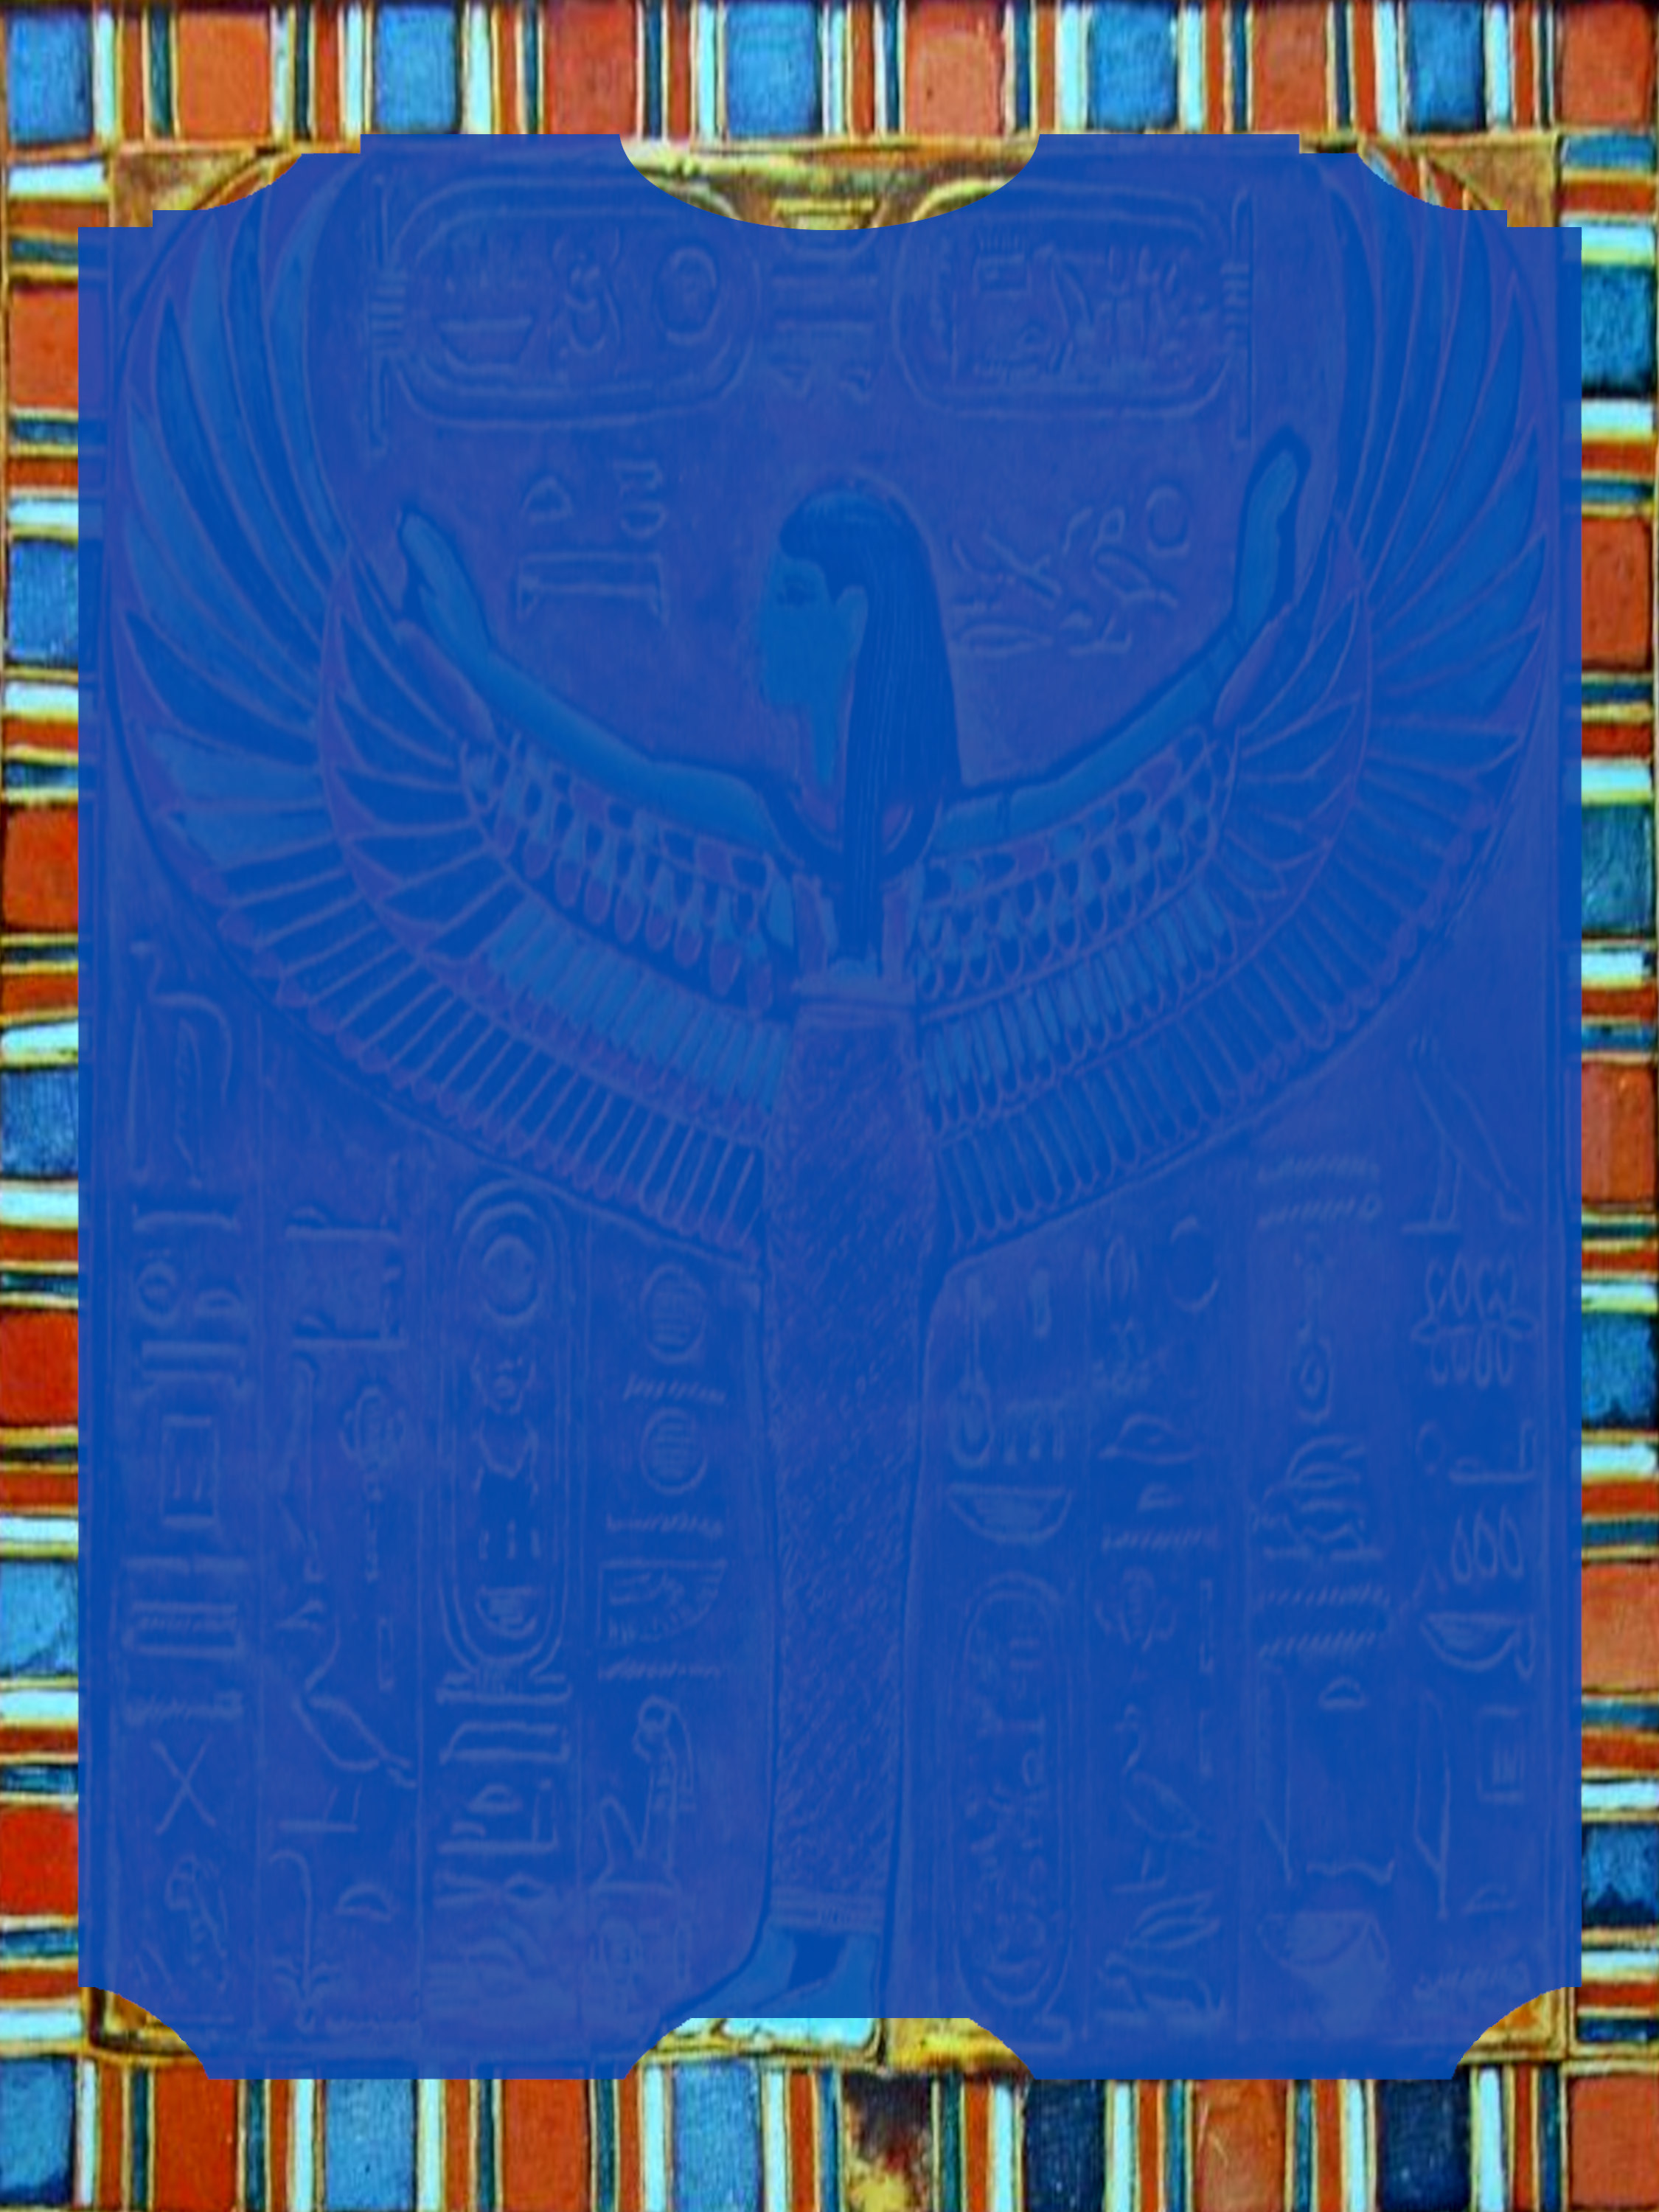
\includegraphics[width=\paperwidth,height=\paperheight]{nut.jpeg}}

\renewcommand{\cftfigfont}{\bfseries}
\renewcommand{\cftfigpagefont}{\bfseries}

\renewcommand{\cftsecfont}{\bfseries}
\renewcommand{\cftsubsecfont}{\bfseries}
\renewcommand{\cftsubsubsecfont}{\bfseries}
% fix toc page numbers
\let\origcftsecfont\cft
\let\origcftsecpagefont\cftsecpagefont
\let\origcftsecafterpnum\cftsecafterpnum
\renewcommand{\cftsecpagefont}{\bfseries{\origcftsecpagefont}}
\renewcommand{\cftsecafterpnum}{\bfseries{\origcftsecafterpnum}}
\let\origcftsubsecpagefont\cftsubsecpagefont
\let\origcftsubsecafterpnum\cftsubsecafterpnum
\renewcommand{\cftsubsecpagefont}{\bfseries{\origcftsubsecpagefont}}
\renewcommand{\cftsubsecafterpnum}{\bfseries{\origcftsubsecafterpnum}}
\let\origcftsubsubsecpagefont\cftsubsubsecpagefont
\let\origcftsubsubsecafterpnum\cftsubsubsecafterpnum
\renewcommand{\cftsubsubsecpagefont}{\bfseries{\origcftsubsubsecpagefont}}
\renewcommand{\cftsubsubsecafterpnum}{\bfseries{\origcftsubsubsecafterpnum}}

\renewcommand{\thefigure}{\bfseries{\arabic{figure}}}

\renewcommand\thefootnote{{\bfseries\color{myRed}\footnotesize{\arabic{footnote}}}}
\let\oldfootnote\footnote
    \renewcommand{\footnote}[1]{\oldfootnote{{\small\bfseries\color{myRed}#1}}}
\bfseries
\begin{titlepage} % Suppresses headers and footers on the title page
	\centering % Centre everything on the title page
	%\scshape % Use small caps for all text on the title page

	%------------------------------------------------
	%	Title
	%------------------------------------------------
	
	\rule{\textwidth}{1.6pt}\vspace*{-\baselineskip}\vspace*{2pt} % Thick horizontal rule
	\rule{\textwidth}{0.4pt} % Thin horizontal rule
	
	\vspace{1\baselineskip} % Whitespace above the title
	
	{\scshape\Huge Le Culte de Neit à Saïs}
	
	\vspace{1\baselineskip} % Whitespace above the title

	\rule{\textwidth}{0.4pt}\vspace*{-\baselineskip}\vspace{3.2pt} % Thin horizontal rule
	\rule{\textwidth}{1.6pt} % Thick horizontal rule
	
	\vspace{1\baselineskip} % Whitespace after the title block
	
	%------------------------------------------------
	%	Subtitle
	%------------------------------------------------
	
	{\scshape \Large Par Dominique Mallet} % Subtitle or further description
	
	\vspace*{1\baselineskip} % Whitespace under the subtitle
	
        {\scshape\scriptsize Ernest Leroux, Editeur} % Subtitle or further description
    
	%------------------------------------------------
	%	Editor(s)
	%------------------------------------------------
        \vspace*{\fill}

	\vspace{1\baselineskip}

	{\small\scshape Paris 1888}
	
	{\small\scshape{Libraire de l'École du Louvre de la Société Asiatique,\\ de l'École des Langues Orientales Vivantes, \emph{etc.} \\ 28 Rue Bonaparte}}
	
	\vspace{0.5\baselineskip} % Whitespace after the title block

        \scshape Internet Archive Online Edition  % Publication year
	
	{\scshape\small Utilisation non commerciale --- Partage dans les mêmes conditions 4.0 International} % Publisher
\end{titlepage}
\setlength{\parskip}{1mm plus1mm minus1mm}
\clearpage
\tableofcontents
\clearpage
\large
\vspace*{\fill}
A M. P. Pierret,

Conservateur du Musée Égyptien,

Professeur à l'École du Louvre.

Hommage Respectueux

D. M.
\vspace*{\fill}
\clearpage
\section*{Préface}
\paragraph{}
\emph{Cet ouvrage est terminé depuis deux ans. Diverses circonstances en ont retardé la publication, et nous le regrettons vivement : car, en Égyptologie comme dans toute science encore jeune, les livres vieillissent très vite.}

\emph{Sur plusieurs des points traités, nos idées se sont assez gravement modifiées et, si nous avions à reprendre la même thèse, nous devrions en ordonner la composition autrement. Mais il ne s'agit pas de la refaire dans cette préface. Il nous convient seulement d'en expliquer l'origine et d'en indiquer la pensée dominante.}

\emph{Des théories nombreuses ont été émises sur l'ensemble de la religion égyptienne. Elles paraissent souvent contradictoires, parce que chacune d'elles s'applique en réalité à une époque différente, et a peut-être le tort d'être trop généralisée. Pour résoudre ces antinomies, il faudrait d'une part étudier les croyances de l'Égypte aux divers moments de son histoire, de l'autre en suivre le développement local dans les milieux où elles sont nées, où elles ont le plus longtemps vécu.}

\emph{La monographie de chaque divinité, ainsi entendue, serait une préparation analytique nécessaire à l'exposé d'une synthèse, qui embrasserait la religion tout entière.}

\emph{On trouvera peut-être que nous avons accordé trop d'importance à l'explication étymologique du nom de notre déesse. La théorie , si brillamment soutenue par M. Max Müller, sur le rôle prépondérant des mots dans la création des personnages mythologiques, paraît aujourd'hui fortement ébranlée. Le fameux} Nomina numina, \emph{qui passait jadis pour une sorte d'axiome, est abandonné maintenant et singulièrement démodé. Nous le savons et ne prétendons point remonter le courant, ni braver l'opinion nouvelle.}

\emph{En Égypte cependant, les noms divins, qui tous sont significatifs, demandent à être examinés de très-près. M. Brugsch l'a montré dans son livre} : Religion und Mythologie der alten Ægypter : \emph{il a même essayé un certain nombre d'étymologies ; il n'a pas rencontré la nôtre, qui pourtant semble se présenter d'elle-même.}

\emph{En fait, nous en avons proposé deux ; mais celle qui, chronologiquement, doit être placée la première} (net = \emph{navette, tissage), avait déjà été indiquée par plusieurs savants. L'autre, celle qui implique un sens métaphysique, nous appartient seule ; et nous croyons qu'elle est incontestable, à condition qu'on ne revendique pas pour elle la priorité, qui revient certainement à l'explication matérielle.}

\emph{A quelle époque faut-il la faire remonter ? La question est évidemment insoluble. Mais il n'y a rien de téméraire à affirmer que la doctrine, qu'elle semble condenser en un mot, existait au moins à l'époque classique, qui commence avec le Nouvel Empire. Elle s'est développée et affinée, compliquée plus tard de mysticisme et de spéculations ingénieuses et profondes. Il est difficile toutefois d'admettre qu'elle ne soit pas plus ancienne.}

\emph{La donnée première, c'est-à-dire l'intelligence du mot} nt \emph{(qui est, où : tu es) doit avoir été acquise de bonne heure. Les conséquences philosophiques ont été tirées plus tard, et chaque siècle a pu les modifier, les compléter à sa guise.}

\emph{Cette explication a le tort de supposer l'existence d'un enseignement ésotérique, qui est aujourd'hui très vivement combattue. Il semble impossible cependant qu'à Saïs au moins
une doctrine secrète n'ait pas été professée parmi les familiers du grand temple et réservée pour certains adeptes, au nombre desquels il faut compter les rois. Nous ne faisons qu'indiquer la difficulté d'ailleurs, et nous n'entendons nullement la trancher.}

\emph{Aucune divinité n'a un caractère local mieux marqué que Neit, bien que son culte se retrouve un peu partout en Égypte. Elle est la maîtresse, la dame de Saïs et du nome Saïte, si bien que les deux noms vont rarement l'un sans l'autre. Aussi est-ce à Saïs qu'on devait retrouver les traits qui caractérisent sa personnalité et les détails qui donnent de son culte l'idée la plus vraie et la plus complète.}

\emph{Voilà pourquoi nous avons jugé utile d'esquisser d'abord à grands traits l'histoire de cette ville, aussi ancienne que la monarchie fondée par Menés, et qui joua un rôle si brillant dans les derniers siècles de l'indépendance.}

\emph{Voilà pourquoi également nous avons donné à ce travail un titre, qui en précise et en détermine exactement les limites. Si étroitement défini dans l'espace, il embrasse au contraire dans le temps toute la durée de la religion égyptienne, et nous avons tâché de suivre les transformations que subit le culte de Neit depuis les premières dynasties Memphites jusqu'aux Ptolémées, c'est-à-dire à l'époque où la pensée grecque, pénétrant peu à peu les vieux dogmes, les modifie en les éclairant par ses interprétations subtiles et ses ingénieux commentaires.}

\emph{Le nom de notre déesse était} Nit, \emph{comme les transcriptions grecques le prouvent surabondamment. Mais il est très connu sous la forme Neit, adoptée dans la plupart des ouvrages qui traitent de mythologie ancienne, et nous avons craint de dérouter le lecteur, en lui imposant une prononciation nouvelle, qui paraît scientifiquement démontrée.}

D. M.
\clearpage
\section{Première Partie. --- Saïs.}
\subsection{Origines. --- Histoire.}
\paragraph{}
Avant d'étudier la cuite de Neit, pour tâcher d'en déterminer avec quelque exactitude le sens et la portée philosophique, il est utile, nécessaire même de connaître la ville, qui lui fut de tout temps consacrée et qui paraît avoir été, en Égypte, le centre principal de son culte.

Cette ville, c'est Saïs.

« Les Égyptiens, dit Brugsch,\footnote{Histoire d'Égypte, éd. de 1875, p. 31.} comme en général les anciens, commençaient la fondation de leurs villes par la construction d'un temple qui formait le centre de la ville à fonder. De nouveaux temples érigés après donnaient l'occasion de créer de nouveaux quartiers qui s'étendaient autour du centre avec lequel ils formaient une seule cité. » Si l'on admet cette manière de voir, le temple de Neit aurait été l'origine de Saïs, comme celui de Ptah dut l'être pour Memphis, celui d'Amon pour Thèbes, \emph{etc.} Ce qui est certain, c'est qu'un hiéroglyphe qui parfois sert à figurer le nom de la déesse avait été adopté comme la dénomination ordinaire du nome dont Saïs était le chef-lieu $\hieroAAAA$, et fut souvent employé pour désigner ce chef-lieu lui-même $\hieroAAAB\:\hieroAAAC$. Les variantes sont nombreuses d'ailleurs et voici les principales qui ont été relevées sur les monuments\footnote{V. \emph{Brugsch.} Dictionn. géogr., p. 245.} : $\hieroAAAD\:\hieroAAAC$, $\hieroAAAE$, $\hieroAAAD\:\hieroAAAF$, $\hieroAAAD\:\hieroAAAG\:\hieroAAAH\:\hieroAAAH\:\hieroAAAC$,\footnote{On trouve encore $\hieroAAAV\:\hieroAAAW$ dans \emph{Sharpe} Inscript. 1, 16. Mais ce nom s'applique-t-il véritablement à Saïs ? --- Sais est désignée aussi par le groupe $\hieroAAAS\:\hieroAAAC$, $\hieroAAAT\:\hieroAAAH\:\hieroAAAH\:\hieroAAAU$ qui est traduit en Grec par ἀνδρῶνπόλις.} démotique : $\demotiqueone$, copte : \begin{coptic}cai\end{coptic} ; (arabe : \novocalize{\RL{.sA}} ; assyrien : $\assyrianniaa$ ; hébreu : \foreignlanguage{hebrew}{\<MAy>}.)

Quelle est l'étymologie du mot ? On ne peut émettre là-dessus que de simples conjectures. Le mot $\hieroAAAI\:\hieroAAAK$, $\hieroAAAI\:\hieroAAAL$ qui signifie sol se présente le premier à la pensée. D'autre part, on trouve, dans les hiéroglyphes, le groupe $\hieroAAAM\:\hieroAAAN$ avec le sens de tissu. Or comme nous le ferons remarquer plus loin, le déterminatif le plus habituel du nom de Neit, $\hieroAAAO$, semble se rapporter à l'idée du tissage. On pourrait encore rapprocher du nom de Saïs le mot $\hieroAAAP$ qui signifie lancer des flèches, et qui se réfère à une autre forme du déterminatif ajouté au nom de Neit dès les temps de l'Ancien Empire : $\hieroAAAQ\:\hieroAAAR$.\footnote{On a prétendu que Saïs signifiait olivier, à cause de l'hébreu \foreignlanguage{hebrew}{\<zayit>} Mais Wilkinson, (Manners and Customs, 3, 40) observe avec raison que le nome Saïte n'était pas renommé pour la culture de l'olivier. C'est l'assimilation de Neit à Minerve qui a été cause de cette erreur. Diod. (liv. 1, 16) dit que les Égyptiens attribuaient le don de l'olivier à Hermès.} Ces diverses observations nous amènent à reconnaître, que très probablement le nom de la ville lui est venu de la déesse qui y fut principalement honorée.

Elle était située à quelque distance de la branche occidentale du Nil (Canopique), à 60 kilomètres environ dans l'intérieur des terres, près de l'emplacement occupé aujourd’hui par un village du nom de \emph{Ssa el Hagar}, à 110 kilomètres, à vol d'oiseau, de l'ancienne Memphis.\footnote{d'Anville, ce géographe qui fit plus d'une découverte sans sortir de son cabinet, avait déterminé, d'une manière exacte, la position de Sais. --- \emph{Ssa el Hagar} est à 2 kilomètres du Nil, sur la rive droite ; les ruines de Saïs sont au N. de ce village.}

Le nome Saïte, dont elle était la capitale, se divisait en deux parties : $\hieroAAAB\:\hieroAAAX$, du Midi et : $\hieroAAAB\:\hieroAAAY$, du Nord. Sais était dans la partie septentrionale du nome.\footnote{\emph{Lepsius}, Denkm. 4, 79, e : $\hieroAAAZ\:\hieroAABA\:\hieroAABB\:\hieroAABC\:\hieroAABD\:\hieroAABE$.}

Il paraît probable aujourd'hui, contrairement à l'opinion des anciens, que la civilisation en Égypte a remonté le Nil, au lieu de le descendre. Bien que la première race royale soit, dit-on, originaire de Thinis, elle semble avoir établi à Memphis le principal centre de sa domination politique et le plus solide boulevard du pays contre les invasions des peuples de l'orient et de l'occident, de la Syrie et de la Libye. Plusieurs des villes du Delta existaient déjà sans doute lorsque Mena, ayant détourné le Nil, se décida à fonder Memphis.

Saïs du moins fut certainement contemporaine des plus anciennes dynasties. Dans les tombeaux de Saqqarah et de Gizeh, des 4\textsuperscript{e}, 5\textsuperscript{e} et 6\textsuperscript{e} dynasties, si nous ne voyons pas paraître le nom même de Saïs, nous rencontrons fréquemment celui de sa divinité éponyme, \emph{Neit}. Peut-être même, lorsque le nom de \emph{Neit} ($\hieroAAAQ$) est accompagné du signe $\hieroAABF$, ce dernier a-t-il précisément le sens que prend plus tard le hiéroglyphe plus complet $\hieroAAAA$, et l'ensemble signifie-t-il : \emph{Neit} de Saïs ou du nome Saïte. Ce n'est là qu'une hypothèse.

Mais nous avons mieux que des hypothèses pour prouver l'ancienneté de Saïs ; nous possédons des textes gravés ou écrits, dont l'autorité est irrécusable.

Dans le tombeau d'\emph{Amten} un des plus anciens monuments connus, puisqu'il s'agit d'un fonctionnaire de \emph{Snefru} (3\textsuperscript{e} dynastie),\footnote{Aujourd'hui au Musée de Berlin 5. \emph{Lepsius}, Denkm. part. 2, pl. 3-7.} au milieu des titres du défunt, qui fut gouverneur de plusieurs villes et localités de la Basse-Égypte, on trouve des indications précieuses. L'interprétation de ces titres, vu l'extrême ancienneté du monument, offre des difficultés très-grandes.

Il en est un qui revient plusieurs fois dans les cinq planches des \emph{Denkmaeler} consacrées au tombeau d'Amten. Il est écrit $\hieroAABG\:\hieroAABH$ dans le premier exemple (pl. 3), et ici la difficulté est double. Car nous ne savons encore ni la prononciation, ni le sens exact du premier groupe. Chabas le livait \emph{χamer} confondant le signe $\hieroAABI$ avec celui de $\hieroAABJ$, qui paraît en différer sensiblement et qui, en effet, se lit ordinairement \emph{χa}.

Plus loin, à la même planche, se trouvent les titres suivants : $\hieroAABK\:\hieroAABL\:\hieroAABM\:\hieroAABN\:\hieroAABO\:\hieroAABP$ docteur, chef des sacrifices, chef de la grande demeure, ....

Au milieu, dans les lignes horizontales, à la fin de la série des titres, nous rencontrons de nouveau le $\hieroAABG\:\hieroAABP$ place en dernier lieu avant le nom d'$\hieroAABQ\:\hieroAABR\:\hieroAABS$. Jusque-là le dessin manque de netteté, mais, sur le petit montant de gauche, il reparaît beaucoup plus clair, et de manière à ne plus laisser de doute : $\hieroAABG\:\hieroAABT$. Ici, il s'agit bien évidemment des deux flèches croisées. Le même idéogramme figure de nouveau aux planches 5, 6 et 7, et cette fois encore il est dessiné avec une perfection, qui ne laisse place à aucune ambiguïté.

M. Pierret, qui a traduit complètement les inscriptions de cette dernière planche, interprète ainsi : « Son père l'a fait inscrire comme gouverneur des gens de Tep, chef du palais du domaine $\hieroAABU\:\hieroAABV$, du domaine Sepa, gouverneur du nome de Neit $\hieroAABG\:\hieroAABW$. » Ce nome de Neit (\emph{Neit hesep}) est bien évidemment le nome Saïte. La ville elle-même n'est pas nommée, mais nous avons du moins la mention du district dont elle était le chef-lieu, et nous pouvons conclure de l'existence du nome à l'existence de la cité, qui renferma dès l'origine le temple où Neit était spécialement adorée.

La pyramide d'Ounas (dernier roi de la 5\textsuperscript{e} dynastie), dont les textes ont été publiés et traduits par M. Maspero, est plus explicite. Elle nous présente le nom de Saïs écrit phonétiquement, et de la manière la plus complète. On trouve en effet, à la ligne 556, une invocation ainsi conçue : $\hieroAABX\:\hieroAABY\:\hieroAABZ\:\hieroAAAI\allowbreak\:\hieroAACA\:\hieroAACB\:\hieroAAAW\:\hieroAABR\:\hieroAACC\allowbreak\:\hieroAACD\:\hieroAAAH\:\hieroAACE\:\hieroAAAH\allowbreak\:\hieroAAAH\:\hieroAACF\:\hieroAACB\:\hieroAACG\allowbreak\:\hieroAACH\:\hieroAACI\:\hieroAAAH\:\hieroAACJ\allowbreak\:\hieroAACK\:\hieroAACL\:\hieroAACM\:\hieroAACN\:\hieroAACO\allowbreak\:\hieroAACO\:\hieroAACP\:\hieroAACQ\:\hieroAACN\allowbreak\:\hieroAAAH\:\hieroAACR\:\hieroAACS\:\hieroAACT\:\hieroAACU$ ô siège de Saïs, grâce à la traversée ... que fait \emph{χnum} apportant ces choses à \emph{Unas}, c'est \emph{Unas Sokari} au \emph{Rosta-u}, \emph{etc.}

Dans le \emph{Todtenbuch}, qui est composé de plusieurs parties d'époques différentes, mais dont le fond remonte à une très haute antiquité, puisqu'on en retrouve la plupart des chapitres dans les plus anciens tombeaux, Saïs apparaît à plusieurs reprises.

Ainsi, au Ch. 42, 1. 6, où Neit est appelée dame de Saïs, $\hieroAACV\:\hieroAABC\:\hieroAACW\:\hieroAACX\:\hieroAACY$. Au Ch. 142, où, dans la Litanie d'Osiris, il est dit, A l. 23 : Osiris dans Saïs, $\hieroAACZ\:\hieroAADA\:\hieroAAAI\allowbreak\:\hieroAAAG\:\hieroAAAF\:\hieroAADB$ ; puis, B, l. 3 et 4 : $\hieroAACZ\:\hieroAADA\:\hieroAAAI\allowbreak\:\hieroAADC\:\hieroAAAW\:\hieroAADD\:\hieroAADB$ et : $\hieroAACZ\:\hieroAABR\:\hieroAAAD\:\hieroAADC\:\hieroAAAW\:\hieroAADE\:\hieroAADB$ Osiris dans Saïs inférieure, et : Osiris dans Saïs supérieure.

Une phrase célèbre et souvent citée du Ch. 163, l. 13,\footnote{Ce chap. et ceux qui le suivent paraissent plus récents que les précédents, comme l'indiquent les quelques lignes que le scribe y a mises en guise de préface. Nous ne le citons donc ici que pour mémoire.} dit : « L'Osiris N. est avec l'esprit parfait, il est l'âme du grand corps qui est à Saïs, \emph{Neit} : $\hieroAAAH\:\hieroAADF\:\hieroAACR\:\hieroAADG\allowbreak\:\hieroAADH\:\hieroAADI\:\hieroAADB\:\hieroAAAH\allowbreak\:\hieroAADJ\:\hieroAADK\:\hieroAADL\:\hieroAADM\allowbreak\:\hieroAADN\:\hieroAACN\:\hieroAADO\allowbreak\:\hieroAADP\:\hieroAADQ\:\hieroAADR\:\hieroAABR\allowbreak\:\hieroAAAD\:\hieroAAAG\:\hieroAADC\:\hieroAAAW\allowbreak\:\hieroAAAQ\:\hieroAACY$.

Enfin, le Ch. 125, la confession négative, nous apprend que trois des juges des Enfers avaient été choisis à Saïs. On lit en effet, l. 21 : « ô porteur d'aliments, sorti de Saïs, je n'ai pas été bravache. » $\hieroAAAH\:\hieroAADF\:\hieroAACJ\:\hieroAACN\allowbreak\:\hieroAADS\:\hieroAADT\:\hieroAADU\:\hieroAADV\allowbreak\:\hieroAAAD\:\hieroAAAG\:\hieroAADC\:\hieroAAAW\allowbreak\:\hieroAADB\:\hieroAADW\:\hieroAADU\allowbreak\:\hieroAADX\:\hieroAADF$ ; --- L. 25 : « ô maître de la double corne, sorti de Saïs, je n'ai pas multiplié les paroles en parlant, » $\hieroAAAH\:\hieroAADF\:\hieroAABC\allowbreak\:\hieroAADY\:\hieroAADY\:\hieroAADU\allowbreak\:\hieroAADV\:\hieroAAAD\:\hieroAAAG\allowbreak\:\hieroAADC\:\hieroAAAW\:\hieroAADB\allowbreak\:\hieroAADW\:\hieroAADZ\:\hieroAAEA\allowbreak\:\hieroAACM\:\hieroAADF\:\hieroAAEB\allowbreak\:\hieroAAEC\:\hieroAAED\:\hieroAAEE\allowbreak\:\hieroAADF\:\hieroAAEF$ et l. 30 : « ô celui qui fait prospérer les intelligents, sorti de Saïs, je n'ai pas conjuré Dieu, $\hieroAAAH\:\hieroAADF\:\hieroAAEG\allowbreak\:\hieroAAEH\:\hieroAAEI\:\hieroAADU\allowbreak\:\hieroAADV\:\hieroAAAD\:\hieroAAAG\allowbreak\:\hieroAADC\:\hieroAAAW\:\hieroAADB\allowbreak\:\hieroAADW\:\hieroAAEJ\:\hieroAADF\allowbreak\:\hieroAAEB\:\hieroAAEK\:\hieroAADB$.

Un livre, dont nous ne possédons qu'une copie relativement récente, mais dont la rédaction primitive devait remonter fort loin, nous offre aussi plusieurs mentions de Saïs, cette fois à propos d'Osiris, considéré comme fils de Neit, et il est ainsi parfaitement d'accord avec les passages du Ch. 42 que nous venons de reproduire. C'est le livre des \emph{Lamentations d'Isis et de Nephthys}.\footnote{\emph{De Horrack} : Les Lamentations d'Isis et de Nephthys.} \emph{Nephthys} dit, dans une de ses invocations, p. 5, l. 5 et suiv. : « ô Dieu An, viens à Saïs ! Saïs est ton nom. Viens à Aper, tu verras ta mère Neit. Bel enfant, ne t'arrête pas loin d'elle. Viens à ses mamelles, t'y abreuver. Frère excellent, ne t'arrête pas loin d'elle ! ô fils, viens à Saïs ! » $\hieroAAEL\:\hieroAAEM\:\hieroAADG\allowbreak\:\hieroAAEN\:\hieroAAEO\:\hieroAAEP\allowbreak\:\hieroAAAD\:\hieroAAEQ\:\hieroAADC\allowbreak\:\hieroAAAW\:\hieroAAAD\:\hieroAAAG\allowbreak\:\hieroAADC\:\hieroAAAW\:\hieroAAFU\allowbreak\:\hieroAACM\:\hieroAAER\:\hieroAADB\allowbreak\:\hieroAAES\:\hieroAADG\:\hieroAAEN\allowbreak\:\hieroAAET\:\hieroAAEU\:\hieroAAAW\allowbreak\:\hieroAAEV\:\hieroAAEW\:\hieroAACY\allowbreak\:\hieroAAES\:\hieroAAEX\:\hieroAAEY\allowbreak\:\hieroAAEZ\:\hieroAAFA\:\hieroAAFB\allowbreak\:\hieroAAEM\:\hieroAADW\:\hieroAAFC\allowbreak\:\hieroAAFD\:\hieroAAFE\:\hieroAAFF\allowbreak\:\hieroAADG\:\hieroAAAH\:\hieroAAFG\allowbreak\:\hieroAAFH\:\hieroAAFI\:\hieroAAFJ\allowbreak\:\hieroAAFD\:\hieroAAFK\:\hieroAAEZ\allowbreak\:\hieroAACM\:\hieroAAFL\:\hieroAAFM\allowbreak\:\hieroAAAH\:\hieroAABR\:\hieroAAFN\allowbreak\:\hieroAAFO\:\hieroAAAH\:\hieroAADB\allowbreak\:\hieroAAFB\:\hieroAAEM\:\hieroAADW\allowbreak\:\hieroAAFC\:\hieroAAFD\:\hieroAAFE\allowbreak\:\hieroAAFF\:\hieroAAAH\:\hieroAADF\allowbreak\:\hieroAAAI\:\hieroAADB\:\hieroAADG\allowbreak\:\hieroAAAH\:\hieroAAEO\allowbreak\:\hieroAAEP\:\hieroAAAD\allowbreak\:\hieroAAEQ\:\hieroAADC\:\hieroAAFP$. Et plus loin, l. 8 : « ô excellent souverain ! Viens à ta demeure ; seigneur de Saïs, viens à Saïs ! $\hieroAAAH\:\hieroAADF\:\hieroAAAH\allowbreak\:\hieroAACD\:\hieroAAAH\:\hieroAAAH\allowbreak\:\hieroAAFQ\:\hieroAADB\:\hieroAAFB\allowbreak\:\hieroAAFV\:\hieroAADG\:\hieroAAAH\:\hieroAAEO\allowbreak\:\hieroAAEP\:\hieroAAFR\:\hieroAAFS\:\hieroAAAD\allowbreak\:\hieroAAEQ\:\hieroAADC\:\hieroAAFT\:\hieroAADG\allowbreak\:\hieroAAAH\:\hieroAAEO\:\hieroAAEP\allowbreak\:\hieroAAAD\:\hieroAAAG\:\hieroAADC\:\hieroAAFT$.

Des textes que nous venons de réunir, les uns sont expressément datés, les autres se rattachent très vraisemblablement aux origines mêmes de la religion égyptienne. Leur ensemble concourt donc à prouver jusqu'à l'évidence que Saïs existait aux premiers temps de l'Égypte et que, dès lors, elle était le sanctuaire préféré, la résidence même d'une des déesses les plus vénérées du pays, de Neit.

Osiris y figurait à côté d'elle, et comme son fils. Or, nous verrons que ces deux divinités sont de celles qui, de très-bonne heure, reçurent des hommages dans toute l'étendue de la contrée. La renommée de la ville sainte, qu'elles avaient choisie, pour leur demeure de prédilection, se répandait donc aussi loin que leur culte. Partout où il était question de Neit et de sa puissance, il était en même temps question de Saïs.

Maintenant, quelle place a tenue Saïs dans l'ensemble de la civilisation égyptienne ? En nous adressant aux textes d'une part, et de l'autre aux récits des historiens grecs, nous prouverons qu'elle a joué, à des époques diverses, un rôle considérable dans l'industrie, dans la religion, dans la politique et dans l'art.

C'est à Neit, la patronne de Saïs, qu'on attribuait l'invention de l'art de tisser, et, comme nous l'avons dit, l'idéogramme de son nom semble une allusion permanente à ce souvenir légendaire. D'après le témoignage des monuments, sa ville se distinguait en effet dans la fabrication des étoffes et des tissus. Un des sanctuaires de Saïs, le \emph{Ha-χeb} $\hieroAAFW$ est aussi appelé $\hieroAAFX$, la maison des étoffes.\footnote{V. Dendérah, texte des mystères d'Osiris, col. 22. Cf. \emph{Mariette}, Abydos, pl. 63.} Les $\hieroAAFY\:\hieroAAFZ\:\hieroAAGA\allowbreak\:\hieroAADV\:\hieroAAAX\:\hieroAADR\allowbreak\:\hieroAAAU\:\hieroAAGB\:\hieroAAAU$, les quatre étoffes dans la demeure du S. et dans la demeure du N. (localités du district de Saïs), ont une grande importance dans la pratique du culte.\footnote{Dans le temple de Minerve à Athènes (la déesse assimilée à Neit par les Grecs), on travaillait aussi sous la surveillance de la prêtresse. Pendant neuf mois, des jeunes filles et des femmes, habiles dans l'art de la tapisserie, ἐργατῖναι, fabriquaient le peplos, qu'on offrait chaque année à Athènè et qu'on portait dans l'Érechthéion. Au jour de la fête, le peplos déployé était tendu comme une bannière, ou plutôt comme une voile de vaisseau, au-dessus de la trirème sacrée, emblème de la puissance maritime qu'Athènes devait à la déesse, et qui, mise en mouvement par de puissantes machines, gravissait les pentes de l'Acropole, avec le cortège sacré. (\emph{Decharme}, Mythol. de la Grèce antique, 91. --- Cf. \emph{L. de Ronchaud}, le Péplos d'Athènè, Rev. archéol.)}

Dans le papyrus de Téos, au Louvre, on lit : $\hieroAACS\:\hieroAAGC\:\hieroAAAG\allowbreak\:\hieroAABR\:\hieroAAFZ\:\hieroAACS\allowbreak\:\hieroAAGD\:\hieroAABR\:\hieroAAAX\allowbreak\:\hieroAAAQ\:\hieroAAAC\:\hieroAAGE\allowbreak\:\hieroAAAW\:\hieroAAGF\:\hieroAAGG\allowbreak\:\hieroAABR\:\hieroAAGH\:\hieroAACN\:\hieroAACS\allowbreak\:\hieroAAFD\:\hieroAAGI\:\hieroAAEK\allowbreak\:\hieroAAEK\:\hieroAAEF$ elle (\emph{Neit}) t'habille dans la demeure du S. et dans la demeure du N. d'étoffes faites par les dieux \emph{Sebek},\footnote{L'hymne de \emph{Hib} à \emph{Amon} dit également : $\hieroAAGJ\:\hieroAAGK\:\hieroAACM\allowbreak\:\hieroAAEZ\:\hieroAAGL\:\hieroAAGM\allowbreak\:\hieroAAAX\:\hieroAAGN\:\hieroAAGO\:\hieroAAGP\allowbreak\:\hieroAAGQ\:\hieroAAGR\allowbreak\:\hieroAAGS\:\hieroAAGT$ l'étoffe rouge couvre ton corps dans les demeures du S. et du N. Tes tissus sont placés sur les mains des deux \emph{Sebek} (col. 28). --- Tous ces textes sont empruntés au Dict. géogr. de Brugsch, p. 1174.} Ces citations montrent que certaines parties du temple de \emph{Neit} étaient spécialement consacrées à la confection de tissus d'une espèce particulière, dont on faisait usage dans les cérémonies sacrées, et qui servaient sans doute à l'habillement des prêtres et aussi à l'habillement des statues et des momies.\footnote{Les prêtres de Neit sont dits : linigeri. De plus, Cf. \emph{Eustath} in Iliad. A, 31 : πρώτη δέ τις Αἰγυπτία γυνὴ καθεζομένη ὕφανεν ἀφ᾽ἧς καὶ Αἰγύπτιοι Ἀθηνᾶς ἄγαλμα καθημένης ἱδρύσαντο.}

Ainsi, dans le Rituel de l'embaumement traduit par M. Maspero, on voit que les mains et les pieds de la momie étaient enveloppés « d'une tresse de lin, de celles qu'on fabrique à Saïs.\footnote{Pap. 3 de Boulaq, 3, 15. \emph{Maspero}, Mém. sur sqq. Papyrus du Louvre, p. 22.} » Dans le même document, il est dit encore : « On t'a fait une tresse de Saïs pour amulette préservateur ; Neit veille sur toi dans Tesut.\footnote{Pap. 3 de Boulaq, 4, 6 ; \emph{Maspero}, p. 24.} »

Il y avait là évidemment de véritables ateliers-modèles, ayant un caractère religieux. Bien que les procédés qu'on y employait fussent peut-être tenus secrets, les artisans de la cité de \emph{Neit} s'honoraient de travailler, eux aussi, à des ouvrages analogues, quoique d'une qualité moindre.

Ainsi la ville et son nome durent jouir, à une époque très reculée, d'une remarquable prospérité industrielle. De plus, aucune contrée n'était plus heureusement placée pour les échanges, et les premières relations commerciales qui s'établirent avec l'extérieur profitèrent certainement à Saïs et à ses plus proches voisines.

Hérodote, qui a été trompé si étrangement par ses interprètes égyptiens sur la succession des dynasties, s'accorde néanmoins avec les monuments pour montrer que Saïs fut de très bonne heure une ville sacrée. Les histoires qu'il rapporte au sujet de Mycérinus $\hieroAAGU$ sont le reflet de légendes assurément très anciennes, puisque ce roi est classé justement par Manéthon dans la 4\textsuperscript{e} dynastie. D'après les légendes auxquelles nous faisons allusion, cet excellent souverain, cruellement frappé par les dieux malgré ou plutôt à cause de sa piété, aurait voulu ensevelir sa fille trop chérie en enfermant le cadavre dans une génisse de bois doré. L'écrivain grec assure qu'elle était encore de son temps dans la demeure royale, à Saïs, et il a vu, dans une chambre voisine, les vingt-quatre statues de bois des concubines de Mycérinus. « La génisse dit-il, a le corps couvert d'une housse de pourpre, hormis le cou et la tête, qui sont plaqués d'épaisses lames d'or ; entre ses cornes brille le cercle du soleil, imité en or ; elle ne se tient pas droite, mais sur les genoux ; sa taille est celle d'une grande vache vivante.\footnote{\emph{Herod.}, l. 2, c. 132.} »

A propos des contes que lui ont fait les prêtres sur Mycérinus, Hérodote exprime des doutes, qui ne sont que trop fondés. Mais, quant à la génisse, il l'a vue de ses yeux, ainsi que les statues de bois, qui représentaient des femmes nues. « Qui sont-elles ? ajoute-t-il, je n'en puis dire que ce que l'on m'a raconté. »

Quoiqu'il en soit, de toutes ces légendes plus ou moins embellies, altérées au cours des siècles, il résulte que, dans l'imagination populaire et aussi dans la tradition des temples, le nom de Saïs était, au même titre que celui de Memphis, inséparable du souvenir des premiers souverains de l'Égypte.\footnote{Nous citerons ici une curieuse tradition arabe, rapportée par l'historien Makrisy, et qui fait voir, d'après des données encore purement légendaires, l'opinion qu'on a eue de tout temps de l'ancienneté de Saïs. Mizraïm, qui, après le déluge, avait choisi pour sa demeure et pour celle de ses descendants, tout le pays qui s'étend depuis l'Égypte jusqu'à l'extrémité de l'Afrique, laissa quatre enfants : \emph{Ischemun, Atrib, Sa} et \emph{Copt.} Il leur divisa l'Égypte en quatre parties égales. \emph{Copt} eut toute cette étendue, qui est depuis Isvan jusqu'à la ville de Copt. Il donna à Ischemun tout ce qui est depuis la ville de Copt jusqu'à Menuf. Atrib eut en partage le ventre de l'Égypte, qui est ce que nous appelons le Delta. Et Sa eut tout ce qui va depuis la province de Beheire jusqu'à la Barbarie inclusivement. Chacun d'eux fit bâtir une ville dans ses états, à laquelle il donna son nom. (V. \emph{Vansleb}, Nouv. relation d'un voyage en Égypte. Paris, 1677).}

La position géographique qu'elle occupait, a si peu de distance de la mer, dans le voisinage de la Libye, et non loin de l'isthme de Suez, la prédestinait à recevoir les influences du dehors.

Lorsque la terrible invasion des Pasteurs se répandit comme un torrent, le Delta, occupe le premier et entièrement possédé par les Sémites jusqu'au jour de leur définitive expulsion, ressentit, plus que les autres parties du pays, les effets de la conquête.

Les tribus de même race, qui, comme celle des Hébreux, vinrent, à leur suite et avec leur agrément, s'établir dans certains cantons du Nord, s'y multiplièrent rapidement. Elles apportaient des ferments nouveaux, propres à modifier sensiblement les coutumes, les idées de leur patrie d'adoption : et même après leur départ, le séjour prolongé qu'elles y avaient fait ne pouvait manquer de laisser des traces profondes.

Ce que les croisades ont fait, au moyen-âge pour les peuples occidentaux, les expéditions militaires des Thoutmès et des Ramsès le firent pour l'Égypte 1500 à 1800 ans avant notre ère. La terre des Pharaons, jusqu'alors rebelle à tout ce qui venait de l'extérieur, devint accessible aux nouveautés apportées de l'Orient et du Nord. Elle y perdit pour l'originalité, l'unité des vues, le caractère, tout ce qui fait la forte personnalité d'une nation. Elle s'humanisa, pour ainsi dire ; les habitants de la terre noire $\hieroAAGV\:\hieroAAGW\:\hieroAAAW$ se laissèrent aller à un enthousiasme presque excessif pour les choses de l'Asie. On prit modèle sur ceux qu'on avait longtemps méprisés comme des barbares. On leur emprunta ce qui manquait à l'Égypte ; et la mode s'en mêlant, on affecta d'imiter jusqu'à leur langage. Un commerce ininterrompu s'établit entre des peuples autrefois isolés. Mais ces relations ne furent pas toujours pacifiques. Les Égyptiens avaient appris le chemin de l'Asie ; les Assyriens et les Perses apprendront aussi celui de l'Égypte, et les revanches seront terribles.

Au temps de la colonisation Sidonienne, les Phéniciens, en récompense de leur soumission aux successeurs de Thoutmès 1, avaient obtenu, par une convention tacite, le privilège du commerce de l'Égypte. Ils y fondèrent, non pas des colonies, mais des comptoirs, dont quelques-uns, avec les années, prirent de sérieux développements. Saïs en avait un, aussi bien que Bubaste, Mendès, Tanis et Memphis.\footnote{\emph{Maspero}, hist. anc. des peuples de l'Orient, p. 237.} Avec eux s'implantait dans le Nord cette influence orientale, que les courses des Pharaons de la 17\textsuperscript{e} et de de la 18\textsuperscript{e} dynastie à travers l'Asie antérieure servirent si puissamment, en établissant un contact journalier entre les conquérants et les nations vaincues. Saïs devint dès lors. ainsi que d'autres grandes villes du Delta, un des points principaux où s'opéra le mélange des peuples et la pénétration réciproque des idées.

D'un autre côté, les peuplades guerrières, sédentaires ou nomades, qui couvraient le Nord de l'Afrique, à l'Ouest, et que l'on a coutume de grouper sous la dénomination générale de Libyens, s'avancèrent bientôt jusque dans les parties les plus occidentales du Delta. Soumis par les rois des premières dynasties, avec des alternatives de révoltes sévèrement réprimées, depuis Mena jusqu'à Seti 1, ces barbares firent partie alors de la redoutable coalition des peuples méditerranéens, qui échoua devant l'énergie du jeune Ramsès. Ils revinrent sous Meneptah 1 ; ils revinrent sous Ramsès 3 (20\textsuperscript{e} dynastie). Malgré les défaites sanglantes qui leur furent infligées à plusieurs reprises, ils trouvèrent moyen de se cantonner solidement dans les nomes Maréotique et Saïtique, et jusqu'aux environs de Memphis. Le roi, après les avoir vaincus, au lieu de les chasser du pays, songea à utiliser leurs services, il les incorpora dans son armée, à titre de troupes auxiliaires, il en fit ses gardes du corps.\footnote{Au temps d'Hérodote, Saïs était, comme Busiris, Chemmis, Paprémis, l'île de Prosopitis et la moitié de Natho, une des résidences assignées aux Hermotybies, l'une des classes des guerriers. « Les Hermotybies, ont, dit-il, leurs domaines sur ces nomes ; leur nombre est de cent soixante mille hommes, quand ils sont au grand complet. Nul d'entre eux n'a jamais rien appris des arts mécaniques, mais ils se consacrent au métier des armes. » (\emph{Herod.} 2, 165).}

Ceux-là n'apportaient point avec eux, comme les colons de l'Orient, les avantages et les défauts d'une civilisation avancée et toute différente de celle de l'Égypte. Soldats avant tout, promptement rompus aux habitudes de la discipline militaire, ils subirent, sans même essayer d'y résister, l'action du milieu nouveau, où les avait introduits le hasard d'entreprises manquées. Mais en se fixant dans le pays de leurs nouveaux maîtres, ils vinrent augmenter, d'un élément plus jeune et encore à demi sauvage, la complexité d'une population déjà si étrangement mêlée. Vers la fin de la 20\textsuperscript{e} dynastie, ils étaient devenus les favoris des Pharaons, et bientôt les rudes chefs des Mašuaš allaient être assez forts pour dicter des lois à leurs prétendus souverains.\footnote{\emph{Maspero}, hist. p. 358.}

Avec le progrès des temps, la vie semblait se retirer de Thèbes et des nomes du Sud pour remonter vers l'extrémité opposée. Après avoir lutté bravement contre les coalitions étrangères et arrêté des invasions redoutables, la 20\textsuperscript{e} dynastie s'éteint obscurément au milieu des révolutions de palais. Tandis que des Ramessides, réduits à l'état de rois fainéants, végètent encore sur le trône du Midi, le Nord, travaillé par les influences multiples que nous avons indiquées, revendique à son tour la suprématie.

Il a des princes ambitieux, avides de pouvoir, --- Sémites, Libyens, Égyptiens de sang mêlé, --- qui, sous prétexte de protester contre l'usurpation des grands-prêtres d'Amon, aspirent à remplacer la dynastie dépossédée. Tanis entre la première en scène avec Simentu Meiamoun (Smendès), qui inaugure la 21\textsuperscript{e} dynastie. L'autorité de ses rois n'est solidement affermie que dans le Nord. Les contrées lointaines se révoltent, et, sous les faibles successeurs de Simentu, plusieurs d'entre elles se détachent complètement du vieux tronc égyptien. Les rois eux-mêmes consacrent, par leur exemple, la confusion des races, en acceptant pour leurs propres enfants des alliances avec les princes barbares.

Ces tendances antinationales s'accentuent davantage encore sous les rois bubastites, Libyens d'origine, les Sešonk, les Osorkon et les Takelot ; et les Tanites de la 23\textsuperscript{e} dynastie ne sont ni d'humeur ni de taille à changer la direction du courant.

Les dieux de Syrie, Baal, Astarté, Qadeš, révérés avec quelque effroi au temps des Ramessides, comme des ennemis dont on veut prévenir la colère ou apaiser le ressentiment, deviennent désormais des maîtres reconnus, les égaux des divinités indigènes. On ne leur sacrifie pas seulement par crainte, on les adore, on les aime comme des protecteurs naturels, qui rappellent la patrie et la religion des ancêtres.

Au milieu des princes du Delta qui se disputaient l'hégémonie, les Saïtes se distinguent par la netteté de leurs vues politiques et par l'énergie de leur caractère. Tafneχθ le premier rêve d'abattre les roitelets qui se partagent le pouvoir et de reconstruire, à son profit, l'empire des Pharaons.\footnote{Dans la stèle de Pianχi, l. 19-20, les titres de Tafneχθ sont ceux-ci : $\hieroAAFQ\:\hieroAAGX\:\hieroAAGY\allowbreak\:\hieroAABM\:\hieroAAGZ\:\hieroAAHA\allowbreak\:\hieroAAHB\:\hieroAAEK\:\hieroAAHC\allowbreak\:\hieroAAHJ\:\hieroAABC\allowbreak\:\hieroAAHD\:\hieroAAAC\:\hieroAACS\allowbreak\:\hieroAABR\:\hieroAAEB\:\hieroAACN\:\hieroAAHE\allowbreak\:\hieroAAEZ\:\hieroAAEK\:\hieroAACB\:\hieroAAAG\allowbreak\:\hieroAAHF\:\hieroAACD\:\hieroAAEB$ discours où Tafneχθ demande grâce à Pianχi, il dit (l. 136) : $\hieroAAEP\:\hieroAACS\:\hieroAADS\allowbreak\:\hieroAAHG\:\hieroAAEB\:\hieroAAHJ\allowbreak\:\hieroAACY\:\hieroAAHH\:\hieroAAHI$, je me suis confié à Neit tout à fait en me cachant.} Mais quelques-uns de ses rivaux appellent Pianχi à leur secours, et c'est l'Ethiopien victorieux qui rétablit, pour quelques années, l'unité, tout en laissant à ses vassaux l'autorité sur leurs nomes respectifs. Le fils de Tafneχt, Bok-n-ranf parvient à réaliser les projets de son père, et il constitue, à lui seul, la première dynastie Saïte (24\textsuperscript{e}). Mais l'Ethiopie l'emporte de nouveau avec Šabak, qui renverse le malheureux Bok-n-ranf et lui fait subir, dit-on, le plus cruel des supplices.

Cependant les Assyriens s'avancent à grands pas vers l'Afrique. Salmanasar assiégé Samarie. Saryoukin détruit le royaume d'Israël, défait Jahoubid, et bientôt l'armée égypto-éthiopienne de Šabak est mise en pièces à Ropeh (Raphia).

Les petits princes du Delta se rendent indépendants, et Stephinatès relève d'abord la principauté de Saïs, puis prend le titre de Pharaon, avec la permission de Saryoukin, et son fils, le magicien fameux Nékhepso subit encore le vasselage de l'Ethiopie.

Les Saïtes ne se piquent guère de patriotisme ; ils se font volontiers les protégés de l'Assyrie pour abattre leurs adversaires du midi, qui luttent contre l'invasion asiatique. Néko 1 n'obtient la priorité sur ses rivaux qu'en reconnaissant la suzeraineté d'Asar-Haddon, en acceptant l'alliance des ennemis de sa patrie. D'ailleurs il sait au besoin les trahir. Lorsque Tahraqa entreprend de reconquérir l'Égypte et de chasser les gouverneurs Assyriens, Néko, qualifié sur les monuments asiatiques de roi de Memphis et de Saïs, est à la tête des vingt roitelets qui le soutiennent et qui contribuent à lui assurer un succès éphémère. Mais Assurbanipal accourt, pénètre dans le Delta et livre une bataille, où les Égyptiens sont défaits. Néko « abandonne ses dieux dans Memphis et s'enfuit à Thèbes pour sauver sa vie. » Assurbanipal poursuit les fuyards, prend et ravage Thèbes.\footnote{V. \emph{Oppert}, Mém. sur les rapports de l'Égypte et de l'Assyrie. (Mém. de l'ac. des Inscr. T. 8, p. 602 et suiv.)} Après avoir donné la liste complète des rois, préfets et satrapes, qui, en Égypte, avaient oublié leurs devoirs et s'étaient révoltés, le roi ajoute : « je les réduisis et je les remis de nouveau à la place qui convenait à leur sujétion. Je soumis à un nouveau régime l'Égypte et l'Ethiopie, que mon père avait conquises. Je renforçai plus qu'elles ne l'avaient été antérieurement les garnisons, et je les entourai de fossés. »

A peine est-il rentré dans ses Etats que les petits princes égyptiens font de nouveau défection. Ils envoient des ambassadeurs à Tahraqa, concluent avec lui un traité et cherchent même à entraîner dans la rébellion les troupes assyriennes.

Les lieutenants d'Assurbanipal eurent connaissance de ces complots. « Ils interceptèrent les ambassadeurs et les messages, et virent ce qu'avait fait la trahison. Ils saisirent ces rois, et lièrent dans des chaînes leurs pieds et leurs mains. Alors le respect d'Assour, roi des dieux, les soumit, et ils virent qu'ils avaient violé les préceptes des grands dieux. Ils s'aperçurent par leurs mains de ce qu'avait fait ma volonté. Je repris Memphis, \emph{Saïs}, Mendès et Tanis, toutes les villes qui avaient comploté avec eux et dont les intrigues m'avaient été hostiles. Je tuai leurs habitants mâles et femelles, grands et petits, et je n'épargnai personne ...\footnote{\emph{Oppert}, ouv. cité, p. 608.} »

Cependant Néko, qui avait été emmené prisonnier en Assyrie, obtint son pardon. Il retourna en Égypte, avec les nombreux présents dont le roi de Ninive l'avait chargé pour le détacher de l'Éthiopie. Il fit sa rentrée à Saïs, dont on changea le nom en celui de Kar-Bel-Mate. Il eut seulement auprès de lui un gouverneur assyrien, avec mission de le surveiller.\footnote{\emph{Oppert}, p. 594.} Ainsi, la duplicité de sa conduite et la multiplicité de ses trahisons, bien loin de le perdre, n'avaient fait que rendre sa situation mieux affermie.

La province sur laquelle il régnait avait, elle aussi, gagné à ces changements de parti, dont son chef se faisait si peu de scrupule. Pendant que Thèbes par exemple est livrée à une dévastation à la fois passionnée et méthodique par des vainqueurs qui vengent pieusement les défaites de leurs aïeux,\footnote{\emph{Oppert}, p. 597, p. 601.} Saïs, dont les maîtres ne rougissent pas de s'avouer leurs appuis et leurs complices, se repeuple bientôt et reprend son rang parmi les villes de la Basse Égypte.

Les Assyriens et leurs vassaux du Delta durent céder toutefois devant un retour offensif de l'Ethiopie, représentée maintenant par le beau-fils de Tahraqa, Ourdamani, devenu roi de Thèbes. Néko fut pris et tué et son fils Psametik contraint de s'enfuir en Asie. Mais bientôt l'armée d'Assurbanipal reparaît, Ourdamani est battu, Thèbes reprise et de nouveau saccagée ; ses habitants sont emmenés en esclavage, l'Égypte redevient sujette de Ninive. Tonouatamon, successeur d'Ourdamani, reconquiert pour un instant encore la suzeraineté du Delta et disparaît sans bruit quelques années plus tard. Paqrourou de Pisoupti, chef de la confédération des princes du Nord, est remplacé alors par un homme de Saïs, Psametik 1, fils de Néko, qui, profitant de tous ces désordres, renverse, avec l'aide de mercenaires grecs, les vingt chefs maintenus par les Assyriens, soumet les deux Égyptes et réussit à fonder la dernière des grandes dynasties nationales.\footnote{Lepsius observe que, étant donnée la forme étrangère de leurs noms, la famille des Psametik et des Neko paraît appartenir à quelque tribu des Libyens habitant les contrées voisines, à l'O. de l'Égypte, qui partageaient le culte commun de la déesse Neit avec les habitants égyptiens du district Saïtique. --- Cf. \emph{Brugsch}, Hist. d'Égypte. Psametik 1 avait épousé une princesse héritière, fille de Pianχi, Shapenap. C'est ainsi qu'il se rattacha à la famille royale et obtint les sympathies des Égyptiens.} (651)

Enhardis par le succès, ses descendants osent reprendre les projets de conquêtes des Ramsès. Neko 2 est vaincu à Karkemish ; mais Apriès s'empare des côtes de Syrie ; et, après lui, l'usurpateur Amasis donne à l'Égypte vingt-cinq années de paix et de prospérité.

Les travaux, longtemps interrompus par tant d'évènements funestes, reprennent de toutes parts. Saïs, la nouvelle capitale, la résidence préférée des rois, est couverte par eux de magnifiques monuments. D'immenses palais y sont élevés ; les temples sont reconstruits, agrandis, restaurés. Après tant d'épreuves, et tandis que les anciennes cités royales du Midi dépérissent lentement et sont laissées à l'abandon, Saïs apparaît plus brillante, plus luxueuse et surtout plus vénérée que jamais. Les temples de Neit et de ses dieux parèdres, le palais des souverains sont dignes d'être comparés, pour l'étendue et la splendeur, aux temples et aux palais de Karnak et de Louqsor.

Sous le règne de Psametik 1, survint dans le Delta une invasion d'un genre nouveau. Des Ioniens et des Cariens l'avaient aidé à triompher de ses rivaux. Il reconnut ce service en leur donnant « des terres où ils s'établirent en face les uns des autres, séparés par le Nil. Ce territoire fut appelé le Camp ; il le leur donna et il remplit toutes ses autres promesses. De plus, il leur confia des fils d'Égyptiens pour qu'ils leur enseignassent la langue grecque. Les interprètes égyptiens d'aujourd’hui, ajoute Hérodote, descendent de ceux à qui ils l'ont apprise.\footnote{2, 154.}

Letronne remarque, à ce propos, qu'au temps d'Hérodote les interprètes égyptiens s'étaient tellement multipliés, qu'ils formaient une des sept classes de la nation. « Cette classe nombreuse ne pouvait vivre qu'en étant occupée, et elle ne pouvait l'être qu'à traduire verbalement ou par écrit de l'égyptien en grec ou du grec en égyptien ; d'où l'on peut conclure que les relations des deux peuples devaient être bien multipliées pour exiger tant d'interprètes ... »

Sous les successeurs de Psametik 1, Neko 2, Psametik 2, Ouhabra (Apriès), l'Égypte avait été de plus en plus ouverte aux Grecs, qui y affluèrent de toutes parts. Les Éléens envoyèrent une ambassade à Psametik 2 (Psammis) pour le consulter sur le règlement adopté dans les jeux olympiques. Vers la même époque, des Grecs pénétraient jusque dans la Haute-Égypte et allaient même se fixer dans la grande Oasis.\footnote{\emph{Hérodote}, 3, 27 rapporte qu'elle était possédée de son temps par des Samiens de la tribu Æschrionie. V. les commentaires de Letronne, dans son Mém. sur la civilis. égypt.}

Amasis voulut s'attacher de plus près les anciens soldats de Psametik 2 les tira des environs de Bubaste, où les avait placés le fondateur de la 26\textsuperscript{e} dynastie, pour les établir dans Memphis et en former sa garde particulière. « Amasis, dit Hérodote,\footnote{Hérod. 2, 178. --- Cf. \emph{Strabon}, 681 : πλέυσαντες ἐπὶ Ψαμμιτίχου τριάκοντα Μιλήσιοι (κατὰ Κυαξάρη δ᾽ οἶτος ἣν τὸν Μῆδον) κάτεσχον εἰς τὸ στόμα τὸ Βολβίτινον, εἶτ᾽ ἐκβάντες ἐτείχισαν τὸ λεχθὲν κτίσμα χρόνῳ δ΄ ἀναπλεύσαντες ἐις τὸν Σαἰτικὸν νομὸν, καταναυμαχήσαντες Ἰνάρων͵ ἔκτισαν Ναύκρατιν οὗ πολὺ τῆς Σχεδίας ὕπερθεν. Hérodote, 2, 97 et 98, parle de deux villes situées entre Canope et Naucratis, dont les noms, Anthylla et Archandropolis, semblent indiquer qu'elles étaient aussi des colonies grecques.} aimait les Grecs ; du moins il accueillit avec faveur quelques-uns d'entre eux, et il assigna pour résidence à ceux qui venaient en Égypte la ville de Naucratis. A ceux qui n'avaient pas dessein de s'y fixer et se bornaient à trafiquer par mer, il donna des emplacements où ils pussent ériger des autels et des temples. Le plus grand de ces enclos sacrés, le plus célèbre, le plus fréquenté, celui qu'on appelle Hellénium, a été bâti en commun par les Ioniens de Chios, de Téos, de Phocée et de Clazomène, par les Doriens de Rhodes, de Cnide, d'Halicarnasse et de Phasélis, et par les Éoliens de la seule Mitylène ... En outre, les Éginètes ont construit le temple de Jupiter, les Samiens celui de Junon, les Milésiens celui d'Apollon. » Cette simple énumération fait bien voir avec quelle avidité les Grecs de toutes races avaient saisi l'occasion de s'introduire en Égypte.

Elle montre également que les Pharaons, en les admettant dans leurs états, leur avaient accordé le libre exercice du culte hellénique. Dans le principe, les commerçants grecs étaient strictement réduits au seul marché de Naucratis. « Si quelque navigateur remontait une autre branche du fleuve il devait jurer que ce n'était pas volontairement. Après ce serment, il fallait qu'il gagnât par mer la bouche Canopique. Si les vents contraires s'y opposaient, on l'obligeait à conduire sa cargaison sur des barques à travers le Delta jusqu'à Naucratis.\footnote{\emph{Hérodote}, 2, 179.} » Mais, sous un prince philhellène comme l'était Amasis, la tolérance devait bientôt se changer en faveur, et on oublia peu à peu les restrictions apportées d'abord au commerce des Grecs. Amasis faisait tout pour se concilier leurs sympathies. Il avait à cœur d'honorer les dieux helléniques ; il contribuait, par un don de mille talents d'alun à la reconstruction du temple de Delphes, détruit par un incendie ; il épousait une femme de race grecque, Ladice, fille d'un personnage considérable de Cyrène ; il consacrait des offrandes en Grèce, envoyait à Cyrène, à Lindos des statues de Minerve, qu'il se plaisait évidemment à confondre avec Neit, la patronne préférée des Saïtes ; à Samos, en l'honneur de Junon, deux images en bois, le représentant lui-même, et qu'Hérodote dit avoir vues derrière la porte du grand temple. Il préférait pour ses gardes du corps les Ioniens aux Calasiries et aux Hermotybies, qui jouissaient autrefois de ce privilège. Il donnait à ces soldats étrangers des terres sacrées appartenant aux temples, et méritait ainsi les anathèmes des prêtres, qui protestaient, au nom des dieux indigènes, contre ces largesses impies. Ainsi prévenu en faveur des Grecs, il devait nécessairement leur faciliter la navigation dans les eaux égyptiennes, leur ouvrir ses ports et lever toutes les difficultés qui pouvaient s'opposer à l'importation de leurs produits.

Saïs parut être alors non-seulement le principal centre politique, mais aussi la capitale intellectuelle du haut et du bas pays. Voisine de Naucratis, bâtie à peu de distance de la même branche du fleuve, elle recevait la première visite des étrangers venus par mer des contrées du Nord, et les immigrants arrivant de la Libye ou même de l'Orient ne descendaient point au cœur du pays sans avoir admiré une ville si célèbre. Elle fut ainsi, et trois cents ans plus tôt, comme une première Alexandrie, une Alexandrie avant la lettre, non pas aussi cosmopolite assurément, mais déjà hospitalière, portée à la tolérance, au syncrétisme, par l'échange des idées et par la comparaison des mœurs ; moins exclusive en ses croyances, d'un caractère moins purement égyptien que Thèbes ou Héliopolis.

Les alternatives de grandeur et de revers, que nous avons brièvement rappelées, avaient produit de grands déplacements de peuples, et le Delta avait vu s'établir, au milieu de ses villes innombrables, à la fois des exilés et des conquérants. Après la chute de Samarie et les guerres de Sargon, nombre de Juifs et de Syriens s'étaient réfugiés au-delà de l'isthme.\footnote{\emph{Maspero}, hist. anc. 2e éd. p. 533.} Quant aux Grecs, ils étaient désormais chez eux sur les bords du Nil, et nous voyons, dans la Chronique démotique de Paris, les patriotes égyptiens se plaindre amèrement des faveurs accordées aux mercenaires de race hellénique.\footnote{\emph{Révillout}, Revue égyptol. T. 1.}

Lorsque les Perses remplacent les Assyriens dans la domination de l'Asie, lorsque Cambyse à son tour est devenu maître de l'Égypte, il se montre d'abord respectueux des coutumes et des croyances de ses nouveaux sujets. Plus tard seulement, après l'échec misérable de ses expéditions contre la Libye et l'Éthiopie, il assouvira sa colère en exerçant sur les dieux mêmes des vengeances sacrilèges.

Saïs fut atteinte comme les autres et elle ressentit le contre-coup de cette rapide conquête.\footnote{\emph{Hérodote}, 3, 16, assure que Cambyse, avant son expédition contre les Ammoniens et les Libyens, viola la sépulture d'Amasis, en retira le cadavre, et, après l'avoir accablé d'outrages, le fit brûler. Ce récit s'accorde assez mal avec la conduite modérée de Cambyse au début de la conquête, et Letronne, dans son \emph{Mémoire sur la civilisât, égypt.}, a montré que les prétendues dévastations commises en Égypte par les Perses avaient été fort exagérées. Cependant les violences exercées à l'égard d'Amasis s'expliqueraient par le ressentiment que Cambyse nourrissait contre lui, Amasis ayant envoyé en Perse la fille d'Apriès, au lieu de la sienne propre.} Le grand temple de Neit perdit une partie de ses revenus ($\hieroAAEK\:\hieroAADS$). Les collèges de scribes furent dispersés. Des étrangers s'installèrent effrontément jusque dans le sanctuaire de la grande déesse. Ils élevèrent des maisons, des clôtures dans l'enceinte consacrée. Les fêtes durent cesser pour un temps d'y être célébrées aux jours fixés par le calendrier religieux. C'était la loi de la guerre.

Toutefois les Saïtes souffrirent moins que les autres dans la « très-grande calamité qui se répandit sur la terre entière.\footnote{Inscr. de la statue naophore du Vatican.} » Ils furent redevables de cette clémence relative au grand-prêtre \emph{Hor ut'a} $\hieroAAAX\:\hieroAAAQ\:\hieroAAGP$, qui trouva moyen de pénétrer très avant dans la faveur de Cambyse, et plus tard de Darius. \emph{Hor ut'a} se vante d'avoir sauvé ses compatriotes, d'avoir rendu aux temples leurs biens, aux prêtres le libre exercice de leur culte « arraché le faible de la main du fort, donné des tombeaux à ceux qui n'en avaient pas, rétabli leurs maisons, fait tous les biens comme un père agit envers son fils, rétabli quantité de collèges d'hiérogrammates, » rendu leurs enfants aux études, aux travaux de leur condition, en un mot d'avoir restauré, dans son intégrité première, le territoire sacré violé par les envahisseurs.

Tous ces détails nous sont fournis par la statue naophore du Vatican, dont nous ne faisons qu'analyser ici la partie historique et sur laquelle nous aurons à revenir longuement dans la suite de ce travail.

Remarquons du reste qu'elle n'accuse pas les Perses d'avoir dévasté, ruiné les temples ni la ville, qui ne se trouvait pas tout à fait sur la grande route de l'invasion.\footnote{Pour les Asiatiques, venant de l'isthme de Suez, et qui devaient, après avoir pris les places fortes du N. E., marcher au plus vite sur Memphis, elle n'était pas sur le chemin direct. On ne devait l'occuper que parce que sa citadelle pouvait offrir un centre de résistance aux troupes indigènes, et pour assurer la soumission totale du pays. M. de Rougé (Mém. sur la Stat. naoph.) remarque que, les grands bâtiments de l'enceinte offrant des logements commodes pour les troupes, les Asiatiques y avaient construit des quartiers pour leurs soldats, et que le bassin circulaire présentait des avantages tout particuliers pour la cavalerie.} Les désordres qu'elle constate sont la conséquence naturelle de la défaite et de l'occupation, et ils furent bien vite réparés, grâce à la protection du personnage qui a composé en son propre honneur cette inscription dithyrambique.

Sous Darius 1, sous Xerxès et Artaxerxès 1, l'Égypte tente de secouer le joug ; puis, sous Darius Nothos, elle parvient enfin à s'affranchir.

Trois dynasties nationales, toujours originaires du Delta, se succèdent non sans gloire, et les deux Nectanebo couvrent le pays de constructions splendides, jusqu'au jour où Darius Codoman reprend définitivement l'Égypte, qui passe de ses mains dans celles d'Alexandre.
\clearpage
\subsection{L'Art Saïte. --- Monuments. --- Fêtes. Ecoles Sacerdotales.}
\paragraph{}
L'avènement des rois Saïtes avait été le signal d'une renaissance à laquelle leur capitale a laissé son nom dans l'histoire, et qui commence une des grandes périodes de l'art égyptien.

Elle se distingue entre toutes les autres par une recherche poussée parfois jusqu'à l'excès du fini, de la grâce dans les détails, et par une habileté d'exécution souvent prodigieuse. On travaille les matières les plus dures avec une sûreté de main impeccable. Les sculpteurs subissent moins tyranniquement qu'autrefois l'influence de l'hiératisme, qui dominait absolument sous les Ramessides. Ils ont plus d'aisance, plus de grâce, une certaine élégance toujours un peu convenue, mais quelque sentiment de la vie ; seulement ils perdent en vigueur ce qu'ils gagnent en délicatesse, et ils s'éloignent plus que jamais du réalisme puissant et vivant, qui avait marqué d'une si forte empreinte les productions du génie égyptien primitif. Ils sont de très habiles ouvriers, possédant tous les secrets du métier ; ils en ont étudié et résolu toutes les difficultés, ou plutôt ils n'en connaissent plus, ayant toujours à leur disposition des règles savantes, des procédés ingénieux pour les vaincre ou les supprimer. Plus rien de cette originalité, de cette énergie native qui donne tant de saveur aux ouvrages des plus anciennes dynasties.

La grandeur extraordinaire des proportions n'effraie point cependant les nouveaux artistes, et les rois ne reculent pas non plus devant l'immensité des travaux. Mais l'énormité des dimensions ne fait point, à elle seule, les œuvres grandioses.

On dirait que la fréquentation des Grecs inquiète et trouble les esprits, modifie leur idéal et affaiblit l'inspiration. S'il est vrai que les arts soient l'expression exacte de l'état intellectuel et social des peuples, on sent bien ici que cette nation, si tenace en ses croyances et en ses goûts, se laisse entamer cependant et pénétrer par les idées, les influences du dehors.

L'architecture même, tout en conservant la simplicité large, la gravité de ses belles lignes, s'essaie à des innovations, dont nous ne pouvons malheureusement apprécier l'effet. On emploie les colosses comme supports au lieu de colonnes, par exemple dans l'αὐλή d'Apis, construite à Memphis par Psametik en face du temple de Ptah.\footnote{\emph{Hérodote}, 2, 153. --- Cf. \emph{Perrot et Chipiez}, Hist. de l'art dans l'antiquité, 1, 435, où le témoignage d'Hérodote est discuté.} A Saïs, les monuments funéraires des rois ne sont plus ni des pyramides, comme à Memphis, ni des syringes creusées dans les flancs de la montagne, comme à Thèbes ; ce sont des chambres en pierre, élevées dans la cour du temple, richement décorées et où le cercueil de la momie paraît enfermé dans une sorte d'armoire. La nature du sol imposait sans doute aux constructeurs la nécessité de ces changements dans la disposition des sépultures. Mais les vieux rois, que les difficultés de la main d'œuvre n'arrêtaient guère, auraient voulu à tout prix, assurer à leur dépouille un repos mieux garanti, et leurs architectes n'auraient ménagé certainement ni les bras ni les frais pour les mettre à l'abri d'une violation sacrilège, comme celle dont fut victime le cadavre d'Amasis. Ce dernier, il est vrai, était un gai viveur et un aimable sceptique, buveur intrépide et grand faiseur d'apologues,\footnote{V. \emph{Hérodote}, 172. --- Cf. le curieux récit de l'ivresse d'Amasis dans la Chronique démotique. (\emph{Révillout}, (Rev. égyptol. T. 1.))} qui probablement s'occupait peu de la vie future et laissait aux prêtres le soin de méditer le Livre des Morts. Et ses prédécesseurs eux-mêmes, amis des Grecs comme lui, tout en tenant beaucoup, par vanité, à la magnificence et à la richesse de leurs tombeaux, ne partageaient pas sans doute les préjugés et les terreurs du vulgaire à l'endroit du monde infernal. Ces motifs, de nature toute morale, joints aux raisons d'ordre matériel que nous avons indiquées, expliquent la transformation qu'on a vu s'opérer alors dans certaines constructions funéraires.

En somme, cette forme nouvelle de l'art égyptien qu'on est convenu d'appeler l'art Saïte constitue un progrès, si l'on considère seulement l'habileté des procédés, l'adresse de main, la finesse et la justesse du rendu dans le détail ; mais pour qui estime surtout des qualités plus élevées, la sincérité, la conviction chez l'artiste et cette foi naïve mais forte qui enfante les œuvres vraiment ressenties, elle serait plutôt le commencement de la décadence. Elle est, en-tout cas, la transition naturelle entre l'art pharaonique des époques anciennes et l'art égypto-grec des époques ptolémaïque et romaine. Pour le luxe et la magnificence, ses productions ne le cèdent en rien à celles d'aucun autre temps. Les statues, les stèles diverses, que conservent nos Musées sont là pour le prouver. Et quant aux grands monuments, les témoignages de l'antiquité d'une part, de l'autre les ruines mêmes qui ont échappé à une entière destruction attestent que, pendant cette période, l'esprit d'entreprise n'avait point baissé en Égypte, et que les conceptions les plus hardies n'effrayaient ni l'imagination de ses souverains ni la patience ingénieuse de ses artistes.

Avant de chercher, dans les textes égyptiens, les renseignements qu'ils contiennent sur Saïs et sur ses temples, nous nous reporterons tout d'abord aux descriptions d'Hérodote, qui la font connaître surtout par le côté extérieur et pittoresque. Il la visita vers 460, au temps des rois Perses. Mais nous savons qu'elle n'avait pas beaucoup souffert du fait des nouveaux conquérants, et la plupart des monuments érigés ou si considérablement augmentés par les rois Saïtes étaient certainement encore debout lors du voyage de l'historien grec. « Quelques vieillards y vivaient encore qui, dans leur enfance, avaient pu acclamer le dernier Psametik et assister au triomphe de Cambyse.\footnote{\emph{Maspero}, dans l'Annuaire de l'assoc. des étud. gr. 1878, p. 131.} »

Hérodote la représente comme une grande ville, toute remplie de constructions magnifiques. C'est d'abord la demeure royale, « palais vaste et digne d'admiration » (2, 163) ; puis, le temple de Minerve (\emph{Neit}), auquel Amasis avait ajouté de superbes propylées, « surpassant de beaucoup ceux de ses prédécesseurs par leur étendue et leur élévation, et encore par les dimensions et la qualité des pierres ; d'autre part, il consacra de grands colosses et des androsphinx d'une longueur considérable, κολόσσους μεγάλους καὶ ἀνδρόσφιγγας περιμήκεας\footnote{Il s'agit ici d'une avenue de grands sphinx, complétée par deux colosses assis.} ; enfin il fit transporter, pour les réparations de l'édifice, des pierres d'une grosseur extraordinaire, tirées les unes des carrières près de Memphis, les autres d'Eléphantine, à vingt jours de navigation de Saïs. » (2, 175).

L'auteur parle ensuite d'une chambre monolithe, d'un naos de dimensions extraordinaires (21 coudées de long sur 14 de large et 8 de haut), que deux mille hommes auraient mis trois ans à transporter d'Éléphantine, et qui serait resté à l'entrée de l'enclos, à cause du désespoir de l'architecte, « affligé de l'œuvre elle-même et du temps considérable qu'elle coûtait. » Caylus, dans un mémoire lu à l'académie des Inscriptions, (t. 31) évalue le poids de ce bloc à 570, 333 livres, les auteurs de la \emph{Description de l'Égypte} à 476. 076 kilogrammes.\footnote{M. Maspero pense, avec Kenrick, qu'Hérodote a commis quelque erreur en donnant les mesures de ce naos. Le Louvre en possède un, également d'Amasis, beaucoup moins grand que celui que mentionne Hérodote.}

Les sépultures royales étaient « dans l'enclos de Minerve, tout près du temple, à gauche en entrant. » Le tombeau d'Amasis occupait une partie de la même cour : « c'est un portique de pierre, vaste et orné de colonnes imitant des palmiers, et d'autres travaux précieux. Sous ce portique se trouve une porte à deux battants, derrière laquelle est le sarcophage » (2, 169). « On voit encore à Saïs, dit notre historien les sépultures de quelqu'un dont, en cette circonstance, je ne pourrais sans impiété dire le nom.\footnote{Ici et dans la suite il veut parler du dieu Osiris.}

Elles sont dans le terrain sacré de Minerve, derrière le temple, et touchent au mur extérieur dans toute sa longueur. Le temenos renferme aussi de grands obélisques de pierre, et tout auprès un lac, bien dessiné en rond, orné d'une bordure de pierres, grand, à ce qu'il me semble, comme ce qu'on appelle à Délos le lac circulaire. Sur ce lac, pendant la nuit, les Égyptiens font des représentations de ce qu'il\footnote{Osiris.} a souffert, (τῶν παθέων αὐτοῦ), et ils leur donnent le nom de mystères. » (2, 170, 171).

Enfin, après avoir parlé d'une statue colossale de 75 pieds de long, consacrée à Memphis par le roi Amasis, et que l'on voit couchée à la renverse devant le temple de Vulcain (Ptah), Hérodote ajoute (2, 176), qu'il y a également, à Saïs, une grande statue de pierre, couchée comme celle de Memphis. Letronne pensait que ces colosses devaient être des statues d'Osiris représenté étendu sur le lit funèbre, comme on le voit souvent figuré dans les bas-reliefs relatifs aux funérailles du dieu. Il en estime la longueur à 26 m. 325 mm. dans le module d'Éléphantine, ou à 23 m. 1 mm. dans le module grec, et il observe qu'en admettant même le plus faible de ces deux modules, ils surpassaient encore celui de Ramsès au Ramesseum, le plus grand colosse connu, qui, s'il avait été debout, n'aurait eu que 22 mètres. L'épithète de grand, donnée par Hérodote, aux obélisques de Saïs, ne permet pas de douter qu'ils ne fussent de dimension égale à ceux de Louqsor, de Karnak, d'Héliopolis et d'Alexandrie. Et, quant aux propylées du temple de Neit, les expressions employées par l'historien, qui les met sans hésiter au-dessus de ceux qu'on voyait dans le reste de l'Égypte, démontrent qu'ils devaient surpasser tout ce qu'il avait vu à Thèbes dans ce genre.\footnote{V. \emph{Letronne}, Mém. sur la civilis. égypt.}

Les témoignages de provenance égyptienne vont nous fournir maintenant des données plus précises, au moins en ce qui concerne les édifices religieux. La ville tout entière était consacrée à la grande déesse Neit, puisque, si son nom populaire est \emph{Sa}, \emph{Sau}, \emph{Sai}, le nom sacré que lui donnent les textes religieux est ordinairement $\hieroAAHK\:\hieroAAAZ$, $\hieroAAHL$, $\hieroAAHK\:\hieroAAAQ\:\hieroAAAO\:\hieroAAHM$ grande demeure, temple de Neit, ou encore : $\hieroAAHN\:\hieroAAAO$ maison, demeure de Neit.

Le temple de Neit couvrait un immense espace entouré de murs de toutes parts et contenant de nombreuses dépendances. Il était à lui seul toute une ville, comme le Sérapéum de Memphis, renfermant plusieurs temples-annexes ou chapelles, consacrés à diverses divinités, des logements pour les prêtres et peut-être aussi des services publics.\footnote{Comme on le voit pour le Sérapéum de Memphis (v. \emph{Brunet de Presle}, Sérapéum et \emph{Révillout}, Rev. égyptolog. T. 1.)}

Le sanctuaire particulier de Neit occupait la partie principale. Mais les dieux parèdres de $\hieroAAHC\:\hieroAACS\:\hieroAADB\allowbreak\:\hieroAAAO\:\hieroAAHO\:\hieroAAHP$ de S. M. Neit dans le nome Saïtique, les $\hieroAAEK\:\hieroAAEK\:\hieroAAEK\:\hieroAAHP$, avaient également leurs demeures particulières, distinctes de celle de la déesse, bien que comprises dans la même enceinte. L'auteur de la statuette naophore compare l'ensemble de ces constructions si compliquées au ciel lui-même $\hieroAAAO\:\hieroAAHK\:\hieroAAHQ\allowbreak\:\hieroAABR\:\hieroAACS\:\hieroAAHR\allowbreak\:\hieroAAHS\:\hieroAAEZ\:\hieroAAHT\allowbreak\:\hieroAACS\:\hieroAAHR\:\hieroAAHU\allowbreak\:\hieroAAAO\:\hieroAAHA\:\hieroAAEK\allowbreak\:\hieroAAEK\:\hieroAAEK\:\hieroAAHV\:\hieroAABC\allowbreak\:\hieroAAAH\:\hieroAAHW\:\hieroAAHX$ le temple de Neit, c'est un ciel dans toute sa disposition, avec le grand développement des temples de tous les dieux et déesses qu'il renferme.

Il énumère ensuite les plus importantes de ces divisions, de ces annexes, consacrées aux divinités qui formaient le cortège de Neit.

La première et la plus considérable est le \emph{Ha-χeb} $\hieroAAFW\:\hieroAAHY\:\hieroAAAU\allowbreak\:\hieroAAHZ\:\hieroAAIA\allowbreak\:\hieroAAIB\:\hieroAAIC$, siège du souverain, maître du ciel (Osiris). Puis viennent la Salle (où : la demeure) du midi et la Salle (ou : la demeure) du Nord $\hieroAAAX\:\hieroAAID\:\hieroAAIE$, dont une partie semble avoir été consacrée, d'après l'inscription de \emph{Hib},\footnote{V. plus haut, p. 9.} au tissage des étoffes ; enfin, la demeure de Ra et la demeure de Tum, $\hieroAAHN\:\hieroAAIF\:\hieroAAHN\:\hieroAAIG$, c.-à-d. du Soleil rayonnant et du Soleil couchant.\footnote{Est-ce à cette partie appelée $\hieroAAHN\:\hieroAAIF$ qu'il conviendrait de rapporter ce passage du Rituel de l'embaumement (\emph{Maspero}, sur qq. papyrus du Louvre, p. 27) : « Tu reçois la bandelette sacrée de Pa-Ra et la pièce d'étoffe fabriquée dans les temples ? »}

Ce sont là les adyta, les sanctuaires secrets de toutes les divinités, $\hieroAAIH\:\hieroAAHZ\:\hieroAACN\allowbreak\:\hieroAAEK\:\hieroAAEK\allowbreak\:\hieroAAEK\:\hieroAABC$.

Cependant cette énumération est encore loin d'être complète. Neit, à Saïs, était la divinité suprême et par conséquent les autres déesses se confondaient en elle. Les chapelles qu'on leur avait vouées étaient donc bien des dépendances de son temple, ou plutôt c'était elle-même qu'on adorait sous des formes variées et sous des noms différents.

Ainsi en était-il d'Isis, appelée dans l'inscription du sarcophage de \emph{Petisis}, aujourd'hui au Musée de Berlin : $\hieroAAHY\:\hieroAAII\:\hieroAAIJ\allowbreak\:\hieroAAIK\:\hieroAAFQ\:\hieroAACB\allowbreak\:\hieroAAIL\:\hieroAAEK\:\hieroAAHK\allowbreak\:\hieroAAIM\:\hieroAAAI\:\hieroAAIN$, Isis, la grande du temple de Saïs ; ce qui explique le mot de Plutarque (de Is. et Os. 9) : « L'image de Minerva à Saïs, qu'ils estiment être Isis. »

Il en était de même d'Hathor, qui, d'après une inscription de Thèbes, paraît avoir été vénérée aussi à Saïs. Quant à Bast, la déesse de Buto, comparée par les Grecs à Vénus, et appelée quelquefois en Égypte l'Hathor de l'Est, elle y avait certainement un sanctuaire, puisqu’un prêtre, dont le sarcophage se trouve maintenant au musée de Turin est qualifié de $\hieroAAEK\:\hieroAAHC\:\hieroAAIO\allowbreak\:\hieroAAIP\:\hieroAAIQ\:\hieroAAIR$.

C'est d'elle évidemment qu'il est question dans la stèle Metternich : $\hieroAAIS\:\hieroAAAH\:\hieroAACM\allowbreak\:\hieroAACB\:\hieroAAIT\:\hieroAADV\allowbreak\:\hieroAAIU\:\hieroAACN\:\hieroAAHL$, la chatte dans la demeure de Neit.

Le sarcophage de Turin, qui est celui d'un hiérogrammate de Neit, en outre des divinités déjà citées, nomme encore \emph{Šeta} et \emph{Ma}. Le prêtre pour lequel il fut dressé était en effet hiérodule de ces deux déesses : $\hieroAAEK\:\hieroAAHC\:\hieroAAIV\allowbreak\:\hieroAAEK\:\hieroAAHC\:\hieroAAIW$. Et \emph{Sešeta} est mentionnée, dans une inscription de Kamak, comme maîtresse de Deb et de Pe, $\hieroAAHW\:\hieroAACB\:\hieroAAAD\allowbreak\:\hieroAADC\:\hieroAAAW$, étant dans Saïs.

Derrière le temple de Neit, s'étendait le lac, dont parle Hérodote (2, 170), et sur lequel on célébrait des mystères, qu'il compare aux Thesmophories Grecques. Il est désigné par le nom de Nid du maître de Saïs $\hieroAAIX\:\hieroAAIY\allowbreak\:\hieroAAIZ\:\hieroAAAC$, ou plus simplement $\hieroAAJA\:\hieroAAAC$. Il faisait partie du \emph{Ha-tχeb}. Ce \emph{Ha-tχeb}, $\hieroAAHK\:\hieroAAAU\:\hieroAAJB$, idéogramme $\hieroAAFW$ et phonétique $\hieroAAHK\:\hieroAAAU\:\hieroAADI\allowbreak\:\hieroAAFD\:\hieroAAJC\:\hieroAAAW$, était, comme en vient de le voir, un temple consacré à Osiris, et, selon Brugsch, le Serapeum du 5\textsuperscript{e} nome de la Basse-Égypte. On y conservait un membre du corps d'Osiris, caractérisé par le signe $\hieroAAJD$, non identifié.\footnote{\emph{Brugsch}, Dict. géogr. p. 572, 263, 1174. --- Le \emph{Ha-tχeb} est désigné une fois par l'expression $\hieroAAFX\:\hieroAAAC$ \emph{Ha-t monχ} dans les tableaux des nomes (Br.) Cf. plus haut, p. 9.}

Après Neit, Osiris était en effet le grand Dieu de Saïs. Il y était appelé $\hieroAAJE\:\hieroAAEZ\:\hieroAAJF$ \emph{Osiris Hemag}, nom que nous avons déjà rencontré au ch. 142 du \emph{Todtenbuch} ; --- Osiris dans Saïs inférieure, et Osiris dans Saïs supérieure (v. p. 6) ; --- $\hieroAAJE\:\hieroAAHO\allowbreak\:\hieroAAHK\:\hieroAAJC$ Osiris dans le \emph{Ha-χeb}\footnote{V. \emph{Lepsius}, Denkmael. 3, 261.} ; --- $\hieroAAJG\:\hieroAAIQ\allowbreak\:\hieroAAJH\:\hieroAAAW$, Osiris résidant à Saïs ; --- $\hieroAAJG\:\hieroAABC\:\hieroAAJI\allowbreak\:\hieroAAJJ\:\hieroAADV\allowbreak\:\hieroAAJH\:\hieroAAAW$ Osiris, maître de \emph{Ded}, à Saïs. Brugsch conjecture que c'est en l'honneur de ce dernier, l'Osiris de Mendès, qu'on célébrait les fêtes de nuit sur le lac (Hérod. 2, 170-171). « A Dendérah, dit-il, où j'ai trouvé sur le toit du grand temple une liste des jours de fête et de deuil pour Osiris, paraît la grande $\hieroAAJK\:\hieroAAJL$ comme une solennité observée dans quatre villes de la Basse-Égypte, et entre autres à Saïs.\footnote{\emph{Brugsch}, Géographie, p. 246.} » Et il rapproche le passage des Lamentations d'Isis et de Nephthys, que nous avons déjà cité.\footnote{Athénagore prétend (Leg. pro Christ. 25) qu'on montrait, à Saïs, non-seulement le tombeau d'Osiris, mais aussi son corps embaumé ; il s'agissait seulement d'un des membres du dieu.\\\hspace*{5mm}Nous rappellerons encore que, d'après Strabon, le bélier était l'objet d'un culte particulier à Saïs, comme étant consacré à la déesse Neit.} L'idéogramme $\hieroAAJC$ paraît être synonyme de celui de la couronne $\hieroAAIL$ et représenter la domination sur le Nord. Il s'applique aux rois comme souverains du Nord, en parallélisme avec $\hieroAAAX$, qui signifie : souverain du Midi. Le mot $\hieroAAFW$ semble donc marquer que la demeure en question appartenait en réalité à la déesse du Nord, c.-à-d. à Neit, maîtresse de l'enceinte tout entière : c'était une partie de cette enceinte, spécialement consacrée à Osiris, qui est toujours donné comme son fils. Mais il n'était que l'hôte de Neit, et, si l'on peut dire, son locataire. C'est ce que semble indiquer cette dénomination de $\hieroAAFW$, qui, se rapportant à la déesse principale, marque très formellement sa suprématie locale.\footnote{Le Papyrus de Leide, 1, 383, \emph{les Entretiens de la chatte éthiopienne et du chacal Kufi}, expliqué en partie par M. E. Révillout (Rev. égyptol.) cite plusieurs fois le \emph{Haχeb} en parlant de la déesse Neit.}

Enfin, parmi les divinités adorées à Saïs, il faut encore citer Horus, que l'on y vénérait sous deux formes : $\hieroAAJM\:\hieroAAJN\allowbreak\:\hieroAAJO\:\hieroAAJP$ Horus le grand du Midi et du Nord, et Horus le jeune, $\hieroAAJM\:\hieroAAJQ\allowbreak\:\hieroAAJR\:\hieroAAFA$, et nous retrouverons plus loin la représentation de ces deux Horus formant groupe avec Neit, qui à Saïs était considérée comme leur mère, qu'on l'identifiât ou non avec Isis.

Un naos monolithe en granit rose (Louvre, D, 29) dédié par le roi Amasis, contient une série de figures divines avec des inscriptions et des dessins, que M. de Rougé considérait comme renfermant des indications à recueillir sur les dispositions intérieures de l'enceinte sacrée à Saïs. Ce monument avait été consacré par le souverain Saïte à Osiris de Feka, ainsi qu'à ses dieux parèdres. Les trois faces pleines en sont couvertes de représentations religieuses, où figurent les principaux dieux et déesses de l'Égypte. « Au milieu des fines sculptures qui composent sa décoration, dit M. de Rougé, on remarque le cénotaphe d'Osiris, précisément à la place indiquée par Hérodote, c.-à-d. au centre de la face postérieure, qui correspond au fond de la chapelle. On peut inférer de là que notre naos reproduit quelques-unes des dispositions générales observées dans la distribution des divers lieux sacrés qui composaient l'ensemble du temple de Saïs. » C'est peut-être aller un peu loin que d'y voir ainsi une sorte de plan en plusieurs parties, et l'auteur lui-même n'aurait pas voulu certainement qu'on pressât plus que de raison son ingénieuse conjecture. Le naos d'Amasis est un résumé sculpté de la religion égyptienne ; le temple de Neit, malgré son étendue, ne devait pas contenir ainsi un Panthéon tout entier.

Les quelques indications, que nous avons rassemblées, malgré leur brièveté et leur sécheresse, nous donnent une haute idée de la grandeur des édifices religieux de Saïs, et les éloges enthousiastes d'Hérodote sont là également pour en attester la magnificence.

Les fêtes dont ils étaient le théâtre attiraient une foule d'Égyptiens venus de toutes les parties du pays, et rien n'est plus propre à montrer l'importance exceptionnelle de cette ville comme centre religieux. Le temple de Dendérah nous a déjà fourni une mention de la $\hieroAAJK\:\hieroAAJS\:\hieroAAJT$. Mais les Grecs nous ont laissé, sur le même sujet, d'intéressants détails, que nous avons tout lieu de tenir pour exacts.

« Les Égyptiens, dit Hérodote, ne se bornent pas chaque année à une seule fête solennelle ; ces grandes réunions sont fréquentes. » Et il en cite principalement six : celles de Diane à Bubaste, la plus fréquentée de toutes ; celle d'Isis à Busiris ; de Minerve (Neit) à Saïs ; du Soleil à Héliopolis ; de Latone à Bouto ; et de Mars à Papremis.

Après avoir décrit celle de Bubaste,\footnote{« Sans compter les enfants, sept cent mille hommes et femmes, au rapport des habitants, s'y réunissent. » (V. Hérod. 2, 59-62).} qui est d'une singulière indécence, puis celle de Busiris, il arrive à celle de Saïs.

« Lorsque les Égyptiens, dit-il, sont rassemblés pour faire des sacrifices en la ville de Saïs, pendant une certaine nuit, ils allument tous un grand nombre de lampes en plein air autour des maisons. Or, ces lampes sont de petits vases remplis de sel et d'huile ; la mèche flotte à la surface. Elle brûle toute la nuit, et cette fête a le nom de fête des lampes. Ceux des Égyptiens qui ne sont point venus à la réunion, observant la nuit du sacrifice, allument tous aussi des lampes, de sorte que ce n'est pas seulement la ville de Saïs qui est illuminée, mais l'Égypte tout entière. Pour quel motif cette nuit a-t-elle sa part de lumières et d'honneurs ? On le raconte en une légende sacrée. »

Cette solennité semble avoir pris, on le voit, un caractère d'universalité que n'ont pas toutes les autres. C'est que la légende, à laquelle fait allusion Hérodote, n'était autre que celle d'Osiris, et que ce dieu était depuis longtemps en honneur dans toute l'étendue de la contrée. Les autres fêtes dont il parle sont particulières à une cité, à un nome ; elles y attirent un grand concours de fidèles. Mais celle de Saïs est celle de toute l'Égypte, et il n'est pas une bourgade qui ne tienne à en prendre sa part. Il s'agit en réalité d'une grande fête des morts, probablement de celle que les monuments désignent par le nom de \emph{Uaga} $\hieroAAJU\:\hieroAAJV$, qui tombait le 18 du mois de Thot, et que décrivent les inscriptions du tombeau de Neferhotp et surtout celle de Siout.\footnote{V. \emph{Maspero}, Etud. égyptiennes, p. 132 et suiv. et Transact. of the soc. of bibl. Archaeol. 7, 13 et suiv.}

Nous avons déjà parlé des mystères célébrés sur le lac, creusé dans l'enclos de Neit. Hérodote y avait-il assisté ? Les étrangers et même en général les profanes ne devaient certainement pas y prendre part. Les rites secrets, les représentations figurées et surtout l'enseignement religieux qui en ressortait, tout cela eût été déprécié par une publicité, que l'on eût regardée comme sacrilège. Peu de Grecs durent être autorisés même à en contempler les pompes extérieures. Hérodote se flatte pourtant d'en savoir long là-dessus ; mais, par un scrupule bien regrettable pour nous, il se condamne à n'en rien dire. « Quoique je les connaisse (ces mystères) et de plus tout ce qui s'y rattache, que cela repose en un silence religieux. Que les rites de Cérès aussi appelés Thesmophories par les Grecs, quoique je les connaisse, reposent en un silence religieux, hormis ce que l'on en peut dire en toute sainteté. Les filles de Danaüs sont celles qui ont apporté d'Égypte ces rites et les ont enseignés aux femmes des Pélasges ; ils se perdirent lorsque le Péloponnèse fut dépeuplé par les Doriens. Les Arcades, qui n'émigrèrent pas, et ceux des Péloponnésiens qui échappèrent à ce désastre, seuls les ont conservés.\footnote{\emph{Hérod.}, 2, 171.} »

Il n'est pas permis de soupçonner ici la sincérité d'Hérodote, que l'on trouve toujours véridique lorsqu'il raconte ce qu'il a vu et qu'il parle de lui-même. Il faut donc penser que, par une exception extraordinaire, il avait été initié au moins à une partie des mystères d'Osiris ; et, comme on lui avait fait prêter les serments les plus solennels de ne point en divulguer le secret, il reste, pour notre malheur, fidèle jusqu'au bout à la parole jurée. Mais le rapprochement qu'il semble instituer entre les Thesmophories éleusiniennes et les représentations mimiques données sur le lac du maître de Saïs est intéressant à noter. Peut-être faut-il admis à l'initiation en Égypte précisément parce qu’il y avait été admis en Grèce, et les prêtres de Neit et d'Osiris, en reconnaissant l'analogie des deux cultes, se montrèrent-ils fiers de constater, par le témoignage d'un Grec, que leurs ancêtres à eux avaient été les véritables initiateurs. En tout cas, le soin qu'il met à rattacher l'une à l'autre les deux religions et à en dissimuler les arcanes, prouve assez le respect que lui ont inspiré ces graves cérémonies et la place distinguée qu'elles devaient tenir parmi les manifestations si variées du culte égyptien.

Diodore, qui ne fait que résumer des historiens beaucoup plus anciens, confirme ici les vues d'Hérodote sur l'origine égyptienne des mystères grecs. Il raconte (1, 29) que, pendant une cruelle famine, qui sévissait par toute la terre, Erechthée se rendit d'Égypte à Athènes avec une grande quantité de blé, agissant ainsi par bienveillance pour un peuple qui avait avec le sien une origine commune. Pour reconnaître ce bienfait, on le proclama roi de l'Attique. Il institua alors à Eleusis les mystères de Cérès, en se conformant aux rites usités en Égypte. Diodore ajoute que, pour les sacrifices et les antiquités, les anciennes coutumes (τὰς ἀρχαιότητας), il existe entre les Égyptiens et les Athéniens de nombreux rapports ; les Eumolpides sont analogues aux prêtres égyptiens, et les κήρυκες aux pastophores. Seuls des Grecs, les Athéniens jurent par le nom d'Isis, et pour les opinions et pour les mœurs ils ressemblent beaucoup aux Égyptiens.

En reproduisant ces traditions, Diodore nous laisse entendre que pour lui il n'y croit guère. Et, si l'on réclamait des preuves positives, il serait en effet impossible de les fournir. Il n'en est pas moins vrai que les analogies relevées sont souvent exactes et que la constance même de ces traditions antiques n'est pas, à tout prendre, un argument dénué de toute valeur historique.\footnote{Au chap. 28, Diod. fait des remarques analogues, mais il y présente les Saïtes comme les fondateurs d'Athènes : On s'efforce, dit-il de donner des preuves de cette parenté : chez les Athéniens, seuls d'entre les Grecs, la ville s'appelle ἄστυ, appellation qui aurait été empruntée aux Saïtes. De plus Athènes est soumise à des lois et à des règles semblables à celles des Égyptiens, étant divisée en trois castes : la première celle des Eupatrides, chargés des sacrifices, instruits avec le plus grand soin et entourés des plus grands honneurs ainsi que les prêtres de l'Égypte ; la seconde, celle des possesseurs de terres (γεωμόρων) qui doivent se procurer des armes et combattre pour le pays, de même que ceux qu'on appelle en Égypte laboureurs (γεωργοῖς) et qui fournissent les guerriers : et enfin la dernière classe, celle des artisans qui pratiquent les arts manuels et s'acquittent des fonctions les plus nécessaires, cette classe ayant un rôle analogue chez les Égyptiens. En outre plusieurs Égyptiens ont commandé chez les Athéniens : ainsi Pétès, le père du Ménesthée qui fut à la guerre de Troie, était évidemment un Égyptien qui réussit à s'emparer, à Athènes, du gouvernement et de la royauté. Diodore explique ensuite que l'attribution à Cécrops d'une double nature moitié homme, moitié bête, signifie qu'il était de sang mêlé, moitié Grec et moitié barbare.\\\hspace*{5mm}Au livre 5, c. 57, l'historien se réfère à la même tradition et représente cette fois les Athéniens comme les fondateurs de Saïs.\\\hspace*{5mm}« La chronique alexandrine dit formellement qu'Athènes a été fondée par des Saïtes, et cette opinion se trouve confirmée par des auteurs plus dignes de foi, c.-à-d. par Hérodote, Apollodore, Pausanias, Strabon, Eusèbe et Justin. » (\emph{Champollion}, L'Égypte sous les Pharaons, 2, 218). V. Apollodore, 3, 26 ; Strabon, l. 9 ; Pausanias, 1, 2 ; Eusèbe, l. 2. Justin, 2, 6.\\\hspace*{5mm}D'après \emph{Proclus}, in Tim., p. 30, Callisthènes et Phanodème faisaient descendis les Saïtes des Athéniens. Théopompe au contraire assurait que les Athéniens avaient été les colonisateurs. Mais si, comme le remarque Creuzer (Relig. de l'antiq. éd. Guigniaut 2, 2e part. 256) dans le passage de Proclus, au lieu de ἀποίκους, on lit ἐποίκους, il faudrait y voir tout autre chose.\\\hspace*{5mm}« L'opinion finit par prévaloir, en Grèce comme en Égypte, dit Creuzer, que les Athéniens tiraient leur origine des Saïtes, que Saïs était le nom égyptien de la déesse Athênè, et que le crocodile qui l'accompagnait sur l'acropole prouvait incontestablement sa patrie égyptienne. Quant au Saïte Cécrops, ce nom, entre plusieurs autres non moins remarquables, devint, dans la tradition nationale, le symbole de la civilisation égyptienne apportée dans l'Attique ; et, de quelque divers ornement que les poètes aient revêtu cette tradition, le fond historique s'y reconnaît toujours. »\\\hspace*{5mm}Du reste, Creuzer incline à reconnaître une part sérieuse de vérité aux traditions antiques sur les colonies venues d'Égypte en Grèce. « La première et la mieux attestée, dit-il, est celle qui s'établit à Argos. Les plus anciennes traditions qui s'y rapportent, celles des Inachides, d'Io, d'Epaphus et autres, sont enveloppées d'épaisses ténèbres ; mais Danaüs nous apparaît sous un aspect beaucoup moins douteux. Parti de Chemmis dans la haute Égypte, il aborda, dit-on, en Argolide, avec ses cinquante filles ; et cette terre, encore aride et sauvage, reçut de lui les bienfaits de la culture et de la religion. Des fêtes antiques, des dénominations locales subsistaient en mémoire de ce grand événement. --- La tradition des Mégariens citait également l'égyptien Lélex comme auteur de la civilisation du pays. »}

Plutarque exposant et commentant l'histoire d'Osiris, explique que la mort du dieu enfermé dans un cercueil, « ne veut autre chose signifier que le retirement et apetissement de l'eau (du Nil) : c'est pourquoi ils disent qu'Osiris disparut au mois d'Athyr, lorsque cessant de souffler du tous les vents Etésiens, le Nil se retire et la terre se découvre, et la nuit croissant l'obscurité croist, et la force de la lumière décroist et se diminue. Et les prêtres alors font plusieurs cérémonies de tristesse. Entre autres ils montrent un bœuf aux cornes dorées, qu'ils couvrent d'une couverture de lin teint en noir, pour représenter le dueil de la déesse : car ils estiment que le bœuf soit l'image d'Osiris, et le vestement de lin la terre. Si le montrent quatre jours durant, depuis le dix-septième du mois tout de rang, pour ce qu'il y a quatre choses qu'ils regrettent et dont ils font démonstration de dueil : la première c'est le Nil qui se retire et qui s'en va tarissant : la seconde les vents du septentrion qui baissent, et les vents du Midi qui gagnent le dessus : la tierce, le jour qui devient plus court que la nuit : et après tout le dénuement et la descouverture delà terre, avec le devestement aussi des arbres, qui au mesme temps perdent leurs feuilles qui leur tombent. Puis, la nuit du dix-neuviesme jour on descend vers la mer, et les prêtres revêtus de leurs habits sacrez portent le cofre sacré, où il y a un petit vase d'or, dedans lequel ils versent de l'eau douce : et adonc tous les assistants se prennent à crier, comme si Osiris estoit trouvé, et puis ils destrempent de la terre avec de l'eau, et y meslans des plus précieuses senteurs et bonnes odeurs, en font une petite image en forme de croissant, et la vestent et acoutrent, donnans clairement à entendre qu'ils estiment la substance de l'eau et de la terre estre ces dieux-là.\footnote{\emph{Plutarch.} de Is. et Os. c. 39, (trad. d'Amyot).}

Cette fête de la perte d'Osiris, qui fait pendant et contraste à celle de la découverte d'Osiris, au 19 Pachons, devait être célébrée dans toutes les villes qui s'enorgueillissaient de conserver quelque membre du dieu mort et d'être particulièrement attachées à son culte. Or Saïs était du nombre.

Wilkinson rapproche de ce passage de Plutarque celui où Hérodote parle de la génisse dorée, dans laquelle aurait été ensevelie la fille de Mycérinus. Cette figure, d'après la description qu'en donne Hérodote, semble bien avoir été un Apis.\footnote{A moins qu'il ne s'agisse, ce qui est possible, d'une des vaches mères du soleil.} On la fait sortir, dit-il, de la chambre où elle est placée, tous les ans, le jour de la fête pendant laquelle les Égyptiens se frappent pour le dieu que je n'ai point nommé lorsque j'en aurais eu l'occasion. » Quel autre dieu voudrait-il désigner ici qu'Osiris, dont il connaissait les mystères, et pour lequel il professait un respect mêlé de crainte ? Quoiqu'il en soit l'exode, la sortie de cette statue constituait encore une des fêtes de Saïs, et à ce titre devait trouver place dans notre courte révision des principales cérémonies Saïtes.

Les grands temples de l'Égypte sont en même temps des écoles. Prêtres et scribes y reçoivent une instruction proportionnée au rang qu'ils doivent occuper un jour dans la hiérarchie sacerdotale ou administrative. On n'y enseigne pas seulement les dogmes de la foi et les règles de la liturgie ; les sciences profanes y sont également professées.

Aux temps anciens, de la 12\textsuperscript{e} à la 18\textsuperscript{e} dynastie, la plus célèbre des écoles de scribes était \emph{χennu} (Silsilis) mentionnée à plusieurs reprises dans le Papyrus des Métiers.\footnote{Papyr. \emph{Sallier} 2, et \emph{Anastasi} 7.} \emph{χennu} était situé bien loin au Sud de l'Égypte, entre Thèbes et Eléphantine. Conserva-t-elle longtemps cette faveur dont elle jouissait auprès des étudiants contemporains des Amenemha et des Usertesen ? Il est présumable qu'avec les siècles la science se concentra plutôt dans les villes du Nord, plus accessibles aux idées nouvelles, aux importations étrangères, moins enclines à l'immobilité absolue du conservatisme doctrinal, et partant plus susceptibles de véritable progrès.\footnote{Les connaissances des Égyptiens dans les sciences physiques étaient assez élémentaires, comme l'a établi Letronne. Ils croyaient aisément aux fables, même à celles dont il leur eût le plus facile de vérifier par eux-mêmes l'inexactitude. Il faut lire, par exemple, le récit fait à Hérodote par le trésorier du temple de Neit à Saïs au sujet des sources du Nil. Selon lui, le fleuve jaillit d'un abîme sans fond, entre deux montagnes à pic, situées entre Syène et Eléphantine et appelées Crophi et Mophi. La moitié de ses eaux descend, d'un côté au Nord vers l'Égypte, de l'autre au S. en Ethiopie. Psammétique aurait fait sonder cet abîme, et il aurait été impossible d'en trouver le fond. Quant aux causes naturelles de la crue du Nil et à d'autres questions se rapportant au climat de l'Égypte, \emph{etc.} Hérodote affirme qu'il lui a été impossible de rien recueillir des Égyptiens.\\\hspace*{5mm}Il aurait voulu savoir d'eux pourquoi le Nil commence à se remplir au solstice d'été, grandit pendant cent jours, puis se retire et délaisse les lieux où il a coulé. Mais il n'a rien pu apprendre sur ce sujet ni des prêtres ni d'autres personnes. Et il est réduit finalement à exposer des théories à priori imaginées par les Grecs pour donner une solution quelconque de ces curieux problèmes. V. \emph{Hérod.} 2, c. 19 et suiv.\\\hspace*{5mm}Il est vrai qu'Hérodote n'a eu affaire qu'à des prêtres d'ordre inférieur, ignorants et peu capables de lui fournir des explications sérieuses.}

L'ouvrage le plus considérable qui nous soit parvenu sur la médecine des Égyptiens, dit M. Ebers, avait été composé, pour une partie au moins, par les Saïtes. En effet, le Grand Papyrus publié par ce savant et qui porte son nom, débute ainsi : $\hieroAAJW\:\hieroAABR\:\hieroAAJX\allowbreak\:\hieroAAJY\:\hieroAAEZ\:\hieroAAJZ\allowbreak\:\hieroAAKA\:\hieroAAKB\:\hieroAAEC\allowbreak\:\hieroAAKC\:\hieroAAFS\:\hieroAAAQ\allowbreak\:\hieroAAKD\:\hieroAADU\:\hieroAAKE\allowbreak\:\hieroAABR\:\hieroAAEL\:\hieroAAKF\allowbreak\:\hieroAAEZ\:\hieroAAHT\:\hieroAAFQ\allowbreak\:\hieroAADC\:\hieroAADB\:\hieroAAEF\allowbreak\:\hieroAAKG\:\hieroAABN\:\hieroAAAU\allowbreak\:\hieroAADB\:\hieroAAEF\:\hieroAAKH\allowbreak\:\hieroAABR\:\hieroAAKI\:\hieroAAKJ\allowbreak\:\hieroAABM\:\hieroAAKK\:\hieroAADC\allowbreak\:\hieroAADB\:\hieroAAEF\:\hieroAAKL\allowbreak\:\hieroAABR\:\hieroAAKM\:\hieroAADU\allowbreak\:\hieroAAKE\:\hieroAABR\:\hieroAAAD\allowbreak\:\hieroAAAG\:\hieroAADC\:\hieroAAAW\allowbreak\:\hieroAAEZ\:\hieroAAKN\:\hieroAAKO\allowbreak\:\hieroAAKP\:\hieroAADB\:\hieroAAEF\allowbreak\:\hieroAAEK\:\hieroAAEK\:\hieroAAEK\allowbreak\:\hieroAADB\:\hieroAAEF\:\hieroAAKQ\allowbreak\:\hieroAACS\:\hieroAAKR\:\hieroAAKE\allowbreak\:\hieroAABR\:\hieroAAKI\:\hieroAAKJ\allowbreak\:\hieroAAEF\:\hieroAACS\:\hieroAAKR\allowbreak\:\hieroAAAH\:\hieroAACM\:\hieroAAKS\allowbreak\:\hieroAADC\:\hieroAADF\:\hieroAAEF\allowbreak\:\hieroAAKE\:\hieroAAKT\:\hieroAAKU\allowbreak\:\hieroAAKV\:\hieroAADB\:\hieroAAEP\allowbreak\:\hieroAAKW\:\hieroAAHY\:\hieroAAKX\allowbreak\:\hieroAAKY\:\hieroAAEK\:\hieroAADB\allowbreak\:\hieroAAEK\:\hieroAAKZ\:\hieroAALA\allowbreak\:\hieroAALB\:\hieroAALC\allowbreak\:\hieroAALB\:\hieroAALC\:\hieroAACB$ « Commencement du Livre de placer (de donner) des recettes pour chaque membre de l'homme. Je suis venu (c'est le livre qui parle) d'Héliopolis avec les principaux du grand temple, les maîtres de la protection, les chefs du salut. Je suis venu de Saïs avec les mères des dieux, qui m'assurent leur protection. Voici les préceptes que m'a tracé le maître de l'Univers pour chasser les souffrances (envoyées par) les dieux et les déesses qui font mourir.\footnote{\emph{Papyrus Ebers}, pl. 1, l. 1-2.} »

Il résulte de ce texte que les villes d'Héliopolis et de Saïs étaient, à l'époque classique, les centres les plus renommés pour l'étude de la médecine, quelque chose comme sont chez nous les Facultés de Montpellier et de Paris.

Mais les prêtres Saïtes cultivaient bien d'autres branches des connaissances humaines. La religion, première forme de la science chez les peuples primitifs, comprenait, pour eux, tout ce que peut embrasser l'intelligence des mortels. Elle leur fournissait des lumières non-seulement sur la mythologie, qui paraît être son domaine propre, mais sur la cosmogonie, l'astronomie, la philosophie de la nature, la génération des êtres à tous les degrés de l'existence, depuis les dieux, issus du principe suprême jusqu'à l'homme et aux animaux. Elle avait des solutions pour tous les problèmes, des réponses infaillibles à toutes les questions. La physique et l'histoire naturelle rentraient, comme le reste, dans le cadre infini de son enseignement.

Sous les dernières dynasties nationales, à partir de la 25\textsuperscript{e}, l'école de Saïs acquit une renommée très lointaine. Ses maîtres passaient, en Grèce, pour être les dépositaires d'une science vraiment merveilleuse ; et quand, avec Psametik 1, l'Égypte eut ouvert ses portes à l'étranger, les Grecs vinrent avidement s'abreuver à cette source vénérée.

Les philosophes et les savants allaient s'instruire sur les bords du Nil aussi bien que les législateurs. Thalès de Milet, contemporain de Solon, et, comme lui, mis au nombre des sept sages, après avoir voyagé en Asie, en Crète, voulut aussi voir l'Égypte.\footnote{\emph{Diog. Laert.} 1, 17.} Il y mesura, dit-on, les pyramides par leur ombre. Il entretint certainement des relations avec les prêtres, et reçut d'eux des enseignements, et il est impossible de ne pas remarquer que son explication de l'origine du monde coïncide avec l'une de celles qui étaient précisément le plus en faveur en Égypte ; il regardait l'eau comme le premier principe et en dérivait tous les autres éléments. Or, à Memphis et ailleurs, on mettait le Nun $\hieroAALD$, le mélange des eaux célestes et terrestres, à la base de toute cosmogonie, et nous verrons que $\hieroAADR\:\hieroAAFM$ paraît être à peu près synonyme de $\hieroAAAQ\:\hieroAAAO$.\footnote{Clém. d'Alex, prétend que Thalès était Phénicien, mais il ne doute pas qu'il ne soit allé en Égypte (Strom. 1, c. 14) : Θαλῆς δὲ Φοῖνιξ ὢν τὸ γένος καὶ τοῖς Αἰγυπτίων προφήταις συμβεβληκέκαι ἐίρηται.}

Pythagore avait été aussi le disciple des Égyptiens. Plutarque lui donne pour maître (de Is. et Os., 10) un certain Oinupheus d'Héliopolis (Οἰνούφεως Ἡλιοπολίτου). Ayant parlé de plusieurs autres grands hommes, qui avaient tenu à puiser directement au trésor de la sagesse égyptienne, il ajoute : « Ce dernier, Pythagoras, fut fort estimé d'eux, et lui aussi, ce semble, les estima beaucoup, tellement qu'il voulut imiter leur façon mystique de parler en paroles couvertes et cacher sa doctrine et ses sentences sous paroles figurées et énigmatiques : car les lettres qu'on appelle hiéroglyphiques en Égypte sont presque toutes semblables aux préceptes de Pythagoras » ; et il cite un certain nombre d'exemples, dans le détail desquels nous ne pouvons entrer ici.

Le souvenir du prétendu voyage de Lycurgue ne s'appuyait assurément que sur des légendes, dont il serait puéril de vouloir discuter l'authenticité. Pour Solon, la tradition est plus explicite. C'est à Saïs, disait-on, qu'il était allé chercher de précieux enseignements, avant de donner une législation aux Athéniens. Platon le dit expressément dans le Timée ; mais il faut avouer que son récita bien l'air d'un conte plutôt que d'une histoire. Plutarque est plus précisément renseigné encore ; il donne le nom d'un prophète Saïte Sonchis (Σόγχιτος Σαϊτου). Ces révélations, nous n'en disconvenons pas, ressemblent à des inventions pures. Cependant on s'est peut-être trop hâté de rejeter le fait lui-même, comme s'il impliquait une impossibilité quelconque. Solon a certainement voyagé, et nous ne voyons pas pourquoi il ne serait pas allé en Égypte. La civilisation de ce pays passait, en Grèce, pour très ancienne et très avancée. Homère en avait parlé, bien des siècles auparavant, comme d'une terre merveilleuse. Cette contrée lointaine, entrevue par quelques rares voyageurs, qui en avaient rapporté des souvenirs embellis sans doute par la légende, devait exercer une étonnante attraction sur l'esprit si curieux et si chercheur des Hellènes. En tous cas, si la visite de Solon n'est pas prouvée, elle paraît aujourd'hui devenir au moins vraisemblable. Les ressemblances singulières que l'étude du Droit égyptien, inaugurée par M. E. Révillout, permet de constater entre la législation d'Athènes et celle de l'Égypte depuis Bocchoris, apportent une confirmation inattendue à des récits, qu'on avait coutume jusqu'ici de considérer comme étant de pure imagination.\footnote{Bocchoris (Bok-n-ran-f) est le premier roi d'origine Saïte. Son règne, très court, date de la moitié du 8\textsuperscript{e} siècle (733 d'après \emph{Brugsch}, histoire, éd. angl.) Ce fut lui qui instaura en Égypte le Droit écrit, l'ère des contrats ; et c'est à partir de cette époque que l'on commence à trouver les papyrus démotiques relatant des conventions de toutes sortes conclues entre particuliers, conformément au recueil des lois, au véritable Code réuni et mis en vigueur par ce malheureux souverain.}

A une époque absolument historique et un siècle environ après Solon, Hécatée de Milet, puis Hérodote avaient parcouru le pays dans toute son étendue, recueillant mille renseignements sur l'histoire, les mœurs, les traditions locales, vers le temps de la domination persane.

Sous le règne d'Akhoris, (29\textsuperscript{e} Dynastie, vers 380) Platon et plus tard son disciple Eudoxe séjournèrent plusieurs années en Égypte, fréquentant les collèges sacerdotaux, « s'instruisant de ce que les Grecs ignoraient encore, et puisant une foule de notions utiles mais élémentaires sur les mathématiques, l'astronomie, le calendrier.\footnote{\emph{Letronne}, mém. sur la civilis. égypt. p. 20 (Ed. Fagnan).\\\hspace*{5mm}\emph{Plutarque}, de Is. et Os. 10, cite le maître d'Eudoxe, qu'il appelle χonoupheus ($\hieroAALE\:\hieroAAFB$) de Memphis.\\\hspace*{5mm}\emph{Clém. d'Alex.} (Str. 1, 15) nomme celui de Platon Seχnouphis ($\hieroAALF\:\hieroAACH\:\hieroAABR\allowbreak\:\hieroAADB\:\hieroAAEB$) d'Héliopolis. Pour le maître d'Eudoxe, Clément d'Al. orthographie, plus exactement : Κόνουφις.} »

Platon semble avoir tenu en particulière estime les prêtres de Saïs. Il parle d'eux comme un homme qui a été vraiment à même d'apprécier l'étendue et la solidité de leur savoir. Peut-être avait-il en effet recueilli de leur bouche quelqu'une de ces théories élevées ou de ces poétiques légendes, qui donnent à sa philosophie, grecque et socratique à l'origine, un caractère presque oriental. St. Clément d'Alexandrie remarque que, dans plusieurs de ses Dialogues, il se réfère aux opinions des Égyptiens. Dans le Phèdre, il loue la sagesse de Thoth, qu'il assimile à Hermès. Dans le Περὶ ψυχῆς, il met en scène un prophète citant les paroles de Lachesis et adressant des oracles aux âmes désignées par le sort.\footnote{\emph{Clém. d'Al.} Strom. l. cit.}

Lorsque, dans le \emph{Timée}, il entreprend de faire revivre cette terre perdue, l'Atlantide, qui enfermait de ses rivages la grande mer occidentale, c'est à un prêtre de Saïs qu'il dit emprunter cette révélation merveilleuse, qu'on serait tenté de prendre pour une divination de génie, une échappée vers les découvertes de l'avenir. Par une ingénieuse fiction, il la rattache au souvenir de Solon. Il nous le montre avide de s'instruire et cherchant à pénétrer jusqu'au fond les secrets de l'antique science égyptienne. Avec une habileté digne d'un ancêtre de Socrate, le sage athénien sevante de rappeler les origines les plus lointaines de sa race, comme fit plus tard à Thèbes Hécatée de Milet.\footnote{\emph{Hérod.} 2, c. 143.} Cet étalage intentionnel d'une science trop jeune et partant incomplète provoque habilement son interlocuteur Saïte à remonter beaucoup plus haut dans le passé.

« Solon, Solon, s'écrie-t-il, vous autres Hellènes, vous êtes toujours des enfants, et il n'y a point de Grec qui soit réellement un vieillard. » Puis, dans une improvisation pleine d'éclat, il lui enseigne que le monde a subi bien d'autres cataclysmes que le déluge de Deucalion et de Pyrrha. Seulement les Grecs n'ont pas su en conserver le souvenir. Les Égyptiens au contraire, voués à une longue stabilité par la constitution de leur sol et par la perpétuité de leurs institutions, ont toujours appris sans jamais rien oublier. Ils ont enregistré tous les faits de l'histoire et les ont gardés précieusement dans les trésors de leurs sanctuaires. Ainsi ils peuvent à leur gré retourner de huit à neuf mille ans en arrière, jusqu'au temps de la fondation de Saïs et d'Athènes. Car toutes deux ont une antiquité à peu près égale, toutes deux se rattachent aux mêmes ancêtres. Ce sont deux cités sœurs : et Athènes même serait l'aînée ; mais dans son ignorance et sa légèreté elle a perdu ses titres de noblesse, et les Égyptiens seuls sont en état de les lui rendre. Au temps où les rois de l'Atlantide avaient soumis une partie de l'Europe et de l'Afrique, c'est elle qui, se mettant à la tête de la résistance et en soutenant à elle seule tout le poids, aurait opposé à leurs conquêtes une barrière infranchissable et contraint ces étrangers à regagner leur continent lointain. Dans la suite, une terrible révolution de la nature bouleversa le monde presque tout entier, et le souvenir de ces événements anciens eût été effacé pour jamais, si l'impérissable Égypte ne l'avait consigné dans ses annales.

Quant à la parenté des deux villes, elle est prouvée par ce fait qu'elles sont l'une et l'autre l'œuvre de la même déesse ; elle est prouvée aussi par la similitude de leurs coutumes et de leurs lois. La caste des prêtres y est soigneusement séparée des autres. Après elle viennent les artisans, qui travaillent chacun de leur métier, sans se mélanger et se confondre, bergers, chasseurs, agriculteurs. Les guerriers de même ont leur place à part, et la loi leur interdit de s'occuper d'autre chose que de la guerre. Les boucliers et les lances dont ils se servent sont les mêmes dans les deux pays, parce que c'est la même divinité qui leur en a appris l'usage. Elle leur a aussi enseigné, aux uns comme aux autres, les principes de la divination et de la médecine et de toutes les autres connaissances qui s'y rattachent. Après avoir réglé et constitué cet ensemble d'institutions, qui devaient présider au développement de la civilisation humaine, elle leur a assigné une contrée choisie entre toutes, où la douceur et l'égalité du climat contribuerait à former les plus intelligents, les plus sages entre les mortels.

Ces brillantes rêveries, au milieu desquelles l'imagination de Platon se joue avec tant d'aisance et de charme, ne sauraient sans aucun doute entrer de plain-pied dans l'histoire. Il a prêté gratuitement au prophète de Saïs les séductions d'une éloquence dont il avait seul le glorieux privilège. Mais il était curieux de les rappeler pour faire comprendre, par un exemple, quelle idée on se formait en Grèce, au quatrième siècle, de l'enseignement des écoles de Saïs. Que Platon en ait reçu l'impression directe, nous ne sommes pas en mesure de le démontrer. S'il a écrit d'après une inspiration étrangère, d'après les récits des voyageurs, il a du moins traduit , dans son admirable langage, l'opinion générale, le sentiment populaire dominant chez ses contemporains. L'Égypte était dès lors bien déchue ; mais en y mettant le pied, on espérait toujours y rencontrer des merveilles.
\clearpage
\subsection{Fin de l'Histoire : Époque Grecque et Romaine. --- Moyen-Age. --- Temps Modernes. --- État des Ruines.}
\paragraph{}
Dans notre revue rapide de l'histoire, nous sommes arrivés à la conquête d'Alexandre, signal d'une transformation nouvelle et, cette fois, définitive. La Grèce désormais se mêle à l'Égypte et la pénètre en tous sens. Alexandrie est fondée et la vie maintenant va se concentrer chaque jour davantage dans la ville grecque, devenue le rendez-vous du monde entier.

Toutefois, éclipsée par une si redoutable rivale, Saïs n'abdique point complètement ses prétentions et ne ferme point ses sanctuaires. En dépit des convulsions politiques qui avaient marqué les derniers jours de la nationalité égyptienne, elle conserve son caractère de grande cité religieuse et savante ; les inscriptions de la statuette naophore nous montrent les étrangers eux-mêmes rendant un hommage éclatant à la puissance de ses dieux.

Sous les Lagides, Saïs n'avait rien perdu encore de son importance. Une inscription du Louvre, qui date du deuxième Ptolémée, nous en a conservé l'irrécusable témoignage. On sait qu'Alexandre s'était fait proclamer fils d'Amon et donner par les prêtres une sorte d'investiture religieuse. Ses héritiers établirent à leur tour une série de cultes royaux, dont l'énumération se retrouve en tête de tous les actes de leurs règnes. M. Révillout a constaté le premier que l'organisation des divers sacerdoces de fondation ptolémaïque se référait d'ordinaire, au moins pour les rois, à quelque fait militaire, à quelque campagne heureuse et illustrée par des victoires. C'est en de telles circonstances, par exemple, que les honneurs divins furent votés et conférés par les prêtres à Evergète et à Epiphane.\footnote{\emph{E. Révillout}, Révue égyptolog. 1, pp. 8 et suiv. ; p. 182 et suiv.}

Il en avait été ainsi pour Philadelphe en l'an 20 de son règne, comme nous l'apprend la stèle en question (Louvre, C, 123). Malgré l'état fragmentaire dans lequel l'inscription nous est parvenue, nous sommes à même d'y recueillir de curieux renseignements sur la marche suivie en cette occasion, et aussi sur les événements par lesquels on prétendait justifier cette divinisation anticipée.\footnote{Comme rois d'Égypte, les Ptolémées étaient dieux par droit de naissance ; mais il y a là comme une divinisation spéciale, constatée par des titres d'une nature particulière, que les prêtres leur confèrent avec une solennité exceptionnelle.} Contrairement à ce que l'on pensait jusqu'ici Philadelphe avait déjà remporté à cette date de sérieux avantages sur les Nubiens et sur d'autres nations étrangères. Il manda aux grands de sa cour de lui faire amener « les épistates gouverneurs des temples, les prophètes, les pères divins des temples de l'Égypte du Sud et du Nord. » Une lacune sur la stèle ne permet pas de lire le nom du lieu où se tint cette assemblée préparatoire. Philadelphe y prononce d'abord un discours, dont il ne reste qu'un très-court fragment, et qui semble contenir une allusion à la grandeur de Neit, à la protection qu'elle étend sur le pays. Puis les assistants répondent en chœur : « Que la parole du souverain, notre seigneur, soit faite, comme il l'a prononcée, tout entière. » Et tout le monde se met en marche, « les prêtres portant avec eux les insignes sacrés du pays d'Égypte. Voici qu'ils s'en retournèrent au lieu, avec S. M., c.-à-d. vers la ville de Saïs, pour vivifier le pays après dévastation. Voici qu'il (le roi) accomplit les rites pour se la rendre propice (la déesse, Neit) ... Lorsque furent arrivés les prophètes, les pères divins de la demeure de Neit au lieu où se trouvait S. M., ils dirent devant S. M. : Le roi notre maître a fait apparaître l'image de la reine, germe des deux pays, Arsinoé, sa sœur ... (ici une nouvelle lacune). » Enfin le roi arrive et « après lui des chars, des chevaux en quantité innombrable, des soldats, des troupes d'élite, sans fin. Royale manifestation au sanctuaire de la mère » (du Soleil, c.-à-d. de Neit).

Nous savons, par le Décret de Canope, que la coutume s'établit régulièrement sous les Lagides de réunir chaque année un synode du corps sacerdotal de l'Égypte : ($\hieroAAAH\:\hieroAACM\:\hieroAALG\allowbreak\:\hieroAAEF\:\hieroAAEN\:\hieroAABR\allowbreak\:\hieroAALH\:\hieroAALI\:\hieroAALJ\allowbreak\:\hieroAALK\:\hieroAAJC\:\hieroAALL\allowbreak\:\hieroAALM\:\hieroAAKP\:\hieroAABR\:\hieroAAFD\allowbreak\:\hieroAALN\:\hieroAALO\allowbreak\:\hieroAALP\:\hieroAAFN$) auprès du roi du S. et du N., là où était S. M., c.-à-d. à Alexandrie.\footnote{Les Ptolémées, ayant consacré les spoliations accomplies déjà parles princes Saïtes de la 26\textsuperscript{e} dynastie et doté leurs soldats aux dépens des biens possédés par les temples, ils jugèrent nécessaire de remplacer les revenus enlevés aux prêtres et de leur assurer une légitime indemnité, en organisant, sur le produit des impôts directs, un véritable budget des cultes. La quotité annuelle en était réglée dans ces assemblées annuelles, dont le roi avait la présidence effective. (Cf. Révillout, \emph{Revue égyptol.} 3\textsuperscript{e} année, p. 105 et suiv.)} L'habitude se maintint jusqu'à Epiphane : celui-ci exempta enfin les prêtres d'un voyage, qui, dans les moments de troubles ou de guerre, devenait fort difficile et parfois même impossible.

Mais le concile qui nous occupe actuellement paraît avoir été d'une nature exceptionnelle, et ce fut sans doute pour lui donner plus de solennité qu'au lieu de le tenir dans sa capitale politique, Philadelphe le convoqua dans un des sanctuaires les plus vénérés et voulut le mettre sous l'invocation de la grande déesse Neit. Ce seul fait démontre jusqu'à l'évidence que Saïs n'avait point dégénéré de sa grandeur, et que la demeure de la mère des dieux conservait alors tout son prestige.

Alexandrie était une ville de bien fraîche date et, quoiqu'elle fût déjà la capitale et comme le cœur du monde oriental, sa gloire était trop récente pour faire oublier complètement celle de son antique voisine. De même qu'autrefois les législateurs et les philosophes de la Grèce étaient venus chercher des inspirations à Saïs, maintenant les successeurs d'Alexandre y venaient réclamer, dans le concert des dieux, la place octroyée de tout temps aux maîtres reconnus de la double terre. D'ailleurs, en leur qualité de Grecs et d'amis des lettres, les Ptolémées devaient se sentir une dévotion instinctive pour Neit, que les philosophes et les historiens avaient si souvent assimilée à la Minerve Athénienne.

M. Brugsch, d'accord en cela avec les auteurs de la \emph{Description de l'Égypte} pense que Saïs fut dépouillée pour enrichir Alexandrie, qu'on enleva aux temples et aux monuments de Saïs de quoi construire ou compléter les palais des rois, les temples, les ponts, les canaux, \emph{etc.} Ainsi, dit-il, s'élevait, sur les ruines de la grandeur égyptienne, la nouvelle ville grecque et cosmopolite.\footnote{\emph{Brugsch}, Histoire, éd. allem. p. 736. --- Descr. de l'Égypte, Antiquités, V, c. 25.} Il y a, croyons-nous, quelque exagération dans ce tableau. Mais du reste on pouvait enlever à Saïs quelques pierres de ses temples, on n'enlevait pas avec elles la doctrine, la science, l'inspiration religieuse qui y présidaient. L'esprit Saïte persistait quand même et les souverains tenaient toujours à honneur de témoigner de leur respect envers ses dieux.

Lorsque l'Égypte fut devenue une province romaine, Saïs demeura une ville considérable et l'une des premières de la contrée. Strabon, qui vécut sous Auguste et sous Tibère, l'appelle « la métropole du bas pays, ἡ μητρόπολις τῆς κάτω χώρας\footnote{\emph{Strabon}, p. 681 et 682.} ; et il détermine sa position exacte, lorsque ayant nommé Naucratis, qui est sur le Nil, il ajoute que Saïs est éloignée du fleuve de 2 schènes (c.-à-d. 60 stades, soit un peu plus de deux lieues).\footnote{C'est d'après ces indications que d'Anville avait établi, sur sa carte d'Égypte, la place exacte de Saïs.} A propos de la bouche du Nil appelée Tanitique, il remarque qu'on la désigne aussi quelquefois par le nom de Saïtique (τὸ Τανιτικὸν στόμα, ὃ τινες Σαϊτεκὸν λέγουσι).\footnote{\emph{Strab.}, p. 682, 8.} Ces indications prouvent que Saïs avait gardé une grande place et qu'elle continuait à l'emporter sur les autres villes du Nord, puisqu’on la présentait comme la capitale, la métropole du Delta. Et cependant il y avait là d'autres grandes villes, Tanis par exemple, de laquelle le même Strabon dit, après avoir parlé du nome Tanite : καὶ πόλις ἐν αὐτῷ μεγάλη Τάνις.

Un peu au-dessus de Saïs, nous apprend encore le même auteur, se trouvait l'asyle d'Osiris, Ὀσἰριδος ἄσυλον, dans lequel repose, dit-on, le dieu.\footnote{\emph{Strab.}, p. 682, 23.} Les auteurs de la \emph{Description de l'Égypte} pensent que cet asyle était situé près du village d'Asdymeh, où ils reconnurent des vestiges d'établissements antiques, consistant principalement en des monceaux considérables de briques de grande dimension.

A Saïs même, on adorait toujours Minerve ἐν ἦ τιμῶσι τὴν Ἀθηνᾶν, c'est-à-dire Neit, pour parler le langage égyptien.\footnote{\emph{Strab.}, p. 681.} Strabon signale, dans son temple, le cercueil (θήκη) de Psammétique.

Enfin les Saïtes avaient, comme les Thébains, une vénération particulière pour le bélier (πρόβατον). Ceci a trait à une vue que nous croyons assez moderne, d'après laquelle on avait consacré particulièrement à Neit, l'hémisphère supérieur du ciel et surtout le signe du bélier, que l'on considérait comme le premier signe du Zodiaque.\footnote{v. \emph{Horapollon}, 1, 11. --- \emph{Proclus}, in Tim., p. 30 : καὶ γὰρ τῶν ζωδίων ὁ κρίος ἀνεῖται τῇ θέῳ, καὶ αὐτὸς ὁ ἰσημερινὸς κύκλος οὗ δὴ μάλιστα καὶ ἡ κινητικὴ τοῦ παντὸς ἵδρυται δύναμις. V. plus loin, 2\textsuperscript{e} partie, chap. 1, une autre explication possible.}

Un siècle environ après Strabon, le géographe latin Pomponius Mela, dans son livre \emph{De situ orbis} (1, 9), écrit, à propos de l'Égypte : « Viginti millia urbium, Amasi regnante, habitarunt et nunc multas habitant. Earum clarissima, procul a mari, Saïs, Memphis, Syene, Bubastis, Elephantine et Thebæ ..., in littore Alexandria, Africæ contermina, Pelusium Arabiæ. »

Saïs est encore citée ici comme une des premières villes du pays. Si elle est nommée avant les autres, c'est assurément à cause de sa situation géographique ; mais elle avait probablement conservé ses monuments plus intacts ; son commerce, son industrie devaient être plus florissants que ceux des anciennes capitales pharaoniques, tant de fois ruinées par les invasions étrangères. Respectée par les conquérants perses, qui avaient protégé tout spécialement ses prêtres, hautement considérée par les Lagides, qui y convoquaient des conciles destinés à consacrer leur gloire, elle continuait, à côté d'Alexandrie, la ville de tous les peuples, à représenter la vieille Égypte, --- une Égypte bien ouverte et bien mélangée sans doute, mais encore fidèle, sinon en politique, du moins en religion, aux traditions nationales. Si ces traditions n'y étaient point conservées dans leur pureté primitive, du moins la forme, l'extérieur du culte, les usages anciens s'y maintenaient certainement, quoique la pénétration des doctrines étrangères ne permît point d'y attacher absolument le même sens, et qu'au milieu de tant de révolutions successives la foi elle-même eût été mise à de rudes épreuves.

L'administration romaine innova peu en Égypte. Comme province, elle relevait directement de l'Empereur. Auguste la traita avec douceur et les plus mauvais princes n'essayèrent point de lui enlever ses antiques coutumes, maintenues sans trop de difficultés sous la domination grecque. Tibère achevait des temples ou en commençait de nouveaux. Claude encourageait les savants Alexandrins, fondait un nouveau Musée, exploitait les carrières de porphyre. Vespasien se faisait proclamer à Alexandrie. Hadrien parcourait le pays en curieux, passionné pour les reliques du passé. Sous son règne et sous celui d'Antonin, son successeur, de nombreux monuments étaient bâtis.

Cependant, malgré la douceur d'un gouvernement tout paternel, qui témoignait d'une préférence marquée pour les Égyptiens, de fréquentes révoltes éclatent, surtout à Alexandrie, dont la population formée d'éléments disparates, était fatalement impossible à satisfaire : car, pour contenter tous ces Grecs, ces Juifs et ces indigènes, il eût fallu non pas seulement favoriser chacun d'eux, mais encore persécuter tous les autres. Le reste de la contrée était moins docile heureusement aux excitations séditieuses. Si la vie politique était éteinte, l'agriculture était plus florissante que jamais. La vallée du Nil étant devenue un des principaux greniers de Rome, les canaux d'irrigation étaient soigneusement entretenus ; le commerce prospérait sous la protection des préfets, choisis et surveillés avec une sollicitude inquiète par l'empereur ; les temples étaient achevés, restaurés avec magnificence et les noms des Césars y figuraient entourés du cartouche à côté de ceux des souverains indigènes.

Les Égyptiens, qui, sous la domination des Perses et des Grecs, s'étaient, à plusieurs reprises, efforcés de secouer le joug, comme nous l'apprend la Chronique démotique de Paris, renonçaient maintenant à reconquérir leur indépendance. Les personnages les plus considérables se ralliaient au nouvel ordre de choses établi et devenaient les serviteurs zélés de la puissance romaine. M. Revillout a reconstitué, au moyen de plusieurs stèles hiéroglyphiques et démotiques, l'histoire d'une famille de pontifes, dont le chef avait été le triste adulateur du pire des Ptolémées, Aulétès, et dont le digne fils devint prophète d'Auguste, l'année même de l'invasion.\footnote{\emph{Revue égyptolog.} 2\textsuperscript{e} année, p. 98 et suiv.} De pareils faits ne jettent que trop de lumière sur l'époque qui fut témoin d'aussi basses trahisons. Le sentiment du patriotisme était bien décidément perdu en Égypte. Les Saïtes, qui s'étaient faits les auxiliaires dévoués des Cambyse et des Darius, devaient être les premiers à se prosterner en adoration devant la puissance romaine. C'est au prix de telles compromissions qu'ils avaient obtenu, sous les régimes précédents, des faveurs signalées. Ces habiletés d'une politique plus avisée qu'honorable servirent du moins les intérêts de leur ville et les aidèrent puissamment à en maintenir l'intégrité. Elle leur dut de rester grande et brillante, lorsque tant de cités s'écroulaient autour d'elle ou ne conservaient plus que le souvenir de leur importance et de leur richesse d'autrefois. C'est ainsi qu'elle demeura, jusqu'à l'heure des convulsions suprêmes, un des derniers centres de la civilisation égyptienne.\footnote{Nous extrayons de l'ouvrage de M. J. de Rougé, intitulé : \emph{Monnaies des nomes}, la nomenclature des types qui se rapportent à Saïs et au district dont elle était le chef-lieu :\\\hspace*{5mm}1. Minerve debout, tenant la chouette sur la main droite, et la main gauche appuyée sur la lance ; à ses pieds, un bouclier. Hadrien, Æ. 1. (C. M.).\\\hspace*{5mm}2. Minerve debout, tenant la chouette sur la main droite, la gauche appuyée sur le bouclier. Antonin, Æ. 1. (C. M.).\\\hspace*{5mm}3. Minerve debout tenant la chouette sur la main droite et la haste dans la main gauche. Hadrien, Æ. 3. (Tochon, p. 208).\\\hspace*{5mm}4. Vache passant à droite. Hadrien, Æ. 4. (Pl. 2, No. 17.) Coll. Demetria.\\\hspace*{5mm}Les trois premiers types, remarque l'auteur, présentent la figure de Minerve, que les Grecs avaient assimilée à Neit. La chouette n'est ici que l'attribut de Minerve : car elle n'a aucun rapport avec la déesse égyptienne. L'attribut vraiment égyptien, c'est la vache, de la monnaie du petit module, qui rappelle le rôle maternel de la déesse Neit « la grande vache qui a enfanté Ra. »}

Lorsque le pays fut devenu chrétien, des évêchés furent fondés dans les principales villes, sous la direction suprême de celui d'Alexandrie, qui prit bientôt le titre de patriarchat. D'après des renseignements qu'il avait recueillis auprès des prêtres coptes du 17\textsuperscript{e} siècle, Vansleb prétend que ce fut seulement sous l'amba Démétrius, mort en 231, le 2\textsuperscript{e} patriarche Alexandrin, l'adversaire acharné d'Origène, que l'Égypte fut divisée en évêchés.\footnote{\emph{Vansleb}, hist. de l'église d'Alexandrie.} Mais c'est là une opinion peu probable. Les évêchés paraissent au contraire avoir été très multipliés à l'origine. Toutefois, si l'on s'en rapportait à ce témoignage, qui nous semble fort douteux, ce serait vers cette époque seulement que Saïs serait devenue un siège épiscopal.\footnote{\emph{Vansleb}, hist. de l'église d'Alexandrie.}

Saïs est assez souvent mentionnée dans les Papyrus Coptes. « L'auteur de la vie de St. Jean Kamé dit que ce saint était natif d'un bourg nommé Djepromounonsôn, dans le nome de Sai (MS. du Vatic. 60, fol. 88.) Dans la vie du patriarche Isaac, il est fait mention de Zacharie (MS. du Vat. 62, fol. 214, 222) et d'Orion, évêques de Saï. Le nom de cette ville se retrouve encore dans les mêmes actes » (MS. 62, fol. 225, 226).\footnote{\emph{Quatremère}, Mém. géogr. et histor. sur l'Égypte, 1, 290.}

Lequien\footnote{\emph{Lequien}, Oriens christianus, 2, 519.} en décrivant les divisions du Patriarchat d'Alexandrie, indique, au 4\textsuperscript{e} rang, l'église de Saïs comme faisant partie de la Provincia Ægypti primæ. Il cite d'abord, sans date, Hermæon , mentionné par Mélétius de Lycopolis comme évêque de Saïs.\footnote{\emph{Gams}, donne, pour cet Hermæon, la date 344, avec l'expression d'un doute (Séries episcoporum, p. 460).} Viennent ensuite Paphnutius, en 362, qui, après la mort de Constance, assista au concile d'Alexandrie et y signa en qualité d'évêque de Saïs ; Adelphius, qui prit part au concile d'Ephèse en 431 où, sous la présidence de St. Cyrille fut condamné Nestorius, et qui exprima hautement son avis en faveur de la lettre de Cyrille.\footnote{\emph{Lequien}, Oriens christianus, 2, 519-520.}

Après Dioscore, l'hérésie monophysite domine en Égypte. Au temps du patriarche Petrus Moggus, qui avait accueilli d'abord l'Hénotique de l'Empereur Zénon, puis les décrets du concile de Chalcédoine, les adversaires les plus ardents de ce concile se séparent de sa communion et forment l'hérésie des Acéphales. Parmi eux se fait remarquer un évêque de Saïs, du nom de Jacobus, qui vivait vers la fin du 5\textsuperscript{e} siècle.\footnote{Petrus Moggus mourut en 490. --- V. \emph{Renaudot}, Histor. Patriarchar. Alexandrin, p. 277.}

Les Saïtes semblent s'être distingués par leur passion et leur violence dans ces luttes religieuses. La chronique de Jean de Nikiou\footnote{Traduite par M. Zotenberg, Notices et extraits des MS. de la Biblioth. nat. T. 24, p. 500. Jean de Nikiou vivait à la fin du 6\textsuperscript{e} siècle et au commencement du 7\textsuperscript{e}. V. l'introd. de M. Zotenberg, en tête du texte éthiopien.} rapporte que sous Anastase les gens de la ville de Sa et ceux d'Aqêlâ étant en désaccord, les évêques des deux villes se rendirent auprès de l'empereur et lui demandèrent de tenir un concile, de chasser les Chalcédoniens d'effacer de l'Eglise leur mémoire, et d'exiler tous les évêques qui s'étaient unis à Léon l'hérétique, lequel proclamait l'existence des deux natures. Heureusement cette ambassade fut inutile et Jean de Nikiou ajoute que l'empereur, par bonté, ne voulut employer contre les hérétiques aucune contrainte.

Au 9\textsuperscript{e} siècle, Chaïl (Michaël), évêque de Sa, avec ses collègues de Belbaïs, de Bana, de Misr et de Wissim déjoue les intrigues d'un candidat indigne et contribue puissamment à l'élection du cinquante-deuxième patriarche Jacobite d'Alexandrie, Yuçab ou Joseph. (831-850).\footnote{V. \emph{Renaudot}, ouvr. cité.}

Sous le patriarchat de Zacharie et de ses successeurs, Sanut et Christodule, se distingue un évêque de Saïs, Gabriel, nommé en plusieurs circonstances dans l'histoire des patriarches Alexandrins. Lorsque Christodule, calomnié auprès du vizir Nazuri, est appelé devant lui pour se justifier, Gabriel est du nombre des quarante évêques qui se réunissent pour entendre sa défense. Plus tard, il est délégué, avec son ami l'évêque de Tanis, Michaël, pour porter un message sympathique au patriarche Jacobite d'Antioche, et il s'acquitte de cette mission avec honneur.\footnote{Le patriarchat de Christodule s'étend de 1047 à 1078. V. \emph{Renaudot}, hist. Patriarch Alex. pp. 408, 428, 430.}

Enfin, sous le 67\textsuperscript{e} patriarche, Cyrille (1078-1092), figure encore un évêque de \emph{Sa}, Macarius. Cyrille, après sa nomination, s'étant entouré de personnages peu recommandables, quarante-sept évêques d'Égypte se réunissent pour le forcer à se séparer de ces amis compromettants et Macarius est cité parmi eux.\footnote{Hist. Patr. Alex. p. 458.}

Grâce à ces diverses indications, nous pouvons constater l'existence de l'évêché et par conséquent de la ville de Saïs (Sa) pendant toute la première partie du moyen-âge et jusqu'à la fin du 11\textsuperscript{e} siècle.

On voit que la conquête musulmane n'avait pas sensiblement modifié les juridictions ecclésiastiques.

L'importance des patriarches Jacobites d'Alexandrie grandit même par la faveur des Arabes, que leurs intrigues avaient, dit-on, contribué à introduire dans le pays. Auparavant ils admettaient la primauté de l'évêque de Rome. A partir de la domination musulmane, ils deviennent les chefs incontestés de la secte Jacobite et ne reconnaissent plus de supérieur.\footnote{\emph{Renaudot}, Liturg. oriental, p. 374, et passim.} Leur autorité s'étend depuis l'Ethiopie jusqu'aux Syrtes d'une part et de l'autre jusqu'à l'Euphrate. Les monophysites étaient de beaucoup les plus nombreux en Égypte. Il y avait cependant des orthodoxes, que l'on appelait melchites, qui eurent pendant la plus grande partie du temps des patriarches et, dans beaucoup de villes, des évêques de leur communion. Saïs en eut sans doute comme les autres ; mais nous ne trouvons pas leurs noms cités dans les documents.\footnote{Parmi les scènes de violence auxquelles donna lieu l'invasion arabe, Jean de Nikiou en rapporte une, qui eut précisément la ville de Saïs pour théâtre. Après la prise de Kebryas d'Abyâda, abandonnée par les soldats de Domentianus, les musulmans vinrent à Nikiou, s'emparèrent de la ville, massacrant tous ceux qu'ils rencontraient dans la rue et dans les églises, hommes, femmes et enfants, sans épargner personne. Ils allèrent, ajoute le chroniqueur, dans d'autres localités, les saccagèrent et tuèrent tous ceux qu'ils trouvaient. Dans la ville de Sa (Saïs), ils rencontrèrent Esqoûtâos et ses gens, qui était de la famille de Théodore le général, dans un clos de vignes, et ils les massacrèrent. V. la trad. de M. Zotenberg, (Notices et extr. des MS. p. 568).\\\hspace*{5mm}Dans la première partie de sa Chronique, Jean de Nikiou raconte une légende qui a trait à la conquête de Cambyse, mais qui fait bien voir l'importance qu'on attribuait à Saïs parmi les villes du Nord de l'Égypte. Un capitaine égyptien Phousid s'était distingué dans une expédition faite par le Pharaon en Syrie et en Assyrie. Il avait pris quatre des fils de Cambyse et ses femmes, brûlé leurs demeures, pillé leurs richesses, et il avait tout emmené dans la ville de Memphis, où il fit enfermer les prisonniers dans le palais du roi. Lors de l'invasion de Cambyse, il est tué dans un combat. Alors les Égyptiens, découragés parce qu’ils n'avaient plus de capitaines comme Phousid, se retirent dans la ville de Saïs, dont les fortifications et les remparts, dit la Chronique, étaient plus solides que ceux des autres villes. Cambyse de nouveau attaqua cette ville, s'en rendit maître et la détruisit. Il conquit alors toutes les villes de la Basse-Égypte, \emph{etc.} (V. Zotenberg, p. 392). Ce sont là des traditions assurément fantaisistes, mais qui font voir l'opinion qu'on avait, au temps de Jean de Nikiou, c'est-à-dire au 6\textsuperscript{e} siècle après J. C., de l'importance de Saïs.}
%strange behavior with overflow
\clearpage
Les auteurs arabes vont nous fournir, à leur tour, des renseignements d'un autre ordre sur l'état de Saïs à l'époque de la domination musulmane.

C'est d'abord le géographe commerçant Ibn-Haukal, qui parcourut pendant 28 ans toutes les contrées conquises à la foi de l'islam, depuis l'Atlantique jusqu'à l'Indus, et qui écrivait vers 976 après J. C. En décrivant le cours de la branche de Rosette, il place sur le bord oriental la ville de \emph{Sa}, « qui est la résidence d'un gouverneur et qui renferme une mosquée de premier rang, un grand nombre d'églises et de marchés. On y voit, ajoute-t-il, des bains construits sur la source appelée la Fontaine de Moïse.\footnote{\emph{Quatremère}, Mém. géogr. et histor. sur l'Égypte, 1, 291.} » Saïs était donc restée une grande ville, où les deux cultes étaient également en honneur, et il semble qu'elle n'avait point déchu de son importance commerciale. Elle était toujours le centre d'un district assez considérable, puisqu'un Manuscrit arabe (No. 693) cité par Quatremère, nomme, dans la province de Garbiyeh : Sa et ses villages.\footnote{Edrisy (1099-1164), dans sa Descr. de l'Afrique, lui donne par erreur le nom de Sah \novocalize{\RL{.sAh}}, et marque sa place sur la rive orientale du Nil. \emph{Ædrisii} Descriptio Africæ, éd. Hartmann, p. 432.}

D'autre part, Makrisy, qui passa en Égypte la plus grande partie de sa vie, de 1360 à 1442, et qui en parle à plusieurs reprises, « atteste que son territoire comprenait soixante-treize bourgs, sans compter les villages.\footnote{\emph{Quatremère}, loc. dt. (MS. ar. C. T. 1 fol. 58 recto, 99 recto). \emph{Renaudot}, Liturg. oriental. T. 1, p. 456. --- Le dénombrement déjà cité (MS. ar. 693) mentionne un lieu nommé Mahalleh-Sa, le bourg de Sa, qui était situé de l'autre côté du Nil, dans la province de Bahirah. --- Abdal-Latif, qui séjourna en Égypte au 13\textsuperscript{e} siècle de notre ère et qui nous a laissé une description si enthousiaste des ruines de Memphis et d'Héliopolis, ne parle pas de la ville de Saïs.} »

Nous arrivons ainsi jusqu'à la seconde moitié du 15\textsuperscript{e} siècle. A quelle époque Saïs fit-elle définitivement détruite ? C'est un point qu'il serait difficile de préciser. S'éteignit-elle lentement, sous le règne des sultans mameluks, victime de l'influence destructrice que l'islamisme porte partout avec lui, et devint-elle, comme tant d'autres cités égyptiennes, une simple carrière où les pauvres habitants des villages voisins vinrent chercher les pierres et les briques nécessaires à l'entretien de leurs mosquées et de leurs maisons ? Cette hypothèse est peu probable. On a constaté, en certains parties de l'enceinte, encore aujourd'hui très reconnaissable, des traces d'incendie sur les murs.\footnote{\emph{Isambert}, Itinéraire de l'Orient, 1878, p, 297.} Nous serions donc portés à croire qu'elle fut soumise, à la suite d'une révolte ou de quelque autre événement de ce genre, à une dévastation générale, dont la date nous échappe.

Dans la seconde partie du 17\textsuperscript{e} siècle, elle n'est plus et probablement depuis un siècle ou deux, qu'un simple village. Vansleb, qui visita l'Égypte en 1673, donne, d'après un ancien Manuscrit copte, la liste des nombreux évêchés que renfermait autrefois l'Égypte, et il y fait figurer \emph{Sa}. Mais il constate qu'il n'en reste de son temps que dix-sept\footnote{Du temps du P. Sicard, on n'en comptait plus que dix.} et Saïs ne paraît plus dans cette nomenclature.

Il en est de même à l'époque du père Sicard, qui fit partie de la Mission d'Égypte depuis 1709, en prit la direction un peu plus tard et mourut de la peste au Caire en 1727. Ce Jésuite, qui étudia avec soin la contrée qu'il était chargé d'évangéliser, a laissé de remarquables relations de ses voyages dans les \emph{Mémoires des Missions du Levant}.\footnote{Tomes 2, 3, 5.} Il y publia aussi le plan d'un grand ouvrage sur l'Égypte ancienne et moderne, que reproduit le \emph{Mercure} de 1727,\footnote{Numéros de Janvier et de Février.} mais qu'il ne put malheureusement achever ni publier. Au chapitre 3, intitulé : « Le Delta avec Rosete et Damiete, les sept embouchures du Nil, » il se proposait de découvrir et de fixer l'emplacement des ruines de Tanis, Saïs, Bute, Mendes, Atarbethis, Thmuis, Héraclée, Peluse, Xoïs, Sebennytus, Busiris, Cercasore, \emph{etc.} ; une carte particulière annexée à ce chapitre devait figurer la route détaillée du Caire à Rosette et du Caire à Damiette, par le Nil. S'il ne put mener à bien la grande œuvre qu'il avait conçue, il laissa du moins une carte importante, dressée au Caire en 1722. Elle fut confiée par le roi à d'Anville, qui, dans la préface de son célèbre Mémoire sur l'Égypte (1766), avoue en avoir fait un grand usage. D'Anville estime les conjectures du P. Sicard téméraires sur plusieurs points, parce qu’il avait prétendu déterminer la position de toutes les villes anciennes, sans tenir compte des impossibilités que présente parfois une telle entreprise. Pour ce qui est de Saïs, d'Anville observe avec raison, en s'appuyant sur le témoignage de Strabon, que Saïs était à quelque distance du fleuve et à l'Orient ainsi que Naucratis, et il rectifie ainsi heureusement la carte du P. Sicard.\footnote{\emph{D'Anville}, Mém. sur l'Égypte, p. 79.}

L'inexactitude qu'il relève chez son devancier provenait sans doute de quelque erreur de dessin plutôt que de l'ignorance du véritable emplacement de Saïs. Car le P. Sicard avait parcouru, à plusieurs reprises le Delta, et les restes de l'antique cité étaient facilement reconnaissables pour le voyageur. Ils ont conservé jusqu'à nos jours un caractère imposant, qui la signale dès l'abord à l'attention de ceux qui visitent la Basse-Égypte.

Le danois Carstens Niebuhr, qui fut chargé par son gouvernement d'une mission dans les pays orientaux et qui parcourut l'Égypte entre les années 1762 et 1767, nous a laissé de ses voyages une relation intéressante et fertile en renseignements variés. Dans sa description du Delta, après avoir parlé d'Alexandrie, de Canope, voisine de la ville moderne de Raschid, il signale des « indices d'une ancienne ville près de Mentubes » et il ajoute : « Outre cela, on voit encore aujourd'hui de grands monceaux de ruines près de \emph{Salhadsjar}, dans le Delta. Le nom de ce village, dit-il, est un nom arabe ; mais la ville qui autrefois le portait doit avoir fleuri dès le temps des anciens Égyptiens. Je vis à Bulak un grand coffre, chargé d'une multitude de caractères hiéroglyphiques ; on l'avait transporté de \emph{Salhadsjar}. J'y fis un voyage exprès, de Kahira, sur ce que l'on m'avait assuré qu'il y avait encore beaucoup de monuments anciens et superbes. Mais je n'y trouvai que les indices d'une grande ville, dont je viens de parler, et quelques colonnes de la même figure que celles que Norden et Pockocke ont dessinées dans la Haute-Égypte et dont les pauvres habitants de ce village avaient étayé leurs maisons.\footnote{\emph{C. Niebuhr}, Voyage en Arabie et d'autres pays circonvoisins. T. 1. p. 78.} » Ces ruines sont évidemment celles de Saïs, et le village est celui de Ssa-el-Hagar, qui existe encore aujourd'hui.

Le grand ouvrage de la commission d'Égypte est beaucoup plus explicite. Guidés par les indications de Strabon, du Père Sicard, de d'Anville, Jollois et Duboys-Aymé, qui ont écrit le chapitre concernant les « principales ruines situées dans le Delta, » reconnaissent et prouvent jusqu'à l'évidence que l'emplacement de l'ancienne Saïs est voisin de Ssa-el-Haggar, village placé à 6000 mètres de l'embouchure du grand canal de Chibyn-el-Koum dans la branche de Rosette. Avant d'y arriver, ils rencontrent déjà, dans les villages d'Asdymeh et de el-Nahâryeh des monceaux considérables de briques de grande dimension et, lorsqu'ils ont passé Ssa-el-Haggar, ils se trouvent en présence de ruines qui couvrent un espace énorme. Ce sont d'abord, au N.-N.-E., deux monticules de terre et de briques crues, recouverts de fragments de poterie, et qu'on exploite pour fournir des engrais aux champs de dourah.

« Plus loin est une vaste enceinte, construite entièrement en briques crues ; elle a une épaisseur de plus de 15 mètres, et elle surpasse en hauteur les plus grands ouvrages du même genre qui exista dans tout le pays, particulièrement dans la Haute-Égypte. Elle a 880 m. de long et 720 de large. Les pluies d'orage, quoique rares dans la contrée, ont cependant laissé des traces de leur écoulement sur ses parties apparentes ; mais les espèces de ravins qui se sont formés n'empêchent point de reconnaître encore, actuellement même, l'ancien parement des murs, et on distingue aisément des briques qui ont jusqu'à 40 centimètres de longueur et 20 centim. d'épaisseur. Leur appareil est bien marqué ... Au milieu de l'enceinte se trouve un énorme monceau de briques crues, d'où l'on domine toute la plaine environnante. Il est extrêmement probable que ce monticule renfermait autrefois quelque grande construction, un temple peut-être, ou une habitation royale. On n'y voit plus maintenant que quelques pans de murailles ; les petites dimensions des briques indiquent assez que ce sont les restes de constructions très-modernes. Presque partout on rencontre des tessons et des débris de poterie, ainsi que dans les villes abandonnées. Nous n'avons aperçu à la surface du sol aucun reste remarquable d'architecture ; mais, si l'on faisait des fouilles dans les monticules de décombres, il est presque certain qu'on trouverait des débris de monuments importants ... »

« Quoique l'ancienne métropole du Delta soit presque entièrement ruinée, les dévastations qu'elle a éprouvées sont cependant bien moins considérables que celles qui ont fait disparaître Memphis, cette seconde capitale de l'Égypte, dont le bouleversement a été tel que, pendant longtemps, on a été indécis sur son emplacement.\footnote{\emph{Descript. de l'Égypte}, Antiquités, 5, 169 et suiv.} »

Champollion en 1828, fut vivement frappé lui aussi de l'aspect que présentaient encore les ruines de Saïs. L'impression qu'il en ressentit est rendue avec beaucoup de bonheur dans la troisième de ses \emph{Lettres écrites d'Égypte et de Nubie} (p. 40) :

« Le 16 septembre, écrit-il, à six heures du matin je trouvai en m'éveillant le \emph{maasch} amarré dans le voisinage de \emph{Ssa-el-Hagar}, où j'avais recommandé d'aborder pour visiter les ruines de Saïs, devant lesquelles je ne pouvais passer sans respect. »

« Nos fusils sur l'épaule, nous gagnâmes le village qui est à une demi-heure du fleuve. Nous nous dirigeâmes sur une grande enceinte que nous apercevions dans la plaine depuis le matin. L'inondation qui couvrait une partie des terrains nous obligea de faire quelques détours, et nous passâmes sur une première nécropole égyptienne bâtie en briques crues. Sa surface est couverte de débris de poteries et j'y ramassât quelques fragments de figurines funéraires : la grande enceinte n'était abordable que par une porte forcée tout à fait moderne. Je n'essayerai point de rendre l'impression que j'éprouvai après avoir dépassé cette porte et en trouvant sous mes yeux des masses énormes de 80 pieds de hauteur, semblables à des rochers déchirés par la foudre ou par des tremblements de terre. Je courus vers le milieu de cette immense circonvallation, et reconnus encore des constructions égyptiennes en briques crues, de 15 pouces de long, 7 de large et 5 d'épaisseur. C'était aussi une nécropole, et cela nous expliqua une chose jusqu'ici assez embarrassante, savoir, ce que faisaient de leurs momies les villes situées dans la Basse-Égypte et loin des montagnes. Cette seconde nécropole de Saïs, dans les débris colossaux de laquelle on reconnaît encore plusieurs étages de petites chambres funéraires (et il devait y en avoir un nombre infini), n'a pas moins de 1400 pieds de longueur, et près de 500 de largeur. Sur les parois de quelques-unes des chambres, on trouve encore un grand vase de terre cuite, qui servait à renfermer les intestins des morts et faisait l'office des vases nommés canopes. On trouve du bitume au fond de quelques-uns de ces vases. »

« A droite et à gauche de cette nécropole existent des monticules, sur l'un desquels nous avons trouvé des débris de granit rose, de granit gris, de beau grès rouge, et aussi du marbre blanc dit de Thèbes. Des légendes de Pharaons sont sculptées sur ce marbre blanc, matière rare en Égypte. »

« Les dimensions de la grande enceinte qui renfermait ces édifices sont véritablement étonnantes. Le parallélogramme, dont les petits côtés n'ont pas moins de 1440 pieds et les grands 2.160, a ainsi 7000 pieds de tour. La hauteur de cette muraille peut être estimée à 80 pieds, et son épaisseur mesurée a été trouvée de 54 pieds : on pourrait donc y compter les briques par millions. »

« Cette circonvallation de géants me paraît avoir renfermé les principaux édifices de la ville de Saïs. Tous ceux dont il reste des débris étaient des nécropoles ; et, d'après les indications fournies par Hérodote, l'enceinte que j'ai visitée renfermerait les tombeaux d'Apriès et des rois Saïtes de la 26\textsuperscript{e} dynastie, ses ancêtres. De l'autre côté serait le monument funéraire de l'usurpateur Amasis. La partie de l'enceinte vers le Nil a pu aisément contenir le temple de Neith, la grande déesse de Saïs. »

« A quelques centaines de toises de l'angle voisin de la porte forcée, existent des collines qui couvrent une troisième nécropole. Elle était celle des gens de qualité : on y a déjà fouillé et j'y ai vu un énorme sarcophage en basalte vert, qui était celui d'un gardien des temples sous Psammetichus 2. »

Champollion ne comptait pas du reste s'en tenir à une revue si rapide et nécessairement incomplète. Cette visite écrivait'il à ses amis, ne sera pas la dernière. Il espérait, à son retour, passer de nouveau par Saïs et y faire de nouvelles recherches. Les hasards du voyage ne lui permirent point de mettre ce projet à exécution. Il revint de Thèbes au Caire, en s'arrêtant seulement à Dendérah et à Antinoé, puis il descendit du Caire à Alexandrie, sans toucher terre nulle part, et, bien qu'il soit resté à Alexandrie depuis le 20 septembre jusqu'à la fin de novembre (1829), comme il attendait de jour en jour et avec grande impatience l'arrivée du navire qui devait le ramener en France, il ne put accomplir le dessein qu'il avait conçu, et il ne paraît pas avoir cherché à rentrer dans l'intérieur du Delta.\footnote{La raison en est indiquée par Letronne, dans le compte-rendu qu'il a publié au sujet des Lettres de N. Lhôte : « Le but qu'on se proposait, dit-il, aurait été sans doute complètement atteint, si Champollion, qui était l'âme de l'expédition, n'eût été, en Égypte même, atteint déjà de la maladie qui l'enleva peu de temps après son retour. Cette malheureuse circonstance fut cause qu'on ne put terminer que l'exploration de la partie supérieure (de l'Égypte) depuis la seconde cataracte jusqu'à Thèbes ; on ne put même achever entièrement celle de cette ville ; et, à partir de là, en descendant, ce travail resta tout à fait incomplet. Champollion lui-même connaissait bien l'étendue de cette lacune ; son vœu était de retourner en Égypte, aussitôt qu'il le pourrait, et sans doute il aurait exécuté ce projet, si le ciel n'en eût ordonné autrement. »}

Deux plans, dressés par lui, sont annexés à l'édition de ses \emph{Lettres}. L'un représente l'état des ruines, tel qu'il était lors de son voyage. L'autre comprend une restauration des ruines d'après les indications fournies par Hérodote, dans le 2\textsuperscript{e} Livre de son Histoire. Nous reproduisons le dernier ci-dessous.

Lepsius, dans ses \emph{Denkmaeler},\footnote{T. 2, pl. 55 et 56.} donne également un plan des ruines de Saïs, construit sur une plus grande échelle, mais à peu près identique à celui de Champollion. On y voit, au Nord, le lac alimente à l'époque de l'inondation, et qui sert à arroser les terrains situés en contrebas des ruines,\footnote{\emph{Isambert}, Itinér. de l'Or. p. 997. « Ses rives sont couvertes de roseaux, où le chasseur trouve en abondance, dans la saison, des canards sauvages et autres oiseaux d'eau. Du côté de l'Est, sont des monticules de décombres, et, çà et là, des murs encore debout, portant des traces d'incendie. Cette partie s'appelle aujourd'hui \emph{El Qalâh}, la citadelle, parce qu’elle est en effet située sur un terrain plus élevé que le reste des ruines et qu'elle porte, à ses deux extrémités, des restes de constructions massives, qui paraissent avoir été des forts. Peut-être est-ce sur cet emplacement que s'élevait autrefois le palais royal, d'où Apriès sortit pour attaquer Amasis, et où il ne rentra que comme prisonnier, après sa défaite. Dans la partie ocdd. des ruines, sur les côtés d'une sorte d'esplanade, on peut suivre des débris de murs, qui formaient sans doute le téménos du temple de Neit. Cette enceinte paraît avoir environ 219 m. de largeur. Elle renfermait les tombeaux des rois nés dans le nome Saïte, \emph{etc.} ... A mille pas environ au Sud du mur de la grande enceinte, se trouvent quelques mines de maisons, qui marquent probablement l'emplacement de l'ancien village. Le village moderne est situé à l'extrémité Sud de ces ruines ; on n'y trouve d'autres restes de sculpture que quelques fragments de pierre dans les mosquées et sur la porte d'une maison ; ils portent le nom de Psametik 1, de la déesse Neit et de la ville de Ssa. »} et dans la partie Sud, vers le milieu, de petits monticules, avec le dessin des restes d'édifices, qui forment des lignes régulières indiquant clairement la trace des divisions architecturales. La planche 56 présente une vue pittoresque, reproduite d'après une peinture à l'aquarelle, qu'on retrouve sous forme de dessin en noir, dans le livre illustré de M. Ebers.

Celui-ci renferme une brillante description de Saïs, à laquelle nous renvoyons le lecteur, ne pouvant, à notre grand regret, la citer ici tout entière. Après avoir retracé, en quelques traits éloquents, l'histoire de l'ancienne métropole du Delta, l'auteur établit une comparaison pleine de mélancolie entre les grandeurs du passé et la misère du présent. « Jamais, s'écrie-t-il, la prospérité matérielle de l'Égypte, jamais le nombre de ses villes et de ses habitants n'a été porté aussi haut qu'il le fut sous le règne de cette dynastie Saïte, amie des Grecs. Mais depuis ? ... Un sentiment d'épouvante glace notre sang, quand nous jetons les yeux sur les plaines désertes et sur les misérables ruines grises qui nous entourent.\footnote{\emph{G. Ebers}, L'Égypte, trad. par Maspero, 2 v. in-fol. 1, p.78 et suiv. Dans un ouvrage, qui a obtenu un légitime succès, « La fille du Pharaon, » M. Ebers, empruntant la forme du Roman, a essayé, comme il le dit lui-même, « dé reconstruire en esprit Saïs, disparue pour jamais de la terre, telle qu'elle était au temps de sa splendeur, de repeupler ses temples de prêtres et d'animaux sacrés, ses rues d'hommes, ses palais de princes et de nobles. » Ce livre, où l'imagination est admirablement servie par une science profonde de la vie et des choses de l'Égypte ancienne, fait un remarquable pendant au roman de \emph{Ouarda}, dans lequel l'auteur met si ingénieusement en scène l'action du Poëme de Penta-ur.} »

Comme on vient de le voir, la plupart des voyageurs qui ont parcouru l'emplacement où se trouvait autrefois Saïs, ont exprimé l'idée que des fouilles habilement dirigées produiraient certainement une abondante récolte. Les faits, malheureusement y ne leur ont pas donné raison, jusqu'ici du moins. Mariette, le grand explorateur, qu'une sagacité et une persévérance rares ont amené à faire tant et de si importantes découvertes, essaya à plusieurs reprises de remuer ce sol encombré de ruines amoncelées. Il ne réussit pas à lui arracher son secret ; et, en présence du faible résultat que ses travaux avaient produit, il désespéra bientôt d'arriver à un but, qu'il lui semblait impossible d'atteindre.
\begin{figure}[H]
\centering\bfseries
\includegraphics[width=0.6\textwidth,keepaspectratio]{lecultedeneit-bw.png}
\caption{\bfseries\textbf{Restauration des Ruines de Saïs.}}
Par Champollion, d'après Hérodote.
\footnotesize
\begin{enumerate}
    \item Grande Nécropole ou Memnonia.
    \item Tombeaux d'Apriès et des rois Saïtes.
    \item Tombeau d'Amasis.
    \item Tombeaux divins.
    \item Pylônes.
    \item Pylônes.
    \item Temple de Neit ? ?
    \item Obélisques d'Amasis.
    \item Téménos du temple.
    \item Colosses d'Amasis.
    \item Androsphinx d'Amasis.
    \item Propylon d'Amasis.
    \item Enceinte générale de l'Hiéron.
\end{enumerate}
\end{figure}
\paragraph{}
Au commencement de la lettre adressée du Caire le 20 décembre 1860 à M. E. de Rougé, et où il fait connaître l'état présent de ses fouilles, il dit : « Ma seconde tournée dans le Delta, et particulièrement dans l'Est de la Basse-Égypte, vient de s'achever, et je rentre au Caire, laissant derrière moi des ateliers, qui ont fonctionné ou qui fonctionnent encore, sur les sept points suivants : Saïs, Tanis, Thmuis, Cynopolis, Bubastis, Athribis et Héliopolis. » Mais la lettre elle-même roule tout entière sur les découvertes considérables et tout à fait inattendues qu'il était en train de faire à Tanis, et qui, comme on le pense bien, absorbaient alors son attention tout entière. Aussi n'est-il pas autrement question de Saïs. Dans le Mémoire adressé par lui en 1879 à l'Académie des Inscriptions, où il trace un plan d'ensemble des recherches qu'il conviendrait d'entreprendre ou de continuer avec le plus de soin dans la vallée du Nil, Saïs n'est pas même nommée. C'est que les fouilles déjà faites n'avaient point été fructueuses, et Mariette, passionnément captivé par les travaux qui répondaient à son attente ou la dépassaient, gardait quelque ressentiment pour ceux qui l'avaient trompée. Voilà pourquoi Saïs n'est représentée dans l'inventaire général de ses fouilles que par un sarcophage de serpentine verte, destiné à la sépulture d'un gardien des portes de la ville, Apriès.\footnote{On a trouvé, il y a quelques années, dans les ruines de Saïs, une collection assez importante de bijoux d'or, d'époque romaine, dont on peut voir la description détaillée dans l'ouvrage de Mariette : Notice des principaux monuments du Musée de Boulaq, p. 269. Elle se compose de cinq bracelets, formés de deux ou trois tours massifs d'or, en forme de serpents ; --- une sorte de bandeau, coupé en forme d'ovale, dans une feuille d'or, avec une tête de Gorgone au centre, et qui devait servir d'ornement de tête ; --- une chaîne d'or, de travail médiocre ; --- deux ornements, d'usage douteux.} D'ailleurs, dans ce terrain d'alluvion, humide et changeant, qui forme le Delta tout entier et en particulier les environs de Saïs, il serait téméraire de compter sur des trouvailles comme celles que l'Égypte méridionale réserve aux explorateurs. Cependant, et quoique les tentatives de Mariette soient demeurées vaines, faut-il renoncer complètement à déterminer avec quelque certitude l'emplacement des édifices signalés et décrits par Hérodote ? Mariette sans doute était un admirable chercheur ; il avait la divination, le flair, et au besoin une patience obstinée. Mais sur quelques points il avait des idées préconçues et l'événement a démontré son erreur. Les anciennes pyramides royales, par exemple, il les croyait dépourvues de toute sculpture à l'intérieur, et, prévenu de cette idée, il avait toujours différé à les ouvrir. Il a pu vivre assez cependant pour en voir au moins une fournir à M. Maspero une série abondante de textes religieux, et les autres, explorées après lui, ont été trouvées également toutes couvertes d'hiéroglyphes. Nous n'osons pas nous flatter que Saïs dût fournir une moisson aussi fructueuse ; nous regrettons néanmoins que ses ruines n'aient pas été plus sérieusement interrogées.

L'enceinte existe et on en peut suivre encore tout le développement ; la position du lac se détermine d'elle-même et sans discussion. Avec les indications d'Hérodote et celles des documents égyptiens, il semble que des fouilles persévérantes devraient faire retrouver tout le reste.
\clearpage
\section{Deuxième Partie. --- Neit.}
\subsection{Origines et Caractères Généraux du Culte de Neit. --- Son Ancienneté prouvée par les Monuments.}
\paragraph{}
En Égypte, chaque ville a son culte spécial, ses divinité locales, auxquelles on reconnaît une sorte de primauté, et la religion qu'on y professe prend ainsi une physionomie toute particulière. Amon est roi à Thèbes, Ptah à Memphis, Ra à Héliopolis. A Saïs, la première de toutes les divinités est Neit, que les Grecs ont assimilée à Minerve, et elle y tient une telle place que, comme nous l'avons vu, la ville même est désignée, dans le langage religieux, par l'expression de $\hieroAALQ\:\hieroAAHK$ ou $\hieroAAHN\:\hieroAAAO$, demeure de Neit. Les deux idées sont assez intimement liées l'une à l'autre, pour que souvent les Grecs aient pu appeler \emph{Saïs} la déesse elle-même.\footnote{\emph{Pausanias}, in Bæotic. p. 734. Cf. \emph{Cic.} de Nat. Deor. 3, 23.} Partout en effet, dans les textes, elle est dite $\hieroAALQ\:\hieroAABC\allowbreak\:\hieroAAAI\:\hieroAAAW$, $\hieroAALR\:\hieroAALS\:\hieroAABC\allowbreak\:\hieroAAAI\:\hieroAALT$, $\hieroAAAG\:\hieroAALU\:\hieroAALV\allowbreak\:\hieroAALW\:\hieroAABC\allowbreak\:\hieroAACS\:\hieroAAAC$, Neit, la grande, la maîtresse de Saïs, la vache, la grande, la maîtresse de Saïs.\footnote{V. \emph{Brugsch}, Dict. géogr. p. 660.} Elle est si bien l'âme de la cité, qu'on peut dire qu'il n'est pas un monument Saïte ou provenant d'un Saïte, qui ne se réfère à elle et qui ne célèbre son nom.

Son empire n'est pas borné par les murailles d'une ville, c'est une déesse de nome, nous l'avons vu en analysant les inscriptions du tombeau d'Amθen. C'est ainsi en effet que commence la religion en Égypte, par une sorte de féodalité religieuse.\footnote{V. \emph{Maspero}, Revue de l'hist. des religions, 1880.} Chaque dieu fut d'abord maître chez lui, dans les limites de sa province, offrant l'hospitalité aux voisins, mais commandant sans conteste.

D'où venait le culte de Neit ? La déesse avait-elle été apportée par les premiers colons qui, de l'étranger, par l'Isthme de Suez ou par le sud de l'Arabie, peuplèrent la vallée du Nil ? Ou bien était-elle déjà honorée par les peuplades autochtones, adonnées au fétichisme ? Question insoluble assurément. Cependant certains indices laissent entrevoir une partie de la vérité. L'autorité de Neit s'exerce d'une manière générale sur le Nord de l'Égypte, et particulièrement sur la partie occidentale du Delta. La Libye, cette contrée vague, qui s'étend vers l'Occident jusqu'aux Syrtes, semble également l'avoir reconnue. Or, les premiers Égyptiens, en s'établissant dans le pays, subirent jusqu'à un certain point l'influence des cultes en honneur chez les indigènes ou chez les peuples des contrées voisines.

Les Libyens, si l'on en croit le témoignage de la Bible, auraient été d'ailleurs de même race que les Égyptiens. Au chapitre 10 de la Genèse, v. 13, les \foreignlanguage{hebrew}{\<lhAbayM>} sont énumérés avec les Ludim, les Hanamim, les Naphtuhim, les Patrusim, les Casluhim, d'où sont sortis les Pelistim et les Caphtorim, parmi les enfants de Mitsraïm. M. de Rougé identifie les Lehabim de l'Écriture avec les Lubu $\hieroAAEP\:\hieroAAFD\:\hieroAAEI$ des textes égyptiens. Il pense en effet que « la race à laquelle les livres hébreux appliquaient le nom de Mitsraïm s'étendait bien au-delà de l'Égypte.\footnote{Mém. de l'Ac. des Inscr. T. 25, Mon. des 6 prem. dyn., p. 229.} » Les Libyens auraient été alors de la même famille que les Égyptiens. S'il en est ainsi, les deux peuples seraient venus à des époques différentes coloniser la côte septentrionale de l'Afrique, dont ils auraient occupé chacun leur part, les Libyens s'étendant vers l'Ouest, tandis que les Égyptiens couvraient les deux rives du Nil. Mais il est permis de supposer qu'en arrivant ils trouvèrent les uns et les autres des peuples autochtones ou qui avaient pris avant eux possession de ces contrées.

Les rapports de la Libye avec l'Égypte commencent au début même de la monarchie. La tradition rapportait que Ménès avait eu à combattre ces peuplades guerrières habituées déjà à parcourir, à piller les districts du Delta voisins de leurs déserts ; il les soumit ou du moins les repoussa et sut leur inspirer assez de terreur pour mettre les nomes de l'Ouest à l'abri de leurs incursions. Ils les reprirent sous ses successeurs et furent encore vaincus. Peut-être quelques-unes de leurs tribus furent-elles dès lors introduites, admises en Égypte, comme d'autres le seront plus tard.

Entre les deux peuples s'établirent des relations continues, que la proximité des deux contrées rendait inévitables et, par suite, des échanges, des emprunts. Toutefois la civilisation des Égyptiens était fort supérieure à celle du pays qu'ils avaient conquis, ils durent donc tendre à imposer leurs croyances plutôt qu'à accepter celles d'autrui.

L'assimilation faite par les Grecs de Neit à Minerve a beaucoup contribué à faire croire que cette déesse était venue de Libye. Mais cette identification est de date récente, et Neit était adorée en Égypte avant la construction des grandes pyramides. Il y avait en effet en Libye une Athênè locale, Τριτωνἱς, du lac Triton. A-t-elle passé de Libye en Grèce ou de Grèce en Libye ? C'est là une question controversée entre les savants qui s'occupent de mythologie hellénique. Elle avait un caractère guerrier parfaitement déterminé. Hérodote (4, 180, 189) rapporte certaines traditions et décrit certaines coutumes, qui ne laissent aucun doute à cet égard.

Il n'en pouvait être autrement : car nous savons que les anciens Libyens étaient des peuples surtout adonnés à la guerre. Une fois introduits en Égypte, ils devinrent, ou plutôt ils restèrent exclusivement soldats. Or, la Neit égyptienne, que l'on représente quelquefois avec un arc et des flèches semble avoir, elle aussi, un caractère belliqueux. Le hiéroglyphe même du nome où elle régnait en souveraine, $\hieroAAAB$ avec ses flèches croisées, fait naître dans l'esprit l'idée d'une divinité guerrière. Mais c'est là plutôt une apparence qu'une réalité. Ces attributs et cet idéogramme peuvent s'expliquer par son rôle solaire ; ils figurent le rayonnement de l'astre $\hieroAAAP$\footnote{Cf. \emph{P. Pierret}, Panthéon Égypt. p. 35.} et s'appliquent à elle comme en Grèce l'épithète d'ἐκήβολος, ἐκατήβολος au dieu de la lumière, Apollon. La Τριτωνἱς Libyque, l'Athêné guerrière n'a donc avec Neit que des rapports tout extérieurs, et il est impossible de se fonder là-dessus pour prétendre que les Égyptiens auraient emprunté aux barbares Libyens le culte primitif de la déesse de Saïs.

Cependant, voici un argument qui semble militer en faveur de l'origine libyque de Neit. On sait que, dans différentes tombes royales de la 19\textsuperscript{e} et de la 20\textsuperscript{e} dynastie, reproduites par Champollion et par Lepsius\footnote{\emph{Champollion}, Monuments de l'Égypte et de la Nubie, pl. 24 et 273. \emph{Lepsius}, Denkm. 3.} --- comme celles de Séti 1, de Ramsès 2, de Meneptah hotp-hi-ma --- sont représentés des types des principales races d'hommes, qui peuplent la terre. L'une d'elles, la blanche, est figurée habituellement par les \emph{Tamehu},\footnote{$\hieroAALX\:\hieroAALY\allowbreak\:\hieroAACM\:\hieroAAEF$, Var. $\hieroAACD\:\hieroAABR\allowbreak\:\hieroAAEZ\:\hieroAALZ$, $\hieroAALX\:\hieroAABR\allowbreak\:\hieroAAEZ\:\hieroAALZ$, $\hieroAACD\:\hieroAABR\:\hieroAAEZ\allowbreak\:\hieroAAMA\:\hieroAADF$. V. sur les \emph{Tamehu}, \emph{Devéria} dans la Rev. archéol. 1864, pp. 38 et suiv. Le général Faidherbe (Bulletin de la Soc. d'anthropologie de Paris, 1874, pp. 141-145) pense que le mot Tamabu a pour racine le véritable nom national des Libyens autochtones (\emph{am}) mais que les Égyptiens désignèrent par ce mot l'ensemble des Libyens indigènes ou Berbères et des peuples blonds émigrés dans le Nord de l'Afrique. --- V. aussi : \emph{Piètrement}, Ethnographie des Tamahu (Extr. de la Rev. archéolog.). \emph{Ebers}, Æg. u. die Bücher Mose's, compare Tmhu et Libu aux mots coptes : \begin{coptic}tmh1e\end{coptic}, incendere, ardere et \begin{coptic}libe\end{coptic}, sitis.} au teint blanc, à la barbe blonde, qui sont les habitants de la Libye. Ils sont reconnaissables aux deux longues plumes qui ornent le sommet de leur tête, à la mèche de cheveux qui retombe sur le cou, un peu comme celle des enfants en Égypte, aux tatouages qui couvrent leurs membres. M. Brugsch a reconnu et signalé, dans ces tatouages, le nom même de la déesse Neit, inscrit sur la jambe et sur le bras gauche. En effet, non-seulement sur la planche annexée au 2\textsuperscript{e} volume de sa Géographie, mais aussi dans les dessins publiés par Champollion et Lepsius\footnote{Denkm. 3, 136, tombeau de Seti 1.} le signe présente une ressemblance évidente avec l'idéogramme ordinaire du nom de Neit $\hieroAAAO$. Brugsch en conclut que la déesse adorée dans tout l'Ouest de la Basse-Égypte et spécialement dans le nome saïtique pouvait être également honorée d'un culte particulier chez les Tamehu de Libye, voisins les plus proches de ce nome égyptien.

Cette conclusion est parfaitement légitime. Mais si on va plus loin et si l'on soutient que les Libyens sont les initiateurs, on affirme sans preuves certaines ; et même, d'après les probabilités et l'analogie, on paraît renverser les rôles.

Au sujet des tatouages observés sur les \emph{Tamehu} M. Lefébure nous a suggéré une hypothèse ingénieuse. Les Égyptiens avaient coutume de marquer au fer chaud non-seulement les bestiaux qui leur appartenaient, mais aussi, en certaines circonstances, les prisonniers de guerre. Ainsi, au grand Papyrus Harris, 77/5, Ramsès 3 dit : $\hieroAALO\:\hieroAAMB\:\hieroAADB\allowbreak\:\hieroAAMC\:\hieroAAAH\:\hieroAAAH\allowbreak\:\hieroAAEF\:\hieroAAMD\:\hieroAAME\allowbreak\:\hieroAAMF\:\hieroAAEB\:\hieroAAEF\:\hieroAABR\:\hieroAAMG\:\hieroAAMH\allowbreak\:\hieroAAEF\:\hieroAAEC\:\hieroAAER\:\hieroAADF\:\hieroAADB\:\hieroAAMI\allowbreak\:\hieroAADB\:\hieroAAMJ\:\hieroAAMK\:\hieroAAML\:\hieroAAMM\:\hieroAAMN\allowbreak\:\hieroAAAG\:\hieroAAAH\:\hieroAAAH\:\hieroAAMO\:\hieroAADG\:\hieroAALU\allowbreak\:\hieroAAAG\:\hieroAAAH\:\hieroAAMP\:\hieroAAMA\:\hieroAAMM\:\hieroAAFC\allowbreak\:\hieroAAFD\:\hieroAACM\:\hieroAAMQ\:\hieroAAMR\:\hieroAACM\:\hieroAABR\allowbreak\:\hieroAAMS\:\hieroAAKP\:\hieroAACM\:\hieroAAMM\:\hieroAAMT\:\hieroAAAH\allowbreak\:\hieroAAAH\:\hieroAAMU\:\hieroAAEC\:\hieroAAER\:\hieroAADF\:\hieroAADB\allowbreak\:\hieroAAMV\:\hieroAACY\:\hieroAAEF\:\hieroAACS\:\hieroAAKR\:\hieroAAMW\allowbreak\:\hieroAACM\:\hieroAAFA\:\hieroAAEF\:\hieroAACS\:\hieroAAKR\:\hieroAAMR\allowbreak\:\hieroAACM\:\hieroAAIS\:\hieroAAMX$.

« J'ai fait prendre possession à leurs chefs des forteresses qui sont à mon nom, je les ai faits chefs de troupes auxiliaires, chefs de tribus (où : de corps de troupes) ; estampillage a été fait de leurs matelots à mon nom ; il a été semblablement pour leurs femmes et pour leurs enfants. »
Il pourrait en avoir été de même pour les Tamehu, cités dans les tombes royales. Seulement, ceux-ci auraient été marqués, non pas au nom du roi, mais au nom de la déesse Neit, à laquelle ils auraient été attribués et consacrés comme une sorte d'offrande vivante, humaine, ainsi que les autres offrandes dont les souverains enrichissaient les temples des dieux au retour de leurs expéditions victorieuses. Si cette conjecture était vraie, les Tamehu seraient devenus la chose, le bien de Neit, de véritables $\hieroAAEK\:\hieroAADS\:\hieroAAEF$, et cela par le fait de la conquête. Ils auraient pu être auparavant, dans leur propre pays, des adorateurs de la déesse de Sais. Mais rien n'autorise à penser qu'ils aient importé son culte en Égypte à des époques antérieures.\footnote{\emph{E. de Rougé}, Mém. sur les attaques, Rev. archéol. 1867, 2, p. 82, après avoir constaté que l'emblème de Neit paraît tatoué sur les bras et les jambes des Tamehu typiques, ajoute : Ce symbole est très significatif ; il établit un trait d'union entre ces peuples et les parties occidentales de la Basse-Égypte, et annonce les rapports originels entre les deux populations quant à leur principale divinité féminine. Quelle que pût être la source primitive de ces rapports, il demeure certain que la race antique occupant le Nord de l'Afrique servait de type aux artistes égyptiens pour figurer les Tamehu...\\\hspace*{5mm}On voit que M. de Rougé ne faisait que poser la question et ne tentait même pas de la résoudre. Il constatait simplement les rapports originels des deux peuples. Être plus affirmatif, dans l'état actuel de la science, c'et s'engager trop hardiment sur le terrain de la pure hypothèse.}

Quelle que soit d'ailleurs son origine, Neit est une déesse bien à part, dont le domaine dut être au début exactement déterminé et délimité au moins en Égypte, si l'on admet qu'il se soit étendu plus loin vers l'Ouest. C'est une personnalité divine qui semble bien tranchée et distincte, qui ne devait point se confondre tout d'abord avec les autres déesses.

Malheureusement nous manquons de renseignements sur les débuts des cultes locaux. Lorsque les monuments viennent nous apporter quelques données certaines, quelques lumières encore bien faibles, la fusion entre les types divers est déjà à peu près accomplie et il devient difficile de distinguer avec netteté les linéaments propres à chaque figure divine.

Sur Neit en particulier, les documents anciens fournissent peu de chose. Point d'hymnes qui soient spécialement consacrés à la célébrer. Elle est souvent mentionnée dans les textes hiéroglyphiques, mais avec trop peu de détails pour qu'il soit possible de recueillir sur elle et sur son culte des informations très précises.

A l'époque Saïte seulement, c'est-à-dire en des temps relativement très modernes il nous est donné, grâce à la statuette naophore, de pénétrer dans son sanctuaire et d'en surprendre quelques secrets. L'Égypte par bonheur est de pays conservateur par excellence. Sans affirmer absolument que rien n'y change, on peut remonter sans trop de chances d'erreur du présent au passé, ou d'un passé plus récent aux siècles les plus lointains. Les temples reconstruits au temps des Ptolémées reproduisent des légendes religieuses qui datent des premières dynasties, de plus haut peut-être.

Nous serons donc autorisés, par analogie, à induire les idées, le culte antiques, d'après les idées et le culte plus modernes. L'étymologie du nom nous offrira des indications précieuses. Avec ces données d'ordres divers, nous tâcherons d'éclairer quelques points obscurs de la religion égyptienne.

Un grand nombre des divinités de l'Égypte paraissent se rattacher aux vieux cultes fétichistes qui durent être en honneur parmi les populations autochtones. Ce sont les animaux sacrés qui établissent le lien naturel entre les formes toutes matérielles de la religion primitive et les personnifications plus relevées de la religion nouvelle. « En effet, l'Égypte ancienne a rendu un culte aux animaux, et chaque nome avait à côté de son dieu-homme un dieu-bête qu'il offrait à la vénération des fidèles. Thot était un cynocéphale ou un ibis, Hor un épervier, Sovkou un crocodile, Harmakhis un sphinx à corps de lion et à tête humaine, Amon une oie de belle venue, Anubis un chacal. Tous ces animaux furent adorés d'abord en tant qu'animaux, les uns comme le lion, le sphinx, le crocodile, parce qu'on les craignait et qu'on leur reconnaissait une force, un courage, une adresse supérieure à celle de l'homme ; les autres, comme le bœuf, l'oie, le bélier, parce qu'ils rendaient service à l'homme et lui faisaient la vie plus facile. Plus tard l'idée première se modifia, au moins parmi les théologiens, et l'animal cessa d'être le dieu même, pour devenir la demeure, le tabernacle vivant, le corps, dans lequel les dieux mettaient pour ainsi dire une parcelle de leur divinité. L'épervier fut l'incarnation de Hor et non plus Hor lui-même, le chacal et le bœuf furent l'incarnation d'Anubis et de Ptah et non plus Anubis ou Ptah en personne. Dès lors, les dieux furent représentés indifféremment sous leur forme bestiale ou sous leur forme humaine, souvent même sous une forme mixte où les éléments de l'homme et de la bête étaient combinés selon des proportions diverses.\footnote{\emph{Maspero}, hist. anc. des peuples de l'Orient, éd. de 1886, p. 28.} »

Il n'en est point ainsi pour la dame de Saïs. Tandis que Maut est un vautour, qu'Isis et surtout Hathor sont figurées par une vache ou par une femme à tête de vache, Seχet ou Bast par une lionne ou une chatte, elle conserve toujours la forme humaine et ne consent point à incarner sa toute-puissance dans un animal choisi pour la représenter sur terre. Quelquefois il est vrai les monuments l'identifient avec la vache Meh-ur-t, la grande pleine. Mais ceci provient évidemment de ce qu’elle a été confondue, à partir d'une certaine époque, avec les autres déesses considérées comme mères du soleil ; et c'est une manière de rendre symboliquement l'idée de maternité ; il s'agit d'un hiéroglyphe, d'une sorte d'idéogramme et non point, comme pour les taureaux sacrés de Memphis et d'Héliopolis, l'Ibis de Sesunnu, le bouc de Mendès, de l'incarnation de la divinité dans un animal où son âme vit emprisonnée. Strabon\footnote{\emph{Strab.} 690, 23 (éd. Didot).} rapporte à la vérité que les Saïtes, comme les Thébains, honorent spécialement le bélier. Mais si cet animal fut vénéré des Saïtes, c'était sans doute à cause d'Osiris et non de Neit, divinité essentiellement féminine et que nous ne voyons nulle part en rapport avec le bélier, forme ordinaire de Chnum et d'Amon. D'ailleurs, c'est là un renseignement de date très moderne et les textes anciens ne nous apprennent rien à ce sujet.

Ainsi Neit n'a point à côté d'elle, dans son temple, de forme bestiale en qui son esprit descende et s'enferme, ainsi que Ptah, Thot ou Osiris. Elle est femme et mère, parce qu’elle est la nature féconde, qui produit et se renouvelle sans cesse. Sa figure, ses attributs sont toujours ceux qui conviennent à l'humanité idéalisée, comme dans la religion hellénique. Il ne reste autour d'elle aucune trace de fétichisme ; elle personnifie une conception d'ordre très élevé, qui ne semble avoir rien de commun avec les superstitions grossières des peuplades indigènes.

Si Neit a une personnalité locale bien définie, elle ne demeure pas pour cela isolée dans son unité et dans sa grandeur. Elle est hospitalière, elle donne volontiers asile auprès d'elle aux divinités des autres nomes. Peut-être n'en faut-il pas ainsi aux temps primitifs, où le patriotisme local devait être plus exclusif, où les prêtres d'un temple considéraient comme inférieures, si non comme ennemies, les divinités des villes rivales. A l'époque Saïte, lorsque depuis longtemps, grâce à des concessions réciproques et à des compromis de toutes sortes, on était arrivé à faire une seule religion de tant de religions diverses, la demeure d'un grand dieu en abritait toujours d'autres.

En décrivant les monuments de Saïs nous avons montré que Neit y était entourée de nombreuse divinité parèdre. Ma, Seta, Isis, Bast,\footnote{\emph{Le Todtenbuch}, c. 145, l. 81-82, parle aussi des dieux Khatii et Sekhet dans le sanctuaire de Neit.\\\hspace*{5mm}Les chapelles de tous ces dieux étaient, comme on le voit à Dendérah pour les parèdres d'Hathor, des chambres isolées du reste de l'édifice et formant, autour de celui de la divinité principale, un groupe qu'aucune communication particulière ne reliait au reste du temple. V. \emph{Mariette}, Dendérah, p. 165. Ce sont ces chambres que l'on appelait $\hieroAAMY$ mystérieuses. Cf. statuette naophore et plus haut, p. 34.} Ra et Tum. Osiris Hemaq, Osiris du \emph{Ha-t-χeb} en était la principale. Toutes avaient des sanctuaires compris dans l'enceinte du grand temple de celle qui était la mère des dieux. Osiris lui-même, malgré l'universalité de son culte, n'était, à Saïs, qu'un dieu secondaire, un dieu fils, et Neit semble passer avant lui dans la vénération des Saïtes. Remarquons d'ailleurs que ses trois derniers parèdres, Ra, Tum et Osiris ne sont autres que trois des formes principales du Soleil, à midi, au soir et après son coucher. Il faut y ajouter encore Horus, le soleil levant, que l'on voit dans certains groupes figurés deux fois à côté d'elle, à sa droite et à sa gauche, comme son fils.\footnote{L'un des Horus est plus grand que l'autre, c'est Ἁρόερις ; l'autre, plus petit, est Har-pe-chrat.} Et en effet Neit est le plus souvent qualifiée : $\hieroAAAO\:\hieroAAMZ\:\hieroAAEK\allowbreak\:\hieroAACB\:\hieroAAKO$, N. la grande, la mère divine $\hieroAAKO\:\hieroAAIA\:\hieroAAIF$, la mère de Ra ; $\hieroAAAH\:\hieroAANA\:\hieroAANB\allowbreak\:\hieroAANC\:\hieroAAND$, la vache qui enfante le Soleil ; et elle est représentée, dans ce rôle de mère, sous la forme de la vache \emph{Meh-ur-t} $\hieroAANE\:\hieroAALS\:\hieroAANB$ la grande pleine.\footnote{Sebek, qui est souvent rapproché de Neit dans les Inscriptions monumentales, devait avoir au moins une chapelle dans le voisinage de son sanctuaire.}

Lorsqu'elle affecte la forme humaine, --- et c'est le cas le plus fréquent, --- son attribut le plus ordinaire est la couronne rouge $\hieroAAIL$, qu'elle porte comme étant spécialement révérée à Saïs, dans le Nord, dans le Delta. Elle paraît très-fréquemment aussi, la tête surmontée du hiéroglyphe de son nom : $\hieroAAAO$ ou $\hieroAANG$, et portant à la main, comme les autres déesses du Nord, le sceptre terminé par une fleur de papyrus : $\hieroAAAY$.\footnote{Voir dans l'Appendice la note sur les représentations figurées.}

Les quelques renseignements que nous possédons sur les détails du culte de Neit proviennent de monuments de très basse époque, ptolémaïques ou romains. A ce titre ils pourraient passer pour suspects si l'on n'avait pas reconnu d'une manière générale la vérité du principe que nous avons posé plus haut, à savoir qu'en Égypte les textes les plus jeunes reproduisaient le plus souvent des conceptions beaucoup plus anciennes.

Ce sont les temples d'Edfou, de Dendérah, d'Esné qui nous fournissent ces indications précieuses. On sait que, dans certaines parties de ces temples, se trouvent répétés, à plusieurs exemplaires présentant des variantes entre eux, des tableaux où l'on voit s'avancer en longues files les nomes de la Haute et de la Basse-Égypte ; chacun d'eux est figuré par un personnage qui porte des insignes spéciaux, et qui est censé présenter au dieu principal du temple l'hommage et les offrandes du nome dont il est le représentant. Un texte placé au-dessous de lui sert de commentaire explicatif de l'action accomplie par le personnage. Ailleurs ce sont des calendriers qui donnent, par mois, la série des fêtes solennisées non-seulement dans le temple où ils sont gravés, mais aussi dans d'autres grands centres religieux de l'Égypte.

Ainsi nous savons qu'il y avait deux fêtes principales de Neit : la panégyrie et l'exode $\hieroAADU$. Ce sont là sans doute les deux solennités mentionnées dans le grand texte du temple d'Edfou qui indique, pour le nome Saïtique, le nom de la grande déesse, du prêtre et de la prêtresse, des arbres sacrés, de la barque, des canaux et des localités qu'on a coutume de mentionner. Il y est dit en effet : $\hieroAANH\:\hieroAAIM\:\hieroAANI\allowbreak\:\hieroAAGX\:\hieroAANJ\:\hieroAADV\allowbreak\:\hieroAANK\:\hieroAANL\:\hieroAACR\allowbreak\:\hieroAANM\:\hieroAANL\:\hieroAACR$ ; elles auraient donc été célébrées le 1\textsuperscript{er} du 3\textsuperscript{e} mois et le 1\textsuperscript{er} du 4\textsuperscript{e} mois de la saison de \emph{per} ou des semailles (Phamenoth et Pharmuti).\footnote{\emph{Brugsch}, Dict. géogr. Supplém. p. 1366. --- \emph{J. de Rougé}, Inscr. recueillies à Edfou, T. 2.} Ailleurs, et surtout dans les inscriptions d'Esné, il est bien fait mention d'autres fêtes de Neit, soit sous son propre nom, soit sous le nom local de Nebuu ; mais nous verrons que la conception religieuse d'Esné est toute différente de celle de Saïs : et c'est à cette dernière seulement que nous avons voulu consacrer le présent travail. Cependant quelques-unes des nombreuses fêtes dont il est question au calendrier d'Esné étaient peut-être communes aux deux villes et aux deux temples : celle du 27 Choiak par exemple, le mois spécialement consacré à Osiris, où il est dit : $\hieroAAJS\:\hieroAACV\:\hieroAANN\allowbreak\:\hieroAANO\:\hieroAANP\:\hieroAAHY\allowbreak\:\hieroAANQ\:\hieroAANR\:\hieroAAEZ\:\hieroAACL\allowbreak\:\hieroAAEK\:\hieroAAEF\:\hieroAACS\allowbreak\:\hieroAANS\:\hieroAANT\:\hieroAAII\:\hieroAANU\allowbreak\:\hieroAANV\:\hieroAANW\:\hieroAAEK\allowbreak\:\hieroAAEF\:\hieroAANX$ fête de Neit : ouvrir les portes dans les grandes demeures et dans celles de ses dieux parèdres. Faire sortir processionnellement cette déesse avec le paut de ses dieux parèdres ; --- celle du 20 Tybi : $\hieroAANY\:\hieroAABC\:\hieroAAJN\allowbreak\:\hieroAAEZ\:\hieroAANZ\:\hieroAAJS\allowbreak\:\hieroAAOA\:\hieroAAFA\:\hieroAANX\allowbreak\:\hieroAANP\:\hieroAACW\allowbreak\:\hieroAACB\:\hieroAAAW$ fête de Neit grande maîtresse et de Hika ; fête de son fils \emph{dans Saïs} ; --- celle du 3 de Pharmuthi, surtout : $\hieroAAOB\:\hieroAACL\:\hieroAACV\allowbreak\:\hieroAAOC\:\hieroAAFA\:\hieroAADV\allowbreak\:\hieroAAOD\:\hieroAAOE\allowbreak\:\hieroAANT\:\hieroAAOF$ procession de Neit et de Hika au moment du matin. Et le texte ajoute : $\hieroAAJS\:\hieroAAOG\:\hieroAAEK\allowbreak\:\hieroAAII\:\hieroAAOH\:\hieroAAMR\allowbreak\:\hieroAAEK\:\hieroAANC\:\hieroAAOI\allowbreak\:\hieroAACL\:\hieroAAOJ\:\hieroAANP\allowbreak\:\hieroAAOK\:\hieroAAOL\:\hieroAAMR\:\hieroAAEK\allowbreak\:\hieroAANC\:\hieroAAOM\:\hieroAAON\allowbreak\:\hieroAADV\:\hieroAAOO\:\hieroAAOP\allowbreak\:\hieroAAOO\:\hieroAAOQ$. Fête auguste de cette déesse. Célébrer la divine naissance de Ra dans ce jour ; célébrer la divine naissance d'Horus à la fête de la Lune de ce mois.\footnote{\emph{Brugsch}, Matér. pour servir à la reconstruct. du Calendrier, pl. 12, col. 11.}

Il faut citer encore la fête du 13 Epiphi, où Neit se montre donnant de nouveau la naissance à son fils Ra.\footnote{V. \emph{Brugsch}, Drei Fest-Kalender, p. 23 et suiv. et Matériaux pour servir à la reconstruction du Calendrier Égyptien, pl. 10 à 13.} Mais tous ces textes sont trop peu explicites pour que l'on puisse affirmer qu'il y ait eu coïncidence, aux dates citées, entre les cérémonies d'Esné et celles de Saïs. Cette dernière ville est nommée une fois seulement ; encore s'agit-il non pas de Neit elle-même, mais bien de son fils, c.-à-d. sans doute d'Osiris.\footnote{Les fêtes d'Osiris sont détaillées avec beaucoup plus de soin et distinguées très exactement dans le texte de Dendérah (\emph{Mariette}, pl. 4, 35-39), traduit par M. \emph{Loret}, Rec. de travaux, 3, 4 et 5.}

L'inscription d'Edfou nous apprend encore que le prêtre qui présidait au culte de Neit avait pour titre : $\hieroAAHK\:\hieroAAOR\:\hieroAAHK\allowbreak\:\hieroAAOS\:\hieroAAOT\allowbreak\:\hieroAAOU\:\hieroAACS$ le chef de la double demeure qui accomplit les cérémonies pour son \emph{ka} (en l'honneur de l'âme de la déesse résidant dans le temple). Quant à la prêtresse, elle est qualifiée : $\hieroAABA\:\hieroAACY\:\hieroAAOV\allowbreak\:\hieroAANP\:\hieroAAOW$ la grande du sistre, où : qui agite le sistre devant sa face (la face de Neit). Nous parlerons plus loin du titre de $\hieroAAOX\:\hieroAAOY$ que portèrent plusieurs Saïtes célèbres, entre autres le personnage que représente la statue naophore du Vatican.

La stèle C, 218 du Louvre\footnote{V. \emph{Pierret}, Inscr. du Louvre, 2\textsuperscript{e} part., p. 134 et suiv.} contient, sur les titres sacerdotaux de Saïs, quelques indications à recueillir. Celui auquel elle fut dédiée, Khemmes surnommé Kanro, citoyen de Saïs $\hieroAAAH\:\hieroAAOZ\:\hieroAAPA\allowbreak\:\hieroAAJZ\:\hieroAACW\allowbreak\:\hieroAAAG\:\hieroAAAF$ était $\hieroAAPB\:\hieroAAPC\:\hieroAAIH\allowbreak\:\hieroAACN\:\hieroAAPH\:\hieroAALH\allowbreak\:\hieroAAPD\:\hieroAAGP$ maître des mystères du ciel, de la terre et de l'enfer, titre qui est probablement résumé à la fin du même monument par ces mots : $\hieroAAPB\:\hieroAAPE\:\hieroAAPF\allowbreak\:\hieroAADV\:\hieroAAHK\allowbreak\:\hieroAAAU\:\hieroAAPG\:\hieroAACY$ mystères dans le temple de Neit. Il était aussi $\hieroAAAX\:\hieroAAPI\:\hieroAABR\allowbreak\:\hieroAAPJ\:\hieroAAAQ\:\hieroAAPK\allowbreak\:\hieroAAAQ\:\hieroAAPL\:\hieroAAPM\allowbreak\:\hieroAADM\:\hieroAAPN\:\hieroAAPO\allowbreak\:\hieroAABR\:\hieroAAHN\:\hieroAAPP\allowbreak\:\hieroAAPR\:\hieroAAPS\:\hieroAAPT\allowbreak\:\hieroAAPU\:\hieroAAPV\:\hieroAABR\:\hieroAAHN\allowbreak\:\hieroAAPP\:\hieroAAPR$, fonctions qui ne se rapportent pas, croyons-nous, au palais du Pharaon, mais bien à ces deux parties annexes du temple de Neit, dont il a été question plus haut et où se faisaient d'importants travaux de tissage ; il faudrait donc traduire : scribe royal dans la maison du Midi et dans celle du Nord, chargé de l'enregistrement (où : du compte) des travaux exécutés dans ces deux maisons ; chef des choses qui y sont faites. C'est là un titre bien particulier à Saïs, puisqu'il se réfère à deux divisions connues et souvent citées du temple de Neit. Enfin, le même Khemmes est qualifié encore de : $\hieroAACR\:\hieroAAPW\:\hieroAAPX\allowbreak\:\hieroAAAH\:\hieroAAAH\:\hieroAAPY\allowbreak\:\hieroAAPZ\:\hieroAACY\:\hieroAAEF\allowbreak\:\hieroAAPG\:\hieroAACY$ bouche des deux bras, c-à-d. commandant l'action des servantes de Neit (trad. de M. Pierret). Cette dernière désignation nous fait connaître en même temps le nom des femmes employées sans doute à des ouvrages matériels dans le temple de Saïs. D'un rang plus élevé étaient évidemment celles qui, comme la mère de Khemmes, Anit, s'appellent $\hieroAAOV\:\hieroAAAH\:\hieroAAJZ\allowbreak\:\hieroAACN\:\hieroAAHY\:\hieroAAII$ prêtresses chargées du sistre d'Isis. Elles devaient former un groupe, un collège à la tête duquel se plaçait celle dont nous avons trouvé le titre à Edfou : $\hieroAABA\:\hieroAACY\:\hieroAAOV\allowbreak\:\hieroAANP\:\hieroAAOW$.

Une statue naophore du Vatican, celle de Psametik-Senb $\hieroAAAH\:\hieroAAQA\:\hieroAAQB\allowbreak\:\hieroAACM\:\hieroAALJ\allowbreak\:\hieroAAAQ\:\hieroAAAO$, après un certain nombre de fonctions civiles et religieuses que le titulaire remplissait auprès du roi dans le palais, relate le titre de $\hieroAAOR\:\hieroAAHA\allowbreak\:\hieroAAOH\:\hieroAAQC$ suivi de $\hieroAAAI\:\hieroAADY$ fils pur et de $\hieroAAOX\:\hieroAAQD$.\footnote{\emph{Wiedemann}, dans le Rec. de trav. 6\textsuperscript{e} année, p. 119.} Plusieurs statues de l'époque Saïte, à Florence, à Naples, à Berlin, au Louvre, mentionnent ces mêmes fonctions de $\hieroAAOR\:\hieroAAHA\allowbreak\:\hieroAAAQ\:\hieroAAQC$ que l'on est tenté de traduire par : chef des demeures de Neit. M. Wiedemann pense qu'il s'agit ici, non des temples de Neit, mais des palais royaux : car on trouve quelquefois la formule en question remplacée sur des monuments analogues par celle-ci : $\hieroAAQE\:\hieroAAQC$, qui ne saurait laisser de place au doute.\footnote{\emph{Wiedemann}, dans le Rec. de trav. 6\textsuperscript{e} année, p. 119.}

Cependant l'inscription du tombeau de Ra neb taui (Denkm. 2, 149) semble bien citer une fonction se rapportant au culte de Neit, lorsqu'elle nomme ce personnage contemporain d'un roi de la 11\textsuperscript{e} dynastie : $\hieroAAQI\:\hieroAAHA\:\hieroAAQC\allowbreak\:\hieroAAHC\:\hieroAAQF\allowbreak\:\hieroAABR\:\hieroAAQG$ surveillant du temple de Neit, prêtre du support avec l'arc et la flèche.\footnote{V. plus loin, même chapitre.} Ces attributs qui appartiennent précisément à Neit, qui figurent comme insignes de son nome et constituent pour ainsi dire, ses armoiries, ne permettent guère de douter que l'expression qui précède n'ait également trait à la même déesse. D'ailleurs, dans une autre partie de l'inscription de Psametik-senb lui-même, le titre $\hieroAAOR\:\hieroAAHA\allowbreak\:\hieroAAAQ\:\hieroAAQC$ est suivi de celui-ci qui a un caractère évidemment religieux $\hieroAAPB\:\hieroAACS\:\hieroAAQH\allowbreak\:\hieroAACN\:\hieroAAPH$ et qui pourrait bien contenir une allusion au temple de Saïs : car la statue naophore étudiée par M. de Rougé, dans un passage que nous avons cité (p. 34), dit justement que la demeure de Neit c'est un ciel dans toute sa disposition $\hieroAAAO\:\hieroAAHK\:\hieroAAPC\allowbreak\:\hieroAAHZ\:\hieroAABR\:\hieroAACS\allowbreak\:\hieroAAHR\:\hieroAAHS$.\footnote{Il est vrai qu'il s'agit ici d'une figure de style ; mais elle pouvait avoir passé dans les habitudes du langage local.}

Il y avait des $\hieroAAEK\:\hieroAAHC$ de Neit, comme des autres grandes divinités. Déjà les inscriptions de l'Ancien Empire en font foi et elles montrent que ces hiérodules comprenaient des hommes et des femmes. Ils étaient probablement divisés en plusieurs classes comme nous le voyons pour les $\hieroAAEK\:\hieroAAHC\:\hieroAAEF$ des autres dieux, où trois degrés au moins sont très-souvent mentionnés. Ce titre de $\hieroAAEK\:\hieroAAHC$ se trouve joint quelquefois, à l'époque Saïte, avec celui de $\hieroAAOR\:\hieroAAHA$, par exemple dans l'inscription gravée à gauche du naos dans la statue de Pefaneit au Vatican : $\hieroAAOR\:\hieroAAHA\:\hieroAAEK\allowbreak\:\hieroAAHC\:\hieroAAAQ\:\hieroAAAO\allowbreak\:\hieroAAAH\:\hieroAANA
\:\hieroAADL\:\hieroAAFN\allowbreak\:\hieroAAQJ\:\hieroAAFK\allowbreak\:\hieroAAAQ\:\hieroAAAO$.

D'après le grand tableau du sanctuaire d'Osiris bâti sur la terrasse du temple d'Hathor à Dendérah, le prêtre envoyé pour représenter Saïs dans la procession solennelle est désigné par ce titre : $\hieroAAJN\:\hieroAAQK\:\hieroAAEB$ qui se rapporte au culte d'Osiris, mais il porte pour insigne l'arc sur un support $\hieroAAQL$, $\hieroAAQM$ qui devait être une des marques distinctives du sacerdoce de Saïs.

La barque sacrée que cite la grande liste géographique d'Edfou est dite $\hieroAAFS\:\hieroAAFQ\:\hieroAAQN\allowbreak\:\hieroAAFH\:\hieroAABM\:\hieroAANP\allowbreak\:\hieroAAFL\:\hieroAAFM$ la grande maîtresse qui aborde dans la localité nommée \emph{Bah}. Les arbres sacrés du jardin sont le \emph{šen} (acacia)... et le sycomore dans la demeure du S. et la demeure du N.\footnote{Ces désignations de $\hieroAAQS\:\hieroAAQT$ et de $\hieroAAQU\:\hieroAAQT$ devaient non-seulement s'appliquer à deux grandes divisions de l'enclos compris sous la dénomination générale de $\hieroAAHA\:\hieroAAAQ\:\hieroAAAO$, mais comprendre à la fois des constructions et des jardins.} $\hieroAAQO\:\hieroAAQP\:\hieroAAQQ\allowbreak\:\hieroAAAH\:\hieroAAEK\:\hieroAAQP\allowbreak\:\hieroAAQR\:\hieroAAQP\:\hieroAADV\allowbreak\:\hieroAAQS\:\hieroAAQT\allowbreak\:\hieroAAQU\:\hieroAAQV$.

Les offrandes apportées par le nome Saïtique du Nord, d'après les Inscriptions déjà citées, ne nous font rien connaître de nouveau. Il vient, disent-elles avec une table ou autel $\hieroAAQW$ déterminé par ce signe $\hieroAAQX$ (Duemichen, 1. géogr. pl. 111) ou un autre différent de forme (pl. 71) et il offre des choses vagues : $\hieroAAQY\:\hieroAAQZ\:\hieroAAMP\allowbreak\:\hieroAADV\:\hieroAAAX\allowbreak\:\hieroAAIK\:\hieroAARA$ ou bien $\hieroAARB\:\hieroAARC\allowbreak\:\hieroAARD\:\hieroAARE$, qui ne sont nullement caractérisées comme des productions spéciales d'une région ou comme des substances particulièrement consacrées à telle ou telle divinité. Il en est de même dans la liste des nomes de Philœ, où le 5\textsuperscript{e} présente $\hieroAAEZ\:\hieroAARF\:\hieroAADT\allowbreak\:\hieroAARG\:\hieroAARH\:\hieroAARI\allowbreak\:\hieroAARJ\:\hieroAABY\:\hieroAARK\allowbreak\:\hieroAAFB\:\hieroAARL$ les substances du nome Saïtique septentrional avec ses choses excellentes.

Du reste, si ces différentes Inscriptions ne fournissent pas de notions bien précises sur le culte de Saïs, elles contiennent du moins des qualifications intéressantes de la déesse Neit, que nous examinerons plus loin.
 Dès le temps des premières dynasties, le culte de Neit était très répandu, et la déesse avait déjà des sanctuaires dans plusieurs localités de l'Égypte ; c'est ce que les monuments nous permettent d'affirmer d'une manière formelle. En effet, son nom paraît souvent dans les inscriptions des tombeaux les plus antiques à Saqqarah, à Gizeh, où l'on a retrouvé les premières nécropoles memphites. Nous avons cité le plus ancien de tous, celui d'Amθen, fonctionnaire de Snefru (3\textsuperscript{e} dynastie), lequel était gouverneur ( ? ) du nome de Neit (Neit-hesep).

Dans les tombeaux de l'Ancien Empire, (4\textsuperscript{e}, 5\textsuperscript{e} et 6\textsuperscript{e} dynasties), nous rencontrons à chaque pas des prêtres et surtout des prêtresses de Neit. La plupart des femmes des principaux personnages, revêtus eux aussi de titres sacerdotaux, sont vouées au service de Neit $\hieroAAAQ\:\hieroAABF\allowbreak\:\hieroAAEK\:\hieroAAHC$ En même temps, elles portent très souvent le titre de prêtresses d'Hathor $\hieroAARM\:\hieroAAEK\:\hieroAAHC$, et ces titres semblent corrélatifs : l'expression nuter hon $\hieroAAEK\:\hieroAAHC$ est fréquemment placée entre les noms des deux déesses, se rapportant à la fois à l'une et à l'autre ; Neit est nommée quelquefois la première, l'ordre est du reste variable.\footnote{On serait tenté de croire que l'une désigne alors la divinité du Nord et l'autre celle du Midi, comme plus tard Uat' et Neχeb sont opposées avec la même signification. Mais le nom d'Uat' $\hieroAAAY\:\hieroAARN$ se trouve lui-même sur des monuments de la 5\textsuperscript{e} dynastie (Inscr. des rochers d'Ouady-Maghara). Neit et Hathor représenteraient plutôt, croyons-nous, la déesse de l'Occident et celle de l'Orient. M. de Rougé (Monum. des 6 premières dyn. p. 229 du vol. des Mém. de l'Ac. des Inscr.) a remarqué que le culte d'Hathor s'étendait vers l'E. jusqu'au mont Sinaï et que les Égyptiens lui attribuaient aussi la souveraineté divine des Punt. Les deux divinités se feraient ainsi à peu près pendant, l'une dominant sur la partie orientale de l'Égypte et les contrées voisines, l'autre sur la partie occidentale et également sur les peuples avoisinants.}

Ces qualifications se trouvent, par exemple, sur les monuments de Chafra-anχ, de Ra-n-χau, de Mer-ab, de Pe-hen-u-ka, de Persen, de Seθu, de χunes et d'autres, dont il serait inutile de donner ici la longue et sèche énumération.\footnote{V. \emph{Lepsius}, Denkmaeler, Abt. 2, pl. 10, 15, 20, 46, 83, 87, 109, \emph{etc.}} La culte de Neit était si bien fixé dès lors dans tous ses détails, que la femme de Pehen-uka, T'efat-sen $\hieroAAQY\:\hieroAAAG\:\hieroAACB\allowbreak\:\hieroAACS\:\hieroAACN$ est dite : prêtresse de la couronne de Neit, $\hieroAAAO\:\hieroAARP\:\hieroAARQ\allowbreak\:\hieroAAEK\:\hieroAAHC$.

C'était sans doute, ainsi que l'a remarqué M. Pierret,\footnote{Cours du Louvre, 1884.} une prêtresse stéphanophore, chargée de porter la couronne de la déesse dans les cérémonies solennelles, comme nous voyons des canéphores à l'époque ptolémaïque. Elle-même, en signe de sa fonction spéciale, est représentée, le front ceint d'une couronne très-ornementée.

L'ouvrage de Mariette sur les Mastaba fournirait une moisson non moins abondante d'indications analogues à celles que nous venons de puiser dans le grand recueil de Lepsius. Nous nous bornerons à mentionner le tombeau de la dame Hotep her-s, la stèle de Raneb nefer-t, femme de Ei-i, celle de Nub hotep, femme de Tep-m-anχ, \emph{etc.}\footnote{\emph{Mariette}, Mastabas, pp. 90, 162, 201, \emph{etc.}} Il serait oiseux de vouloir insister davantage.\footnote{Nous remarquerons encore cependant qu'à la pl. 15 des Denkm., tomb. de Ranχa-u, on trouve, pour sa femme, la mention suivante : $\hieroAAAX\:\hieroAARO\:\hieroAARM\allowbreak\:\hieroAAEK\:\hieroAAHC\:\hieroAAAQ\allowbreak\:\hieroAABF\:\hieroAAAO\:\hieroAAEK\allowbreak\:\hieroAAHC\:\hieroAARR\allowbreak\:\hieroAARS\:\hieroAARR$. Ici les deux déterminatifs du nom de Neit se trouvent réunis.}

D'autre part, sur le couvercle de la caisse inférieure du sarcophage d'\emph{Apa-anχu}, (4\textsuperscript{e} dyn.) découvert à Saqqarah, au milieu d'un texte religieux fort obscur, on remarque une longue invocation, où le nom de Neit reparaît plusieurs fois. Il s'agit de la déesse personnifiant la lumière et symbolisée par l'œil, dans lequel Horus repose et se cache comme dans son corps. Cette déesse est invoquée en ces termes, sous différents noms : $\hieroAALU\:\hieroAAAH\:\hieroAADF\allowbreak\:\hieroAAAQ\:\hieroAAQC\:\hieroAALU\allowbreak\:\hieroAAAH\:\hieroAADF\:\hieroAAAH\allowbreak\:\hieroAART\:\hieroAACL\:\hieroAARN\allowbreak\:\hieroAALU\:\hieroAAAH\:\hieroAADF$ ($\hieroAAJN\:\hieroAACB\:\hieroAALA\allowbreak\:\hieroAALU\:\hieroAAAH\:\hieroAADF\allowbreak\:\hieroAARU\:\hieroAAEZ\:\hieroAARV\allowbreak\:\hieroAALA\:\hieroAALU\allowbreak\:\hieroAAAH\:\hieroAADF$) $\hieroAARW\:\hieroAACB\:\hieroAARN\allowbreak\:\hieroAAIK\:\hieroAALX\:\hieroAARX\allowbreak\:\hieroAARY\:\hieroAAAQ\:\hieroAAAH\allowbreak\:\hieroAACP\:\hieroAARZ\:\hieroAACM\allowbreak\:\hieroAAEB\:\hieroAAOL\:\hieroAAIS\allowbreak\:\hieroAASA\:\hieroAASB\:\hieroAASC\hieroAASC\hieroAASC\hieroAASC\hieroAASC\hieroAASC\hieroAASC\hieroAASC\hieroAASC\hieroAASC\hieroAASC$.

ô Neit, ô Annun, ô grande, ô grande des forces magiques, ô Nesert, accorde que les blessures que pourra faire cet Apa-anχu soient comme les blessures [que tu ferais toi-même]. Le texte continue en disant : « Accorde-lui d'être vénéré comme tu es vénérée, accorde que soit acclamé le nom de cet Apa-anχu comme est acclamé ton nom ; accorde qu'il soit aimé comme tu es aimée ; accorde qu'il ait son sceptre \emph{ab} parmi les vivants, accorde qu'il ait son sceptre \emph{makes} parmi les mânes, accorde que prospère son glaive contre ses ennemis. » Après d'autres développements d'un caractère semblable, la même invocation se représente encore : ô Neit, ô Annun, \emph{etc.} Et la suite du texte présente ce passage curieux, où est exprimée la double génération du dieu par la déesse et de la déesse par le dieu : $\hieroAADU\:\hieroAAAH\:\hieroAABR\allowbreak\:\hieroAAFN\:\hieroAADU\:\hieroAASD\allowbreak\:\hieroAAAH\:\hieroAABR\:\hieroAALX\allowbreak\:\hieroAAAH\:\hieroAASE\:\hieroAASF$ [la déesse qui] est issue de celui (du dieu) qui est issu de toi, chose grande\footnote{\emph{Pierret}, Cours de 1884. (V. \emph{Lepsius}, Denkm. Abt. 2, pl. 99, b.)} !

De pareilles indications, à une telle date, sont à retenir : elles démontrent que les dogmes les plus subtils de la théologie étaient déjà constitués d'une manière complète et même commentés par les prêtres. Le rôle solaire des déesses matérialisé, pour ainsi dire, dans l'œil où s'incarne l'Horus renaissant, la puissance magique qu'elles, exercent pour le faire triompher de ses ennemis, c.-à-d. la séparation des ténèbres et de la lumière et l'établissement de l'ordre dans le monde, la distinction des \emph{χu} d'avec les vivants, qui laisse entrevoir une conception assez nette de la vie future, voilà des traits d'une importance considérable et qui suffiraient à résumer en quelques mots les lignes principales de la religion de l'Égypte. La polyonymie des déesses ou plutôt de la déesse, le symbolisme avec ses formes spéciales, la magie divine, dont l'action cosmogonique est exclusivement favorable aux bonnes puissances, au développement des forces fécondantes, rien n'y manque vraiment ou presque rien, ni pour le fond ni pour la forme. Et nous voyons Neit jouer ici le principal rôle, comme réceptacle du soleil, dont elle est à la fois la mère et la fille, conformément à la croyance générale de l'Égypte : car nous reconnaîtrons à Sais des vues particulières et sensiblement différentes.

Ici se présente une question. Dans le tombeau d'Ei-i, $\hieroAAEN\:\hieroAAAH\:\hieroAAAH$ (Saqqarah, 4\textsuperscript{e} Dynastie), on a trouvé une stèle consacrée à la mémoire de ce personnage, et au moins autant à celle de sa femme Nefer-t, $\hieroAAFB\:\hieroAASG$.\footnote{\emph{Lepsius}, Denkm. Abt. 2, pl. 100 ; et \emph{Mariette}, Mastabas, p. 162.}

\emph{Ei-i} s'y montre debout, à gauche, avec le bâton et le sceptre $\hieroAASH$ ; au-dessous de lui sont rangés ses quatre fils. Au-dessus de sa tête règne une inscription en plusieurs colonnes, avec l'énumération de ses titres. De l'autre côté du monument et formant pendant, avec une égalité complète, sa femme Nefer-t se tient en face de lui, la main posée sur le cœur, à la manière égyptienne. Devant elle, son fils, dont l'image est sculptée en proportions moitié moindres, et au-dessous, dans un autre registre, ses quatre filles. De plus, elle est figurée à la place d'honneur, au centre de la stèle dans la même attitude que précédemment, sous le tambour cylindrique, qui porte son nom seul, comme s'il était le principal : $\hieroAASI\:\hieroAAAX\:\hieroAASJ\allowbreak\:\hieroAAFB\:\hieroAASG$. Au-dessus de sa tête, sont aussi énumérés ses titres, parallèlement à ceux du mari. Les voici dans leur intégrité : $\hieroAASK\:\hieroAAAX\:\hieroAASJ\allowbreak\:\hieroAAAH\:\hieroAASL\:\hieroAALJ\:\hieroAASM\:\hieroAACS\:\hieroAARM\allowbreak\:\hieroAAEK\:\hieroAAHC\:\hieroAABC\:\hieroAASN\:\hieroAAQP\:\hieroAAFS\allowbreak\:\hieroAAAH\:\hieroAASL\:\hieroAAAQ\:\hieroAASO\:\hieroAAEK\:\hieroAAHC\allowbreak\:\hieroAASP\:\hieroAASQ\:\hieroAACB\:\hieroAABR\:\hieroAAHY\:\hieroAAHY\allowbreak\:\hieroAAHY\:\hieroAACS\:\hieroAAFS\:\hieroAALG\:\hieroAAAH\:\hieroAASL\allowbreak\:\hieroAAEP\:\hieroAAEK\:\hieroAAGX\allowbreak\:\hieroAASR\:\hieroAAFB\:\hieroAASG$, sa femme, familière du roi, estimée de son mari, prêtresse d'Hathor, dame du sycomore, dame vénérée, prêtresse de Neit, ... qui ouvre les chemins, dans toutes ses demeures pures (tous les lieux qui lui appartiennent), estimée du dieu grand, chaque jour, \emph{Nefert}.\footnote{A moins que $\hieroAASR$ ne fasse partie du nom propre lui-même, et qu'il ne faille lire ainsi : \emph{Ra-neb nefer-t} la mention : chaque jour n'étant pas ici très naturelle.} Dans ce texte, au-dessous du signe $\hieroAASS$ \emph{ap}, il existe une lacune, où devait se trouver, le \emph{t} $\hieroAACB$. Car, dans un autre tombeau, celui de \emph{χunas} (5\textsuperscript{e} Dyn., Sauiet el-Meitin),\footnote{\emph{Lepsius}, Denkm. abt. 2, pl. 109.} se présente fort à propos une rédaction absolument semblable, qui lève toute hésitation à ce sujet. Dans un des tableaux que renferme ce Mastaba, voici la femme de \emph{χunas} assise, dans la pose ordinaire, devant une table d'offrandes. En face d'elle, dans un premier registre, ses cinq filles agenouillées ; au second, un $\hieroAAOR\:\hieroAAST$, puis deux harpistes, un chanteur et un flûtiste ; au troisième enfin, huit danseurs, les mains levées et se rejoignant au-dessus de la tête. En haut, on lit l'inscription suivante, qui rappelle presque exactement, dans toutes ses parties, celle que nous venons de reproduire ci-dessus : $\hieroAASK\:\hieroAASU\:\hieroAASV\allowbreak\:\hieroAAAH\:\hieroAAQA\:\hieroAASW\:\hieroAACM\:\hieroAACB\:\hieroAALJ\allowbreak\:\hieroAASM\:\hieroAACS\:\hieroAARM\:\hieroAAEK\:\hieroAAHC\:\hieroAABC\allowbreak\:\hieroAASN\:\hieroAAQP\:\hieroAABR\:\hieroAAHY\:\hieroAAHY\:\hieroAAHY\allowbreak\:\hieroAACS\:\hieroAAFS\:\hieroAASX\:\hieroAAAO\:\hieroAAEK\:\hieroAAHC\allowbreak\:\hieroAASY\:\hieroAASQ\:\hieroAABR\:\hieroAAHY\:\hieroAAHY\:\hieroAAHY\allowbreak\:\hieroAAFS\:\hieroAAAX\:\hieroAASZ\:\hieroAACS\:\hieroAATA\allowbreak\:\hieroAASG\:\hieroAATB$. Sa femme qui l'aime, estimée de son mari (litt. : mâle), prêtresse d'Hathor, dame du Sycomore, dans toutes ses demeures, prêtresse de Neit ouvreuse des chemins, dans toutes ses demeures, familière du roi, \emph{Smer-t ka}. La qualification d'ouvreuse des chemins semble bien ici appliquée à Neit, de la même manière que celle de dame du sycomore, si fréquente à toutes les époques, est prêtée à la déesse Hathor. Il y a un parallélisme certain, et dont il nous paraît impossible de nier l'évidence. Or, c'est là un rôle funéraire qui, croyons-nous, n'a jamais été observé nulle part, et qui paraîtrait faire d'elle une sorte de dédoublement féminin du dieu Anubis. Ceci, nous le reconnaissons, dérange d'une façon notable la conception qu'on est habitué à se faire du rôle de la dame de Saïs, et nous ne voyons, pour le moment, aucune interprétation satisfaisante à fournir. Il faudra rechercher, dans les textes, s'il est possible de découvrir des indications analogues et tenter alors une explication qui nous échappe. Nous nous contentons d'enregistrer les deux exemples qui sont venus à notre connaissance, sans prétendre fournir le mot de l'énigme.\footnote{M. Pierret, dans son cours de l'École du Louvre, 1883-84, a expliqué : prêtresse d'Hathor et du dieu qui ouvre les chemins. La présence du $\hieroAACB$, \emph{t}, n'empêche pas cette traduction. On le trouve souvent, à la suite de $\hieroAABC$ par ex., avec des noms de dieux mâles. Mais la mention qui suit le $\hieroAATC\:\hieroAASQ$, à savoir : $\hieroAABR\:\hieroAAHY\:\hieroAAHY\allowbreak\:\hieroAAHY\:\hieroAAFS$, porte la marque positive du féminin, $\hieroAACS$ et ne peut s'appliquer à un dieu mâle. Si cette mention se rapporte à ce qui la précède immédiatement : \emph{ap uat-u} cette dernière expression doit se rapporter aussi à une divinité femelle.} Peut-être, à ces époques si reculées, avait-on attribué à Neit des fonctions funéraires spéciales, dont le souvenir s'est effacé et comme perdu en des temps plus modernes.

Le rôle qu'elle joue dans les cérémonies de l'embaumement n'est point de la même nature sans doute ; il est impossible cependant de ne pas le rappeler ici. On sait qu'elle paraît, sur les canopes, comme protectrice des entrailles du défunt, avec Isis, Nephthys et Selk, et qu'on leur adresse à toutes des formules de bénédiction, dans les inscriptions gravées sur la panse de ces vases.

Dans le rituel de l'embaumement elle figure encore, mais il faut le dire, d'une manière tout à fait détournée et accessoire. Les manuscrits qui nous ont conservé ce rituel sont de très-basse époque. Alors toutes les grandes déesses étaient identifiées, confondues. Neit paraît simplement comme une autre forme, ou plus exactement un autre nom d'Isis. « Il est dit en effet qu'on doit mettre dans la main du défunt, en guise d'amulette, un linge sur lequel sont tracées la figure d'Hapi et celle d'Isis. Or, dans la suite du texte, on trouve la phrase suivante : $\hieroAACS\:\hieroAATD\:\hieroAATE\allowbreak\:\hieroAATF\:\hieroAAEX\:\hieroAATG\allowbreak\:\hieroAADR\:\hieroAABR\allowbreak\:\hieroAATH\:\hieroAATI$ : elle te perfectionne la Neit que tu as dans la main. La Neit que le défunt a dans la main est l'Isis peinte sur la bandelette. En sa qualité d'Isis, Neit faisait, pour le mort, les cérémonies magiques qu'elle avait accomplies pour Osiris, $\hieroAADG\:\hieroAATJ\:\hieroAATK\allowbreak\:\hieroAAEX\:\hieroAABR\:\hieroAATL\:\hieroAATM\allowbreak\:\hieroAAMP\:\hieroAAAW$, Neit a veillé pour toi dans Tesut.\footnote{\emph{Maspero}, Mém. sur qq. Papyrus du Louvre, p. 89-90.} »

Sur un coffre de momie du musée de Besançon (20\textsuperscript{e} dynastie), ayant appartenu à un prêtre en même temps commandant des troupes du temple d'Amon à Thèbes, on voit le défunt agenouillé devant Osiris, qui lui verse la vie de l'âme $\hieroAARZ\:\hieroAATN\:\hieroAADM$, sous la forme d'un liquide sortant d'un vase que le dieu tient penché. Neit et Selk « assistent à la scène et y prennent part en faisant, les bras étendus, l'acte du \emph{sa} $\hieroAATO$, c'est-à-dire qu'elles appliquent l'efficacité de leur vertu divine à favoriser l'opération mystérieuse qui se fait devant elles.\footnote{V. \emph{Chabas}, Revue archéologiq., 1862, p. 370 et suiv. --- Neit paraît également avec Selk dans les représentations des sarcophages. V. p. ex. celui de Taho, Louvre, D, 8 : à l'intérieur, côté droit, après Nekheb et le chacal d'Anubis, les quatres génies des canopes se tiennent entre les deux déesses Neit et Selk aux ailes déployées.} »

Ces derniers documents nous ont amenés pour un instant à des époques relativement modernes, nous avons hâte de revenir aux temps anciens, pour suivre sans interruption la série des manifestations historiques du culte de notre déesse.

Le nom de Neit est cite plusieurs fois dans les inscriptions des pyramides d'Unas, de Teti et de Pepi, ouvertes et expliquées par M. Maspero. Ainsi, à la ligne 609 de la pyramide d'Unas on lit : $\hieroAADL\:\hieroAAAG\:\hieroAATP\allowbreak\:\hieroAADL\:\hieroAAAG\:\hieroAAAG\allowbreak\:\hieroAATP\:\hieroAAEP\:\hieroAAHA\allowbreak\:\hieroAACD\:\hieroAAHA\allowbreak\:\hieroAAAQ\:\hieroAAQC$ du pain, du pain, pour l'habitant des demeures de Nit, (ou : de la couronne Nit).\footnote{Recueil de travaux, T. 4, p. 75.} Une invocation qui commence à la ligne 597 du même monument est ainsi conçue : « Salut à toi, Hor dans les domaines d'Hor ; salut à toi Sit dans les domaines de Sit ; salut à toi Lion (Aïr) dans les champs d'Aïlou ; salut à toi Ntittib, fille de ces quatre dieux qui sont dans la grande demeure ; quand même la parole d'Unas ne sortirait pas, dévoilez-vous, afin qu'Unas vous voie, comme Hor voit Isis, afin qu'Unas vous voie, comme Nouhbkoou voit Selki, afin qu'Unas vous voie, comme Sovkou voit Nit, afin qu'Unas vous voie, comme Sit voit Ntittib $\hieroAATQ\:\hieroAAAG\:\hieroAATR\allowbreak\:\hieroAABS\:\hieroAACO\:\hieroAAIS\:\hieroAATQ\:\hieroAAAG\:\hieroAAAG\allowbreak\:\hieroAATS\:\hieroAAAO\:\hieroAATQ\:\hieroAAAG\:\hieroAATR\:\hieroAABS\allowbreak\:\hieroAACO\:\hieroAAIS\:\hieroAAEP\:\hieroAATQ\:\hieroAAAG\:\hieroAAAG\allowbreak\:\hieroAATT\:\hieroAATU\:\hieroAACD\allowbreak\:\hieroAAAH\:\hieroAATV$. Enfin, de la ligne 620 à la ligne 629 : « Unas est venu comme celui qui est Khontmenti-Akab, et c'est Unas-Sovk à la plume verte, celui qui veille bien et porte haut le front, le blanc sorti de la cuisse de la grande partie inférieure du corps qui est dans la lumière ! Unas est venu à ses bassins qui sont sur les deux rives du canal de Mehtoïrt à la place des offrandes florissantes, aux champs qui sont dans l'horizon, et Unas a fait fleurir son pré sur les deux rives de l'horizon, Unas a apporté le cristal au grand œil qui est dans les champs, Unas a pris sa place dans l'horizon ; Unas se lève comme Sovk, fils de Nit, Unas mange de sa bouche, \emph{etc.} »

$\hieroAATW\:\hieroAACO\:\hieroAABR\allowbreak\:\hieroAACS\:\hieroAAFD\:\hieroAAES\allowbreak\:\hieroAAAI\:\hieroAAAQ\:\hieroAATX\allowbreak\:\hieroAATY\:\hieroAACO\allowbreak\:\hieroAABR\:\hieroAATZ$ \emph{etc.}

Dans la pyramide de Teti, à la ligne 209 commence l'invocation suivante : « Père de Teti, père de Teti, Tum dans les ténèbres, tu as amené Teti près de toi, parce qu’il t'a fait l'opération de lancer la flamme et celle du \emph{Sa}, comme ont fait pour le père de Nou ces quatre déesses, le jour où elles ont fait le \emph{Sa} du trône, Isis, Nephthys, Nit, Selkit-hatou. » $\hieroAAIS\:\hieroAAUA\:\hieroAAAG\allowbreak\:\hieroAAUB\:\hieroAAUC\:\hieroAACM\:\hieroAAUD\:\hieroAAUE\:\hieroAAAH\allowbreak\:\hieroAAHE\:\hieroAACM\:\hieroAAIA\:\hieroAAEK\:\hieroAASG\:\hieroAALA\allowbreak\:\hieroAALA\:\hieroAALA\:\hieroAAUF\:\hieroAACM\:\hieroAAUG\:\hieroAAAG\allowbreak\:\hieroAACN\:\hieroAACS\:\hieroAACN\:\hieroAAUH\:\hieroAAUI\:\hieroAAUJ\allowbreak\:\hieroAAFS\:\hieroAAUK\:\hieroAAAQ\:\hieroAACI\:\hieroAACS\:\hieroAAUL\allowbreak\:\hieroAAEZ\:\hieroAACB\:\hieroAACM\allowbreak\:\hieroAAUM\:\hieroAACI$.\footnote{Recueil de travaux, T. 5, p. 24.\\\hspace*{5mm}Dans un passage de la pyramide de Pepi 1, où les membres du roi mort sont assimilés à des divinités, on lit (l. 571-572, Recueil, T. 8, p. 88) $\hieroAAUN\:\hieroAAPY\:\hieroAAPY\allowbreak\:\hieroAAUO\:\hieroAABR\:\hieroAAAQ\:\hieroAAAO\:\hieroAAEZ\:\hieroAAKN\allowbreak\:\hieroAAUP\:\hieroAAUQ\:\hieroAAAH\:\hieroAAAH\:\hieroAAUR\:\hieroAAAH\allowbreak\:\hieroAAUS\:\hieroAAPC$ les deux cuisses de ce Miriri sont Nit et Selkit ; il sort donc, il s'élève au ciel.\\\hspace*{5mm}Dans son texte magique de la 20\textsuperscript{e} dynastie (Pap. de Turin 125) on lit à la ligne 9 : $\hieroAAUT\:\hieroAAFN\:\hieroAASD\allowbreak\:\hieroAAEX\:\hieroAALA\:\hieroAAAD\allowbreak\:\hieroAAAG\:\hieroAAAH\allowbreak\:\hieroAAAH\:\hieroAAAW$. Son ventre est Neit de Saïs.}

On voit, par les deux dernières citations d'Unas que Neit paraît être dès lors en rapport intime avec le dieu Sebek ou Sovk, qui est désigné comme son fils. Sur Sebek nous savons assez peu de chose. Selon M. Pierret, il offre, ainsi que Haršefi, Mentu ou Month-Ra, Sept ou Soupti, « une variante du rôle des déesses léontocéphales, qui, exprimant la force invincible des feux du soleil, renversent les ennemis de l'astre... Adoré au Fayoum, dans le nome Athribite, à Silsilis, à Ombos, à Assuan, sous le nom de Sebek-Ra, il est représenté avec une tête de crocodile que surmontent le disque du soleil et les cornes du bélier. Dans un papyrus de Boulaq, il est appelé fils d'Isis, et il combat les ennemis d'Osiris : c'est une assimilation complète à Horus.\footnote{\emph{Pierret}, Panthéon égypt. p. 45.} » Ces indications prouvent qu'il n'est, en somme, qu'une des formes du soleil rayonnant, et elles s'accordent ainsi avec un des rôles de Neit, personnifiant le rayonnement solaire, et aussi mère du soleil.

Du reste, cette association de Neit avec Sebek se retrouve assez souvent dans, les textes. Nous n'en citerons pour exemple que ce verset du \emph{Todtenbuch}, ch. 71, l. 10 : « Sebek se tient sur son escalier, Neit se tient sur son cours d'eau, (leur invocation est) : Que je sois sauf comme tu es sauf, que je me recommence, que je me dégage, que je me place sur terre, que je sois aimé de mon seigneur, face unique pour moi. » De plus, les représentations où Neit figure allaitant deux crocodiles semblent encore des allusions vivantes pour ainsi dire à cette maternité au regard du dieu Sebek, dont la mythologie la plus ancienne paraît clairement lui faire honneur. Sebek se confondrait alors avec Horus, et il serait une des formes du soleil renaissant, du soleil matinal auquel la déesse mère donne et entretient l'existence.\footnote{M. \emph{de Rougé}, (Notice des monuments du Louvre, p. 193) remarque que, dans le personnage de Sebek, le crocodile, loin de désigner le principe du mal, servait au contraire à caractériser l'Horus vainqueur.} Cependant une autre hypothèse nous paraît plus vraisemblable encore. Les deux crocodiles allaités par Neit doivent être la figure d'Osiris lui-même, que le \emph{Todtenbuch} (c. 142, 43\textsuperscript{e} Invoc.) appelle $\hieroAAGT\:\hieroAADB$ et $\hieroAAJG\:\hieroAAGT\:\hieroAADB$ dieu double crocodile. Cette appellation est évidemment fort ancienne. On la rencontre aussi dans la seconde partie du Papyrus Prisse, les préceptes de Ptah hotep, où le dieu est désigné seulement ainsi $\hieroAAGT\:\hieroAADB$. L'auteur l'invoque contre les maux de la vieillesse qui l'accablent. C'est donc Osiris se rajeunissant, sortant de la vieillesse et de la mort pour renaître enfant à une nouvelle existence.\footnote{Cf. \emph{Chabas} dans la Zeitschrift, 1868, p. 101. --- V. \emph{Virey}, le Papyrus Prisse.} Quel que soit d'ailleurs le nom divin, Sebek, Horus ou Osiris, on voit que la signification reste toujours la même.

Le passage de la pyramide de Teti (l. 205) semble mettre sur le même rang les quatre déesses Isis, Nephthys, Neit et Selk. Ceci tient sans doute au fait si connu qu'elles présidaient ensemble aux parties intérieures du cadavre. On peut admettre de plus qu'un premier effort eût déjà été tenté à Memphis pour égaliser entre elles les différentes divinités locales et constituer un véritable panthéon égyptien. Il se produisait là un phénomène analogue à celui que l'on vit se produire plus tard à Thèbes, mais avec un sens théologique moins développé, à cause de la différence des temps. On admettait les dieux de toute provenance, sans établir entre eux une subordination bien régulière.\footnote{Il n'y en avait pas moins évidemment dans chaque ville une divinité dominante.}

Rien ne nous renseigne mieux sur l'idée qu'on se faisait de leur puissance et de leur grandeur, que de voir les maîtres du pays se placer sous leur invocation directe et faire entrer, dans le nom propre qu'ils ont choisi, le nom même de la divinité pour laquelle ils professaient une dévotion particulière. Hérodote nous a conté l'intéressante légende d'une reine Nitocris, que Manéthon place vers la fin de la 6\textsuperscript{e} dynastie. C'est elle qui, pour venger le meurtre de son frère, fit creuser un vaste souterrain dans lequel elle offrit aux meurtriers un repas somptueux ; puis, ayant détourné les eaux du Nil au moyen d'un canal habilement dissimulé, elle les fit entrer tout à coup dans la salle et noya tous les coupables au milieu du festin.\footnote{\emph{Hérodote}, l. 2, c. 100.} Elle aurait usurpé, dit-on, la troisième des grandes pyramides, celle de Menkau Ra et laissé le sarcophage dans une chambre inférieure, tandis qu’elle faisait placer le sien dans la salle qui précédait.\footnote{« Elle fit doubler les dimensions du monument et lui donna cette ruineuse parure de granit, qui passa plus tard, dans l'imagination des conteurs grecs, pour avoir absorbé les sommes immenses que la courtisane Rhodopis avait retirées de la ruine de ses amis. » (\emph{E. de Rougé}).} Le papyrus royal de Turin place le cartouche de cette reine légendaire avant ceux des rois Nofer-Ka, Nefrus et Ra-ab. Il présente son nom sous la forme $\hieroAAUU$, « Neit parfaite, » où paraît la dénomination ordinaire de la déesse de Saïs. Faut-il supposer, pour cela, qu'elle était originaire de cette ville ? Le fait n'aurait rien d'impossible. Le choix du nom indique au moins une préférence marquée pour le culte de Neit.

Ainsi ce culte était reconnu et même répandu dès les premiers temps de la monarchie égyptienne. Nous l'avons prouvé surtout au moyen des monuments memphites, les seuls qui soient contemporains des époques primitives de l'Égypte historique.

Si nous passons de là au Moyen Empire, nous sommes obligés de franchir d'un trait cet espace inconnu, ce grand vide qui apparaît dans l'histoire entre la 6\textsuperscript{e} et la 11\textsuperscript{e} dynastie. Lacune étrange, inexplicable, à moins qu'on n'y place, comme le soupçonnait Mariette, une invasion étrangère, dont le souvenir aurait été entièrement perdu. Après cet intervalle désert, après cette mort apparente, la civilisation se réveille, l'art renaît et l'histoire est en état de rouvrir enfin la page trop longtemps fermée. Les traditions au reste semblent n'avoir pas été interrompues. La religion est la même, les noms divins n'ont point changé, les monuments sont construits, les œuvres artistiques conçues, les hiéroglyphes dessinés d'après les mêmes principes qu'auparavant.

Une éclipse de quelques siècles, et la vie a recommencé, ou plutôt a suivi la voie dès longtemps tracée par les ancêtres.

Le nom de Neit revient maintenant moins fréquent dans les inscriptions. Et l'explication de ce phénomène se présente d'elle-même. L'axe de la civilisation s'est déplacé : du Nord elle a remonté vers le Midi, avec les Noferkara des dynasties intermédiaires, avec les Amenemhat et les Usertesen de la 12\textsuperscript{e} dynastie. Or, Neit était surtout adorée dans le Nord ; elle était la voisine et, par suite, l'amie des rois Memphites. En remontant vers le haut cours du Nil, on semble sinon l'oublier, du moins la négliger un peu ; les divinités du Sud, protectrices-nées des nouveaux souverains, lui font tort dans la vénération des fidèles et la relèguent forcément au second plan.

Cependant, même alors et en présence de ces circonstances défavorables, elle n'est nullement abandonnée. Ainsi un fonctionnaire de Mentuhotep, \emph{Ra-neb-ta-ui} (11\textsuperscript{e} dyn.) porte, entre autres titres, ceux de « surveillant du temple de la dame de la couronne rouge (c.-à-d. de Neit), hiérodule du support destiné à l'arc et à la flèche, équitable de main, ne donnant pas à moitié, préposé au Midi tout entier, $\hieroAAQI\:\hieroAAHA\:\hieroAAQC\allowbreak\:\hieroAAQF\:\hieroAABR\:\hieroAAUV\:\hieroAAFZ\:\hieroAAUW\:\hieroAAUX\allowbreak\:\hieroAADW\:\hieroAAUY\:\hieroAACB\:\hieroAAEC\:\hieroAAUZ\:\hieroAAVA\allowbreak\:\hieroAAVB\:\hieroAAIS\allowbreak\:\hieroAAMS\:\hieroAAVC$, \emph{etc.}\footnote{\emph{Lepsius}, Denkm., Abt. 2, pl. 149, e.}

Ce personnage, que ses fonctions semblent appeler à séjourner dans le Sud de l'Égypte était peut-être attaché au culte de \emph{Seni} (Latopolis), la Saïs du Midi, où Neit était adorée. Le détail de ses titres sacerdotaux, l'emploi du pluriel $\hieroAAHA$ \emph{hat-u}, qui paraît désigner un grand temple avec ses sanctuaires annexes, montre que dans le lieu où il résidait, ce culte avait une importance considérable.

Sur un monument de la 11\textsuperscript{e} ou peut-être de la 13\textsuperscript{e} dynastie, trouvé par Lepsius dans l'île de Konosso, on voit le dieu Mentu, à tête d'épervier, étendant la main droite vers le dieu \emph{χem}, auquel il demande la vie étemelle pour le roi Mentuhotep. Neit se tient debout derrière \emph{χem} ; quinze arcs superposés et placés sous leurs pieds représentent les ennemis de l'Égypte.\footnote{\emph{Lepsius}, Denkm. 2, pl. 150.} Sur un autre fragment à peu près contemporain, Neit est qualifiée : dame ou souveraine du ciel, $\hieroAABC\:\hieroAAPH$.\footnote{Id., \emph{ibid.} pl. 123.}

La stèle C, 15 du Louvre\footnote{M. de Rougé, Notice des monuments du Louvre, p. 81, pense qu'elle doit appartenir au commencement de la 12\textsuperscript{e} dynastie.} contient l'éloge d'un certain \emph{Mur-ka-u}, qui se vante d'avoir été un fidèle adorateur des dieux et observateur des cérémonies religieuses. Un des registres inférieurs de la stèle est occupé par une série de personnages mystiques, qui tiennent des insignes sacrés. Au-dessus se développe, en colonnes verticales très courtes, une énumération de noms divins, chaque colonne en renfermant un seul. On en compte ainsi vingt-quatre, depuis Ra $\hieroAAVD$ jusqu'à Sebit $\hieroAACS\:\hieroAAFD\:\hieroAAAH\allowbreak\:\hieroAAAH\:\hieroAACB\:\hieroAADB$ au dix-neuvième rang, apparaît celui de Neit, sous la forme que voici : $\hieroAAAQ\:\hieroAAVE\:\hieroAACY$.

La Bible elle-même vient, à son tour, attester la persistance du culte de Neit sous les Pasteurs. Joseph devint premier ministre d'un de ces rois étrangers. Comme tous les conquérants barbares établis chez un peuple beaucoup plus avancé en civilisation, ils avaient promptement adopté une partie des coutumes du pays conquis, et ils finirent, comme l'ont prouvé les découvertes de Mariette à Tanis, par s'égyptianiser presque complètement.\footnote{V. Revue archéologique. Lettres de Mariette à M. de Rougé, 1861, 1862.}

Les noms que cite la Bible, dans l'histoire de Joseph, prouvent qu'on n'avait pas cessé d'adorer les mêmes dieux et de se recommander de leur protection toute puissante. En effet, au chap. 41, la Genèse raconte que le Pharaon après avoir donné à Joseph le gouvernement du pays, après l'avoir établi comme chef de sa maison [$\hieroAAVA\:\hieroAAHN$] et constitué comme gouverneur de toute l'Égypte, tira son anneau de sa main et le passa au doigt de son ministre. Il le revêtit d'une robe de lin, lui attacha un collier d'or et le fit monter sur son second char ; puis on cria devant lui : \foreignlanguage{hebrew}{\<'ab:reK*>},\footnote{\emph{Chabas}, Rev. archéol. explique ce mot par le groupe égyptien $\hieroAAVF\:\hieroAAVG\:\hieroAAVH$ tête baissée, baissez la tête.} et il fut mis à la tête de l'Égypte entière.

Ensuite le roi changea son nom et l'appela \foreignlanguage{hebrew}{\<.sAp*:nat p*a`:ne.ha>}. Ce mot composé a donné lieu à de nombreuses discussions.\footnote{V. \emph{Jablonski}, Opuscula, 1, 207-216 ; \emph{Gesenius}, Thesaurus, p. 1181 ; \emph{Wiedemann}, Sammlung altægypt. Wörter, p. 21.} Les interprètes hébreux ou hébraïsants ont voulu l'expliquer par l'hébreu, et ils le traduisent ordinairement par : celui qui révèle les choses cachées, allusion naturelle aux explications que Joseph avait données des songes. C'est ainsi que Josèphe le commente par : ᾧ ἀπεκαλύφθη τὸ μέλλον ; Chrysostome par : τῶν κρυπτῶν γνώστης.\footnote{Nous ne parlons pas de l'explication de Philon 1, 592 M : ἐν ἀποκρίσει στόμα κρίνον, où Gesenius corrige ἀποκρίσει en ἀποκρύψει, sans lui donner plus de vraisemblance.} Cependant, d'après les analogies du texte biblique dans ce passage, il est à peu près certain que nous avons affaire non pas à des mots sémitiques, mais à une expression égyptienne plus ou moins exactement transcrite. Les Septante, qui ont travaillé en Égypte et qui, s'ils n'entendaient pas la langue égyptienne, pouvaient, dans un cas douteux comme celui-là, se renseigner aisément, ont transcrit le texte hébreu par le mot ψονθομφανήχ ; les manuscrits présentent, il est vrai, de nombreuses variantes, mais les éléments principaux demeurent à peu près les mêmes. On voit que l'ordre des deux premières lettres est interverti par rapport à l'hébreu ; les Septante n'ont donc pas admis le texte tel quel, ils ont cru devoir le corriger. St. Jérôme transcrivait : \emph{saphanet phane} et traduisait : Salvator mundi. Les coptisants, admettant la version des Septante, ont cherché à décomposer le mot et à en interpréter les diverses parties. Nous laisserons de côté un grand nombre d'explications tout à fait inadmissibles. Jablonski corrigeait l'hébreu en \foreignlanguage{hebrew}{\<p*.snt p`n.h>} et traduisait : σωτὴρ τοῦ αἰῶνος, \begin{coptic}p-cwt-m-p1-eneh1\end{coptic}. Mais Gesenius remarque avec raison que la lettre \emph{n} placée avant le \emph{t} se trouvait ainsi négligée et il propose de rendre \foreignlanguage{hebrew}{\<p.snt>} par \begin{coptic}p-cwnt\end{coptic}, sustentator, vindex (de \begin{coptic}cent\end{coptic} fundare, fundamentum).\footnote{Lacroze, adoptant l'ordre des lettres tel qu'il est en hébreu, expliquait en copte par : \begin{coptic}djwf nte p-eneh1\end{coptic}, caput mundi (où : seculi).} Lepsius\footnote{Chronologie, p. 381-382.} a cru reconnaître dans la fin de l'expression hébraïque (\foreignlanguage{hebrew}{\<p*a`:ne.ha>}) le mot égyptien $\hieroAARZ\:\hieroAATN$ \emph{anχ}, précédé de l'article $\hieroAADL$ \begin{coptic}n\end{coptic}. La première partie lui paraît obscure ; mais, selon lui, l'orthographe des Septante (ψονθ au lieu de Zepnet ou Zpent) suppose qu'ils comprenaient quelque chose comme : \begin{coptic}p cwnt m p1anh1\end{coptic}, creatio (creator) vitæ, qualification qui aurait en effet convenu à Joseph, après les services qu'il avait rendus au pays. M. Wiedemann\footnote{Sammlung altægypt. Wörter.} adopte ces conclusions et transcrit ainsi en hiéroglyphes l'appellation controversée : $\hieroAADL\:\hieroAAVI\:\hieroAAVJ\allowbreak\:\hieroAAEB\:\hieroAACN\:\hieroAADL\allowbreak\:\hieroAAVK\:\hieroAAEB$ \emph{Pa sent n pa anχ}.

Le second mot pourrait encore être considéré comme se rapportant à la racine $\hieroAAVL\:\hieroAAEZ\:\hieroAAPZ$, qui indique un verbe de mouvement (ordinairement : $\hieroAAVM$) et que l'on voit précisément développée par un \emph{n} paragogique dans le nom propre d'un personnage de la 5\textsuperscript{e} dynastie, $\hieroAAVL\:\hieroAAEZ\:\hieroAAVN\allowbreak\:\hieroAACM\:\hieroAATB$, Pehen-uka. D'autre part M. Chabas a pensé, avec beaucoup de vraisemblance, retrouver dans le premier des deux mots une expression égyptienne composée : t'efa Neit $\hieroAAQY\:\hieroAAQZ\:\hieroAAAZ$ , signifiant : les délices (où : l'approvisionnement) de Neit.\footnote{V. \emph{Revue archéologique}, ann. 1858, art. de Chabas sur le Papyrus Prisse. Mariette (Notice des principaux monts. du musée de Boulaq, p. 265), rapproche de ce mot composé la devise de bannière du roi Thébain Ra-uat'-χeper Kames, contemporain des Pasteurs : $\hieroAACS\:\hieroAAQY\allowbreak\:\hieroAAAI\:\hieroAAVQ$ l'approvisionneur des deux mondes.}

Cette conjecture est rendue plus probable encore par le rapprochement avec le nom de la femme donnée par le Pharaon à Joseph : v. 45 : \foreignlanguage{hebrew}{\<koheN 'N l:'i+sAh OaUtEN lO 'Et--'A:M:nat kat--p*O.tiy pEra`>} et il lui donna pour femme Aseneit, fille de Potipra prêtre d'On. Ce nom d'Aseneth (Sept\textsuperscript{te}. : Ἀσενεθ) signifie clairement : celle qui est attachée à Neit, $\hieroAAVO\:\hieroAACV$. Il est formé sur le modèle d'un grand nombre de noms égyptiens, par exemple : Neschons, Snachomneus, Nespouto, \emph{etc.}, de même que celui de Potiphra = $\hieroAAVL\:\hieroAAVP\:\hieroAADL\allowbreak\:\hieroAAOK\:\hieroAADB$, le don de Ra. L'existence de ces noms est une preuve de plus que les Hyksos n'avaient point supprimé le culte national ni persécuté ses sectateurs, et qu'ils en avaient adopté eux-mêmes la plupart des pratiques. Comme le remarque très justement M. Chabas, un roi adorateur exclusif de Suteχ, n'eût pas choisi, pour son nouveau favori, un nom de cette espèce.

On voit surtout, ce qui doit nous préoccuper ici, que Neit n'avait point cessé, pendant cette période de la domination étrangère, d'être reconnue pour une des principales divinités de l'Égypte. Le choix fait par le roi lui-même du surnom égyptien qu'il entend attribuer à son ministre, semble même indiquer une prédilection, une préférence marquée pour la maîtresse de Saïs.\footnote{D'après la liste d'Africanus, le premier des rois Pasteurs admis par Manéthon se serait appelé Σαΐτης ; mais Josèphe (contr. Apion) le nomme Σάλατις. Si le témoignage d'Africanus était exact, on pourrait admettre que le roi en question avait fait de Saïs sa résidence.}

Sous le Nouvel Empire, les mentions de Neit abondent dans les textes. Quelques exemples suffiront.

Sur un monument de la 18\textsuperscript{e} Dynastie,\footnote{\emph{Lepsius}, Denkm. 3, 26.} Neit figure comme mère d'Horus, c.-à-d. du soleil levant ; il y est dit qu'elle sauvegarde le soleil (Ra) en apparaissant sur la tête de son fils Hor, $\hieroAACS\:\hieroAAVR\:\hieroAAIF\allowbreak\:\hieroAATW\:\hieroAAEC\:\hieroAAVF\allowbreak\:\hieroAAVS\:\hieroAAON$.

Sur un autre\footnote{Id., \emph{ibid.} 23.} au contraire elle est donnée comme fille du Soleil, $\hieroAAAI\:\hieroAACB\:\hieroAAND\allowbreak\:\hieroAAVT\:\hieroAAVU\:\hieroAAVV\allowbreak\:\hieroAAHY\:\hieroAACS\allowbreak\:\hieroAANP\:\hieroAAVW$, « amour de son cœur, résidant à sa place sur son front. » Ces deux qualités, ces deux rôles, qui, au premier abord, semblent s'exclure, se concilient pourtant sans trop de difficulté dans l'ensemble de la mythologie égyptienne.

Elle est aussi la patronne des rois, leur protectrice et leur mère nourricière.

Sur un obélisque, transporté à Constantinople et dressé dans l'hippodrome sous Théodose, Thotmes 3 est dit : $\hieroAAVY\:\hieroAAVZ\:\hieroAABR\allowbreak\:\hieroAAAY\:\hieroAAEZ\:\hieroAAFA\:\hieroAAEC\:\hieroAAWA\:\hieroAALR\allowbreak\:\hieroAAEK\:\hieroAAKO\:\hieroAACB\:\hieroAAEP\:\hieroAAAX\:\hieroAACB\allowbreak\:\hieroAAWB\:\hieroAAWC\:\hieroAABC\:\hieroAAWD\:\hieroAAWE\:\hieroAACM\allowbreak\:\hieroAAWF\:\hieroAAWG\:\hieroAAWH$, nourri par
Tum, en enfant, par les mains de Neit, la divine mère, pour être roi, s'emparant des régions, maître de dilater son existence, maître des fêtes d'anniversaires d'avènement.\footnote{\emph{Lepsius}, Denkm. Abt. 4, pl. 60. \emph{Pierret}, Cours de 1886.}

Dans un temple de Ramsès 1, à Biban-el-Moluk, le roi paraît donnant la main droite à Horus et la gauche à Tum, lequel la donne lui-même à Neit ; et, tandis que Tum d'Héliopolis dit : Je te donne le lever de Ra dans le ciel et que tu sois semblable à lui, Neit la grande, la divine mère, maîtresse du ciel, régente des dieux $\hieroAAHJ\:\hieroAADB\:\hieroAAWI\allowbreak\:\hieroAAEK\:\hieroAAKO\:\hieroAAFS\allowbreak\:\hieroAAPC\:\hieroAAEZ\:\hieroAAWJ\allowbreak\:\hieroAAEK\:\hieroAAEK\:\hieroAAEK$ dit au souverain : $\hieroAAIK\:\hieroAAWK\:\hieroAAWL\allowbreak\:\hieroAAWM\:\hieroAADS\:\hieroAAES\allowbreak\:\hieroAAWN\:\hieroAAWO$. Je te donne le trône d'Osiris et que tu reposes sur lui pour l'éternité.\footnote{\emph{Lepsius}, Denkm. Abt. 3, pl. 123.}

La stèle du Louvre C, 218, érigée en l'honneur d'un personnage du temps de Ramsès 2, et que nous avons citée plus haut, lui donne les titres de scribe royal du S. et du N. pour l'enregistrement du palais, chef des choses qui se font dans la double demeure, ... interprète du maître de la double terre, \emph{etc.} et enfin de : maître des mystères dans le temple de Neit, né à Ta-anχ et citoyen (litt. : gardien) de Saïs $\hieroAAPB\:\hieroAAPE\:\hieroAAVX\allowbreak\:\hieroAAWP\:\hieroAADV\:\hieroAAHK\:\hieroAAAU\:\hieroAAPG\:\hieroAADB\allowbreak\:\hieroAAMR\:\hieroAABR\:\hieroAAEZ\:\hieroAAWQ\:\hieroAAWR\:\hieroAARZ\allowbreak\:\hieroAATN\:\hieroAAAW\:\hieroAAAH\:\hieroAAOZ\:\hieroAAWS\:\hieroAAJZ\allowbreak\:\hieroAACW\:\hieroAAAG\:\hieroAADC\:\hieroAAAW\:\hieroAAWT\:\hieroAANC\allowbreak\:\hieroAACS\:\hieroAAWU\:\hieroAASD\allowbreak\:\hieroAAES\:\hieroAAEQ\:\hieroAAKR\:\hieroAACR$ \emph{etc}...\footnote{V. \emph{Pierret}, Et. égyptol. Inscr. du Louvre, 2\textsuperscript{e} partie.}

Parmi les sculptures peintes copiées par Champollion dans le tombeau de Meneptah 1 Hotp-hi-Ma, se trouvent quatre dieux et déesses affrontés deux à deux, d'une part Horus et Neit, de l'autre Isis et Anubis. Horus, à tête d'épervier, est appelé fils d'Isis, dieu grand, maître du ciel. Neit, portant sur la tête l'idéogramme de son nom $\hieroAALR$, est ainsi qualifiée : $\hieroAAWV\:\hieroAARU\:\hieroAAEK\allowbreak\:\hieroAACB\:\hieroAAKO\:\hieroAAFS\allowbreak\:\hieroAAPC\:\hieroAAEZ\:\hieroAAWZ\allowbreak\:\hieroAAEK\:\hieroAAEK\:\hieroAAEK\allowbreak\:\hieroAAWW\:\hieroAAWX\allowbreak\:\hieroAAAM\:\hieroAAWY$ Neit la grande, la mère divine, maîtresse du ciel, régente de tous les dieux, dominant sur les pays étrangers.\footnote{\emph{Champollion}, Monts. de l'Égypte et de la Nubie, pl. 242.} Isis porte des titres analogues : $\hieroAAHY\:\hieroAAII\:\hieroAARU\allowbreak\:\hieroAAEK\:\hieroAACB\:\hieroAAKO\allowbreak\:\hieroAAFS\:\hieroAAPH\:\hieroAAWJ\allowbreak\:\hieroAAEK\:\hieroAAEK\:\hieroAAEK\allowbreak\:\hieroAAWW$, ce qui prouve qu'alors l'identification est complète entre les déesses.

C'est surtout depuis l'avènement de la dynastie Saïte et dans les siècles qui suivent que Neit prend décidément, dans l'ensemble du Panthéon égyptien, une place exceptionnelle. Elle devient alors non plus seulement la patronne de Saïs, mais celle de toute l'Égypte, et le titre de fils de Neit, pour les rois de cette époque, paraît avoir une importance à peu près égale à celle du titre de : fils de Ra. Mais nous reviendrons plus loin sur ces questions. Il nous a suffi dans ce chapitre, de démontrer, par les faits et par les textes, la perpétuité du culte de Neit en Égypte depuis les origines historiques jusqu'à cette époque de la 26\textsuperscript{e} dynastie, où il devient plus florissant que jamais. Ce point définitivement acquis, il nous reste à en caractériser la signification et la portée.
\clearpage
\subsection{Du Rôle des Déesses en Général et en Particulier de Neit. --- Les Inscriptions. --- La Statuette Naophore.}
\paragraph{}
Champollion, dans son \emph{Panthéon égyptien}, comprenait, sous le nom de Neit toutes les déesses. De même qu'Amon-Ra ou Cneph est le principe mâle de l'univers, ainsi, disait-il, Neit est le principe générateur femelle de la nature entière.

Avec cette divination vraiment géniale, qu'il a portée en tout ce qui concerne l'Égypte, il avait senti dès lors l'unité sous la multiplicité apparente, l'identité des rôles cachée derrière la variété des noms.\footnote{Au moins à l'époque classique, sous la 18\textsuperscript{e} dynastie et les suivantes.} Il avait parfaitement compris qu'il y a au fond de la religion égyptienne un principe passif, représentant l'état primordial de l'univers, le chaos, et un principe actif, le dieu mâle, qui, de la confusion primitive fait sortir le monde, en organisant la matière. Voilà pourquoi il résumait les fonctions de toutes les déesses sous le seul nom de Neit, principe femelle unique, y ajoutant les autres appellations reçues comme des épithètes, des qualificatifs, qui expriment des modifications particulières, des points de vue locaux, mais n'altèrent point dans son essence la signification générale du principe. Et, si l'on accepte l'interprétation du nom de Neit que nous soutiendrons plus loin, on reconnaîtra qu'il était impossible, entre les diverses désignations appliquées aux déesses par les monuments égyptiens, d'en choisir une plus large, plus compréhensive et, par conséquent plus juste à la fois et plus profonde. Cette conception du principe féminin ainsi entendu est en effet un des points les plus importants de la religion égyptienne, un de ceux qui en font le mieux comprendre le véritable sens philosophique. Sans doute, quand on étudie les cultes locaux, il convient de distinguer avec soin les différences qui séparent telle déesse de telle autre, la Maut thébaine par exemple de l'Hathor de Tentyra ou d'Isis, \emph{etc.}, il importe de bien marquer les attributs, les rôles particuliers à chacune d'elles. Mais si d'une vue plus haute on prétend embrasser les grandes lignes et déterminer la direction générale des idées, on peut et on doit grouper en un seul faisceau toutes ces personnifications diverses, puis, éliminant les divergences, dégager les notions communes, la pensée qui domine l'ensemble.

Les déesses ont deux formes, deux rôles principaux. Elles sont ou la mère du soleil, c'est-à-dire l'espace au sein duquel il est engendré, ou sa fille, c'est-à-dire l'effet produit dans le monde matériel par la chaleur, par le rayonnement solaire. Examinons d'abord cette seconde conception, beaucoup moins profonde que la première. Le soleil semble s'incarner dans les déesses armées de flèches, symbole des rayons qu'il darde ; elles sont dites alors : l'œil de Ra $\hieroAAXA\:\hieroAAOK\:\hieroAADB$. « Elles exercent sur lui, à sa droite et à sa gauche, une double protection symbolisée par ses deux yeux, par les deux plumes de sa coiffure, par les deux parties de son diadème et les deux urœus dont il est orné.\footnote{\emph{Pierret}, Le Panthéon égyptien, p. 32.} » C'est ce que le \emph{Todtenbuch}, en son langage mystique, exprime, par cette phrase souvent citée : « Ses deux plumes sur sa tête, c'est la marche d'Isis avec Nephthys, qui font sa protection à l'état d'être jumelles ; c'est là ce qui est placé sur sa tête. Autrement dit, ce sont les deux très-grandes urœus, qui sont au front de son père Tum. Autrement dit, ce sont ses deux yeux, ses deux plumes sur sa tête.\footnote{\emph{Todtenb.} C. 17, 11.} »

Or, Isis et Nephthys n'ont point le monopole absolu de cette fonction protectrice. Les autres déesses, et Neit en particulier, sont aussi très souvent appelées : œil de Ra, œil du Soleil. On peut donc dire que, de ce côté, il y a identité entre la plupart des grandes déesses, quelque variées que soient les appellations qu'elles reçoivent, suivant les divers temples où chacune d'elles est spécialement honorée.

Mais ce n'est là qu'un des deux aspects sous lesquels on avait coutume de les considérer ; le premier est, croyons-nous, d'une tout autre importance. Que les déesses aient été regardées comme l'espace dans lequel se produit la naissance du Soleil, cela est hors de doute ; il suffit de rappeler que le nom même d'Hathor $\hieroAARM$ signifie : la demeure d'Horus, c.-à-d. le lieu où il est conçu ; que Maut, Isis, Neit, \emph{etc.} sont appelées sans cesse : mère du Soleil désigné par les personnifications de Ra, de Chons, d'Osiris ; que des tableaux et des inscriptions sans nombre représentent le dieu sortant du sein de Nut ou apparaissant au haut des cuisses de la vache Meh-ur-t, \emph{etc.} Or, la naissance du Soleil, c'est, dans la cosmogonie égyptienne, le premier acte de la création.

On est donc en droit d'affirmer que les déesses, ainsi comprises, personnifiaient l'espace sans bornes, où se produisent, depuis le commencement des temps, les innombrables transformations de la vie. Il n'y a pas loin de là à la conception d'une substance primordiale, infinie dans l'étendue et dans le temps, douée d'une infinité d'attributs, et faisant sortir d'elle-même, concrétant, par un acte plus ou moins volontaire, les virtualités qu'elle renfermait en son sein.

La première des deux théories, celle qui fait des déesses un symbole vivant du rayonnement solaire, est évidemment très caractéristique et propre à l'Égypte. Mais c'est là un point de vue tout extérieur, une manière en quelque sorte vulgaire de figurer leur action. L'autre est beaucoup plus élevée et plus suggestive, car elle représente la divinité femelle comme le βύθος, c'est-adire la substance et le lieu de la création.

Si l'on examine dans cet esprit la triade égyptienne, telle qu'elle se définit à Héliopolis, à Thèbes, à Abydos, à Eléphantine, on constate une sorte d'égalité entre les deux principaux membres qui la composent : Amon et Maut engendrant le dieu Chons, Osiris et Isis donnant le jour à Horus. Tous deux paraissent à peu près sur le même plan, au même titre que le père et la mère dans la génération naturelle. Néanmoins on peut attribuer une certaine supériorité au dieu mâle, comme représentant le principe actif, comme possédant en lui le germe, qu'il dépose et qui fructifie, qui se développe dans le sein de la déesse.\footnote{L'Inde Védique se représente également la création comme une génération sexuelle. « Pouroucha, le divin mâle, s'unit à Pradhânâ, la matière, et de ce commerce sortent tous les êtres. La naissance de l'homme a fourni à tous les peuples de l'antiquité l'image de celle du monde entier... On a donc là une triade, une trimourti, qui fait le pendant de la triade physique formée d'Agni (le feu), de Vâyou (l'air) et de Soûrya (le Soleil). » \emph{A. Maury}, La relig. des Aryas, p, 119.} Cela est conforme à la doctrine des naturalistes anciens, qui regardaient l'homme comme l'auteur principal de la génération.

Les Égyptiens d'ailleurs, habitués à reconnaître à la femme une importance sociale, un rôle qu'elle n'a point chez les autres nations de l'antiquité, intervertissent quelquefois cet ordre naturel et font passer la déesse avant le dieu. Ainsi la triade d'Edfou est la même que celle de Dendérah ; mais tandis qu'à Edfou, Hor-hut est le premier, à Dendérah, c'est Hathor, le principe femelle, qui occupe la première place.\footnote{V. \emph{Mariette}, Dendérah, p. 81.}

A Saïs, point de triade divine. Osiris est honoré à coté de Neit, il est son fils, mais il n'est point son mari, son fécondateur et ne procrée point avec elle un dieu-enfant destiné à le remplacer. Neit est qualifiée, il est vrai, de mère d'Horus, parce qu’elle est mère du Soleil et qu'Horus est une des formes du Soleil, de même qu'elle est dite ailleurs mère de Ra ou d'Osiris. Mais nous ne voyons nulle part de triade composée de Ra ou Osiris avec Neit et Horus, considérés comme père, mère et fils.

M. de Rougé avait déjà remarqué qu'à Saïs Neit jouait le principal rôle. On peut même dire qu'elle y était tout, Osiris ou Horus ou Ra, présenté comme son fils, émanant directement d'elle, de sa substance, sans aucune intervention étrangère. Nous indiquerons plus loin certaines comparaisons possibles avec des conceptions cosmogoniques, sinon semblables, du moins assez analogues. Mais il convenait de marquer immédiatement cette différence radicale qui distingue la théorie Saïte et lui assigne une place à part, au milieu de celles qui sont professées dans la plupart des temples de l'Égypte.

Plusieurs des textes que nous avons déjà relevés indiquent que Neit était révérée en des localités très diverses.

Elle était, nous le savons, la déesse principale du 4\textsuperscript{e} et du 5\textsuperscript{e} nome de la Basse-Égypte.\footnote{\emph{Brugsch}, Géogr. 1, 141.} Mais son culte se retrouve bien ailleurs. Ainsi dans la métropole du nome χesef-pehu (Lycopolites posterior),\footnote{Id. ib. 219.} avec Osiris, Tum et Hathor.

A Memphis, elle avait un temple appelé « le temple de la Neit de Saïs, » que M. Brugsch a vu nommé sur un monument, dans les ruines de la ville.\footnote{Id. ib. 238.} C'est à cet édifice que devaient être attachées les nombreuses prêtresses de Neit, dont nous avons retrouvé la mention sur les stèles des premières dynasties ; ces indications auraient suffi, à priori, pour affirmer l'existence du sanctuaire, dont le savant allemand a retrouvé le titre expressément gravé sur la pierre.\footnote{Dans le tombeau de Ti $\hieroAAXB$ à Sakkarah, 5\textsuperscript{e} dynastie, sa femme Neferhotep-s est qualifiée : prophétesse d'Hathor neb-nehat et de Neit $\hieroAARJ\:\hieroAAXC$ mehit sebti, du rempart du Nord. M. de Rougé (Rech. sur les 6 premières dyn. p. 311) remarque que ce titre de Neit rappelle le titre de Ptah du rempart du midi, à Memphis. Le temple de Neit devait donc se trouver dans la partie de la ville opposée à celle où s'élevait celui de Ptah.}

Un autel circulaire, conservé au musée de Turin, cite une Hathor $\hieroAABR\:\hieroAAXD\:\hieroAAAW$ et $\hieroAAAQ\:\hieroAALR\:\hieroAABR\allowbreak\:\hieroAAGV\:\hieroAABR\:\hieroAAXE$ Neit dans le nome Athribite.\footnote{\emph{Brugsch}, Monts de l'Égypte, pl. 63.}

A Dendérah, dans le grand temple consacré à Hathor-Isis, on voit celle-ci identifiée à notre déesse sous le nom de « Neit-Termuthis, mère de l'Horus de Dendérah. » Mais Neit paraît aussi avec un titre qui lui est tout à fait personnel et qui ne suppose aucune assimilation à la divinité locale, celui de : Neit, la grande, la divine mère, la maîtresse du nome Saïtique septentrional, $\hieroAAAZ\:\hieroAABA\:\hieroAABB\allowbreak\:\hieroAABC\:\hieroAAXF\:\hieroAABE$.\footnote{Id., Géogr. 1, 202. \emph{Mariette}, Dendérah.}

Le dieu principal du nome Héliopolitain est Ra, et il a pour parèdres : Tum, Šu, Tafnut, Nut, Seb, \emph{etc.} Parmi les dix-sept divinités qui l'accompagnent se trouve encore, (au treizième rang), la déesse de Saïs, dont le nom est ici figuré par le hiéroglyphe du nome : $\hieroAAAB\:\hieroAABR\:\hieroAAAD\allowbreak\:\hieroAACM\:\hieroAAAW$. On voit au Todtenbuch (114, 1) une Neit qui est appelée Neit de \emph{T'ar} $\hieroAACV\:\hieroAAEY\:\hieroAADV\allowbreak\:\hieroAAXG\:\hieroAAXH$.\footnote{\emph{T'ar} serait d'après Brugsch, G. 1, 269, le \emph{pehu} dépendant de la ville de Samhud.}

Enfin, dans un lieu nommé san χ-ta-ui $\hieroAACS\:\hieroAARZ\allowbreak\:\hieroAAVQ\:\hieroAAXI$ il existait un culte de Ra-ta-Neit.\footnote{\emph{Lepsius}, Denkmaeler, 4, 61, d. Ne s'agit-il pas du quartier bien connu de Memphis appelé \emph{anχ-to} ?}

On voit que, dans toutes les villes où se laisse apercevoir la trace de son culte, lorsqu'elle est assimilée à une autre divinité locale, c'est toujours à quelqu'une des grandes déesses ou même à quelqu'un des plus grands Dieux : Hathor, Isis, ou Ra, ainsi dans le dernier exemple, où elle est considérée comme une sorte de Soleil femelle.\footnote{A Philœ, elle est appelée $\hieroAAAZ\:\hieroAAXQ\:\hieroAAII\allowbreak\:\hieroAABC\:\hieroAAXR$.}

De même à Thèbes, dans le quartier des Apt-u $\hieroAAXJ\:\hieroAACB\:\hieroAAHY\allowbreak\:\hieroAAHY\:\hieroAAHY$, il y avait une Neit-Amnt, c'est-à-dire Neit forme féminine d'Amon. Le musée de Turin possède un sarcophage du temps de Nectanebo 1, celui de Horpta, qui fournit au sujet des divers sacerdoces et des divers cultes, à l'époque des dernières dynasties nationales, des renseignements précieux. Ce Horpta fut un personnage considérable, qui réunit en sa main la direction générale d'une grande partie des temples thébains. Il était noble de race $\hieroAAXK\:\hieroAAJW$ et prophète de toute une série de divinités : d'Horus le grand, maître d'Apollinopolis parva ($\hieroAAXL\:\hieroAAAC$), de Bast-Isis-Nephthys-Tenen-Ant, résidant dans Hermonthis, d'Anhur, de Seχet résidant dans $\hieroAAAX\:\hieroAAFD\:\hieroAAXM$ (Eileithyiapolis) \emph{etc.} et $\hieroAAXN\:\hieroAALR\:\hieroAAAH\allowbreak\:\hieroAAXO\:\hieroAAIQ\:\hieroAAAH\allowbreak\:\hieroAAXP\:\hieroAAHY\:\hieroAAFT$. Or, Amon est à Thèbes le dieu suprême ; il y règne en maître, comme Ra à Héliopolis ou Ptah à Memphis. Le fait de joindre ensemble ces deux noms divins, en féminisant le second, indique, ici encore, chez les fondateurs du sanctuaire, l'intention formelle de donner de Neit l'idée la plus haute possible ; cela revient à dire qu'ils regardent la conception de Neit comme semblable à celle d'Amon, ou autrement qu'ils en font dans leur pensée une divinité primordiale à peu près au même titre et dans le même sens qu'Amon.

Enfin, le chef-lieu du nome Latopolite, $\hieroAAXT\:\hieroAAAC$, $\hieroAAXU$, Sni, (Esné, CNH Λατόπολις) professait une telle vénération pour Neit que le nom sacré de la ville elle-même est $\hieroAAHN\:\hieroAALR$, $\hieroAAXV$, comme celui de Saïs. Une inscription la désigne en ces termes : $\hieroAAAX\:\hieroAAIL\:\hieroAAAC\allowbreak\:\hieroAAXS\:\hieroAAXW\:\hieroAAXX\allowbreak\:\hieroAAKO\:\hieroAAXY\:\hieroAAXZ\allowbreak\:\hieroAAAW$. Esné, qui est la demeure de Neit dans la haute-Égypte.\footnote{Elle est appelée encore $\hieroAAAD\:\hieroAAAC\:\hieroAANP\allowbreak\:\hieroAAYJ\:\hieroAAYK$ Saïs dans la Haute-Égypte.} Ce culte spécial y avait été sans doute importé de Saïs ; seulement il avait subi là une transformation considérable, qui en changeait la nature. Le dieu Chnum y était adoré sous la forme d'un bélier, dont on avait fait l'époux de Nebuu-t, qui ne serait qu'une forme de Neit. Cela répugne absolument à la conception Saïte, qui considère Neit comme une divinité primordiale, isolée dans sa grandeur solitaire. C'est que Chnum était, à Esné, le dieu primitif et que, en adoptant le culte de Neit, les Latopolitains se refusèrent à lui subordonner leur dieu indigète.

Comme on lui avait imposé un mari, de même on lui donna un fils, \emph{Hika}, appelé aussi $\hieroAAYA\:\hieroAAYA\:\hieroAAYB$ on $\hieroAAYC\:\hieroAACM\:\hieroAAYD\allowbreak\:\hieroAAJN\:\hieroAAYE\:\hieroAAAZ$, Tuu, le grand lion, le fils de Neit. Il est représenté encore par un crocodile, portant le disque sur la tête, avec le nom de : $\hieroAAXZ\:\hieroAAFB\:\hieroAACS\allowbreak\:\hieroAAFD\:\hieroAAGI\:\hieroAAYF\:\hieroAAAZ\:\hieroAAEK\:\hieroAAYG\allowbreak\:\hieroAAYH\:\hieroAANP\:\hieroAAXQ\allowbreak\:\hieroAAYI\:\hieroAATV\allowbreak\:\hieroAAHX\:\hieroAAAC$, Hat' nefer Sebeq, fils de Neit, le dieu auguste, issu de Ra, résidant dans Latopolis. Les prêtres d'Esné ne comprenaient donc point Neit comme l'avaient comprise les Saïtes ; ils avaient déformé la conception première et l'avaient singulièrement abaissée, en voulant la faire entrer dans le cadre ordinaire des triades. Cela seul suffirait à prouver qu'ils n'ont été que des imitateurs, et que ce travail s'est opéré assez tard, quand la mythologie classique était déjà formée, quand les divinités tendaient de plus en plus à se confondre par la pénétration réciproque des cultes locaux. Neit n'en restait pas moins pour eux une divinité supérieure, $\hieroAAAZ\:\hieroAAEY\:\hieroAAYL\allowbreak\:\hieroAAEK\:\hieroAAYM\:\hieroAAYN\allowbreak\:\hieroAAYO\:\hieroAAQV$, la grande, la divine mère, la maîtresse de la terre de Latopolis, ou plus brièvement : $\hieroAAEX\:\hieroAAEY\:\hieroAABC\allowbreak\:\hieroAAYO\:\hieroAAYY$.\footnote{V. \emph{Brugsch}, Géogr. 1, 168, 169 ; 3, 29 et Drei Fest-Kalender, passim. Dans le temple d'Esné, sur le tableau où sont figurées les sept Hathors fatidiques, celle qui tient les bras de l'accouchée s'appelle Neit $\hieroAAAZ\:\hieroAAIJ$. (V. \emph{Lanzone}, Dizionar. di Mitologia egiz. tav. 112, fig. 3).}

Il y avait encore, dans le nome, un lieu nommé \emph{Ha-tef} (la maison du père), ar. \emph{Taud}, située sur la rive droite du Nil, où étaient adorés Sebek, Chnum et aussi Tuu, fils de Neit et de Ra. Or, dans le pronaos du temple d'Esné, Neit est dite : $\hieroAACV\:\hieroAAMZ\:\hieroAAYP\allowbreak\:\hieroAAXS\:\hieroAAYQ$ la grande des grands de Ha-tef. Ce nom de Ha-tef revient fréquemment dans les légendes d'Esné. On y lit encore : $\hieroAAYR\:\hieroAAYS\:\hieroAAYT\allowbreak\:\hieroAAYU\:\hieroAAYV\:\hieroAADK\allowbreak\:\hieroAAYW\:\hieroAAYX\:\hieroAAAC\allowbreak\:\hieroAACN\:\hieroAACV\allowbreak\:\hieroAAEK\:\hieroAAKO$. « Dans le Sud est le Ha-tef qui appartient au père de Ra et le Ha-mut, qui est à Neit, la mère divine. » Il existait donc, dans le voisinage d'Esné, soit un temple divisé en deux parties, soit deux temples séparés, dont l'un était celui du père de Ra, c'est-à-dire ici de Chnum, l'autre celui de la mère, c'est-à-dire de Neit.

Ces indications, que nous aurions pu multiplier, suffiront à prouver l'extension qu'avait prise en plusieurs parties de l'Égypte le culte de la déesse Neit.

De plus, la fête des Lampes ardentes, qui était sans doute une fête des morts, et se rapportait surtout à Osiris, était aussi une fête de Neit : car son temple à Saïs en était le centre et le point de départ, Neit étant la mère du dieu et abritant dans l'enceinte de son sanctuaire le lac, sur lequel se célébraient les mystères de la Passion osirienne. Et cette fête, au rapport d'Hérodote, avait, nous l'avons vu, un caractère d'universalité qui semble la mettre hors de pair. Dans cette nuit solennelle, le pays tout entier s'illuminait spontanément, comme si une main invisible eût communiqué jusqu'aux extrémités de l'empire pharaonique l'étincelle allumée par les prêtres du Delta ; des embouchures du Nil jusqu'aux cataractes, il n'était pas un temple, un palais, une maison qu'on ne vît tout à coup resplendir dans les ténèbres.

Cette multitude de lumières était comme un symbole réalisé sur la terre du ciel étoilé, du ciel supérieur, qui, d'après Horapollon, serait Neit elle-même. A Busiris, à Bubaste et ailleurs, on accourait en foule pour fêter la divinité du lieu. A Saïs également, sans doute ; mais ceux-là même qui ne pouvaient quitter leur demeure montraient assez, par des témoignages extérieurs, qu'ils ne voulaient point demeurer étrangers à la solennité célébrée dans le temple de la grande déesse.

Est-ce à dire que sa supériorité fut reconnue partout, comme elle l'était certainement à Saïs ? Nous sommes loin de le penser. En dehors de sa cité sainte, Neit était tenue, ainsi que les autres déesses, surtout pour une divinité solaire, et l'interprétation complète de ses mystères ne sortait guère de son enceinte sacrée. Ainsi, dans le \emph{Todtenbuch}, C. 114, l. 1 et 2, on lit : « Agitation pour faire le rayonnement de Neit dans Zar, pour rechercher l'œil et le sauver. Je le connais, je passe par lui, je sais qu'on l’a amené à Kès. Que les hommes ne le disent pas, que les dieux ne le répètent pas. J'arrive en messager de Ra pour établir la vérité par le rayonnement de Neit dans Zar, pour la faire apprécier. » Au chap. 142, l. 20, elle est appelée Neit-Selk,\footnote{Dans la description du temple de Seti 1 à Abydos par la déesse Safekh, Neit est associée à Selk. Il est dit en effet qu' « il en a établi parfaitement les quatre angles, comme les supports du ciel : ses amulettes ont été émises et ses formules de salut fabriquées par Neit et par Selk ; » \emph{etc.} Cf. aussi Rituel de l'embaumement (Maspero, sur qq. Papyrus du Louvre).} c.-à-d. qu'elle est assimilée à la déesse figurée par le scorpion et confondue souvent avec Sekhet.

Un monument cité par Brugsch\footnote{Monmts de l'Égypte, pl. 63, n°. 2.} et provenant de Thèbes, lui donne des titres très élevés : $\hieroAACV\:\hieroAARU\:\hieroAAFS\allowbreak\:\hieroAANX\:\hieroAAAI\:\hieroAAAG\:\hieroAAAH\:\hieroAAAH\:\hieroAAAW\allowbreak\:\hieroAAFS\:\hieroAAPH\:\hieroAAEZ\:\hieroAAWJ\:\hieroAAEK\:\hieroAAEK\allowbreak\:\hieroAAEK\:\hieroAAEF\:\hieroAABC\:\hieroAACM\:\hieroAAEF\:\hieroAAMR\allowbreak\:\hieroAAND\:\hieroAAYZ\:\hieroAAAM$, Neit la grande, la dame de Saïs, maîtresse du ciel, régente de tous les dieux, qui n'a point sa seconde ; mais, parmi ces titres, se trouve toujours celui de : \emph{mer Ra}, œil du Soleil, qui nous ramène bien nettement au rôle solaire.\footnote{Dans le Rituel de l'embaumement (V. \emph{Maspero}, Mém. sur qq. Papyr. du Louvre), les portes de l'horizon oriental sont appelées $\hieroAANT\:\hieroAAAG\:\hieroAADC\allowbreak\:\hieroAAZC\:\hieroAAZD\:\hieroAABR\allowbreak\:\hieroAAEX\:\hieroAATG$, les portes excellentes de Neit. Il est dit au défunt : Ra se lève pour toi aux portails de l'horizon, aux portes excellentes de Neit, $\hieroAADC\:\hieroAAFD\:\hieroAAZE\allowbreak\:\hieroAADB\:\hieroAAOK\:\hieroAADB$[$\hieroAAVG\:\hieroAABR$]$\hieroAAZF\:\hieroAAKG\:\hieroAAZG\allowbreak\:\hieroAADB\:\hieroAABR\:\hieroAANT\allowbreak\:\hieroAAZH\:\hieroAAZC\:\hieroAAZD\allowbreak\:\hieroAABR\:\hieroAAEX\:\hieroAAEY$.}

Sur une momie de la Bibliothèque nationale, ce titre est animé, pour ainsi dire, par un urœus ailé, entre les deux ailes duquel apparaît l'\emph{ut'a}, l'œil sacré $\hieroAAZA$, allusion transparente à des idées du même ordre.\footnote{\emph{Pierret}, cours de 1884.}

Cependant c'est là une conception toute mythologique, qui ne comprend toujours qu'une partie, et la moins importante, croyons-nous, du rôle de Neit, tel qu'il était entendu à Saïs. Neit y était cela d'abord, mais bien autre chose encore. Comme toutes les grandes déesses, comme Isis, Hathor ou Maut, elle est presque toujours appelée $\hieroAABB$ ou bien $\hieroAALW\:\hieroAAEK\allowbreak\:\hieroAACB\:\hieroAAKO$\footnote{Ainsi \emph{Lepsius}, Denkm. 4, 79 e, et partout dans les textes d'Edfou, Dendérah, Esné.} la mère divine, la grande, la mère divine. En traduisant ces expressions ou d'autres semblables, on a voulu quelquefois y voir la pure notion du Dieu unique comme si, en ne déterminant point le nom du dieu enfanté, en le laissant dans une sorte de vague indéfini, les Égyptiens entendaient par là même désigner la divinité en général, le principe divin, $\hieroAAEK\:\hieroAACB\:\hieroAAKO$ signifiant ainsi : la mère de Dieu. Leur pensée était certainement moins élevée et moins précise. Ce titre de $\hieroAAEK\:\hieroAACB\:\hieroAAKO$ est pour eux comme ceux de $\hieroAAAX\:\hieroAAKO$ ou de $\hieroAAAX\:\hieroAAZB$ qu'ils donnent aux princesses de la famille royale ; il fait généralement allusion à une maternité dont la mythologie avait raconté l'histoire. D'autres inscriptions en effet qualifient Neit de $\hieroAAKO\:\hieroAAIA\:\hieroAAIF$ mère de Ra.\footnote{V. \emph{Brugsch}, Dict. géogr. 363.} Dans les Lamentations d'Isis et de Nephthys, elle est donnée comme mère d'Osiris et de l'Osiris de Saïs, ailleurs comme mère d'Horus. Ces noms propres servent à commenter la formule plus vague que nous signalions plus haut, ils en fixent et en déterminent le sens.

Nous avons vu également que, sur les murailles d'un temple du temps de Ramsès 1 à Biban el Moluk, sur un monument de Meneptah 1 (Champollion , Monts pl. 142), elle est qualifiée de $\hieroAAZI\:\hieroAACB\:\hieroAAEK\allowbreak\:\hieroAAKO\:\hieroAAFS\:\hieroAAPC\allowbreak\:\hieroAAEZ\:\hieroAAWJ\:\hieroAAEK\allowbreak\:\hieroAAEK\:\hieroAAEK\:\hieroAAWW$, qu'elle était dite non seulement mère de Ra, mais aussi $\hieroAAZB\:\hieroAAND\:\hieroAAVT\allowbreak\:\hieroAAVU\:\hieroAAZJ\:\hieroAACB\allowbreak\:\hieroAAHY\:\hieroAACS\:\hieroAANP\allowbreak\:\hieroAASS\:\hieroAAZK$, fille de Ra, amour de son nom résidant à sa place, sur son front (à lui) ; $\hieroAACS\:\hieroAAVR\:\hieroAAIF\allowbreak\:\hieroAATW\:\hieroAAEC\:\hieroAAVF\allowbreak\:\hieroAAVS\:\hieroAAJM$ sauvegardant Ra en apparaissant sur la tête de son fils Hor.

Les temples de basse époque expriment des idées analogues. Ainsi, à Edfou, elle est appelée : $\hieroAAAZ\:\hieroAAZL\:\hieroAAKO\allowbreak\:\hieroAAZM\:\hieroAADR\allowbreak\:\hieroAAXQ\:\hieroAAHY\:\hieroAAAC$ N. la grande, la mère, qui réside dans la demeure de Ra.\footnote{\emph{Duemichen}, Insc. géogr. pl. 87.} A Dendérah et à Edfou, elle est souvent désignée par le terme de $\hieroAAAH\:\hieroAALU\allowbreak\:\hieroAANB\:\hieroAAII$, vache, qui est, nous l'avons dit, une manière d'indiquer la maternité. A Dendérah : $\hieroAAAZ\:\hieroAAMZ\:\hieroAABB\allowbreak\:\hieroAANB\:\hieroAAAD\allowbreak\:\hieroAAEQ\:\hieroAAAW$, $\hieroAAAH\:\hieroAALU\:\hieroAAII\allowbreak\:\hieroAAZI\:\hieroAACB\:\hieroAANC\allowbreak\:\hieroAACS\:\hieroAAZN\:\hieroAAZO$ la grande, la mère divine, de Saïs, la grande vache qui enfante Ra.\footnote{\emph{Duemichen}, Insc. géogr. pl. 89.} De même à Edfou : $\hieroAANE\:\hieroAAZP\:\hieroAANB\allowbreak\:\hieroAAZQ\:\hieroAAZR\:\hieroAAZS\allowbreak\:\hieroAAZT\:\hieroAADV\allowbreak\:\hieroAAZU\:\hieroAABE$. La vache meh-ur-t est là (dans le nome Saïtique du N.) en qualité de ciel, sauvegardant la vérité dans le N. et dans le S.\footnote{\emph{Brugsch}, Dict. géogr. 1366.} A Dendérah, dans l'inscription d'une chapelle intérieure où Hathor est saluée successivement du nom des autres déesses principales de l'Égypte, il est dit : $\hieroAAZV\:\hieroAAZW\:\hieroAAZX\allowbreak\:\hieroAAZY\:\hieroAAZZ\:\hieroABAA\allowbreak\:\hieroAABR\:\hieroABAB$ tu es Neit, qui combat pour son fils, le protégeant lorsqu'il paraît avec (où : dans) son corps. A Philœ, elle est appelée $\hieroAAAZ\:\hieroAAXQ\:\hieroAAII\allowbreak\:\hieroAABC\:\hieroAAXR$, et s'adressant à Osiris, le texte ajoute : $\hieroABAC\:\hieroAAIM\:\hieroABAD\allowbreak\:\hieroABAE\:\hieroABAF\:\hieroABAG\:\hieroABAH\:\hieroAAVX\:\hieroABAI\allowbreak\:\hieroAATO\:\hieroAALA\:\hieroAADV\allowbreak\:\hieroABAJ\:\hieroAAHY\allowbreak\:\hieroAAHY\:\hieroAAHY$, elle a rajeuni tes membres par la flamme et par l'eau, te faisant recevoir le sa (la protection divine) dans la plus pure des demeures.\footnote{Un texte d'Edfou cité par Brugsch, Drei Fest-Kalender, pl. 10, col. 8, donne à notre déesse un titre que nous n'avons rencontré nulle part ailleurs : $\hieroAAAZ\:\hieroAASS\:\hieroABAK$ que Brugsch traduit par Œffnerin der Seen, celle qui ouvre les lacs, en ajoutant l'expression d'un doute ( ? ). Est-ce là une allusion au lac de Saïs, ou à l'inondation, ou faut-il comparer l'expression avec celle de $\hieroAASS\:\hieroABAL\allowbreak\:\hieroABAL\:\hieroABAL$ que nous avons relevée sous l'Ancien Empire ? ?}

Ces notions ne s'éloignent pas sensiblement, on le voit, de celles que fournissent des textes beaucoup plus anciens. Nouvelle preuve de la fixité des idées religieuses. Les expressions diffèrent, mais les idées sont les mêmes. Tout cela pourtant ne nous apprend rien qui caractérise proprement Neit, qui la distingue des autres déesses. Celles-ci en effet portent, sur un grand nombre de monuments, des titres non moins relevés. Ainsi, pour n'en citer que quelques exemples, Isis est dite : $\hieroAAEK\:\hieroAAKO\:\hieroAACN\allowbreak\:\hieroAAON\:\hieroAAEK\:\hieroABAM\allowbreak\:\hieroAAMP\:\hieroAAEK\allowbreak\:\hieroAANC\:\hieroABAN$, divine mère d'Horus, commencement des divins enfantements.\footnote{\emph{Mariette}, Monuments divers.} Hathor est non seulement, elle aussi, $\hieroAAAH\:\hieroAANA\:\hieroAANB\allowbreak\:\hieroAAII\:\hieroAAZI\:\hieroAANC\allowbreak\:\hieroAACS\:\hieroAAZN\:\hieroAAXQ$, la vache grande qui enfante le soleil, mais elle affecte le rang de divinité primordiale, lorsqu'elle est saluée : $\hieroAACB\:\hieroAAAG\:\hieroAAZI\allowbreak\:\hieroAANC\:\hieroAACS\:\hieroAAEK\allowbreak\:\hieroAAEK\:\hieroAAEK\:\hieroAAKH$, la grande, qui enfante tous les dieux. A Dendérah, un titre plus considérable encore, l'assimile au dieu solaire lui-même : $\hieroABAO\:\hieroAABC\:\hieroAAPH\allowbreak\:\hieroABAP\:\hieroABAQ\:\hieroABAR\allowbreak\:\hieroABAS\:\hieroAANP\:\hieroABAT$, soleil féminin, maîtresse du ciel, régente de tous les dieux, devenue au commencement.\footnote{\emph{Pierret}, Cours de 1883.} Elle représente donc alors le dieu égyptien, dans son acception la plus haute ; et cela est si vrai, que le temple de Dendérah est appelé : $\hieroAAHN\:\hieroABAU\allowbreak\:\hieroAAII\:\hieroAALA$, demeure de l'unique (au féminin).

Nous avons vu également, aux époques les plus reculées, dans les textes des pyramides, sur le cercueil d'Apa-anχu, \emph{etc.}, ces mêmes déesses et d'autres encore placées au même rang et sur un pied d'égalité absolue avec Neit. Cela suppose un travail d'assimilation, d'égalisation entre les divinités locales, qui a dû s'opérer en partie dès les premiers siècles de la monarchie égyptienne, qui peut-être même avait commencé plus tôt, et qui s'est terminé au temps de la grande centralisation officielle, définitivement réalisée sous les monarques thébains. Dans le principe, chaque ville eut sa divinité propre répondant à l'état intellectuel et moral du temps et du milieu dans lequel elle avait pris naissance. Plus tard, ces notions diverses, formées isolément et dans des conditions variées, arrivèrent à se mélanger, à se fondre dans une certaine mesure, pour former un amalgame souvent disparate dans les détails, plutôt qu'un ensemble harmonieux et complet.

Sous l'influence des doctrines étrangères, apportées par les Orientaux, puis par les Grecs, ce travail de fusion fut poussé plus avant encore. Un certain sentiment d'émulation, de rivalité, une sorte de patriotisme local poussait les prêtres de chaque sanctuaire à ne point reconnaître la supériorité du dieu adoré dans le sanctuaire voisin, par conséquent à relever chaque jour davantage la dignité et la grandeur de celui qu'ils représentaient sur la terre. D'autre part, des idées philosophiques, puissantes et fécondes, comme celles que l'on découvre au fond du culte Saïte, exercèrent une attraction naturelle sur les esprits sérieux, capables de méditation et de progrès.

Lorsque se fut dégagée avec une entière clarté pour tous la notion du principe féminin, avec les conséquences cosmogoniques que la réflexion devait nécessairement en tirer, on ne put s'empêcher d'accorder à toutes les grandes déesses une part commune, égale, dans l'acte de la création. Pour cela, il fallut les identifier, sans tenir compte de leurs attributs spéciaux, de leur personnalité primitive. Ainsi elles furent toutes établies au même plan ; et chacune d'elles fut, pour ses dévots, non-seulement la mère du soleil et la mère de tous les dieux, mais encore la divinité primordiale, et le principe même de l'existence du monde. Cette unification, procédant d'une pensée très large assurément et très élevée, fut le dernier terme et comme le couronnement de la grande synthèse, dont nous avons parlé plus haut.

Le culte de Saïs semble avoir eu, comme la donne à entendre Hérodote et aussi la statuette naophore, un caractère particulièrement mystérieux.

Dans le grand Papyrus magique, traduit par M. Birch,\footnote{Records of the past, T. 6, pp. 123 et sqq. N'ayant pas le texte lui-même à notre disposition, nous avons cru devoir reproduire la traduction de M. S. Birch.} on lit : « I am the seat of Neit, hidden in the hidden, concealed in the concealed, shut up in the shut up, unknown I am knowledge. » Quelles sont les raisons de ce secret si soigneusement gardé ? Nous les avons déjà laissé entrevoir. Les prêtres des autres temples n'étaient point d'humeur à humilier devant le trône de Neit la majesté de leurs dieux ; et, comme les intrigues ne leur coûtaient pas plus que les miracles, une coalition redoutable aurait pu menacer l'ambition tyrannique de cette déesse et les prétentions exagérées de ses fidèles. Voilà pourquoi ils dissimulaient prudemment sa doctrine, n'en révélant l'essence qu'à un petit nombre d'initiés, préparés sans doute par un long noviciat et par de difficiles épreuves. Ceux-là seulement, comme plus tard Cambyse et Darius, et comme auparavant les rois Saïtes, pouvaient se vanter de connaître réellement « la grandeur de Saïs, » $\hieroABAV\:\hieroAACW\:\hieroAAAW$.

Jusqu'à la 26\textsuperscript{e} dynastie, en effet, le secret paraît avoir été assez scrupuleusement enfermé dans l'enceinte sacrée. Mais, lorsque le pouvoir passe définitivement aux mains de princes originaires du nome Saïtique, qui font de sa capitale celle du pays tout entier, Neit, sa divinité tutélaire, se montre désormais hardiment avec ses prétentions à la suprématie et apparaît comme la plus puissante, la première de l'Égypte. Grandie par l'abaissement de ses rivales, --- et la ruine des dynasties royales entraînant avec elle l'amoindrissement des dynasties divines, --- en même temps que ses adorateurs recueillent l'héritage des anciens rois, elle aussi semble à son tour s'emparer de l'hégémonie du ciel.

Les souverains se recommandent d'elle et mettent leur gloire à se proclamer ses fils ; la qualification de Se-Neit est vulgaire parmi les Pharaons de cette époque, et c'est ainsi que M. Maspero a expliqué les singulières métamorphoses que subissent certains noms royaux dans les récits d'Hérodote.\footnote{V. \emph{Maspero}, Comment. sur le 2\textsuperscript{e} liv. d'Hérod. dans l'Annuaire de l'association des études grecques. --- Le nom de la fille d'Apriès, Nitétis, envoyée par Amasis à Cyrus, et dont Cambyse aurait été le fils, dénote également une dévotion particulière à la dame de Saïs.}

Le règne de Neit ne sera pas aussi grand sans doute, aussi brillant que celui d'Amon ou de Ptah. Sa gloire s'épanouit au milieu de la décadence générale du pays, au milieu des troubles de toutes sortes, des invasions et des conquêtes. Mais l'amour de la patrie n'est point la vertu propre de ses sectateurs, et l'impersonnalité, le caractère panthéistique de son culte ne pouvaient que favoriser les tendances cosmopolites, la fusion des peuples, par la soumission à la fatalité, c'est-à-dire au vainqueur.

Nous voici arrivés à cette statuette naophore du Vatican, sur laquelle les travaux de MM. de Rougé, Chabas, Brugsch, Révillout ont appelé successivement l'attention du monde savant, et qui va nous fournir des renseignements d'une valeur incontestée sur le culte de Neit à Saïs.\footnote{La dernière traduction complète du texte a été donnée par M. E. Révillout dans le Revue Égyptologique, T. 1, p. 72 et suiv.} Les statues naophores sont très fréquentes surtout à partir de l'époque Saïte, et il n'est guère de Musée en Europe qui n'en possède aujourd'hui plusieurs spécimens. Mais celle qui nous occupe, par le nombre et la nature des Inscriptions dont elle est couverte, jouit d'une célébrité justifiée.

Le personnage qu'elle représente était un de ces Saïtes, peu scrupuleux sur les questions de patriotisme, qui surent, par des concessions plus habiles qu'honorables, se concilier l'affection de leurs maîtres étrangers.

Il était fils du grand-prêtre en fonctions sous Apriès. Amasis, peu soucieux de laisser les amis et les parents de son prédécesseur détrôné en possession de dignités si considérables, avait remplacé le père et avait donné au fils un commandement dans la marine. Irrité de se voir privé du sacerdoce, qui était devenu héréditaire dans sa famille, celui-ci se fit bientôt un des plus chauds partisans de Cambyse. En récompense, il fut rétabli dans la place occupée par ses aïeux, et il obtint des faveurs marquées, non-seulement pour lui, mais pour le temple, auquel le roi Perse rendit, à sa prière , les domaines qui lui avaient été enlevés. Aussi devint-il l'âme damnée des Perses ; il accompagna Cambyse dans ses états ; mais il profita aussi du séjour que fit le conquérant à Saïs pour l'initier à ses mystères.

S'il faut en croire la légende racontée à Hérodote, Cambyse était fils d'une mère égyptienne ; comme tel, il se rattachait à la véritable lignée royale, et devenait un prince légitime, un véritable Pharaon. Au début de la conquête, lorsqu'il se montrait encore respectueux des traditions indigènes, il est parfaitement admissible qu'il ait recherché, accepté du moins une initiation, qui semblait établir et consacrer davantage encore la légitimité de ses droits. En effet, dans une des inscriptions de sa statue, notre Saïte se vante d'avoir « fait connaître au roi la grandeur de Saïs, qui est la résidence de tous les dieux, » et ailleurs, parlant de Neit, « la grandeur de Sa Majesté divine, qui est la mère du Soleil lui-même. »

Il s'appelait \emph{Ut'a hor} ($\hieroAAAX\:\hieroAAID$),\footnote{Cette désignation, ajoutée partout à son nom, indique qu'il était plus spécialement attaché à la partie du temple de Neit, que nous avons vue ainsi qualifiée : (la demeure du Midi).} et il se donne à lui-même le titre de $\hieroAAOX\:\hieroABAW$ ur sun,\footnote{V. \emph{Lepsius}, Denkm. 2, pl. 5, 78, 79, 91 , 92, 93, 96 ; \emph{Mariette}, Mastabas, pp. 96, 203, \emph{etc.} M. de Rougé traduisait \emph{ur sun} par : grand inspecteur ? M. Brugsch trad. : médecin, M. Lepage. Renouf : trésorier. M. Révillout (Rev. Égyptol. 1, 73), pense qu'il faut voir, dans ce titre, au moins à l'époque où nous sommes, la désignation spéciale du sacerdoce suprême de Saïs, et, rattachant la racine \emph{sun} au copte \begin{coptic}cooun\end{coptic}, connaître, il l'interprète par ces mots : le grand de la Gnose, où : le chef de la gnose, « appellation fort convenable, dit-il, pour le chef du sacerdoce de Saïs, lequel avait des traditions mystiques et même gnostiques toutes particulières. » Cependant Hérodote rapporte que Cambyse emmena avec lui des médecins égyptiens. Ce renseignement semblerait confirmer la traduction de médecin, pour le titre de $\hieroAAOX\:\hieroABAX$.} qu'on trouve sur les plus anciens monuments, et qui reparaît souvent à l'époque Saïte, sur des statues ou des stèles provenant de Saïs, par exemple au Vatican, à Madrid, au Louvre.\footnote{V. \emph{Wiedemann}, dans le Rec. de travaux, 6, pp. 145 et suiv.}

Quelque opinion qu'on puisse avoir sur la moralité de sa conduite, ce personnage avait tenu et tenait à Saïs un rang des plus élevés. Il était : $\hieroABAY\:\hieroAAJW\:\hieroAAJC\allowbreak\:\hieroABAZ\:\hieroAACS\:\hieroAATA\allowbreak\:\hieroABBA\:\hieroAAAX\:\hieroAARO\allowbreak\:\hieroABBB\:\hieroABBC\:\hieroAAPI\allowbreak\:\hieroAACS\:\hieroAAQI\:\hieroAAPI\allowbreak\:\hieroAABR\:\hieroABBD\:\hieroABBD\allowbreak\:\hieroAAWZ\:\hieroAAVA\:\hieroAAPI\allowbreak\:\hieroAAHO\:\hieroAAOX\allowbreak\:\hieroAAOR\:\hieroABBE\:\hieroAAVA\allowbreak\:\hieroAAAX\:\hieroAAOH\:\hieroABBF\allowbreak\:\hieroABBG\:\hieroAALJ\:\hieroABBH\allowbreak\:\hieroABBI\:\hieroAAVA\allowbreak\:\hieroAAAX\:\hieroAAOH\:\hieroABBF\allowbreak\:\hieroABBG\:\hieroAALJ\allowbreak\:\hieroABBH\:\hieroABBJ$, prince héréditaire, ministre du roi, compagnon unique, vrai familier du roi qui l'aime, inspecteur des scribes supérieurs, préposé aux écritures du \emph{χent}, gouverneur du palais, commandant de la flotte sous le roi Uah-ab-ra et sous le roi Ra-anχ-Ka.

Plus loin, dans les autres parties de l'inscription, il s'intitule $\hieroAAOX\:\hieroABAW$, tantôt prenant seulement ce titre déjà signalé, tantôt le joignant à plusieurs de ceux que nous venons d'énumérer. Il était fils de Tumiritis, que M. Brugsch regarde comme une fille d'Apriès, et de Pef-a-neit, qui avait été lui-même grand-prêtre de Neit.

Ainsi, par lui-même et par l'éducation qu'il avait reçue dans le temple de Saïs (v. son nom de $\hieroAAAX\:\hieroAAID$), il devait être un dépositaire éclairé et fidèle des traditions religieuses transmises héréditairement dans sa maison.

Par conséquent, il était plus à même que tout autre de nous renseigner sur les idées, sur le système dominant dans un sanctuaire, dont il se montra, en toute occasion, le zélé et intelligent conservateur.

Or, il nous représente Neit comme : $\hieroAAOX\:\hieroAAKO\:\hieroAANC\allowbreak\:\hieroAACS\:\hieroAAIF\:\hieroABAM\allowbreak\:\hieroAANC\:\hieroAACS\:\hieroAAAH\allowbreak\:\hieroAACM\:\hieroABBK\allowbreak\:\hieroAANC\:\hieroAACS$, « la grande, la mère, qui enfante Ra, celle qui a commencé d'enfanter, n'ayant pas été enfantée\footnote{Traduct. de M. E. Grébaut ; Mél. d'archéolog. ég. 2, p. 248.} » : ou, selon M. Pierret : « celle qui a commencé d'enfanter, avant qu'il y eût eu enfantement quelconque. » Avec les deux traductions, le sens philosophique du dogme reste d'ailleurs à peu près le même.

Il fait connaître à Cambyse « les plans de la grandeur de la maison de Neit, qui est un ciel dans toute sa disposition, avec les plans de la grandeur des demeures de Neit et de tous les dieux et déesses qui y habitent, et aussi ceux du Ha-χeb, qui est la résidence du souverain seigneur du ciel, et la grandeur de la maison du Midi et de celle du Nord, de la chapelle de Ra et de celle de Tum, c.-à-d. le mystère de tous les dieux : $\hieroAACS\:\hieroAAHR\:\hieroABBL\allowbreak\:\hieroABBM\:\hieroAAHQ\:\hieroAABR\allowbreak\:\hieroAACS\:\hieroAAHR\:\hieroAACS\allowbreak\:\hieroAABC\:\hieroAAEZ\:\hieroAAKN\allowbreak\:\hieroAACS\:\hieroAAHR\:\hieroABBL\allowbreak\:\hieroAACN\:\hieroAAAO\:\hieroAAHA\allowbreak\:\hieroAAEK\:\hieroAAEK\:\hieroAAEK\allowbreak\:\hieroAAHV\:\hieroAABC\:\hieroAAAH\allowbreak\:\hieroAAHW\:\hieroAAHX\:\hieroAAAH\allowbreak\:\hieroAACS\:\hieroAAEZ\:\hieroAAKN\allowbreak\:\hieroAACS\:\hieroAAHR\allowbreak\:\hieroABBL\:\hieroAACN\:\hieroAAFW\allowbreak\:\hieroAAHY\:\hieroAAAU\:\hieroAAHZ\allowbreak\:\hieroAAIA\:\hieroABBN\allowbreak\:\hieroAABC\:\hieroAAPH\:\hieroAAEZ\allowbreak\:\hieroAAKN\:\hieroAACS\:\hieroAAHR\allowbreak\:\hieroAAHU\:\hieroAAAX\:\hieroAAID\allowbreak\:\hieroAAIE\:\hieroAAHN\:\hieroAAIF\allowbreak\:\hieroAAHN\:\hieroAAIG\:\hieroAAIH\allowbreak\:\hieroAAHZ\:\hieroABBO\:\hieroAABC$.

Et, à la suite de chacune des divisions, on pourrait presque dire des couplets, qui se succèdent sur le monument, nous voyons revenir, comme une sorte de refrain, ces phrases destinées à glorifier et la ville et la déesse, qui en est la principale protectrice : « S. M. a fait ces choses, parce que je lui ai fait connaître la grandeur de Saïs, qui est la ville de tous les dieux. Puissent-ils y rester sur leurs trônes à jamais ! $\hieroAAKT\:\hieroAALP\:\hieroAAFN\allowbreak\:\hieroABBP\:\hieroABBP\:\hieroAAEC\allowbreak\:\hieroABBQ\:\hieroAAKE\:\hieroABBR\allowbreak\:\hieroABBS\:\hieroABAV\:\hieroAACW\allowbreak\:\hieroAAAW\:\hieroABBT\:\hieroAAHZ\allowbreak\:\hieroAAIA\:\hieroAAEK\:\hieroAAEK\:\hieroAAEK\allowbreak\:\hieroAABC\:\hieroAAFH\:\hieroABBU\allowbreak\:\hieroABBV\:\hieroAAAH\:\hieroAABR\allowbreak\:\hieroAAFN\:\hieroAAWO$ ; ou bien : « S. M. a fait cela, parce que je lui ai fût connaître la grandeur de Sa Majesté divine, qui est la mère de Ra lui-même, » $\hieroAAKT\:\hieroABBW\:\hieroABBP\allowbreak\:\hieroABBP\:\hieroAAYI\:\hieroABBQ\allowbreak\:\hieroABBX\:\hieroABBY\:\hieroABBZ\allowbreak\:\hieroAAHC\:\hieroAACS\:\hieroABCA\allowbreak\:\hieroAAKO\:\hieroAAHZ\:\hieroAAIA\allowbreak\:\hieroAAIF\:\hieroABCB$. Cambyse en effet entra dans le sanctuaire ; il adora, la face contre terre, Sa Majesté divine très grande, comme l'avaient fait tous les rois, il fit des offrandes considérables en toute chose bonne à Neit, la grande, la mère des dieux grands qui sont dans Saïs, comme l'avaient fait tous les bons rois $\hieroAACN\:\hieroAAAO\:\hieroAARU\allowbreak\:\hieroAAEK\:\hieroAACB\:\hieroAAKO\allowbreak\:\hieroAAEK\:\hieroAAEK\:\hieroAAEK\allowbreak\:\hieroAAKY\:\hieroAAHW\:\hieroAACM\allowbreak\:\hieroABCC\:\hieroAAAW\:\hieroAAIS\allowbreak\:\hieroAAKT\:\hieroAAAX\allowbreak\:\hieroABCD\:\hieroABCE$.

Cambyse n'était point alors le fou furieux qu'il devint après son échec en Ethiopie. Il se laissa donc prendre aux habiletés, aux flatteries que prodiguait Hor-ut'a. Par égard pour ce rusé politique, dont il avait fait un ministre et un familier, qu'il avait maintenu ou plutôt rétabli dans les hautes dignités occupées par lui sous Amasis et Psametik 3, le roi Perse consentit, nous dit toujours Hor ut'a, à faire une réforme considérable dans le temple de Neit. Amasis y avait introduit et grassement doté ses mercenaires grecs, à qui il avait trop généreusement distribué les terres appartenant à la déesse, le $\hieroAAEK\:\hieroAADS$.

Le collège sacerdotal était ainsi privé d'une partie de ses revenus, et nous voyons, par la Chronique démotique de Paris,\footnote{\emph{Révillout}, Rev. égyptol. 1\textsuperscript{ère} année.} quelles vives et profondes rancunes avait fait naître cette spoliation déjà ancienne.

La conquête Perse n'avait point dû changer un tel état de choses. Seulement les nouveaux venus s'étaient installés d'eux-mêmes à la place des mercenaires d'Amasis : les dotations affectées aux Grecs avaient été transportées par le fait aux soldats Perses ou à leurs auxiliaires, et le temple n'avait pas moins à souffrir de leur présence qu'il n'avait souffert de celle de leurs prédécesseurs. Hor ut'a usa donc adroitement de son influence personnelle auprès de Cambyse pour faire cesser ces déprédations régularisées, et, s'il faut l'en croire, il réussit au gré de ses désirs.\footnote{Le roi de Perse, d'après l'inscription, attacha assez de prix au concours d'\emph{Hor ut'a} pour l'emmener dans son propre pays, afin de s'aider de ses lumières.}

L'Égypte n'en conserva pas moins du passage de Cambyse un fâcheux et triste souvenir. On le voit, par les textes mêmes de la statue d'\emph{Hor ut'a} qui, tout en dissimulant ses regrets, par respect pour des maîtres dont il avait été le favori, revient à plusieurs reprises sur « la grande calamité qui affligea la terre entière telle qu'il n'y en eut jamais de semblable en ce pays. » En effet, toute la contrée avait souffert de ce grand bouleversement, et il fallait bien des années pour lui rendre cette organisation savante, dont les ressorts avaient été brisés dans la tourmente de l'invasion.

Cambyse paraît néanmoins s'être laissé fléchir en faveur de Saïs. \emph{Hor ut'a} eut le bonheur dit-il de « sauver ses habitants, ... arrachant le faible de la main du fort, sauvant, par sa crainte, ce qui en restait et leur permettant d'exister, bref leur faisant tout bien, au moment convenable pour le leur faire. » Il donna « des tombeaux à ceux qui n'en avaient pas, éleva leurs fils, rétablit leurs maisons, leur fit tous les biens comme un père fait pour son fils. »

Mais c'était là une exception dans l'ensemble, et les autres grandes cités ne devaient pas retrouver de longtemps leurs institutions ni leurs privilèges. Tandis qu'on rendait aux prêtres Saïtes le \emph{neter hotep} de leurs dieux, Memphis, Thèbes, Héliopolis, gémissaient sous le joug des gouverneurs perses et les garnisons étrangères jouissaient en paix des donations faites aux dépens des temples, comme en avaient joui auparavant à Saïs les auxiliaires de Psametik et d'Amasis.

Les collèges d'hiérogrammates avaient été violemment dispersés.\footnote{Les collèges d'hiérogrammates avaient déjà souffert dans les troubles qui précédèrent l'avènement des Saïtes. Car nous voyons sur une statue naophore du Louvre (A. 93) un personnage nommé \emph{Pefaaneit} contemporain d'Amasis, parlant des grands travaux d'embellissement exécutés sous sa direction à Abydos, se vanter d'avoir réparé la demeure des hiérogrammates (\emph{pa-anχ}) qui était en ruines, et d'avoir remis en vigueur tous les droits d'Osiris.} C'est encore la statue naophore qui nous l'apprend. Et ce fut seulement sous le règne de Darius, règne éminemment réparateur, qu'ils purent être sérieusement reconstitués. Darius est en effet un roi tolérant, d'une piété large et éclairée, qui se plaît à restaurer les monuments des différents cultes, répandus sur la surface de son immense empire. Attaché à la religion de Zoroastre, dont la première mention officielle apparaît précisément dans les inscriptions cunéiformes qui datent de son règne, il révère Ormuzd comme le dieu suprême. Mais il ne prétend point obliger ses innombrables sujets à répudier les dieux de leurs pères. Il permet à chacun d'adorer la divinité suivant les rites particuliers de son pays et de ses ancêtres, et prescrit seulement à tous de ne point mépriser Ormuzd.

On le voit successivement se faire initier aux mystères des principales religions, qui se partagent son Empire. Ainsi, en Babylonie, il écoute et recueille avec respect les enseignements des prêtres Chaldéens, sacrifie dans les temples d'Anou et de Bel, de Sin et de Mardouk.

En Égypte, il fait de même. Il a connu comme Cambyse « la grandeur de Saïs, » et aussi celle des autres sanctuaires vénérés des bords du Nil. Il ne se contente point, comme son prédécesseur, de rendre aux adorateurs de Neit leurs dignités et leurs terres. Ici encore se fait sentir l'heureuse action de notre Saïte ; et cette fois, elle s'exerce non pas seulement au profit de ses compatriotes, mais au profit des prêtres de l'Égypte entière. « S. M. le roi Darius, vivant éternellement, m'ordonna, dit-il, d'aller en Égypte, tandis que S. M. était en Aram, comme grand souverain de tous les pays et grand chef de l'Égypte, et cela afin de rétablir nombre de collèges d'hiérogrammates, après leur destruction ... Je fis selon l'ordre de S. M., je les recueillis (les hiérogrammates) dans tous les adyta de leurs hommes au moyen de fils de gens (de la caste) sans aucun mauvais sujet absolument. Je les plaçai (ces enfants) sous la main de tous savants (pour les guider) dans tous leurs travaux. S. M. ordonna qu'on leur donnât toute sorte de bonnes choses à cause du plaisir avec lequel ils faisaient tous leurs travaux. Je les mis largement en possession de tous leurs honneurs et de tous leurs approvisionnements convenant à la profession de scribe, comme dans le principe on faisait pour eux.

S. M. fit ces choses parce qu’elle savait [que c'était le meilleur moyen] pour réveiller une vie nouvelle au milieu de toutes les ruines, pour rétablir le nom de tous les dieux, leurs temples, leurs revenus et pour renouveler leurs fêtes à jamais, $\hieroAAKT\:\hieroABBW\:\hieroABBP\allowbreak\:\hieroABBP\:\hieroAAYI\:\hieroABCF\allowbreak\:\hieroAASC\hieroAASC\hieroAASC\hieroAASC\allowbreak\:\hieroAAOH\:\hieroAAEP\allowbreak\:\hieroAACS\:\hieroAARZ\allowbreak\:\hieroAALO\:\hieroABCG\:\hieroAAAH\allowbreak\:\hieroAAAH\:\hieroABCH\:\hieroAAOX\allowbreak\:\hieroAABC\:\hieroAAEP\:\hieroAACS\allowbreak\:\hieroAAFH\:\hieroAAVY\:\hieroAAEK\:\hieroAAEK\allowbreak\:\hieroAAEK\:\hieroAABC\:\hieroABCI\allowbreak\:\hieroAAEF\:\hieroAAHX\:\hieroAAEK\allowbreak\:\hieroABCJ\:\hieroAAHX\:\hieroABCK\allowbreak\:\hieroAAWH\:\hieroAAHX\:\hieroAAWO$.\footnote{Ces textes sont empruntés à la publication et à la traduction des inscriptions de la statuette naophore, données par M. Révillout dans la \emph{Revue} égyptologique, 1, 72 et suiv.}

L'honneur de cette œuvre de réparation, exécutée par Hor ut'a, revient en définitive au sage monarque, assez bien inspiré pour en avoir compris l'utilité, et assez habile pour en recueillir les fruits.\footnote{Polyen (Stratag. 7, 7) rapporte que Darius vint à Memphis, pour réprimer un soulèvement contre le satrape Aryandes, et que, trouvant les Égyptiens en deuil d'Apis, il promit 100 talents d'or à qui le rem placerait, ce qui lui concilia tous les esprits.}

Le traître bienfaisant, qui énumère avec un orgueil satisfait tous les services rendus par lui à sa ville natale, pourrait être soupçonné d'exagération, quand il parle de la déesse dont lui et ses ancêtres ont été les interprètes et les représentants sur la terre.

Mais nous avons vu d'autres monuments, d'origines diverses, lui donner des titres voisins de ceux qu'elle porte sur la statuette naophore, l'appeler : la mère divine, la grande, la mère de tous les dieux, la mère de Ra, \emph{etc.} Cependant il faut avouer qu'aucun autre ne s'exprime avec autant de précision sur l'importance extraordinaire de son rôle, qu'aucun ne lui attribue avec une pareille netteté le rang suprême, la primauté absolue sur tous les dieux.

La phrase la plus décisive a donné lieu, il est vrai, à de longues controverses entre les égyptologues ; mais le sens en a été définitivement établi, avec une sûreté incontestée, dans la traduction de M. Grébaut, que nous avons reproduite : « celle qui a commencé d'enfanter, n'ayant pas été enfantée\footnote{V. Mélanges d'archéologie égypt. et assyrienne, l'article de M. Grébaut sur l'expression : $\hieroABCM\:\hieroAANC\:\hieroAACS$.} » ; ou, plus expressément encore, avec la correction de M. Pierret : « celle qui a commencé d'enfanter, n'y ayant pas eu (encore), c.-à-d. avant qu'il y ait eu enfantement quelconque.\footnote{M. de Rougé, dans son Mém. sur la stat. naoph. (Rev. archéolog. 1851), traduisait : Neit, la grande mère, génératrice du Soleil, lequel est un premier-né (\begin{coptic}ya-mice\end{coptic}) et qui n'est pas engendré. M. Brugsch, Histoire d'Eg., éd. angl. rendait de même la première partie de la phrase ; pour la seconde, il est d'accord avec l'interprétation de M. Pierret no (other) being was yet born, aucun (autre) être n'était encore né, avant qu'aucun être ne fût né. Dans son dernier ouvrage sur la Mythologie égyptienne, il s'est rangé à l'avis de MM. Grébaut et Pierret.} »

Au point de vue philosophique, cette affirmation ne peut avoir qu'un sens : c'est que la divinité en question a existé éternellement, qu'avant elle rien n'existait. Au commencement des temps, la puissance dont elle était douée entrant en action, et cela sans qu'elle ait eu à subir aucune influence extérieure, sans l'intervention d'aucune puissance étrangère, préexistante ou seulement coexistant, elle a commencé d'enfanter ; c'est-à-dire que d'elle est sorti un premier être, qui est Ra, puisque partout elle est dite : mère de Ra ; et celui-ci a produit les autres êtres.

Faut-il la considérer simplement comme l'espace sans bornes, ou comme le chaos primitif, comprenant tous les éléments confondus, et qui aurait été organisé par Ra ? Cette hypothèse paraît peu probable. Car un tel être primordial serait purement passif, apte peut-être à recevoir l'ordre, la forme, qui lui seraient imposés par un créateur, ou plutôt un fabricateur intelligent, mais non à produire lui-même, et par l'effet d'une virtualité innée, la force vivante, qui deviendra l'ordonnatrice de l'univers.

Il faudrait reconnaître alors l'existence de deux principes, l'un qui serait la matière infinie (ce qu'on appelle en Égyptien $\hieroABCL$), l'autre l'intelligence suprême agissant sur elle pour la façonner d'après un plan déterminé.\footnote{Cette forme du panthéisme a existé, a été en faveur en Égypte, M. Brugsch le montre par une multitude de citations dans son ouvrage récent : \emph{Religion und Mythologie der alten Ægypter}. Mais ce n'est pas celle-là que nous voyons à Saïs.} Or, Ra n'est point le contemporain de Neit, ni, par conséquent son égal ; il est sorti d'elle, il est son fils. Et il est impossible de soutenir que cette génération soit considérée comme éternelle, comme en dehors de la durée : car l'expression même de $\hieroABCM\:\hieroAANC\:\hieroAACS$, indique que la naissance de Ra n'est point reléguée dans l'éternité infinie, puisqu'elle marque avec soin qu'il a commencé, ou plutôt que Neit, sa mère, à un certain moment, a commencé d'enfanter. Donc, il y avait eu auparavant un temps où elle était seule, c'est-à-dire à l'état d'être pur, sans modifications, ni attributs déterminés, sans rien qui vînt la préciser, la définir en manifestant son action.
\clearpage
\subsection{L'Étymologie du Nom et ses Conséquences.}
\subsubsection{Démonstration et Preuves. Identité du Sens avec les Différentes Orthographes du Nom.}
\paragraph{}
La théorie, nous venons de l'exposer, dans toute sa hardiesse et toute sa netteté, telle que les textes nous l'ont fournie. Nous allons la soumettre maintenant à une contre-épreuve décisive, qui nous amènera nécessairement à d'intéressants résultats. Si, en examinant l'étymologie du nom de la déesse, nous y trouvons une confirmation éclatante de la doctrine dont elle est l'âme, nous serons en droit d'affirmer que nous en avons exactement compris la pensée.

Le nom de Neit, lorsqu'il est écrit phonétiquement, se compose de deux signes : $\hieroAAAQ$, \emph{n}, \emph{t}, lesquels indiquent l'existence l'une manière absolue, et abstraction faite de toute espèce d'attributs.\footnote{$\hieroAAAQ$ marque proprement le féminin, dont $\hieroAACN$ est la forme masculine, $\hieroAAKG$ la forme plurielle, avec l'idée d'appartenance, qui sont à, ceux de, \begin{coptic}c. nai\end{coptic} Le féminin s'emploie conventionnellement pour le neutre. Du reste ici, les deux nuances de sens conviennent aussi bien l'une que l'autre : celle qui est, où : ce qui est.} Ainsi, ce que nous entendons par : les êtres, se dit ordinairement $\hieroAADR\:\hieroAAEF$. Dans l'hymne à Amon-Ra du Musée de Boulaq, l'expression ar n-ti-u, revient trois fois au moins s'appliquant à Amon : $\hieroAACB\:\hieroAAMP\:\hieroABCN\allowbreak\:\hieroAAJZ\:\hieroABCO\:\hieroAADB\allowbreak\:\hieroAAMR\:\hieroAADR\:\hieroAAPO\allowbreak\:\hieroAAFS\:\hieroABCO\:\hieroAADB\allowbreak\:\hieroABCP\:\hieroAAOX\:\hieroAAMR\allowbreak\:\hieroABCQ\:\hieroABCR$ (pl. 6, l. 2 et 3) ; $\hieroAAMR\:\hieroAADR\:\hieroAAEF\allowbreak\:\hieroABCS\:\hieroAAAG\:\hieroAABR\allowbreak\:\hieroABCT\:\hieroAAJZ\allowbreak\:\hieroABCQ\:\hieroABCU$ (7/7) ; $\hieroAAMR\:\hieroAADR\allowbreak\:\hieroAAPO\:\hieroAAFS$ (8/7).


On voit que, dans ces exemples, nti-u est en parallélisme avec unen-t-u ; il y a donc une nuance de sens. L'un exprime peut-être l'idée d'existence sous sa forme la plus générale, la plus abstraite ; le second l'existence concrète, réalisée. A cette expression $\hieroAAAQ$, $\hieroAADR$ s'oppose l'expression contraire $\hieroABCV$, signifiant : ce qui n'est pas actuellement et qui sera, non point le néant, mais ce qui viendra à la vie, et qui n'y est pas arrivé encore.\footnote{V. \emph{Goodwin}, (dans la Zeitschrift, 1876, p. 102), M. \emph{Maspero}, Zeitschr. 1878, p. 82, citant le passage du même hymne : $\hieroABCW\:\hieroAAPO\:\hieroABCS\allowbreak\:\hieroAAAG\:\hieroAABR\:\hieroABCT\allowbreak\:\hieroABCQ\:\hieroABCU\:\hieroAAIL\allowbreak\:\hieroAAMA\:\hieroAACB\:\hieroAACM\allowbreak\:\hieroABCX\:\hieroAAEI$ dit : La réunion de ces deux mots marquait la réunion des personnes et des choses qui formaient l'ensemble de la création ; dans le Roman (de Setna) et les contrats, l'ensemble de la propriété.}

Le groupe $\hieroAAAQ$ implique donc l'idée d'existence et répond, en quelque façon, au verbe substantif de nos langues aryennes, unissant l'attribut au sujet, parce qu’il affirme que le premier peut-être dit du second, lui convient, est en lui ; et de plus, exprimant l'existence abstraite : Ce qui est, l'être. Donc la conception philosophique personnifiée en la déesse Neit ne serait autre que celle-ci : L'être, ce qui est, ou, sous la forme féminine mieux adaptée à la mythologie vulgaire : Celle qui est.

Avant d'aller plus loin, il est impossible que nous ne nous arrêtions pas un instant sur l'analogie étonnante, on pourrait presque dire l'identité, qui existe ici entre la langue égyptienne et les langues indo-germaniques. Dans l'une comme dans les autres, le groupe choisi pour signifier l'idée générale d'existence est absolument le même.

Il se trouve, comme on sait, au participe présent des verbes, « une des formes, dit Bopp, où se montre le mieux l'accord des langues indo-européennes, » avec cette particularité curieuse « qu'à certains cas le suffixe participial en question est encore mieux conservé dans plusieurs de nos idiomes vivants de l'Europe, que dans le sanscrit pris à sa source la plus ancienne » ... « La forme pleine de ce suffixe, c'est toujours Bopp qui parle, est \emph{nt}. Mais en sanscrit il ne garde son \emph{n} qu'à un petit nombre de cas, appelés les cas forts.\footnote{\emph{Bopp}, Gr. compar. des lang. indo-europ. trad. Bréal, 4, 2 et suiv.} »

Le Grec au contraire, le latin et les langues qui en dérivent conservent presque toujours l'\emph{nt} caractéristique. En Grec, tous les verbes l'ont au génitif et à tous les autres cas : λύοντος, λυοντι, \emph{etc.} τἰθεντος, τἰθεντι ; en latin : \emph{amantis, amanti, etc.} Le verbe substantif, qui nous occupe spécialement ici, puisqu'il a pour destination propre d'exprimer l'idée d'être, retient partout cette forme participiale \emph{nt}, qui marque l'existence pure, au sens le plus abstrait et le plus général. En Grec le nominatif, τὸ ον, ce qui est, a perdu le \emph{t}, mais il se retrouve à tous les cas indirects : ὄντος, ὄντι, et au pluriel, moins le datif, pour une simple raison d'euphonie. En latin, les phénomènes sont presque complètement parallèles : nomin. : ens, génit. : entis, et ainsi de suite pour le reste des cas. Inutile d'insister sur les idiomes néo-latins : nous trouvons les mêmes éléments dans l'italien essente, l'espagnol siendo, \emph{etc.} nous les retrouvons également dans les langues germaniques, par exemple en allemand : seiend ; dans les langues lettes, comme le lithuanien, qui « a conservé la nasale du participe présent à tous les cas des trois nombres du masculin et du féminin. » Dans l'ancien slave, apparaît un \emph{š} entre le \emph{n} et le \emph{t} ; mais cet \emph{š} n'est, d'après Bopp, qu'une modification sans importance, un simple fait de prononciation.

« Le même suffixe (\emph{nt}) qui forme le participe présent s'ajoute aussi en sanscrit et en zend au thème du futur auxiliaire. Il en est de même en grec et en lithuanien, où δώ-σω-ν, δώ-σο-ντα, du-se-ns, du-se-ntin, représentent le sanscrit dâ-sya-n, dâ-sya-ntam. Au féminin, le lithuanien du-se-nti, « celle qui donnera » représente très-bien le sanscrit dâ-sya-ntî ... Les aoristes en sanscrit n'ont pas laissé de participes. Mais nous avons en grec, à l'aoriste premier, σας (pour ςανς) σαντα, σαντες, qu'on peut rapprocher du participe sanscrit san, santam, santas. » (p. 13).\footnote{\emph{Bopp}, Gr. compar. loc. cit.}

Le suffixe \emph{nt} joue, dans ces participes, futurs ou passés, le même rôle que dans les participes présents. Il exprime toujours l'idée d'existence ; seulement, tandis que, dans le dernier cas, la juxtaposition (avec ou sans voyelle) du suffixe \emph{nt} et de la racine suffit à indiquer l'idée du présent, lorsqu'il s'agit d'un autre temps, l'intervention d'une caractéristique temporelle est nécessaire entre la racine et le suffixe participial, pour exprimer ou le passé ou l'avenir. Mais ceci ne change rien à la signification essentielle du suffixe \emph{nt}, qui, dans ces divers emplois, a toujours la même valeur.

Cependant il existe une différence considérable entre les langues aryennes et l'égyptien au point de vue de l'emploi de la syllabe \emph{nt}, différence qui tient au génie absolument opposé des deux systèmes grammaticaux. Les premières en effet sont des idiomes à flexions, qui, par un organisme délicat et savant, combinent, synthétisent sous la forme d'un mot unique et, en quelque sorte vivant, l'expression de plusieurs idées. L'autre au contraire procède, sauf des exceptions peu nombreuses, par simple juxtaposition ou agglutination. C'est ainsi que, dans les langues indo-européennes, la syllabe \emph{nt} est un simple suffixe, qu'on ne trouve jamais seul, séparé d'une racine attributive sur laquelle il s'appuie, pas même dans le verbe substantif, où il est soutenu par une racine \emph{as}, \emph{es}, \emph{etc.} exprimant elle-même l'idée d'être, en sorte que, au participe présent, τὸ ὃν pour εὃν, εσ-ον,\footnote{V. \emph{Bopp}, 4, 5.} ens, entis (pour es-e-ns , es-e-nt-is) signifient non pas seulement : ce qui est, mais : ce qui est étant.

En Égyptien, au contraire, $\hieroAAAQ$ s'emploie toujours isoler, et possède à lui seul la valeur du relatif et du verbe substantif : qui est, ce qui est. Et voilà comment ce groupe peut servir à exprimer phonétiquement un nom propre, celui d'une divinité primordiale, qui, dans la cosmogonie Saïte, personnifie le premier être, l'être unique, le τὸ ἕν ὃν des Alexandrins.

Cette ressemblance ou mieux cette identité entre l'union des deux sons qui expriment une idée aussi importante, aussi indispensable dans le langage, ne saurait évidemment être considérée comme fortuite. Un certain nombre de racines attributives, communes aux deux familles ont déjà été relevées ; il serait facile d'en grossir la liste. L'analogie si remarquable que nous signalons aujourd'hui, si elle était tout à fait isolée, pourrait à la rigueur passer --- difficilement, croyons-nous --- pour un pur effet du hasard. Mais il n'en est point ainsi. Nous pourrions comparer, par exemple, $\hieroABCY$ avec μένω, manere et même memini, monumentum, qui correspond assez exactement à l'égyptien $\hieroABCZ$ ; --- $\hieroABDA\:\hieroAABR\:\hieroABDB$, $\hieroABDC\:\hieroABDB$ signifiant : piquer et correspondant au Grec τέμνω, couper ; $\hieroAAYM$, phonétique : $\hieroABDD$ ou $\hieroABDE\:\hieroAADB$, \emph{ma-t}, racine qui est évidemment la même que celle de μήτηρ, mater ; peut-être $\hieroAAAH\:\hieroABDF$, dont le radical est \emph{at}, l'f n'étant qu'un suffixe, et qui ne paraît pas fort éloigné de \emph{pater} ; $\hieroAABR\:\hieroAACB\:\hieroAALC$ mourir, où apparaissent deux sur trois des éléments du mot : mors, mortis, mortuus, μόρτος. Mais nous ne voulons pas multiplier ces rapprochements.\footnote{Ajoutons encore cependant quelques racines communes aux deux familles : $\hieroAADH\:\hieroABDG$, $\hieroAADH\:\hieroABDH$ sanscr. : \emph{gut}, lucere ; --- $\hieroAAWE\:\hieroABDI$ forme factitive $\hieroAACS\:\hieroAAWE\:\hieroABDJ$ en \begin{coptic}c. tah1o\end{coptic}, sanscr. : \emph{sthâ}, gr. ἴστημι, \emph{etc.} ; --- $\hieroAAFH\:\hieroABDK$ étoffe, grec : ὕμην, ὕμενος, tissu, membrane ; sanscr. : \emph{vêman}, métier à tisser ; --- $\hieroABDL\:\hieroABDM$, $\hieroABDN\:\hieroABDO$ fruits, cf. gr. τίκτω, enfanter, produire ; --- $\hieroABDP$, $\hieroAARO\:\hieroAAAH\:\hieroAAAH\allowbreak\:\hieroABDQ\:\hieroAAEF$ savoir, savants ; cf. les \emph{richis} de l'Inde ; --- $\hieroABDR$, gr. κερας, cornu ; --- $\hieroABDS\:\hieroABDT$ lat. : necare ; --- $\hieroAAAH\:\hieroABDU$, angere, étreindre, \emph{etc.}} Il importait seulement d'en effleurer quelques-uns pour montrer que celui auquel nous nous sommes attachés dans ce travail n'était point une exception unique. Il n'est pas sans intérêt d'observer une concordance aussi exacte, sur l'expression d'une idée si simple et si essentielle en même temps, entre des idiomes aussi éloignés, à première vue, que l'égyptien et le groupe entier des langues aryennes.\footnote{Nous laissons de côté les rapprochements avec les langues sémitiques. V. le travail de M. l'abbé Ancessi : l'S causatif et le thème N dans les langues de Sem et de Cham (actes de la Soc. philol. 3).}

Mais revenons à la religion égyptienne. Nous avons montré que le nom de Neit, orthographié $\hieroAAAQ$ (nous parlerons plus loin du déterminatif $\hieroAAAO$) pouvait s'entendre dans le même sens que le mot $\hieroAAAQ$ dans la langue usuelle, en y ajoutant le sens cosmogonique qui en découle, et qui donne à la conception même une valeur philosophique et religieuse. Mais voici une première difficulté. Ce nom n'est pas toujours écrit par les deux signes phonétiques $\hieroAAAQ$. Il se présente très souvent, et dès les époques les plus anciennes sous la forme idéogrammatique que voici : $\hieroAAQC$, la couronne rouge, posée sur le hiéroglyphe de la corbeille.

Cette orthographe est-elle de nature à compromettre notre explication étymologique, et par suite notre interprétation du dogme ? Nous ne le croyons pas. En effet, la couronne peut avoir deux valeurs : ou bien elle est véritablement la couronne, avec un des noms qu'elle peut porter dans la langue ; ou bien le signe $\hieroAAIL$ est simplement phonétique et signifie, comme partout, le son \emph{n}.

Examinons cette dernière hypothèse et admettons que $\hieroAAIL$ ne veut pas dire autre chose que \emph{n}. Dans le groupe complexe $\hieroAAAQ$ que nous avons rencontré d'abord, quel est celui des deux éléments phonétiques qui exprime l'existence ? Non point le $\hieroAACB$, \emph{t} assurément, qui n'est d'ordinaire que le signe du féminin ou de l'état construit et qui, souvent même, est purement explétif. C'est donc l'\emph{n} $\hieroAACN$ qui constitue à lui seul la racine, une racine réduite à sa plus simple expression, unilitère, et pour l'écriture une sorte de signe algébrique, destiné à représenter l'idée d'existence.

Ce n'est point-là du reste une manière de voir nouvelle. M. de Rougé a démontré le fait dans sa Chrestomathie (p. 49). Il reconnaît que $\hieroAACN$ est usité pour indiquer le relatif, comme en copte \begin{coptic}\=n\end{coptic}, tout aussi bien que $\hieroAAAQ$, $\hieroAADR$ (copte \begin{coptic}nte\end{coptic}), développé par le \emph{t} final. Avec les affixes, ajoute-t-il, $\hieroABDV$ est : l'être par rapport à toi, ce qui est toi, $\hieroAADK$ ce qui est lui, $\hieroABDW$ ce qui est nous, \emph{etc.} (\begin{coptic}c. \=ntok\end{coptic}, \begin{coptic}\=ntof\end{coptic} \emph{etc.}). Pour la 1\textsuperscript{ère} personne, le support est un peu différent, il semble emprunté à la forme \emph{an}, \begin{coptic}c. anok\end{coptic}, plur. \begin{coptic}anon\end{coptic}, \begin{coptic}a\=nn\end{coptic}. Mais ce support \emph{an} n'est pas autre chose que la même particule $\hieroAACN$, dans la variante $\hieroABDX$, avec préfixion de la voyelle forte. Ce même support devient l'expositif du sujet employé après le verbe, dans les cas où le copte se sert de \begin{coptic}dje\end{coptic}.\footnote{Cf. \emph{de Rougé}, mém. sur Ahmès ; \emph{Brugsch}, Gramm. hiéroglyphique.}

Dans son travail sur les pronoms personnels, M. Maspero a développé le même principe, en citant des applications plus étendues et plus variées. Analysant les divers usages de $\hieroABDX$ et surtout de $\hieroAACN$, il fait voir que cette particule $\hieroAACN$ peut être prise à l'état libre, ou bien devenir préfixe ou suffixe.

A l'état libre, elle marque, dit-il, la possession, la dépendance ; entre un verbe et un nom, la direction de l'action exprimée par le verbe. Préfixée, elle sert à former des adjectifs, comme en copte. Elle donne naissance au pronom relatif $\hieroAADR$, $\hieroAAAQ$ ; elle est un des supports les plus usités des suffixes pronominaux dans les pronoms personnels absolus. Enfin, elle annonce le sujet, elle en est l'exposant. --- Suffixée, elle paraît à la fin des pronoms personnels du pluriel : $\hieroAAAH\:\hieroAAKR$, $\hieroABDY$, $\hieroAACM\:\hieroAAKR$, $\hieroAACS\:\hieroAAKR$, et des démonstratifs $\hieroAAOL$, $\hieroAAOH$, $\hieroABBP\:\hieroABBP\:\hieroAATR$, et au temps passé des verbes.

Sa valeur primitive est celle qu'elle a dans le relatif, c.-à-d. : qui est. Ainsi s'explique l'absence de tout autre verbe dans les phrases où figure le relatif $\hieroAADR$, et l'emploi si fréquent de $\hieroAADL\:\hieroAADR$, opposé à $\hieroAADL\:\hieroABCV$, ce qui n'est pas ; celui de $\hieroAADL\:\hieroAADR\:\hieroAABC$ chacun, \emph{etc.}\footnote{\emph{Maspero}, dans le Journal asiatique, ann. 1871. --- V. aussi la Gramm. hiérogl. de M. Brugsch, qui fixe avec beaucoup d'exactitude, tous les emplois de $\hieroAACN$ et de $\hieroAAAQ$, $\hieroAADR$, et particulièrement les pages 15, 40 et 77.}

A ces observations, nous ajouterons quelques remarques, qui n'ont d'autre but que d'en confirmer la justesse.

Pour l'\emph{n} expositif du sujet placé après le verbe : $\hieroABDZ$ a donné qui est lui = il a donné, rien de plus simple. L'\emph{n} du génitif peut s'expliquer de même. Si je dis, par exemple : $\hieroAAFB\:\hieroAAFB\:\hieroAAFB\allowbreak\:\hieroAACN\:\hieroAAOK\:\hieroAADB$, les splendeurs, la beauté de Ra, que signifie cette expression, sinon : la beauté qui appartient à Ra, qui est en Ra, ou plus encore : qui est Ra ? Car affirmer un attribut d'un sujet, c'est considérer ce sujet, dans le moment où l'on parle, comme figuré et, pour ainsi dire, personnifié dans l'attribut qu'on lui prête.\footnote{Dans l'Inscr. d'Una, l. 14 (de Rougé, Recherches p. 336) $\hieroAAKT\:\hieroAAHC\:\hieroAAFN\allowbreak\:\hieroABED\:\hieroAACN\allowbreak\:\hieroAAMA\:\hieroAAMA\:\hieroAAMA\allowbreak\:\hieroABEE\:\hieroAACM$ S. M. (Pepi) forma des soldats, qui myriades nombreuses, c-à-d. une armée de beaucoup de myriades de soldats.\\\hspace*{5mm}$\hieroAAAQ$ a quelquefois un sens qui répond à notre participe : étant. Ainsi, St. de Miramar, (Br. Dict. p. 822) : $\hieroABEF\:\hieroABEG\:\hieroAAOH\allowbreak\:\hieroABEH\:\hieroAAAQ\allowbreak\:\hieroAADV\:\hieroABEI$ écoutez ce que j'ai fait étant, lorsque j'étais sur la terre.} La relation de l'accusatif, rendue aussi par \emph{n}, n'offre pas plus de difficulté : $\hieroABEA\:\hieroAADF\allowbreak\:\hieroAAEB\:\hieroABEB$ j'aime (ce) qui est lui, je l'aime.

Celle du datif est peut-être moins aisée à résoudre. On peut admettre cependant qu'elle dérive de l'idée d'appartenance, de possession, qui se rattache aisément à l'idée d'être. En outre de son acception primitive : \emph{qui est}, l'$\hieroAACN$ a pu prendre également, dans l'usage de la langue, l'acception accessoire, surajoutée, de : à.

Nous ajouterons que souvent, dans son emploi pour le datif, l'\emph{n} est redoublé. Alors on pourrait dire que le premier signifie : à, et que le second marque l'existence. Ainsi : $\hieroAAVP\:\hieroAAEB\:\hieroABEC$, je donne à qui est lui, je donne à lui. Quant au datif de direction ou du but de l'action, les particules présentent une grande variété, suivant les verbes qui précèdent et les nuances de la direction.\footnote{V. de Rougé, Chrestomathie.}

L'espèce de relatif affecté au pluriel : $\hieroAAKG$, ceux de, ceux ou celles qui sont à,\footnote{On le trouve aussi écrit $\hieroABEP$ (v. \emph{de Rougé}, Recherches, 338).} rentre sans peine dans le même ordre d'idées : $\hieroAAEZ\:\hieroAAFD\:\hieroAAWH\allowbreak\:\hieroAAEF\:\hieroAABC\allowbreak\:\hieroAAKG\:\hieroAACZ$, toutes les fêtes qui à Osiris, qui concernent Osiris, c.-à-d. toutes les fêtes d'Osiris. On comprend que de l'idée d'existence on ait passé à celle d'appartenance, puis de là à celle de possession, et enfin au simple datif.

Le rapport de causalité, figuré aussi quelquefois par \emph{n}, et que rend notre préposition : par (en latin, l'ablatif), concorde encore très-bien avec la valeur primitive de l'\emph{n} égyptien. Jamais pareille chose n'a été faite à un serviteur tel que moi par aucun souverain $\hieroABEJ\:\hieroABEK\:\hieroAACM\allowbreak\:\hieroAAHC\:\hieroAAFV\:\hieroAADM\allowbreak\:\hieroAAES\:\hieroAAEB\:\hieroABEL$\footnote{Tombeau de Ptah ases, 6\textsuperscript{e} dyn. (\emph{de Rougé}, Recherches sur les 6 premières dyn., p. 327, note).} parce que S. M. m'aimait plus qu'aucun de sas serviteurs, veut dire : étant S. M. aimant plus que tout serviteur.

$\hieroAACN$ placé devant certains adjectifs, comme $\hieroABEM\:\hieroAAAG\:\hieroAAJZ$, et qui a servi de préformante en démotique et en copte, mais dans un très petit nombre de cas, signifierait simplement : qui grand, qui est grand.

De même pour le vocatif, ordinairement rendu par l'article, quelquefois par : \emph{n} : $\hieroAAIM\:\hieroABEN$, toi qui(es) homme, c.-à-d. : ô homme ! pour l'impératif : $\hieroAADG\:\hieroAAEN\:\hieroAAPZ\allowbreak\:\hieroAATQ\:\hieroABEO\allowbreak\:\hieroABDF\:\hieroAAES$ viens, regarde ton père ; littér. : veni \emph{qui tu es}, adspice patrem tuum.\footnote{On considère généralement, dans la conjugaison, l'insertion de l'\emph{n} entre le verbe et le pronom sujet comme un moyen de caractériser le parfait, de même que la préposition $\hieroAAEP$, \emph{r}, est usitée pour marquer le futur.}

Quant au mot \emph{un}, $\hieroABEQ$, être, on peut supposer, avec M. Maspero, le renversement du primitif $\hieroABEP$ en $\hieroABER$.\footnote{Dans la Zeitschrift, 1878, p. 86, il a cité plusieurs exemples, provenant surtout de Dendérah, de $\hieroABEW$ employé comme verbe.} Mais ce mot n'est toujours qu'une vocalisation spéciale de l'$\hieroAACN$, et il marque, lui aussi, l'idée d'existence, avec une nuance un peu différente. C'est ce que l'opposition citée de $\hieroAADR\:\hieroAAEF$ et $\hieroABEQ\:\hieroABES\:\hieroAAEF$ semble mettre hors de doute.\footnote{On pourrait comparer avec $\hieroAAAQ$ le mot $\hieroABEX\:\hieroAAEK$, dieu, composé, lui aussi, des deux éléments phonétiques \emph{n} et \emph{t}, plus un \emph{r}, qui n'avait pas une grande importance à la fin des mots, puisqu'il est si fréquemment tombé en copte, (et ici en particulier : \begin{coptic}noute\end{coptic}, \begin{coptic}noutj\end{coptic}). Il serait donc possible de le rattacher à la même racine ; mais c'est là une simple conjecture. Il y aurait encore d'autres rapprochements à tenter ; mais ils nous entraîneraient trop loin de notre sujet. --- M. \emph{Lepage-Renouf}, Lectures on the origin of religion, p. 93 et suiv.) a montré que le vrai sens de \emph{nuter} est celui de pouvoir, puissance.}

L'expression $\hieroAAWE\:\hieroABET\:\hieroAACN$, que l'on a coutume de traduire par : voici, se résout aisément, d'après les données précédentes, en : $\hieroAAWE\:\hieroABET$ se tient, $\hieroAACN$ celui qui est, où : ce qui est ; $\hieroAAWE\:\hieroABEU\:\hieroAAPU\allowbreak\:\hieroAADC\:\hieroAAYA$, fut que on fit, c.-à-d. : on fit, voilà qu'on fit. M. Pierret a expliqué de la même manière l'expression : $\hieroABEV\:\hieroAACN\:\hieroAAAH\allowbreak\:\hieroABDF\:\hieroAAEB$ = un père, litt. : un qui est père. Et cette construction était si bien dans le génie de la langue égyptienne, qu'elle est restée de règle absolue en copte. En effet, contrairement à la règle générale usitée dans l'égyptien antique, en copte, on peut placer l'adjectif avant ou après le substantif auquel il se rapporte. Mais, celui des deux mots qui vient le dernier est toujours précédé de \begin{coptic}\=n\end{coptic} : \begin{coptic}pmakarioc \=neiwt\end{coptic}, où : \begin{coptic}peiwt \'nmakarioc\end{coptic}. On appelle ordinairement cet \emph{n} un \begin{coptic}n\end{coptic} de relation. C'est en réalité l'\emph{n} antique, signifiant : qui est ; le père qui (est) bien heureux, où : le bien heureux qui (est) père. Rien ne prouve mieux l'importance de l'\emph{n} que cette persistance à travers toutes les phases qu'a subies le langage égyptien.\footnote{En démotique, l'\emph{n}, ---, est soumis aux mêmes règles et se retrouve dans les mêmes emplois.}

Cet usage de l'\emph{n} remonte en effet aux plus anciennes époques. Pour établir solidement la valeur de notre démonstration étymologique et, par conséquent, celle de la doctrine dont elle est le fondement, il importe de le prouver ici par un certain nombre d'exemples. Nous les chercherons pour la plupart dans les monuments les plus anciens du grand ouvrage de Lepsius : (\emph{Denkm.} Abt. 2), Pl. 45, tombeau de Pehen-uka : $\hieroAAAX\:\hieroABEY\:\hieroAABY\allowbreak\:\hieroAACN\:\hieroAAHY\allowbreak\:\hieroABEZ\:\hieroABFA$, surveillant du trône du roi, (homme) qui est la résidence, la demeure du cœur de son maître. (Cf. même expression à la pl. 48). Pl. 46 : $\hieroAAPI\:\hieroAACN\allowbreak\:\hieroABFB\:\hieroAAYI$, scribe qui est (c.-à-d. : qui opère) en présence [du roi]. Pl. 51 tombeau d'Ei-meri : $\hieroAATQ\:\hieroAAAG\:\hieroAAAG\allowbreak\:\hieroAACS\:\hieroAATB\:\hieroABFC\allowbreak\:\hieroAABR\:\hieroAADK\:\hieroAABV\allowbreak\:\hieroAAAQ\:\hieroAAHN\:\hieroAAWO$, aspect du labourage, en ce qu'il est (litt. : étant qu’il est celui) des localités de la demeure éternelle. Pl. 69 et passim, l'expression : $\hieroAAEL\:\hieroAAIT\allowbreak\:\hieroABFD\:\hieroAAKO$, laquelle accompagne ordinairement les prêtres revêtus de la peau de panthère : = peau qui est ta mère, ou, comme ici : ta peau qui est mère, (sans doute : qui fait ta protection, qui te protège). Pl. 71 : Tombeau de Hotep-n-Ptah : $\hieroAACS\:\hieroAATA\:\hieroABBA\allowbreak\:\hieroABEJ\:\hieroAASG\:\hieroAACM$, l'ami unique, qui aimé, qui est aimé. Pl. 104, même tombeau : $\hieroAACS\:\hieroABFE\:\hieroABFF\allowbreak\:\hieroABFG\:\hieroABFH\:\hieroAACN\allowbreak\:\hieroAAVA\:\hieroAAAH\:\hieroAAJU\allowbreak\:\hieroABFI\:\hieroAALN$. Fait avancer en hommage celui qui est préposé aux bestiaux. Enfin, au Papyrus Prisse, on lit cette phrase : $\hieroAAZN\:\hieroAAGC\:\hieroAAKP\allowbreak\:\hieroAAEB\:\hieroABFJ\:\hieroAACB\allowbreak\:\hieroAADF\:\hieroABFK\:\hieroAAEF\allowbreak\:\hieroABFL\:\hieroABFM\:\hieroABFN\allowbreak\:\hieroAAFA\:\hieroAAEI$, fait le chef interpellation à ses enfants ; litt. : aux siens qui sont des enfants.\footnote{Exemples empruntés aux notes de différents cours professés au Louvre par M. Pierret. --- Nombreux ex. au Pap. Prisse, trad. Virey.}

Ces exemples sont tous puisés intentionnellement dans des textes de l'Ancien Empire. On voit qu'ils confirment entièrement les vues grammaticales dont nous les avons fait précéder. On en conclura que la signification que nous avons prêtée à la particule $\hieroAACN$ ou $\hieroAAAQ$ a été de tout temps la vraie en Égypte, et cet argument qu'il convient de retenir ne sera pas sans utilité lorsqu'il s'agira d'établir l'ancienneté de la doctrine.

Pour le moment, il ressort de toutes les considérations exposées ci-dessus que, dans le groupe $\hieroAAAQ$, c'est l'\emph{n} seul qui exprime l'idée d'existence. Par conséquent, si l'on admet que, lorsque le nom de notre déesse est écrit par la couronne seule, ce signe a simplement la valeur : \emph{n}, l'idée principale, la conception qu'elle représente demeure la même, c'est-à-dire qu'elle est : l'existence, où : ce qui est.

Mais nous pouvons aller plus loin et soutenir que, même écrit ainsi sous la forme d'un idéogramme, ce nom peut comprendre les mêmes éléments phonétiques, que nous avons vus précédemment distingués. On sait en effet que l'un des phonétiques de la couronne du Nord est précisément : $\hieroAAAQ$, $\hieroAADR$, avec le déterminatif figuratif $\hieroAAIL$. C'est même là, sans doute, son véritable nom : car l'autre désignation, celle de $\hieroABFP\:\hieroAASG\:\hieroAAIL$, écrit aussi $\hieroABFQ\:\hieroAAIL$ n'est qu'un qualificatif, une simple allusion à sa couleur, devenue, par habitude, une appellation ordinaire, bien qu'elle ne fût, dans le principe, autre chose qu'une épithète.\footnote{V. \emph{Lepsius}, Denkm. 2, pl. 99 et 145, où le nom de couronne de la Basse-Égypte est répété plusieurs fois.}

Le mot $\hieroAAAQ\:\hieroAAIL$ paraît d'ailleurs avoir eu très anciennement le sens général de : couronne. Dès la 5\textsuperscript{e} et la 6\textsuperscript{e} dynasties, il est employé ainsi. En effet, dans la pyramide de Teti, l. 334, on lit : $\hieroAABX\:\hieroABFR\:\hieroAANB\allowbreak\:\hieroAANB\:\hieroAANB\:\hieroAAAH\allowbreak\:\hieroAAHZ\:\hieroABEP\:\hieroABFS\allowbreak\:\hieroAACS\:\hieroAAJU\:\hieroABFO\allowbreak\:\hieroAAAY\:\hieroABFT\:\hieroAACS\allowbreak\:\hieroABFU\:\hieroAAEQ\:\hieroAAVL\allowbreak\:\hieroAAEZ\:\hieroABFT\:\hieroAAEP\allowbreak\:\hieroAAAQ\:\hieroAAQC\:\hieroABFV\:\hieroABFW$, ô ces taureaux de Tum, faites prospérer Teti, faites arriver Teti à une couronne pour sa tête.\footnote{\emph{Maspero}, Rec. de travaux, 4, p. 52. Cf. aussi pyramide d'Ounas, même Recueil, p. 64.}

Nous voilà donc autorisés à lire dans tous les cas \emph{nt} ou \emph{nti}, aussi bien et plutôt que \emph{n}, quelle que soit d'ailleurs l'orthographe adoptée dans tel ou tel passage, ($\hieroAAAQ$ ou $\hieroAAQC$), la corbeille n'étant évidemment qu'une sorte de second déterminatif ajouté par honneur. Notre argumentation ne se trouve ainsi pas plus infirmée par une des formes que par l'autre, et tout converge vers une conclusion identique, puisque $\hieroAAIL$ étant lu \emph{n} simple ou \emph{nt} exprime la même conception, la même idée générale.\footnote{Cependant le nom est écrit, plus fréquemment encore, et dès le temps des premières dynasties, par le hiéroglyphe $\hieroAAAO$, très souvent d'ailleurs précédé de la phonétique $\hieroAAAQ$, qui en détermine la prononciation. Nous tâcherons d'en expliquer plus loin le sens.}

Entrons maintenant dans le fond même de la doctrine, et nous verrons que tout ce que nous avons appris du culte de Neit, de son rôle cosmogonique, s'accorde d'une manière vraiment bien frappante avec la signification attribuée à son nom.

Elle est bien « la grande mère divine, » si elle peut être qualifiée avec vérité et dans le sens le plus précis de l'expression : ce qui est, c.-à-d. l'être par excellence. Comprise ainsi par les adeptes, elle a pour eux, on le sent, une tout autre importance que les autres grandes déesses, dont les noms ne signifient rien autre chose par eux-mêmes que la place, le lieu, comme celui d'Isis $\hieroAAHY\:\hieroAACB$, ou, comme celui d'Hathor $\hieroAARM$, que la demeure d'Horus, ou, comme celui de Maut $\hieroAACB\:\hieroAAKO$, que la mère, fécondée par le dieu mâle. Elle aussi est mère, mais d'une maternité qui n'a rien de commun avec les images grossières, anthromorphiques, usitées dans la plupart des triades. Point de taureau $\hieroAATB\:\hieroAANB$, dépose en elle le germe destiné à le reproduire lui-même. C'est la vierge qui enfante, mais sans aucune opération, d'elle-même, par sa fécondité propre. Ce mystère, unique dans l'ensemble de la religion égyptienne, s'éclaire d'un jour tout nouveau, si Neit est bien réellement une personnification mythologique, représentant l'idée abstraite, si profonde et d'une compréhension universelle : l'être en soi, l'être absolu. Elle n'a besoin alors d'aucune intervention, d'aucun concours pour produire. Existant par elle-même, vivante et puissante, c'est elle nécessairement qui, n'ayant point reçu l'être, le donne à tout ce qui est.

Les données que nous avons extraites des inscriptions se trouvent éclairées et complétées par cette interprétation si simple. Il n'y a point de dieu avant, il n'y a rien en dehors d'elle, puis qu'elle est : ce qui est. Donc elle a commencé d'enfanter alors qu'il n'y avait aucun enfantement $\hieroABCM\:\hieroAANC\:\hieroAACS\allowbreak\:\hieroABBK\:\hieroAANC\:\hieroAACS$. Ra, ordonnateur du monde, créateur des êtres, est son fils, ($\hieroAANC\:\hieroAACS\:\hieroAAIF$), c'est-à-dire qu'il est le premier d'entre eux ; il donne naissance aux autres dieux et ainsi sa mère peut être appelée : la mère de tous les dieux, $\hieroAACB\:\hieroAAKO\:\hieroAAEK\allowbreak\:\hieroAAEK\:\hieroAAEK\allowbreak\:\hieroAAEF\:\hieroAAWW$ ; mais il tient son existence d'elle, il procède d'elle : car il n'est qu'en tant qu'il participe de l'être en soi, $\hieroAAAQ$.

C'est ce que le \emph{Todtenbuch} traduit clairement dans cette phrase du chap. 163 : « Il (le défunt) est avec l'esprit parfait ; il est l'âme du grand corps qui est à Saïs, Neit. » Le grand corps qui est à Saïs, c'est Osiris, autrement dit : le Soleil, le premier et le plus grand des dieux. Et l'âme qui anime ce grand corps, c'est Neit : c'est-à-dire que Neit est le principe de la vie du Soleil, ce qui revient à dire qu'elle est sa mère, ou autrement qu'il procède d'elle. L'état d'infériorité, l'espèce de dépendance, dans laquelle se trouve, à Saïs, Osiris vis-à-vis de Neit, est d'ailleurs tout expliqué, si Neit a véritablement le sens que nous lui donnons, d'abord au point de vue du langage, et, par suite au point de vue religieux. Etant l'âme qui anime le corps du soleil, elle est ce souffle, cet esprit qui est le principe vital du monde ; elle est, par rapport à Osiris ou à Ra, au dieu suprême, père des autres dieux, ce que l'âme\footnote{Ou, pour parler à la manière des Égyptiens ; les âmes $\hieroABFX\:\hieroAAEF$ car ils en reconnaissaient dans l'homme plusieurs, de diverses natures.} est par rapport à l'homme, pris individuellement. Jablonski a déjà rappelé à ce propos, les beaux vers de l'Enéide :

Spiritus intus alit, totamque infusa per artus Mens agitat molem, et magno se corpore miscet.

Mais ce n'est pas assez dire : elle est plus que l'âme, le principe qui anime, plus que l'esprit flottant sur les eaux : car elle est tout, esprit et matière ; et, si elle agit, ce n'est point sur un autre que sur elle-même, rien ne pouvant être en dehors de ce qui est. En même temps elle est ce qui organise et ce qui est organisé, ce qui crée et ce qui est créé ; ou, plus justement, elle tire d'elle-même, qui est la substance, tout ce qui existe, tout ce qui constitue l'univers. Les êtres, à commencer par Ra et les dieux, sont des virtualités, qui étaient contenues en elle, et ils en jaillissent naturellement, par cette force productrice, qui est le privilège et la loi de l'existence.\footnote{Hermès exprime des idées semblables, lorsqu'il apprend à son disciple que « l'œuvre de Dieu est une, et c'est de faire naître ce qui est, ce qui est né et ce qui naîtra. » Il ajoute : « si tu veux comprendre par un exemple, vois ce qui t'arrive, quand tu veux engendrer ; sauf une différence, c'est qu'il n'y a pas pour lui de plaisir, car personne n'est associé à son œuvre ; il est à la fois \emph{le créateur et la création}. S'il se séparait de son œuvre, tout périrait fatalement, car la vie se serait retirée. Mais si tout est vivant, et si la vie est une. Dieu est donc un. Et si tout est vivant dans le ciel et sur la terre, si dans tout il y a une vie unique qui est Dieu, tout vient donc de Dieu. (Hermès Trismég., trad. Ménard).} Naître, mourir, c'est simplement se transformer ; ce qu'on appelle la création, n'est que la série indéfinie des métamorphoses de l'être.

On pourrait comparer Neit, en ce sens, à l'Aditi de la mythologie védique, dont il est dit : « Aditi, c'est le ciel ; Aditi, c'est l'air ; Aditi, c'est la mère, le père et le fils ; Aditi, ce sont tous les dieux et les cinq races ; Aditi, c'est ce qui est né et ce qui naîtra. » (\emph{Rig-Véda}, sect. 1, lect. 6, h. 9).

Continuons à vérifier les témoignages monumentaux et à les confronter avec notre interprétation.

Nous avons vu qu'à Saïs, outre les identifications avec Isis et Bast, on adorait Neit sous le nom de Šeta ; ce n'est là sans doute qu'une qualification du caractère mystérieux, qui marque tout ce qui touche à son culte, et en particulier à celui qu'on lui rendait à Saïs. Mais elle est mentionnée ailleurs avec le nom de $\hieroAAAH\:\hieroABFY$ ; et ce nom était sans doute fort populaire, puisqu'il était venu jusqu'en Grèce, où on le retrouve appliqué à la Minerve Thébaine (Béotie). Pausanias dit en effet : Ὅγκα, κατὰ γλῶσσαν τὴν Φοινίκων, καλεῖται, καὶ ἡ Σάις, κατὰ τὴν Αἰγυπτίων φώνην (In Beotic. 734). Que l'origine du mot ὄγκα soit égyptienne ou phénicienne, nous ne discuterons pas la question. Mais il existe, en égyptien, un mot $\hieroAAAH\:\hieroABFZ\:\hieroABGA$, $\hieroAAAH\:\hieroABGB\:\hieroABGC$, $\hieroAAAH\:\hieroABGD\allowbreak\:\hieroABGE\:\hieroABGA$, que l'on traduit par embrasser, joindre, réunir.\footnote{\emph{Pierret}, vocabulaire hiérogl.} Or, cette manière de parler : ($\hieroAAAH\:\hieroABFY$, celle qui embrasse, qui réunit), convient fort bien à une déesse conçue comme étant la source de tout ce qui est et le comprenant en son sein.\footnote{Il y avait, dans la mythologie égyptienne, une déesse spéciale, Anouké, compagne de Noum, formant avec lui et Sati, une sorte de triade, adorée à Eléphantine, aux confins de la Nubie. Elle est coiffée de la couronne blanche ou d'un bouquet de plumes. Cette Anouké paraît être une déesse étrangère, d'origine sémitique. Bunsen la compare avec l'Αθήνη nommée Ὄγκα par Pausanias. Ἀθθήνη ὄγκα, était adorée à Thèbes (de Béotie) en qualité de déesse des portes, dit Creuzer (2, 743) et, comme elle présidait, sous ce titre, à l'entrée et à la sortie, il serait possible qu'elle y eût été représentée portant les clefs. Cette conjecture résulte d'un passage d'Eschyle, Sept. adv. Thebas, v. 164 sqq. cf. avec Aristophane, Tesmophor, v. 1153, sqq.\\\hspace*{5mm}« Le nom d'Onga ou Onca, dit Guigniaut, note (2, 1318) que portait l'ancienne Minerve béotienne, semble être une forme féminine du nom d'\emph{Ogen}, l'antique déesse de l'Océan chez les Pélasges. Ce nom paraît être en effet d'origine sémitique et congénère de l'hébreu \foreignlanguage{hebrew}{\<'gM>}, \emph{Agam}, \emph{Ogom}, qui signifie étang. » --- L'étymologie égyptienne, est, comme nous venons de le voir, également soutenable.}

M. Brugsch , dans son dernier ouvrage sur \emph{la Mythologie et la religion égyptiennes}, cite plusieurs inscriptions curieuses concernant la déesse Neit. Nous allons tâcher d'en faire notre profit.

Dans l'une (p. 58), elle est appelée : at at mut mut χoperti pu χoper em hâ-t, « le père des pères, la mère des mères, c'est-à-dire ce qui existe étant dès le commencement, » ou peut-être : le devenant qui devient dès le commencement, » ce qui revient au : commencement du devenir ; --- toutes expressions que l'on voit ailleurs appliquées presque textuellement au dieu Ptah de Memphis.\footnote{Si l'on prend χeper, $\hieroAAXY$, dans le sens de faire être, lequel est fréquent dans les textes, même sans l'\emph{s} causatif, on pourrait traduire encore : celle qui fait être, étant [elle-même] au commencement.} Dans un second texte (même page), elle est dite : Mut Ra qam Atum χop nen χop qam enti m-χet χop-s, » mère de Ra, créatrice de Tum, existant lorsque rien n'existait, ayant créé (ou : organisé) ce qui a été après elle.

Ces qualifications si particulièrement significatives : existant au commencement, existant lorsque rien n'était, conviennent admirablement, on ne saurait le nier, à une déesse qui n'est autre chose que l'être absolu, l'être en lui-même.

En voici d'autres, qui les confirment, avec des termes un peu différents. Sur une des murailles intérieures du temple d'Esné (Latopolis), la Saïs du Midi, on la voit ainsi désignée\footnote{\emph{Brugsch}, ouv. cité, p. 114 et suiv.} : Neit, la grande, la mère de Dieu (où : la mère divine), le père des pères, la mère des mères, c'est le scarabée et le vautour ($\hieroAAXY$, $\hieroAAKO$),\footnote{Autrement dit : l'existence, le devenir et la maternité, les deux idées que nous retrouvons partout comme exprimant le rôle de Neit dans la cosmogonie.} ce qui est au commencement (ou : à l'état de commencement). » De même encore, dans une autre inscription : « la vache, la grande, qui a enfanté le soleil, et produit les germes des dieux et des hommes. La mère de Ra, la créatrice de Tum, existant lorsque rien n'était, et qui a créé ce qui fut après qu'elle fut. »

Une des théories les plus répandues en Égypte faisait sortir toute la création du principe humide, de l'eau considérée comme élément primordial. Or nous trouvons l'expression $\hieroAADR\:\hieroAAFM\:\hieroAAVT$, $\hieroAAAQ\:\hieroAAVT$, $\hieroAATU\:\hieroAARI$ employée pour désigner l'élément liquide (Urwasser). Pour ceux qui lui attribuent l'origine du monde, cet élément liquide constitue évidemment l'être primitif, l'être par excellence, puisque tout le reste en est dérivé. Donc, rien de plus naturel que de lui voir appliquer un nom identique à celui que les Saïtes attribuent à la divinité primordiale. $\hieroAAAQ\:\hieroAAVT$ est ici comme une autre traduction de l'idée rendue par le mot $\hieroABCL$ le Nu, l'abyssus, où la triplication du \emph{nu}, $\hieroAACL$, n'est probablement que la marque du pluriel.\footnote{M. \emph{Brugsch}, Religion und Mythol. p. 55-56, reconnaît que les Égyptiens se figuraient le Nun comme une étendue incommensurable (unermesslich) d'eau et de ciel (v. les déterminatif $\hieroABGP$). Mais il pense que la signification du mot \emph{nun}, c'est : être immobile, ce qui est immobile, l'inerte, et que, d'après les données égyptiennes, cette matière inerte a été l'origine de la création. L'idée de Neit, telle que nous la voyons à Saïs, a quelque chose de plus précis.}

Il y a, dans le Panthéon égyptien, une autre déesse, dont le nom est formé d'éléments phonétiques analogues à ceux qui composent le nom de Neit. C'est la déesse du ciel, Nut. La forme orthographique du mot est ordinairement différente, et la prononciation n'était certainement pas la même. C'est par le vase $\hieroAACL$ qu'on écrit le plus souvent le nom de Nut : $\hieroABGF$, $\hieroABGG$, $\hieroABGH$ \emph{etc.} ; quelquefois cependant on trouve, avec la ligne brisée : $\hieroABGI$, $\hieroABGJ$, $\hieroABGK\:\hieroABGL$, $\hieroABGM$, orthographes qui indiquent toujours une vocalisation en \emph{ou}. Le déterminatif constant est le plafond, qui, employé parfois comme idéogramme, signifie Nu-t à lui seul $\hieroABGN$. Le son devait être identique à celui du mot qui signifie : ville, $\hieroABGO$, puisque ce dernier signe entre souvent dans la composition du nom divin. Il différait donc très sensiblement de celui qu'on prêtait au nom de Neit, tel que nous le font percevoir les transcriptions grecques, c'est-à-dire Nit ou Niit. Le nom de Nut admet même, en certains cas, ime réduplication de l'\emph{n}, lorsqu'il prend la forme $\hieroABGK\:\hieroABGL$, $\hieroABGQ\:\hieroABGN\:\hieroAATG$, et laisse entendre une lecture : Nen ut. M. Lefébure attribue au mot Nut le sens : eau.\footnote{Cours de l'école des Religions, 1886-87.}

L'idée que représente cette déesse se rapporte à des phénomènes purement physiques. Elle est la voûte céleste, le firmament, considéré surtout comme un corps liquide, sur lequel navigue la barque du Soleil, et le vase qu'elle porte assez fréquemment sur la tête est en relation avec cette eau dont elle est formée. Dans certains textes, elle est dite fille du Nou, ou de Tefnut. Ailleurs elle se confond avec le Nou lui-même. Elle est l'épouse de Seb, le dieu de la terre et elle donne naissance à Isis et à Osiris. La notion de Nut est fort ancienne, puisqu'on retrouve sa filiation indiquée dans la pyramide de Pepi 1.\footnote{\emph{Recueil de travaux}, 5, 166.}

Le soleil sort de son sein le matin, et le soir il rentre dans sa bouche. Elle est par conséquent la mère de Ra, et par suite, la mère des dieux ou la régente de tous les dieux : $\hieroABGF\:\hieroAAFS\:\hieroAAPH\allowbreak\:\hieroAAWJ\:\hieroABGR$, $\hieroABGF\:\hieroAAMZ\:\hieroAANC\allowbreak\:\hieroAACB\:\hieroAACS\:\hieroAAEK\allowbreak\:\hieroAAEK\:\hieroAAEK$, $\hieroABGF\:\hieroAAEY\:\hieroAANC\allowbreak\:\hieroAACS\:\hieroAAEK\:\hieroAAEK\allowbreak\:\hieroAAEK\:\hieroABGS\:\hieroAAEZ\allowbreak\:\hieroAAWJ\:\hieroAAVQ$, ou encore : $\hieroABGF\:\hieroAAII\:\hieroAACY\allowbreak\:\hieroABGT\:\hieroABGU\:\hieroABGV\allowbreak\:\hieroAAKP\:\hieroAAYG$.\footnote{\emph{Langone}, Dizion. di Mitol. eg. p. 394.} Elle a aussi un rôle funéraire. Le défunt est comme Sahu dans le sein de Nut.\footnote{v. \emph{Maspero}, Rit. de l'embaumement, p. 35.} C'est elle qui, du haut de son sycomore, verse l'eau de vie au défunt.

Son culte ne paraît pas avoir pris un développement spécial, sans doute parce qu'elle n'avait point de ville, ni même de grand temple qui lui fût consacré.\footnote{\emph{Brugsch}, Dict. géogr. p. 365, fait cependant mention d'un sanctuaire de Nut, situé à Memphis ou dans le voisinage, et appelé $\hieroAAHN\:\hieroABGF\allowbreak\:\hieroAAII\:\hieroAACY$.}

Les titres que nous venons de citer sont de ceux que portent à peu près toutes les déesses, au moins à partir de l'époque où s'opère la fusion des divers cultes. Mais nulle part nous ne voyons se former autour du nom de Nut un travail intellectuel comparable à celui dont le temple de Saïs semble avoir été le centre.

\subsubsection{Explication Primitive du Nom de Neit. --- Signification du Signe $\hieroAAAO$.}
\paragraph{}
Nous ne sommes encore qu'à la moitié de notre tâche. Il nous reste à expliquer et à justifier une autre partie du symbolisme Saïte, dont l'importance n'est pas moins considérable.

Dès les plus anciens temps, on voit le nom de Neit déterminé, tantôt par les flèches croisées, seules ou appliquées sur une espèce de bouclier, tantôt par un signe spécial, dont l'identification n'est pas absolument incontestable. Dans le premier cas, les flèches paraissent être, nous l'avons dit, une allusion au rôle solaire, que de tout temps on attribuait, en Égypte, à la plupart des déesses.

L'interprétation du hiéroglyphe $\hieroAAAO$ présente plus de difficulté. Il affecte deux formes distinctes, mais qui semblent bien n'être que des variantes d'un même objet. On peut considérer en effet le signe $\hieroABGW$ comme un dessin abrégé et cursif du signe plus développé, plus complètement rendu $\hieroAAAO$ (sur les monuments de l'Ancien Empire : $\hieroAASO$. Car on rencontre la forme intermédiaire : $\hieroABGW$. Mais quel est exactement l'objet que prétend figurer ce hiéroglyphe ?

Wilkinson, d'accord en cela avec Bunsen, pense qu'il n'est autre chose qu'une navette de tisserand, et qu'ainsi \emph{Neit} veut dire : celle qui tisse, la tisseuse. L'interprétation du signe nous paraît extrêmement vraisemblable et nous ne demandons pas mieux que de l'adopter jusqu'à nouvel ordre.

Le signe $\hieroAAAO$ a été certainement, dans le principe, un simple déterminatif. Or, un des mots qui expriment en égyptien le sens de : tisser, tissu est : $\hieroABFG\:\hieroAACL\allowbreak\:\hieroAACM\:\hieroABDK$ \emph{net'u}, où l'on peut distinguer les deux éléments $\hieroAACN$ et $\hieroABFO$, c.-à-d. \emph{nt'}. On sait que, par un durcissement très ordinaire en égyptien, le $\hieroABFO$, \emph{t'}, s'échange couramment avec le $\hieroAACB$, \emph{t}, qui est une prononciation plus forte du même son. Il a donc dû exister un mot $\hieroAAAQ$ signifiant : tisser. Et en voici la preuve. Au Papyrus Anastasi 6 (1\textsuperscript{ère} col., l. 7), on lit : $\hieroAAAH\:\hieroAACM\:\hieroAAFN\allowbreak\:\hieroABGX\:\hieroAAAH\:\hieroAAGC\allowbreak\:\hieroAAEQ\:\hieroAAFK\:\hieroAAMC\allowbreak\:\hieroABGY\:\hieroAAFZ$, que Chabas traduit : Et il emporta les toiles.\footnote{Rev. égyptologiq. 3\textsuperscript{e} année, p. 39.} Au 2\textsuperscript{e} fascicule de ses « Etudes égyptiennes, » à propos de la fabrication des toiles devant servir à l'usage du mort, M. Maspero relève, dans les monuments de Champollion et de Rosellini, le même mot écrit tantôt $\hieroABHB$, tantôt $\hieroABGZ$, $\hieroABGZ\:\hieroABHA$, $\hieroABHB\:\hieroABHC$, avec le sens de fil. Le Rituel de l'embaumement, transcrit et traduit Clément par M. Maspero,\footnote{\emph{Maspero}, Et. sur qq. peintures et sur qq. textes relat. aux funérailles, pp. 87 et suiv. notes.} nous fournit encore l'expression suivante : $\hieroAAUF\:\hieroABHD\:\hieroABGY\allowbreak\:\hieroABHE\:\hieroABHF\:\hieroAAAH\allowbreak\:\hieroAAAH\:\hieroABHG\:\hieroAABR\allowbreak\:\hieroAAKS\:\hieroABHH\:\hieroABHI$ des bandes d'étoffes faisant en tout douze pièces (pour la jambe gauche du défunt).\footnote{\emph{Maspero}, Mém. sur quelques Papyrus du Louvre, p. 44.} Brugsch, dans le Supplément au Dictionnaire (p. 705) donne les variantes $\hieroAATU\:\hieroABHJ$, $\hieroABHK\:\hieroAAFK$, et il cite un exemple emprunté au travail de M. Naville, Mythe d'Horus, 20.\footnote{$\hieroABHL\:\hieroAAVL\:\hieroABHM\allowbreak\:\hieroAAMS\:\hieroABDC\:\hieroABHN\allowbreak\:\hieroABHO\:\hieroAAEC\:\hieroABHP\allowbreak\:\hieroABHQ\:\hieroAAAG\:\hieroAAFZ\allowbreak\:\hieroAAIK\:\hieroAACL\:\hieroAAAX\allowbreak\:\hieroAAEP\:\hieroABHR\:\hieroAAFN$.} Enfin, dans le Décret de Rosette, on trouve un mot écrit : $\hieroABGY\:\hieroAAAN$ signifiant : toile, tissu, étoffe et répondant clairement, comme les précédents, au copte \begin{coptic}nat\end{coptic},\footnote{Cf. l'hébreu \foreignlanguage{hebrew}{\<nA.tAh>}, tendre.} licium textoris, tela.\footnote{Il est bien curieux de retrouver ici encore un nouveau rapprochement avec les langues indo-européennes. Cette même racine \emph{nt}, que nous avons vue exprimant une idée commune, celle d'existence, la voici encore, avec un sens différent, et également commun aux deux familles.\\\hspace*{5mm}Pictet, (Les origines indo-europ. 2, 207) dit qu'il existe, en sanscrit, non-seulement une forme primitive \emph{nâ}, se rapportant au filage, mais aussi une forme, primitive aussi : \emph{nadh}, d'où \emph{nadha}, lié, \emph{naddhi}, corde, \emph{etc.} Et il compare le grec νήθω, le cymr. \emph{nyddu}, filer, corn., \emph{nédha}, armor. \emph{néza} ; en irland. avec l'\emph{s} prothétique, l'ancien \emph{snathe}, moderne \emph{snáth}, \emph{snádh}, \emph{snadhm}, et sans l'\emph{s} : \emph{naidhm}, génit. \emph{nadma}, \emph{nadmaun}, contmt, garantie, gage, c.-à-d. lien. Dans les langues germaniques, nous voyons : \emph{naddhi}, corde, déjà cité, puis le goth. \emph{nati}, anc. allem. \emph{nezzi}, \emph{etc.}, filet ; et il faut sans doute ramener à \emph{nadh}, l'angl.-sax. \emph{nestan}, filer, proprement : lier, comme le suédois, \emph{nasta}, dan. \emph{neste} \emph{etc.} A ce groupe, déjà étendu, il faut ajouter encore le cymr. \emph{noden}, fil et \emph{nodwydd}, aiguille ; en armor. \emph{neûd} et \emph{nadoz} ; le latin \emph{nodus} et les termes germaniques, qui y correspondent, avec une gutturale prothétique, d'origine obscure, angl.-sax. \emph{cnotta}, anc. all. \emph{chnoda}, \emph{etc.} Nous voyons en outre apparaître, dans l'ancien slave, \emph{niti}, fil ; russe : \emph{niti}, \emph{nitka}, pol. \emph{nic}, \emph{etc.}, d'une racine \emph{nî}, que Miklosich rapporte au scr. \emph{nî}, ducere (cf. lat. ducere filum, gr. κατάγειν = filer). Il est vraiment intéressant de reconnaître que cette même racine, qui paraît dans les langues aryennes avec deux sens tout différents, reparaisse en égyptien, avec les deux mêmes sens presque exactement, puisque le filage ou le tissage sont évidemment très-rapprochés comme idée, et que du reste on n'a pas trouvé de fileuses sur les monuments égyptiens.}

Or, le nom de notre déesse est écrit avec les mêmes éléments phonétiques que les mots que nous venons de citer. En outre, son nom est le plus souvent complété par un déterminatif qui paraît, selon toute probabilité, se rapporter aux idées exprimées par ces mots. Le signe $\hieroAAAO$, employé comme idéogramme, sert même très-fréquemment à rendre, à lui seul et sans l'adjonction d'aucun signe phonétique, le nom de Neit. Enfin, on sait par les auteurs grecs qu'elle passait pour avoir inventé le tissage, que ses prêtres étaient appelés linigeri ; et, d'autre part, les monuments égyptiens nous montrent que, dans certaines parties de son temple, on fabriquait des étoffes destinées à l'usage du culte. De tout cela il ressort, d'une manière à peu près évidente, que le sens, ou du moins un des sens du nom de Neit est celui de : tisseuse ; cette signification doit être celle qu'on attache proprement au mot lorsqu'il est écrit : $\hieroAAEX\:\hieroAAAO$ ou simplement $\hieroAAAZ$ (la forme $\hieroAACV$ n'étant qu'une simple variante).\footnote{M. Lepage-Renouf (Zeitschr. 1877, p. 99) constate que le signe $\hieroAAIL$ est un déterminatif de son dans le nom de la déesse (V. \emph{Denkmaeler}, 3, pl. 134, \emph{d}, écrit $\hieroAAAQ\:\hieroAAFM$ ou $\hieroAATU\:\hieroAAIL$. Et sur ce dernier monument, dit-il, $\hieroAAAQ\:\hieroAAIL$ et $\hieroAADR\:\hieroAAIL$ reparaît comme le nom de la déesse.\\\hspace*{5mm}Le sens de couronne, que nous avons examiné plus haut, se rattache de très-près à la signification générale de la racine $\hieroABFG\:\hieroAACL\:\hieroABDK$, $\hieroABHS\:\hieroAAFZ$, que nous venons d'établir. Une couronne en effet est quelque chose de tressé, et souvent même un tissu, un bandeau. Les deux idées sont donc de même ordre, l'une se tire sans peine de l'autre, par une dérivation qui n'a rien de forcé. Avec l'orthographe $\hieroAAQC$, le nom de Neit peut donc fort bien avoir eu deux sens différents.}

Voilà une interprétation qui diffère profondément, il faut le reconnaître, de celle que nous avons développée plus haut. Laquelle des deux ont précédé l'autre ? Nous n'hésitons pas à répondre que c'est la plus simple, la plus matérielle. Ceci est conforme aux règles ordinaires de la critique appliquée à l'histoire des religions, et nous ne voyons pas un argument que l'on puisse faire valoir ici pour soutenir que la voie ordinaire n'ait pas été suivie.

Donc c'est la prononciation du mot $\hieroAAAQ$ avec le sens : tisser qui a déterminé celle du nom de la déesse, à qui l'on attribuait l'invention du tissage. Les Grecs, quoiqu'ils ne soient pas toujours absolument exacts dans leurs transcriptions, nous ont conservé du moins une figuration approximative de la manière dont ils percevaient le son du mot. Or, ils l'ont rendu en plaçant deux voyelles successives entre les deux consonnes qui en forment la charpente : tantôt η et ι, tantôt η et υ : Νηΐθ ou Νηῦθ. Ce qui donne grâce à l'iotacisme, le même résultat pour les deux cas.\footnote{\emph{Platon}, Tim. 20. Cf. \emph{Jablonski}, Panth. Æ.g, 54-55 : In versione Chalcidii p. 231 edit. Fabricii, legitur Neuth, tanquam is in Platone legisset Νηῦθ. Hésychius donne Νηΐθῃ, au datif. Eratosthènes, qui explique le nom de Νίτωκρις par Ἀθηνᾶ νικήφορος, montre par là qu'il lisait : \emph{Nit}.} Cela prouve que les Égyptiens faisaient entendre un \emph{i}, probablement très-long, entre l'\emph{n} et le \emph{t}, puisque les Grecs ont accumulé plusieurs voyelles pour en représenter la valeur.

Il est hors de doute que cette vocalisation devait être très-différente de celle du relatif $\hieroAAAQ$, et on nous opposera peut-être ces transcriptions grecques comme s'accordant mal avec l'hypothèse que nous avons exposée plus haut. Cependant l'objection n'a pas une très grande force. La signification de tisseuse, étant reconnue comme primitive, ou au moins comme antérieure à l'autre, c'est elle encore une fois qui a fixé la prononciation du nom. Plus tard, lorsqu’on a entrevu une explication philosophique beaucoup plus profonde, on y a été conduit par la comparaison des éléments phonétiques, des consonnes exprimées par l'écriture, et un jeu de mots est devenu le point de départ de toute une cosmogonie. Mais le jeu de mots était pour l'œil, plutôt que pour l'oreille. Si les deux expressions ne donnaient pas le même son, elles étaient rendues par le même dessin $\hieroAAAQ$, (abstraction faite du déterminatif, qui ne s'appliquait proprement qu'à l'une des deux).

Ainsi Neit a été d'abord la tisseuse, comme l'Ἀθήνη à qui on a coutume de la comparer. Elle avait enseigné son art aux hommes, qui lui témoignèrent leur reconnaissance par des sacrifices. Telle fut sans doute l'origine légendaire de son culte. Et il est à noter que ce culte prend naissance dans le Delta, qù abondent les plantes textiles. C'est plus tard seulement qu'il a remonté le Nil et pénétré dans la Haute-Égypte.

Que cette idée du tissage ait dominé au début, nous ne faisons donc aucune difficulté de l'admettre. Elle est née en Égypte à ces époques lointaines, qui précèdent l'histoire. Mais l'autre explication, malgré son apparence si abstraite, ne saurait cependant être de date moderne. Les analogies du langage nous ont permis en effet de prouver que le sens abstrait d'existence appartenait à la syllabe $\hieroAAAQ$ à l'époque des premières dynasties.

Il serait téméraire assurément de prétendre que cette valeur ait été donnée en même temps au mot $\hieroAAAQ$ employé comme nom divin et qu'on en ait tiré sur-le-champ toute une théorie cosmogonique. Mais, comme nous le montrerons plus loin, ces idées métaphysiques naquirent en Égypte beaucoup plus tôt qu'on ne le croit communément.

Donc, priorité certaine du sens de : tisseuse, mais aussi ancienneté très-reculée de l'explication métaphysique : celle qui est, où: ce qui est; voilà ce qui nous paraît démontré.

Une fois que celle-ci eut été découverte, elle s'ajouta à la donnée première, qui était d'ordre purement physique, et vint heureusement la compléter ; toutes deux continuèrent à coexister, à vivre côte à côte. Le mot eut à la fois deux sens : l'un ésotérique et l'autre exotérique.

Il est clair que les prêtres, dont la réflexion s'était exercée et affinée à méditer sur des questions de mythologie et de cosmogonie ne pouvaient avoir sur les dieux et sur la religion en général des opinions semblables à celles du peuple, plus ou moins ignorant et grossier. Chercher à l'instruire, à lui donner l'intelligence des plus hautes vérités de la religion, eût été inutile, la culture manquante. Du reste, les classes privilégiées aiment à conserver une supériorité intellectuelle, qui assure leur domination en même temps qu'elle la justifie. Révéler à tous le sens des mystères, c'eût été les rabaisser en les vulgarisant, en diminuer le prix et mettre les prêtres au rang des simples fidèles. De là, en beaucoup de cas, l'acceptation, pour une seule personnalité divine, de plusieurs symbolismes, qui en voilaient le sens, ne faisant que le laisser soupçonner à la foule, tandis que le petit nombre seul était admis à en pénétrer le fond.\footnote{Mariette écrit, dans l'Avant-propos de sa Notice des monuments de Boulaq, p. 90 : « Dans la partie de leurs mystères qu'elles réservent au peuple, les religions peuvent sans danger quitter les hauteurs des conceptions abstraites et laisser voir au commun des fidèles le dieu qu'il adore : mais elles ne durent point, si elles ne conservent pas au moins dans le sanctuaire la pure notion de l'idée de Dieu. »}

Pour Neit par exemple, la distinction que nous avons reconnue entre les significations principales du mot $\hieroAAAQ$, fournissait d'un côté aux profanes une explication claire, facile, accessible à tous, et elle ouvrait aux théologiens un champ de spéculations d'une étendue sans bornes. Ceux-ci, acceptant une synonymie régulière et traditionnelle, se réservaient la meilleure part, la pensée vraie et profonde, et ils abandonnaient à l'imagination populaire une explication simple, faite pour lui procurer une satisfaction suffisante. D'ailleurs, ce sens exotérique n'était pas lui-même sans une certaine profondeur, et il n'avait rien qui répugnât à l'idée métaphysique qu'il avait précédée ; de l'un à l'autre la transition était facile. De même que Chnum, qui façonne le monde sur son tour à potier, et par une métaphore semblable, la déesse qui personnifie l'être en soi et qui communique l'existence à tout ce qui émane d'elle pouvait être donnée comme la tisseuse qui travaille sans relâche, et les êtres qu'elle produit comme le tissu même, résultat de son labeur éternel. Seulement, elle était à la fois l'ouvrage et l'ouvrier, la substance et ce qui procède d'elle ; et, pour prendre une comparaison frappante en sa vulgarité, quelque chose comme l'araignée tissant sa toile, la tirant incessamment d'elle-même, fournissant, elle aussi, la matière et le travail. Une telle notion, quoique matérialisée et partant amoindrie, rejoignait pourtant en quelque façon la notion bien autrement élevée que les initiés attachaient au nom de Neit. Cette dernière, par son élévation même, dépassait la portée des intelligences moyennes. Ceux-là seulement à qui il était donné de comprendre la grandeur de Saïs et de voir sa déesse face à face savaient reconnaître la vraie valeur de son nom ; ils adoraient en elle la substance unique, primordiale, qui fait être tout ce qui est.

Il est difficile de nier le caractère mystérieux et, par suite forcément ésotérique, que revêtait, à Saïs, l'enseignement sacerdotal et le culte même de la divinité qui y était surtout révérée. La solution que nous proposons aujourd'hui établit un rapport très intime et très-vraisemblable, croyons-nous, entre la croyance populaire, qui était celle de la majorité, et la doctrine infiniment plus éclairée et plus haute, qui était celle de l'élite, des savants, des théologiens.

Ne serait-ce pas lâ justement le mot de cette grande énigme, si souvent désignée par ces mots : le mystère de Saïs ? M. de Rougé avait bien raison de dire qu'à Saïs « la mère jouait le principal rôle. » Mais il ne lui accordait pas encore tout l'importance qu’elle avait réellement. Expliquant, dans la statue Naophore, l'expression $\hieroABCM\:\hieroAANC\:\hieroAACS$ par : premier-né, \begin{coptic}yamice\end{coptic}, et celle de $\hieroABBK$, par : qui n'a pas été engendré, il remarquait bien que Ra n'est point fils de Neit par une génération ordinaire, semblable à la génération humaine, ni à celle des autres triades. Mais se rapportant à la théorie si souvent développée ailleurs du dieu qui s'engendre lui-même $\hieroAAXY\:\hieroABCB$, il pensait qu'ici encore Ra s'engendrait lui-même. Seulement il constatait que le dogme était tout différent de ceux des autres sanctuaires, où en général le premier rôle était attribué au principe mâle, et il trouvait dans celui de Saïs des difficultés insurmontables. « Si je crois comprendre, disait-il, ce qu'étaient, aux yeux des Égyptiens, le père et le fils divin, j'éprouve bien plus de difficulté à me rendre compte des fonctions que l'on attribuait au principe féminin dans cette génération primordiale. Au point de vue cosmogonique, je vois bien, comme l'enseigne le traité d'Isis et d'Osiris, d'accord avec Platon, que la mère pouvait être le lieu, l'espace, où le démiurge lançait le monde, ou même la matière coéternelle. Dans la génération des dieux célestes ou secondaires, identifiés avec les astres, je comprends encore le rôle maternel du ciel, comme espace, χώρα, et même comme matière, ὑλη, fournissant une partie de l'éther céleste au démiurge pour nourrir ses germes divins. Mais, dans la génération première du dieu premier-né, dans cet acte symbolisé par le scarabée, engendrant à lui seul et sans le secours d'une femelle, j'avoue que je ne comprends en aucune façon ce que représentait Neith. La déesse se vantait qu'aucun mortel n'avait soulevé son voile et peut-être n'avait-on symbolisé sous son nom que la partie du mystère regardée comme inaccessible à l'intelligence humaine. »

Trompé sur la traduction du $\hieroABCM\:\hieroAANC\:\hieroAACS\allowbreak\:\hieroABBK\:\hieroAANC\:\hieroAACS$, M. de Rougé nous paraît avoir interverti les rôles, lorsqu’il parle du dieu engendrant à lui seul, sans le secours d'une femelle. C'est au contraire ici et comme il l'a reconnu lui-même ailleurs le principe féminin qui produit à lui seul et sans le secours d'un mâle, et le mystère n'a plus rien d'inaccessible, ce nous semble, si l'on admet que ce principe féminin est l'être au sens le plus général, $\hieroAAAQ$, τὸ ὂν, si l'on y reconnaît la substance primordiale, d'où sortent tous les autres êtres.

\subsubsection{Témoignages des Grecs.}
\paragraph{}
Jusqu'ici nous n'avons guère interrogé que les documents ou les monuments de source égyptienne. Mais de leur côté, les écrivains grecs ou alexandrins nous ont transmis des renseignements pleins d'intérêt sur Neit et son culte. Or, on est obligé de reconnaître que les témoignages des Grecs, d'abord rejetés par les égyptologues avec une sorte de dédain, se trouvent très-souvent appuyés par les découvertes nouvelles. Sur le point particulier qui nous occupe, les traditions recueillies par les philosophes et les mythographes concordent pleinement avec ce que nous savons de Neit, et par l'étymologie de son nom, et par les documents égyptiens.

Commençons par la fameuse inscription du temple de Saïs, rapportée par Plutarque. « En la ville de Saïs, dit-il, l'image de Pallas, qu'ils estiment estre Isis, avoit une telle inscription : « Je suis tout ce qui a esté, qui est et qui sera jamais, n'y a encore eu homme mortel qui m'ait descouverte de mon voile. » » Ἐγώ εἰμι πᾶν τὸ γεγονὸς, καὶ ὃν, καὶ ἐσόμενον, καὶ τὸν ἐμὸν πέπλον οὐδείς πω ἄπεκάλυψεν.\footnote{\emph{Plut.} de Is. et Osir. Ch. 9, trad. Amyot.} Ne dirait-on pas que c'est là une sorte de glose, une définition développée du nom de Neit, tel que le sens étymologique du mot nous a permis de l'interpréter ? Celle « qui est » peut et doit dire en effet d'elle-même : je suis ce qui a été, ce qui est et ce qui sera. Et lorsque le même auteur nous apprend\footnote{\emph{Ibid.} Ch. 62 : τὴν μὲν γὰρ Ἲσιν πολλάκις τῷ τῆς Ἀθηνᾶς ὀνόματι καλοῦσι, φράζοντες τοιοῦτον λόγον, ἦλθον ἀπ᾿ ἐμαυτῆς.} que les Égyptiens appelaient souvent Isis du nom d'Ἀθηνα, lequel signifie : je suis venue de moi-même, ἤλθον ἀπ᾽ ἐμαυτῆς, son explication ne s'éloigne pas encore sensiblement de la nôtre, car, dire : (Je suis) ce qui est, n'est-ce pas dire : je suis venue de moi-même\footnote{Nous ne pouvons-nous refuser ici un autre rapprochement au moins curieux. La définition si remarquable donnée de Dieu dans l'Exode 3, 14, par la voix sortie du buisson ardent : \foreignlanguage{hebrew}{\<'Eh:yEh* 'a:+sEd 'Eh:yEh>}, je suis celui qui suis, n'est autre chose que le développement du nom de Neit, considéré comme signifiant : ce qui est, $\hieroAAAQ$. Or, d'après la Bible même, Moïse avait été le disciple des prêtres égyptiens ; il avait été initié par eux à toutes les connaissances que l'on possédait de son temps. Ainsi que ses compatriotes, il a vécu surtout dans la Basse-Égypte, et c'est de là qu'il partit pour se retirer dans le désert de Madian auprès de Jethro. Est-il donc téméraire de penser qu'il ait puisé peut-être à Saïs, dans le sanctuaire de Neit, cette notion sublime, si conforme à la doctrine qu'on y enseignait ?\\\hspace*{5mm}Si cette hypothèse était admise, nous aurions là une preuve qu'à l'époque de la 19\textsuperscript{e} dynastie, la conception des Saïtes était déjà clairement arrêtée et bien nettement définie et que, par conséquent, elle avait dû être entrevue, elle avait dû se former beaucoup plus tôt.} ?

On a, il est vrai, élevé des doutes sur l'authenticité de l'inscription rapportée par Plutarque. A priori, on pourrait dire que, si les termes n'en sont point absolument exacts, l'esprit du dogme Saïte y est résumé avec une vérité lumineuse, et en conclure que la doctrine professée à Saïs est restée la même au moins jusqu'à la fin du second siècle de l'ère chrétienne. Cependant la question d'authenticité mérite d'être examinée.

Jablonski\footnote{Pantheon Ægyptiorum, p. 66.} fait remarquer qu'avant Plutarque il n'en était question nulle part ; que Platon, qui parle si longuement de Saïs et de Neit dans le \emph{Timée}, n'y avait fait aucune allusion ; qu'elle n'est point citée par les auteurs grecs, qui font mention des voyages, vrais ou supposés, de Solon, de Pythagore, de Platon, que d'ailleurs le peplos convenait à la Minerve d'Athènes, non à la Neit égyptienne. Cependant il reconnaît que Proclus la reproduit presque dans les mêmes termes (in Tim. p. 30), lorsqu'il écrit : Αἰγύπτιοι ἱστοροῦσι, ἐν τῷ αδύτῳ τῆς θεοῦ προγεγραμμένον εἰναε τὸ ἐπίγραμμα τοῦτο τὰ ὄντα, καὶ τὰ ἐσόμενα, καὶ τὰ γεγονότα ἐγώ εἰμι. Τὸν ἑμὸν χιτῶνα οὐδεὶς ἀπεκάλυψεν ὃν ἐγὼ καρπὸν ἔτεκον, ἥλιος ἐγέγετο.

La dernière partie de cette inscription est évidemment exacte ; elle reproduit presque textuellement un passage de celle de la statuette naophore $\hieroAAAO\:\hieroAAHM\:\hieroAAOX\allowbreak\:\hieroAAKO\:\hieroAANC\:\hieroAAIF$. Le reste, s'il n'a pas été traduit avec une littéralité absolue, rend très fidèlement la pensée des prêtres de Saïs. L'inscription se divise en deux parties distinctes : premièrement, l'affirmation de l'éternité de l'être, existant également dans les trois divisions du temps, le passé, le présent et l'avenir ; puis, la remarque que personne n'a jamais pénétré le secret de l'univers. La première de ces deux parties n'est toujours que le développement du mot $\hieroAAAQ$. Ce qui est, est éternellement, et comprend ainsi les trois moments que l'intelligence humaine, accablée par la considération de l'éternité, éprouve le besoin de distinguer dans l'infinité de la durée. Le nom $\hieroAAAQ$ dit tout cela à lui seul ; il l'exprime sous une forme plus condensée, plus brève et même d'une philosophie plus profonde : car l'être absolu est, de toute nécessité, éternel, et on amoindrit la notion métaphysique de l'éternité, qui est infinie, en y introduisant les divisions tout humaines du temps, qui est fini.\footnote{C'est ce que Platon développe très bien dans le \emph{Timée}, quand il dit : « Avec le monde naquirent les jours, les nuits, les mois et les années, qui n'existaient point auparavant. Ce ne sont là que des parties du temps ; le passé, le futur en sont des formes passagères, que dans notre ignorance, nous transportons mal à propos à la substance éternelle, car nous avons l'habitude de dire : elle fut, elle est et sera ; elle est, voilà ce qu'il faut dire en vérité. Le passé et le futur ne conviennent qu'à la génération, qui se succède dans le temps : car ce sont là des mouvements. Mais la substance éternelle, toujours la même et immuable, ne peut devenir ni plus vieille ni plus jeune, de même qu'elle n'est, ni ne fut, ni ne sera jamais dans le temps. (Trad. Cousin, t. 12, p. 130).}

Quant à la seconde partie, elle se retrouve dans un texte hiératique, qui ne laisse subsister aucun doute, et qui lèverait tous les scrupules de Jablonski. Nous voulons parler du Papyrus funéraire 3148 du Louvre, que les données paléographiques permettent de rapporter au temps de la 26\textsuperscript{e} dynastie.\footnote{\emph{Pierret}, Etudes égyptolog. 1\textsuperscript{ère} part. pp. 43 et suiv.}

Il y est longuement question d'une déesse $\hieroAAFS\:\hieroABHT\:\hieroAAAH\allowbreak\:\hieroAAAH\:\hieroAAAU$, la dame du sycomore, appellation ordinaire d'Hathor. « Arrive vers ta mère, est-il dit au défunt, pour qu'elle te donne la liqueur \emph{ahut} ... et que tu t'abreuves de la liqueur de ta mère ... O ta mère, ô très grande ! ô nourrice bonne, sans repos ! ô berceuse bonne, arrive à elle, » \emph{etc.} Et voici le passage, presque identique comme forme aux derniers termes de l'inscription relatée par Plutarque et Proclus : $\hieroAAAH\:\hieroAADF\:\hieroAAKO\allowbreak\:\hieroAAII\:\hieroAACY\:\hieroAANR\allowbreak\:\hieroAADW\:\hieroAACS\:\hieroABHU\allowbreak\:\hieroABHV\:\hieroAANC\:\hieroAACS\allowbreak\:\hieroABHW\:\hieroAACS\:\hieroAAAH\allowbreak\:\hieroAADF\:\hieroAAEK\:\hieroAAII\allowbreak\:\hieroABHX\:\hieroAABR\:\hieroAAIU\allowbreak\:\hieroAACN\:\hieroAANT\:\hieroAAAG\allowbreak\:\hieroAACM\:\hieroAAAU\:\hieroABHY\allowbreak\:\hieroABHZ\:\hieroAACY\:\hieroABIA\allowbreak\:\hieroABIB\:\hieroAAOX\:\hieroAARO\allowbreak\:\hieroAAJZ\:\hieroAACS\:\hieroAAAH\allowbreak\:\hieroAADF\:\hieroAAEK\:\hieroABIC\allowbreak\:\hieroAALM\:\hieroAATE\:\hieroAACY\allowbreak\:\hieroAAZP\:\hieroAADW\:\hieroAACS\allowbreak\:\hieroABHU\:\hieroABHV\:\hieroABID\allowbreak\:\hieroABIE\:\hieroAAAH\:\hieroAACS\allowbreak\:\hieroAAFZ\:\hieroAACS\:\hieroAAAH\allowbreak\:\hieroAADF\:\hieroAACS\:\hieroABHU\allowbreak\:\hieroABHV\:\hieroAAHX\:\hieroAAEZ\allowbreak\:\hieroAACM\:\hieroABIF\:\hieroAACS\allowbreak\:\hieroAAAH\:\hieroAADF\:\hieroAAZU\allowbreak\:\hieroAAAG\:\hieroAAHZ\:\hieroAAII\allowbreak\:\hieroAACY\:\hieroAADW\:\hieroABIG\allowbreak\:\hieroABID\:\hieroABIH\:\hieroAAEB\allowbreak\:\hieroAACN\:\hieroABII\:\hieroAAFF\allowbreak\:\hieroAADG\:\hieroAAEN\:\hieroABIJ\allowbreak\:\hieroABIK\:\hieroABIL\:\hieroABIM\allowbreak\:\hieroAACN\:\hieroAAHY\:\hieroAAND\allowbreak\:\hieroAAEK\:\hieroABIN\:\hieroAADI\allowbreak\:\hieroAACM\:\hieroAATE\:\hieroAACY\allowbreak\:\hieroAACS\:\hieroAABR\:\hieroAAIU\allowbreak\:\hieroAACN\:\hieroABIO\allowbreak\:\hieroABIP\:\hieroAACY$.

« O grande mère dont on ne dévoile pas les naissances, ô déesse grande dans le tuau mystérieux, mystérieux, que personne ne connaît ! ô renouvellement qui se renouvelle, grande, \emph{dont on n'a pas soulevé le voile ! Ah, enlève ton enveloppe !} ô cachée, point ne m'est donné le chemin pour pénétrer jusqu'à elle. Viens, reçois l'âme de l'Osiris N., protégé-la dans tes deux bras. »

Ce texte est, au point de vue des expressions, la meilleure justification de l'inscription controversée. Les mots sont presque les mêmes. L'idée que les deux écrivains grecs ont rendue, l'un par πέπλος, l'autre par χιτὼν, est exprimée par $\hieroABIE\:\hieroAAAH\allowbreak\:\hieroAACS\:\hieroAAFZ$ et $\hieroAAHX\:\hieroAAEZ\allowbreak\:\hieroAACM\:\hieroABIF$, linceul, enveloppe, lien ; la parité n'est pas douteuse. Le papyrus est de l'époque Saïte, c.-à-d. d'un temps où ces métaphores étaient évidemment devenues d'usage général ; --- et c'est aussi le temps où Neit est le plus en faveur. Il est donc probable que c'est au langage mystique particulier à son culte et à ses temples qu'on avait dû les emprunter.

La phrase s'applique à Hathor, qui, du haut de son sycomore, verse à l'âme du défunt la liqueur vivifiante. Mais nous savons qu'à cette époque les grandes déesses sont de plus en plus identifiées l'une à l'autre, qu'on se sert, pour les qualifier, des mêmes expressions, de la même phraséologie. Hathor est présentée ici comme une personnification de la nature, la grande mère, immense et mystérieuse, et il n'est presque pas un mot, qui ne convînt aussi bien, qui ne pût être appliqué aussi légitimement à Isis ou à Neit. Cette figure hardie, qui paraît avoir tant étonné Jablonski et l'avoir mis en défiance, τὸν ἑμὸν πέπλον (où : χιτῶνα) οὐδείς πω ἀπεκάλυψεν, est donc bien décidément égyptienne, et il n'est pas une des parties de l'inscription qui puisse être désormais rejetée comme une invention d'origine grecque.

Ce qu'on pourrait soutenir pour en infirmer la valeur, c'est qu'elle a sans doute existé au temps de Plutarque, peut-être même au temps de la 26\textsuperscript{e} dynastie, mais qu'elle n'en est pas moins de date relativement moderne. Pour répondre à cette objection, il convient de distinguer. La forme, la rédaction et surtout la gravure de cette inscription, --- qui équivalait en Égypte, toutes proportions gardées, à ce que nous appellerions aujourd'hui la publicité, --- pouvait fort bien, et très probablement même, ne pas remonter plus haut que la dynastie Saïte ou la dynastie perse. Elle semble faire comme une suite naturelle aux textes de la statuette naophore, elle procède évidemment de la même inspiration.

Mais le dogme qu'elle implique et résume est certainement beaucoup plus ancien. Il est impossible sans doute de déterminer, même approximativement, l'époque à laquelle il a pu être définitivement fixé. Mais les considérations philologiques, que nous avons développées dans la première partie de ce chapitre, permettent d'en faire remonter l'origine à une antiquité fort reculée.

Les Grecs rapportent que Neit était regardée comme étant à la fois mâle et femelle. Horapollon écrit dans ses \emph{Hieroglyphica} (1, 11) : Δοκεῖ γὰρ αὐτὸς ὁ κόσμος συνεστάναι ἐκ τε τοῦ ἀρσενικοῦ καὶ θηλυκοῦ. Ἐπὶ δὲ τῆς Ἀθηνᾶς τὸν κάνθαρον, ἐπὶ δέ Ἡφαἰστου τὸν γῦπα γράφουσιν οὗτοι γὰρ μόνοι θεῶν παρ᾽ αὐτοῖς ἀρσενοθηλεῖς ὑπάρχουσι. Les Égyptiens croient que le monde est composé de deux éléments, mâle et femelle. Sur leur Minerve (Neit), ils figurent un scarabée et sur Vulcain (Ptah), un vautour : ce sont les seuls dieux qu'ils considèrent comme mâles et femelles. » Cette phrase contient une erreur de détail ; l'auteur intervertit l'ordre des deux emblèmes ; mais le fond est vrai et la conclusion paraît juste. Nous verrons Ptah qualifié, comme nous avons vu Neit, de : père des pères et mère des mères. Quant à ce qui concerne Neit, cette double sexualité n'a plus rien qui puisse nous surprendre, puisque nous avons reconnu que son nom $\hieroAAAQ$ = « ce qui est. » La différence des sexes est un des premiers faits que l'on a pu constater dans la nature ; elle a dû apparaître, dès l'origine, comme une condition essentielle de sa durée, puisqu'elle est l'unique moyen pour la reproduction des êtres vivants. La divinité qui représente l'être en lui-même, τὁ ὄν, ne doit donc point être déterminée sous le rapport du sexe, ou plutôt elle doit contenir en elle les deux formes, les deux organismes qui le spécifient. Que les représentations figurées ne fournissent là-dessus aucun témoignage, on le comprend à la rigueur. Mais des textes comme celui que nous venons de rappeler : (père des pères, mère des mères) prouvent que les Grecs ne se sont pas trompés. La phrase égyptienne n'a pas la même précision sans doute que la phrase extraite par nous d'Horapollon. Elle suffit toutefois à prouver l'exactitude de la tradition qu'il avait recueillie ; c'est un commentaire vraisemblablement fourni par les prêtres indigènes : et il est encore absolument conforme à notre manière d'entendre le nom et le rôle de Neit.

On peut en dire autant du témoignage de Proclus,\footnote{In Tim. 1, 30.} qui assure que le bélier est consacré à cette déesse, ainsi que le cercle équinoxial, parce c'est la puissance qui met tout en mouvement (οὗ δὴ μάλιστα καὶ ἡ κινητικὴ τοῦ πάντος ἳδρυται δύναμις).

Iamblique (de Myster. Ægypt. 8, 5) enseignant qu'il faut remonter des causes matérielles et naturelles à la cause spirituelle, c'est-à-dire à l'esprit éternel, rapporte qu'Hermès engageait à suivre cette voie ; et il ajoute : ἡρμήνευσε δὲ Βίτυς προφήτης Ἄμμωνι βασιλεῖ, ἐν ἀδύτοις εὑρὼν ἀναγεγραμμένην ἐν ἱερογλυφικοῖς γράμμασιν, κατὰ Σάϊν τὴν ἐν Αἰγύπτῳ, τότε τοῦ θεοῦ ὄνομα παρέδωκε, τὸ διῆκον δἰ ὅλου τοῦ κόσμου. Elle fut enseignée au roi Ammon par le prophète Bitys, qui l'avait trouvée dans le sanctuaire de Saïs en Égypte, écrite en un texte hiéroglyphique, où le nom du dieu (c.-à-d. de la déesse) était : ce qui pénètre tout l'univers. Les livres d'Hermès Trismégiste parlent de même de « l'âme qui remplit tout, qui met tout en mouvement dans le ciel et sur la terre, sans pousser la gauche sur la droite, ni la droite sur la gauche, ni le haut sur le bas, ni le bas sur le haut.\footnote{\emph{Hermès}, tr. Ménard, l. 1, Ch. 11.} »

Le soi-disant prophète Bitys\footnote{Notons cependant que son nom a un aspect égyptien ; il rappelle celui d'un des personnages du Papyrus d'Orbiney : $\hieroAADM\:\hieroABIQ\:\hieroAADT$ \emph{Bita-u} ou \emph{Ba-ta-u}, le plus jeune des deux frères, qui sont les héros du Roman.} est évidemment un personnage fort problématique ; mais la phrase dont on lui prête la découverte n'offre rien que de très vraisemblable, et, tout en suspectant la personnalité du prétendu narrateur, on peut admettre la véracité du récit. Or, à quelle divinité pourrait se rapporter une pareille glose, sinon à celle qui est la maîtresse de Saïs\footnote{D'autres idées, de nature diverse, ont été successivement attachées au nom de Neit.\\\hspace*{5mm}\emph{Devéria} observe qu'elle était le ciel du jour, tandis que Nut $\hieroABGF$, qui représente ordinairement, la voûte céleste, serait le type du ciel nocturne. M. \emph{de Horrack}, Lamentat. d'Isis, p. 11, semble accepter cette distinction, en se fondant sur ce fait que le dieu (Osiris) revenant à la vie est assimilé au soleil diurne et que, suivant le Papyrus en question, sa mère alors devient Neit. Il reconnaît d'ailleurs que ces idées ne sont pas anciennes en Égypte.\\\hspace*{5mm}On a voulu aussi faire de Neit l'éther, le ciel supérieur et plus pur, en opposition avec Nut, le ciel qui entoure immédiatement la terre, autrement dit l'atmosphère. La donnée est fournie par Horapollon, 1, 11 : δοκεῖ παρ᾿ Αἰγυπτίοις Ἀθηνᾶ μὲν τὸ ἄνω τοῦ οὐρανοῦ ἡμισφαίριον ἀπειληφέναι, τὸ δὲ κάτω Ἥρα.\\\hspace*{5mm}Ce sont là des distinctions ingénieuses, imaginées pour rendre compte des grands faits du monde physique, mais qui paraissent avoir été inventées à une époque assez moderne , et qui ne sauraient ni infirmer le sens du nom ni amoindrir l'importance cosmogonique du rôle de Neit.\\\hspace*{5mm}} ?

Il convient d'observer de plus que c'est dans le \emph{Timée}, où il développe avec tant d'éclat la théorie de l'âme du monde, que Platon parle le plus longuement de Saïs et de Neit. Or, la tradition nous le montre se faisant le disciple assidu des prêtres égyptiens et cherchant à surprendre le sens de leurs mystères. Ne serait-ce point à Saïs qu'il aurait puisé les éléments de cette doctrine, comme, d'après lui, Solon y aurait recueilli la poétique légende des Atlantes ? « Platon ne nie pas, dit Clément d'Alexandrie, qu'il procède des (philosophes) barbares : et il avoue qu'il est allé en Égypte.\footnote{\emph{Stromates}, 1, 15.} » Il est vrai qu'un peu plus loin, le même Clément lui assigne pour maître un homme d'Héliopolis, Seχnouphis. Mais ce luxe de précision, en pareille matière, n'est pas un bien solide argument, et Seχnouphis (l'attaché à χnum) pourrait être un Saïte aussi bien qu'un Héliopolitain. Avec son génie éminemment créateur, qui transforme tout ce qu'il touche, Platon n'a point adopté la teneur orthodoxe du dogme. Il l'a interprété librement, en le faisant servir à l'exposition de son système propre ; mais il n'a point cherché non plus à effacer entièrement la trace de ces emprunts, dont il aimait à se parer, bien loin de vouloir s'en défendre.
\clearpage
\subsection{De quelques Conceptions religieuses analogues à celle de Neit dans l'ancienne Religion Égyptienne.}
\paragraph{}
Aux conclusions que nous avons précédemment déduites, on objectera que la doctrine métaphysique, qui fait le fond des croyances Saïtes, si elle est vraie à la fin de l'Égypte, ne saurait l'être au commencement, qu'elle paraît d'une philosophie bien abstraite et bien savante, pour s'être fait jour aux premiers siècles, à l'aurore d'une civilisation si antique.

Nous répondrons que des idées, non pas identiques assurément, mais très-voisines, se sont produites fort anciennement en Égypte. Nous en avons la preuve d'abord dans le culte de Ptah à Memphis. Dans sa Notice sommaire des Monuments du Louvre (1864), M. de Rougé reconnaît que, si l'on trouve le soleil habituellement invoqué comme l'être suprême, et son nom égyptien, Ra, ajouté souvent à celui de la divinité locale, il semble que « cette identification constitue une seconde époque dans l'histoire des religions de la vallée du Nil. C'est ainsi qu'Ammon est devenu Amon-Ra (Ammon-Soleil). Ptah, le dieu suprême de Memphis, s'est peut-être maintenu longtemps, ajoute-t-il, dans une sphère plus élevée, car on ne le trouve pas identifié au soleil, tandis qu'ailleurs il semble même indiqué comme le père de cet astre. »

Dans son mémoire sur la statuette naophore, le même auteur remarque qu'en un hymne du Rituel, où il est dit que Ra n'est engendré par aucun être, il est néanmoins qualifié de : fils de Totounen (nom de Ptah créateur). Quoique Ra soit αὐτόγονος, voilà néanmoins le principe paternel personnifié dans Ptah. « Mais Ptah n'était pas un dieu inerte, il remplit expressément les fonctions de démiurge ; à Philæ, il est représenté modelant l'œuf du monde. Par une nouvelle transformation, sous le titre habituel de Ptah-Sokar-Osiri, il s'identifie avec le rôle nocturne du soleil, en sorte qu'il devient un parfait modèle de son fils, dont il possède déjà tous les attributs. C'est ainsi que la mythologie égyptienne échappe à la conséquence monstrueuse d'un premier principe jouant un rôle inférieur, par la parfaite similitude du père et du fils, et en affrontant sans crainte la pluralité des personnifications dans l'unité suprême.\footnote{Mém. sur la statuette naophore.} »

On le voit, M. de Rougé inclinait à penser que la conception de Ptah comme antérieur au Soleil représentait une couche primitive de la religion égyptienne, où Ra ne serait qu'un fils et nullement l'être primordial.

En effet Ptah est appelé « dieu très grand, commencement du devenir\footnote{\emph{Champollion}, Notices, 2, 143 ; Louvre, statue A, 68.} » ; « père des pères, puissance des puissances, le dieu grand de la première fois\footnote{\emph{Champollion}, Not. 2, 278.} » ; « père des pères, fabricateur de la substance des dieux, créateur de la terre, père des dieux et de tous les êtres de cette terre, père des commencements, créateur de l'œuf du Soleil et de la lune, le producteur d'œuvres par excellence\footnote{V. \emph{Pierret}, Panthéon égypt. p. 5 et 6.} » ; « père des pères, grand de la première fois, formateur des hommes, créateur des dieux, commencement du devenir en qualité d'essence double primitive, devenu pour l'arrivée de tout après lui, auteur du ciel qu'il a mis en haut, fondateur de la terre, qu'il a entourée de l'abîme de la mer, auteur de l'enfer, où il réunit les cadavres ; il a fait naviguer cela en souverain.\footnote{Papyrus magiq. Harrs, (p. 44).} »

M. Pierret, auquel nous empruntons cette réunion de textes, reconnaît également (Catal. de la Salle histor. du Louvre) que Ptah « échappe au culte solaire. Il paraît, dit-il, être le dieu primordial, qui a fourni à Ra, organisateur du monde, d'après le chap. 17 du livre des Morts, les éléments de la création. C'est pourquoi, dans son rôle de Ptah-patèque ou embryon, coiffé du scarabée, symbole de transformation, et foulant un crocodile, il paraît confondu avec la création, dont il est l'auteur : il s'incarne dans cette figuration de la matière embryonnaire, victorieuse des ténèbres du chaos et en voie de transformation.\footnote{Il existe cependant, comme le constate M. Pierret, lui-même (Panthéon égypt. p. 66) des textes qui donnent à Ptah un rôle solaire.} »

Au chapitre 17 du \emph{Todtenbuch}, l. 3, il est dit que « le dieu grand qui s'est donné la forme à lui-même, c'est l'eau, c.-à-d. le père des dieux. » Le Nou $\hieroABCL$ est donc l'abîme infini, le βύθος, le πατὴρ ἄγνωστος des Gnostiques, d'où est sorti d'abord un premier être, puis la création tout entière. Plus loin, à la ligne 83, on lit : « Tum t'a bâti ta maison ; les dieux lions ont fondé ta demeure ; Ptah circulé autour de toi ... » Il semble dès lors que Ptah soit le premier qui se soit distingué du chaos (Nou), et qui ait, en qualité de démiurge, sinon créé, du moins organisé l'Univers.\footnote{Cf. dans la cosmogonie védique, Pouroucha aux mille têtes, aux mille yeux, aux mille pieds, qui a pétri la terre de ses doigts et en a fait une boule au-dessus de laquelle il domine (Rig-Véda, sect. 8, lect. 4, h. 5) ; --- et l'Hinanyagarbha, l'utérus d'or, au sein duquel est né Brahma, qui doit ensuite donner naissance, par son union avec Mâyâ, aux dieux et à tous les êtres. (V. \emph{A. Maury}, La relig. des Aryas, 121).} Cette expression : Ptah circule autour de lui, fait songer au mot de la Genèse : l'Esprit flottait sur les eaux ...

Au chap. 142 du \emph{Todtenbuch}, dans la Grande Litanie d'Osiris, Ptah est appelé « le maître de la vie » (l. 15) ; « Ptah stable et auguste, siège du soleil, » (l. 26) ; enfin Tanen, au chap. 15, est qualifié de « père du soleil. »

Ce dieu Tanen, confondu ordinairement avec Ptah, reparaît souvent dans les textes. Dans les \emph{Denkmaeler} de Lepsius, (4, pl. 34, grand temple de Karnak), voici une déesse $\hieroAALX\:\hieroABBP\allowbreak\:\hieroABBP\:\hieroAAII$ qui n'est qu'une forme féminine de la même divinité, et qui lève la main au-dessus de Thotmès 3 en signe de protection. De même, à Medinet-Habu (temple de Thotmès 3, Leps. pl. 37), au milieu d'une série de divinités, nous voyons \emph{Tanen} accorder à Seti 1 la force et la stabilité. \emph{Totun} $\hieroABIR\:\hieroABEQ$ est encore une forme voisine, si l'on en croit l'analogie des éléments phonétiques ; et on voit ce Totun (Leps. pl. 56) verser de l'eau, $\hieroABIS\:\hieroABIS$, peut-être selon la coutume orientale, en signe de bonne hospitalité pour le roi,\footnote{On voit également ailleurs Neit, répandre, de ses deux mains ouvertes, l'eau symbole de l'existence. \emph{Wilkinson}, Manners and customs, 3, p. 40.} mais peut-être aussi pour marquer qu'il est le dispensateur de la vie. Or, Tanen, Totun signifient : qui donne l'être, et les idées qu'ils représentent sont évidemment en rapport très étroit avec Ptah.

Le nom de Ptah, comme le fait observer M. Brugsch,\footnote{Religion und Mythologie der alten Ægypter, p. 85.} tire son origine du vieux mot \emph{ptḥ}, qui se retrouve dans les langues sémitiques avec la valeur : ouvrir, et : bâtir (hébr. \foreignlanguage{hebrew}{\<p*Ata.h>}, cf. en copte \begin{coptic}pwth1\end{coptic} et \begin{coptic}p1wth1\end{coptic}, suivant les dialectes, qui n'ont conservé que le dernier sens). Ptah est donc celui qui ouvre, ou plutôt celui qui bâtit, qui fabrique. De là son titre de père ou maître des travaux et la mention de Hâ-t nub, demeure de l'or ou de la fonte et le titre de son premier prophète : grand maître des travaux de construction ; toutes désignations qui conviennent au mieux avec l'idée du démiurge, de celui qui le premier a mis l'ordre dans l'univers.

De tout cela il ressort que les adorateurs de Ptah le regardaient comme un dieu primitif, et par conséquent supérieur, ayant précédé tous les êtres et leur ayant donné la vie.

Or, quel est le centre principal, le point de départ originel du culte de Ptah ? C'est Memphis, la première ville royale, la cité de Mena, la capitale choisie par les rois des plus anciennes dynasties. La conception cosmogonique qu'il représente a donc ses racines dans le sol même où s'est accomplie une des premières systématisations du dogme. Probablement, elle remonte plus loin encore ; la formation de cette antique synthèse religieuse se perd dans la nuit des siècles inconnus, d'où est sortie la civilisation des bords du Nil. Il est donc raisonnable de penser que la théorie, dont les légendes de Ptah nous font connaître les principaux traits, est un reste des plus anciennes spéculations auxquelles se livrèrent les premiers penseurs de l'Égypte antéhistorique.

Le dieu Num ou Chnum se montre, dans des inscriptions, récentes à la vérité, comme une variante de Ptah. Il est « le fabricateur des hommes, l'auteur des dieux, le père du commencement, l'auteur de ce qui est, le créateur des êtres, le commencement des formes, le père des pères, la mère des mères, le père des dieux, le modeleur des hommes, l'engendreur des dieux, le père des pères des dieux et des déesses, le maître du devenir en soi, l'auteur du ciel, de la terre, du tuau, de l'eau, des montagnes.\footnote{\emph{Mariette}, Dendérah, 2, 37 ; Cf. Temple de Philæ ; \emph{Champollion}, Notices 1, 682. V. \emph{Pierret}, Panthéon égypt., pp. 9 et 10.} » Il est adoré spécialement à Éléphantine, dans la Haute Égypte, avec les déesses Sati et Anouké, qui l'accompagnent comme Isis et Nephthys accompagnent Osiris. C'est lui qui produit l'œuf primitif, c'est lui encore qui façonne, sur son tour à potier, la matière primordiale, dont il fabrique les êtres.

L'inscription que nous venons de citer est d'époque moderne, puisqu'elle provient du temple ptolémaïque de Dendérah. Mais la persistance des doctrines locales en Égypte autorise à supposer que celle-ci existait antérieurement dans le district même, où des Égyptiens l'ont développée plus tard, sur les murs d'un édifice construit au temps de la dynastie Macédonienne.

Ce dieu Chnum, que les Grecs appelaient le plus souvent χνοῦφις, était assimilé par eux au bon génie, Ἀγαθοδαίμων, auteur de tout ce qui arrive de bon, de favorable. Les Gnostiques lui donnèrent ou lui rendirent une importance considérable dans leur théogonie essentiellement panthéistique. Ils le représentent par le serpent, que l'on voit figuré sur la plupart des abraxas, ces talismans mystérieux que portaient les initiés. L'inscription \begin{coptic}xnoufic\end{coptic} ou \begin{coptic}knumic\end{coptic} y revient sans cesse, avec de nombreuses variantes orthographiques, qui toutes se réfèrent certainement au même mot, au même nom, celui du dieu figuré, dans l'ancienne mythologie, avec la tête de bélier. Les Gnostiques paraissent donc s'être rattachés à la théorie impliquée dans le texte de Dendérah.

Toujours est-il que ce texte assimile, à n'en pas douter, le dieu Chnum au dieu Ptah. Il est possible que cette identification soit de date relativement moderne, et que les prêtres de Chnum aient voulu relever le culte de leur dieu local en confondant son rôle avec celui de l'antique divinité de Memphis. Ce que nous avons dit de Ptah n'en demeure pas moins certain, et nous pouvons conclure, avec M. de Rougé, que Ptah est bien une divinité antérieure, un dieu primordial, qui, dans la pensée des premiers Memphites, a précédé l'apparition du dieu soleil, Ra, devenu plus tard le centre de la théologie officielle.

Ce que Ptah était pour les Memphites et Chnum pour les habitants d'Eléphantine, Neit le fut aussi pour les Saïtes, toutefois avec des différences notables dans la conception cosmogonique. Ptah est en effet un être distinct, une première production du Nou, de l'abyssus, du chaos. Il s'y meut et il le régularise, il en distingue les parties élémentaires ; il donne naissance à tout ce qui existe, il fabrique le ciel et la terre, les dieux et les hommes. Ainsi il opère comme un véritable démiurge, exerçant une action intelligente et voulue sur la matière encore informe. Neit, au contraire, n'est point distinguée du Nou ; celui-ci n'est point mentionné comme existant à côté d'elle et façonné par elle. Elle est seule à l'origine, et, la première, commence d'enfanter.

Il s'agit maintenant d'examiner si le système cosmogonique qu'elle personnifie est bien décidément ancien, ou s'il date seulement en Égypte de l'invasion des doctrines étrangères, orientales et même grecques.

En constatant l'existence aux époques primitives de dogmes voisins, analogues à celui-ci, nous avons montré déjà, par analogie, que cette ancienneté n'a rien d'impossible. La conception du Nou, c.-à-d. du chaos primordial, ou de l'eau considérée comme l'élément primitif, paraît contemporaine des premiers temps de la civilisation égyptienne. Combinée avec l'idée féconde d'un dieu organisateur, elle constitue un système complet, et elle suppose, en l'esprit de ses inventeurs, une vue d'ensemble, d'une simplicité, d'une grandeur, d'une unité, que les Grecs eux-mêmes n'ont guère su atteindre que vers le 7\textsuperscript{e} siècle avant notre ère. Elle montre que, dès les premiers temps de la monarchie, la pensée philosophique avait produit un effort considérable. Le caractère égyptien était éminemment religieux ; les prêtres seuls, par leur éducation intellectuelle et par leur position sociale, pouvaient consacrer leurs loisirs à des méditations, que le gros de la nation était hors d'état de suivre et peut-être même de saisir. C'est ainsi que les découvertes d'ordre métaphysique durent se résoudre généralement en des dogmes d'apparence purement mythologique.

Mais le travail de la pensée, pour être dissimulé sous des symboles, n'en fut pas moins hardi et fécond. Les exemples que nous venons de citer en fournissent la démonstration la plus convaincante. Il n'y a donc point tant de témérité à supposer que l'idée de l'être en soi, telle que nous la voyons abstraite et condensée dans le nom de Neit, ait pu être dégagée à des époques très anciennes.

L'emploi du mot \emph{n}, \emph{nt}, $\hieroAACN$, $\hieroAAAQ$, dans les premiers monuments connus, avec la valeur : qui est, montre assez que les Égyptiens des premières dynasties savaient fort bien mettre à part l'idée d'existence, la distinguer de celle du sujet qui possède et de la qualité possédée, et s'en servir pour affirmer l'une de l'autre. La décomposition des éléments premiers, dans lesquels se résout la proposition, était donc déjà poussée très avant, et le langage reflétait, avec une exactitude remarquable, les détails de cette ingénieuse analyse.

Sans doute, il y a encore loin de ces distinctions grammaticales, établissant la convenance entre deux termes et en marquant le lien, à la notion toute métaphysique de l'être en soi. Cependant les premières, qui déterminent avec netteté les rapports des mots entre eux, sont l'indice d'un état d'esprit fort avancé ; elles contribuent à mettre de l'ordre, de la clarté dans les idées, et elles facilitent singulièrement le travail de l'abstraction métaphysique. La grammaire, ainsi entendue, est déjà une philosophie.

Si nous comparons le sens primitif des noms donnés aux autres grandes déesses, comme Isis et Hathor, qui expriment incontestablement le lieu, l'espace où prend naissance le dieu suprême, $\hieroAAHY\:\hieroAACB$, $\hieroAARM$, nous sommes obligés d'y reconnaître une conception déjà très-haute et vraiment philosophique. Comment admettre, après cela, que celui de la déesse de Saïs n'ait pu signifier autre chose que : la couronne du Nord, où : la tisseuse ? Ne seraient-ce pas là des idées bien enfantines et peu dignes du rang qu'elle occupe dans le Panthéon égyptien ?

Quant au rapprochement que nous avons institué avec les langues indo-européennes, on ne niera point qu'il n'offre, à défaut de certitude, une vraisemblance au moins bien frappante. Or, s'il est juste et fondé en raison, il n'est possible de supposer des rapports, entre les ancêtres de cette race d'une part et les Égyptiens de l'autre, que dans des temps ayant précédé nécessairement toute histoire. Ainsi, dès cette époque indéfiniment reculée, le travail intellectuel dont nous parlons était déjà en partie accompli. Le sens d'une idée si essentielle était donc fixé grammaticalement avant la séparation des deux peuples, non pas sans doute avec la précision que nous lui attribuons en Égypte, mais avec une netteté suffisante pour que toute confusion fut désormais impossible entre les éléments premiers du langage.

Les Indo-Européens ne paraissent pas s'en être formé dès l'abord une vue aussi nette que celle qui apparaît, à l'origine, dans l'idiome des bords du Nil.

Si les Égyptiens sont arrivés au but plus tôt, c'est qu'ils ont été plus tôt sédentaires et que par suite le développement normal de la civilisation a commencé pour eux dans des temps antérieurs. Leur déesse Neit, comme dit Platon parlant des Saïtes, avait voulu les établir sur une terre aimée du ciel, dans un climat plus propre que tout autre à favoriser les progrès de l'esprit et les inventions des arts. Délivrés des préoccupations de la vie nomade, établis dans cette contrée bienheureuse, ils purent s'adonner de bonne heure à la réflexion, au pur travail de l'intelligence ; les classes élevées du moins et la caste sacerdotale surtout, que leur situation mettait à l'abri des soucis de chaque jour, durent ainsi s'élever à des hauteurs, que l'on a tort de croire inaccessibles aux hommes de ces siècles lointains.

D'ailleurs, nous ignorons absolument à quelle époque remontent les débuts de la civilisation en Égypte. Aux premiers jours de l'histoire, elle apparaît complète, achevée, pourvue d'une langue, d’une écriture savante, avec une organisation régulière, à laquelle les progrès ultérieurs ajouteront des perfectionnements de détail, mais dont ils ne changeront point la direction générale, dont ils ne modifieront point sérieusement la nature. La construction d'une machine si compliquée et déjà si parfaite, dont le jeu est assuré par l'établissement d'une triple hiérarchie, sacerdotale, politique et administrative, suppose une période indéfinie de recherches, d'expériences, de tâtonnements, dont il est impossible de calculer l'étendue. La religion était probablement constituée dans ses lignes principales avant l'avènement de Ména et la fondation de la monarchie. Elle était la résultante des traditions apportées avec eux par les premiers colonisateurs, et des croyances trouvées par eux chez les habitants primitifs du pays ; le tout combiné et éclairé par les méditations de ces prêtres, dont la domination théocratique avait peut-être, avait sans doute précédé de longtemps celle des rois.

Les textes des tombeaux de Saqqarah et de Gizeh, des pyramides d'Unas, de Teti, de Pepi nous la font voir entièrement formée. Presque toutes les divinités du Panthéon y figurent, avec les dénominations, les fonctions, les attributs qu'elles ont conservés depuis.

Ceux que nous avons reproduits plus haut prouvent que Neit avait son nom et sa place déterminés dans l'ensemble. Seulement, la plupart de ces documents ont surtout un caractère funéraire et le rôle funéraire de Neit est précisément très-restreint. Il n'y faut donc point chercher, à son sujet, des développements qui ne se seraient point accordés avec la destination spéciale de ces monuments.

De plus, comme nous l'avons fait remarquer, ils sont généralement d'origine Memphite, et, par suite, ne sauraient reconnaître à la déesse de Saïs une prééminence que les prêtres Saïtes furent peut-être seuls à lui accorder, au moins jusqu'à l'épanouissement de son culte, qui coïncide avec l'avènement des rois leurs compatriotes.
\clearpage
\subsection{La Doctrine de l'Emanation.}
\paragraph{}
Ayant étudié une assez longue série de textes, d'époques et de provenances diverses, qui convergent, avec un remarquable ensemble, vers des conclusions à peu près identiques, nous sommes en mesure de dégager maintenant et de faire ressortir le caractère général du dogme Saïte.

Aussi bien que celui de Memphis, il est nettement, essentiellement panthéiste. Et c'est là un fait conforme à la marche ordinaire de l'esprit humain, appliquant ses facultés d'investigation à la recherche des causes, et de l'origine de l'univers.

Les premiers hommes semblent avoir débuté par le fétichisme, c.-à-d. par l'adoration des objets, cause immédiate de leurs sensations. Arrivés à une notion plus ou moins claire et complète de l'ensemble des choses, ils ont été portés, par une tendance instinctive, à l'envisager comme un tout, dont les éléments d'abord confondus, ont pris successivement la place et conquis l'importance relative qu'assignait à chacun d'eux leur nature propre.

On a fait un pas de plus dans la voie de l'unité et on a prétendu déterminer, parmi ces divers éléments, celui qui avait dominé à l'origine et qui semblait ainsi avoir donné naissance aux autres. En Égypte, où on voyait le Nil féconder la terre, entretenir la vie chez les animaux et les plantes, on devait s'arrêter de préférence à l'élément liquide comme au principe primordial. C'est ainsi en effet qu'il faut entendre le Nou, l'abyssus, où se trouvaient primitivement réunis, amalgamés, l'éther et les eaux terrestres, ainsi que la terre et le ciel.

On sait que le premier essai de cosmogonie naturelle tenté par les philosophes ioniens aboutit à une même conclusion. D'après eux, la formation des choses s'explique par un mouvement dynamique, c.-à-d. par le développement et les transformations successives du principe élémentaire, considéré comme une force vivante et active.

Au contraire, les adorateurs de Ptah et de χnum admettent un dieu intelligent,\footnote{Les Ioniens aussi y sont arrivés, mais seulement avec Anaxagore, qui admit une substance simple, intelligente, active, en un mot, spirituelle ; et Anaxagore est contemporain de Périclès.} issu du Nou, et l'organisant, comme le Démiurge de Platon, conformément à un plan supérieur.

Les sectateurs de Neit paraissent avoir professé un système sensiblement différent. Ils sont partis du principe de la substance, de l'être proprement dit, toujours identique à lui-même.

Neit est en effet la substance primordiale, autrement dit : ce qui est, et les Saïtes ne prétendent point en déterminer davantage la nature. Ils ne remontent point au-delà, dans leur analyse ; ils ne vont pas encore, comme plus tard les Alexandrins, jusqu'à l'\emph{Un}, qui est quelque chose de plus abstrait encore que l'être.\footnote{Les prêtres thébains font aussi d'Amon l'un, l'un d’un, l'un unique (V. \emph{Grébaut}, hymne à Amon-Ra). Mais ils ne l'entendent pas dans le sens métaphysique et profond des Alexandrins.} Mais s'arrêtant à ce terme, qu'ils considèrent comme irréductible, ils en font le premier ou plutôt l'unique principe. Cette substance, cet être primordial a commencé d'enfanter, lorsqu'il n'y avait eu aucun enfantement, et son premier-né est Ra, ὅν ἐγὼ καρπὸν ἔτεκον, ἥλιος ἐγένετο. C'est-à-dire que, du sein de Neit, est issu immédiatement et, par une sorte de génération spontanée, le premier et le plus parfait des êtres. Celui-ci, à son tour, a produit les dieux, qui ont créé les hommes, les animaux et tout ce qui constitue l'univers. Mais, pour lui, Ra, il procède directement de Neit, sa mère ; autrement dit, il est sorti d'elle par émanation. Nous ne voyons pas d'autre moyen d'expliquer cette naissance originelle, qui est le commencement des naissances, ou, comme on dit pour Ptah, le commencement du devenir.

Comment en effet la doctrine de l'émanation figure-t-elle l'origine de l'univers ? Par une sorte d'écoulement perpétuel, qui n'implique aucun effort et qui, par conséquent, n'épuise ni même ne diminue en rien le principe producteur. On a comparé souvent cet effluve perpétuel des êtres au rayonnement de la flamme, qui s'échappe sans cesse et éclaire, sans amoindrir en rien le centre lumineux d'où elle part. Cependant les êtres, dont l'ensemble forme le monde, provenant successivement les uns des autres, s'éloignent de plus en plus de la source première, et de degrés en degrés leur perfection diminue. Ils vont ainsi de la nature divine à la nature humaine, puis à la matière organisée et à la matière inorganique, par un mouvement continu de décroissance, qui fait la variété de l'univers.

Dans la religion de Zoroastre, un principe invisible, infini, représente également la cause éternelle. De lui sortent deux principes opposés, Ormuzd, le bien, et Ahriman, le mal, qui engendrent divers ordres de puissances, formées à leur image.

Il en est de même dans la Kabbale juive. Au sommet, est l'unité incompréhensible, ineffable, au-dessous de laquelle s'étagent en une échelle descendante, les \emph{sephiroth}, intermédiaires hiérarchisés entre l'Etre infini et la création.

Mais c'est en Égypte surtout qu'il nous importe de suivre la marche, les transformations dans le temps de cette doctrine y dont nous avons saisi une des premières manifestations historiques.

Le dogme de l'émanation paraît y avoir obtenu, de tout temps, une très grande faveur. Nous l'avons vu professé aux époques les plus anciennes, et plus particulièrement à Saïs.

Plusieurs de nos textes, et principalement les Grecs, nous ont fait voir que ce dogme avait incontestablement subsisté au moins jusqu'au deuxième siècle. Ceci nous amène justement à l'épanouissement du gnosticisme égyptien.

Or, qu'est-ce que le Gnosticisme de Basilide, de Valentin, sinon une des expressions les plus complètes, les plus ingénieuses du Panthéisme, en tant qu'il repose sur le principe même de l'émanation ? Au sommet apparaît le βύθος, l'abîme, le πατὴρ ἄγνωστος, le père inconnu, substance infinie, inaccessible à l'intelligence humaine, qui engendre, par un simple déploiement, les êtres visibles et invisibles. Comme la plupart des Orientaux, les Gnostiques, ne pouvant comprendre le passage de l'être parfait aux formes grossières et viles de la matière terrestre, s'efforcent de ménager la transition, et, pour ainsi dire, de diminuer, de combler l'intervalle qui les sépare. Ils imaginent une nombreuse série de puissances, formant une chaîne ininterrompue et dont les anneaux deviennent moins parfaits à mesure qu'ils s'éloignent du point de départ. Ce sont les éons, souvent distribués en syzygies, en couples, qui s'enfantent les uns les autres et sont désignés par des noms symboliques. Leur réunion constitue le plérôme, qui comprend, dans sa multiplicité si variée toutes les manifestations possibles du premier principe, et qui se résout finalement en un tout indissoluble.

Les Alexandrins, qui ont emprunté à l'esprit grec la rigueur de ses argumentations scientifiques, ont cependant, eux aussi, largement puisé aux sources égyptiennes. Ce sont eux qui ont mis la dernière main au système et qui l'ont porté définitivement à sa plus haute perfection. Plotin, Proclus, Porphyre, Jamblique, en s'inspirant de l'Égypte, de l'Inde, de la Perse, prétendent transformer les symboles du paganisme en un vaste système de métaphysique pure. Leur dieu est l'un, l'un absolu, immobile, incompréhensible, inexprimable, principe abstrait, sans vie, qui est en dehors de l'être. Mais, par une série de développements, qu'ils appellent hypostases, ils font sortir de lui, l'être, l'intelligence, auxquels ils accordent, non sans beaucoup de contradictions d'ailleurs, une réalité substantielle.

De l'un absolu, d'après Plotin, procède l'un multiple, qui est l'intelligence, le monde des idées et des formes du monde sensible.

L'Intelligence, essence parfaite, possède une puissance infinie, qui ne peut rester stérile. Elle engendre donc nécessairement et elle engendre l'Ame. Les idées descendent du monde intelligible dans la matière, par l'entremise de l'Ame, qui, les ayant reçues elle-même de l'Intelligence, les lui transmet sous la forme de raisons séminales. En y pénétrant, elles lui portent toutes les qualités propres aux êtres sensibles ... Les êtres procèdent, dans cette création infinie, du premier au dernier, et chacun, dans cette procession, conserve la vie qui lui est propre ; et tout ce qui cesse de vivre rentre dans le grand tout, remonte à sa source, sans que ce retour naturel implique aucun déplacement. C'est l'Ame du monde qui communique le mouvement et la vie à la matière, tout en restant immobile et inaltérable, parce qu'elle ne lui donne rien d'elle-même, et qu'elle anime les corps, sans passer dans les choses qu'elle fait vivre. Elle est présente partout dans le monde, elle le pénètre sans se fractionner, vivifiant tout en même temps, et n'en restant pas moins une, entière, indivisible.\footnote{Les éléments de ce résumé de la théologie et de la cosmogonie de Plotin, et la plupart des termes sont empruntés à l'\emph{hist. de l'Ecole d'Alexandrie}, de M. Vacherot, T. 1, de la p. 360 à la p. 522.}

Ainsi tous les êtres sortent de l'unité absolue, et forment une chaîne sans fin de natures subordonnées les unes aux autres, chacun d'eux étant rattaché par un lien à celui qui précède aussi bien qu'à celui qui suit.\footnote{Dans l'Inde, le système Védânta paraît être aussi celui de l'émanation.}

Nos philosophes Saïtes ne s'étaient point élevés, dans leurs spéculations encore assez vagues et imparfaites, jusqu'à ces hauteurs de l'abstraction métaphysique, où les Alexandrins, soutenus par les méthodes helléniques, sont parvenus par un effort régulier et continu. Il serait puéril assurément de prétendre retrouver chez eux toutes ces distinctions subtiles, cette dialectique savante, cet enchaînement hiérarchique de causes liées et subordonnées entre elles, depuis la perfection absolue jusqu'à la matière. Leur système est beaucoup plus simple, moins complet, moins scientifiquement ordonné. Ils n'en ont pas moins fait le premier pas, et peut-être le plus décisif ; à la base de toute leur cosmogonie, ils ont reconnu l'être en soi, l'être absolu, indéterminé, mais néanmoins vivant et puissant, puisqu'il produit, de lui-même et sans le concours d'aucune force étrangère, un premier être déterminé, qui est Ra. Il le produit par un simple déploiement, comme chez les Gnostiques. On peut donc dire de l'être, de Neit ($\hieroAAAQ$), comme il est dit de l'Un dans Plotin, qu'il est toutes choses et qu'aucune chose n'est l'être. « Il est tout en ce qu'il est principe de tout. En lui, tout coexiste virtuellement. Il produit parce qu’il surabonde, la production étant le symbole de la perfection. Ce qui est éternellement parfait engendre donc nécessairement, mais ce qu'il engendre est inférieur au principe générateur.\footnote{\emph{Vacherot}, hist. de l'Ecole d'Alexandrie, 1, 410 et suiv.} »

Ra, dans le dogme de Saïs, est-il comme le Ptah de Memphis, un véritable démiurge, qui crée les dieux, les hommes, façonne et organise la pure matière ? Les monuments ne nous apprennent rien là-dessus, et cela sans doute, parce que nous ne possédons point pour le culte de Saïs d'hymnes locaux, qui nous fassent connaître les détails, le développement du dogme. En l'absence de ces documents, nous inclinons cependant à croire que la création, l'arrangement du monde n'étaient point compris à Saïs de la même manière qu'à Memphis. Et, à défaut de preuves positives, nous avons pour cela des présomptions assez fortes. En effet, le premier acte est, à Memphis, l'apparition de Ptah, qui semble se séparer, se distinguer lui-même du Nou, antérieur ou tout ou moins coéternel, se créer, pour ainsi dire, par la vertu propre de l'Intelligence, supérieure aux éléments matériels, inconscients et confusément mélangés. A Saïs, Neit, c.-à-d. l'être est un principe infini, parfait, qui semble avoir conscience de lui-même, et qui enfante parce que sa nature est de produire. Ra n'est donc qu'une première émanation, issue de cette source éternelle. Il est logique de penser que les autres dieux qui procèdent de Ra, émanent aussi de lui, et que des plus grands sortent de même les dieux inférieurs, par une procession du même ordre, décroissant toujours en dignité et en puissance, à mesure qu'ils s'éloignent davantage de l'être primordial.

Puis ces divinités président aux astres, aux éléments, agissent à leur tour sur le monde, créent ou fabriquent les hommes, les animaux, les plantes, et le reste.

Cependant il ne faut pas trop presser ces déductions, qui ne reposent pas sur des textes précis, et qui n'ont pour elles que la régularité du raisonnement et la vraisemblance du développement logique. Les Égyptiens n'ont pas le génie de l'argumentation philosophique, telle que l'on entendue les Grecs. Ils procèdent volontiers par des affirmations successives, sans chercher à en marquer étroitement le lien. Dans les versets de leurs hymnes, une même idée est souvent répétée à satiété, sous des formes parfois à peine différentes : une même personnalité divine est présentée sous toutes ses faces, avec tous ses attributs, dans tous ses rôles ; les phrases se suivent, parallèlement, et les pensées ne s'enchaînent point par la trame d'un raisonnement continu, qui amène peu à peu l'esprit du lecteur à une conclusion finale.

Du reste, c'est là un caractère commun aux hymnes religieux chez tous les peuples, et nous ne pouvons connaître la métaphysique et la cosmogonie égyptiennes que par des textes de ce genre, la philosophie en Égypte n'étant point séparée de la religion. Il est donc fort possible que des textes Saïtes, même développés et complets, ne nous renseigneraient pas absolument sur les questions que nous avons posées et essayé de résoudre d'après de simple probabilité.
\clearpage
\subsection{Résumé. --- Conclusion.}
\paragraph{}
Avant de terminer ce travail, nous croyons utile d'en résumer brièvement l'ensemble et d'en indiquer les résultats.

Une rapide monographie de Saïs nous a fait connaître un des grands centres religieux de l'Égypte, le lieu où a peut-être pris naissance, où s'est certainement développé le culte de Neit.

Entrant dans l'examen de ce culte lui-même, nous en avons constaté l'ancienneté à l'aide de documents contemporains des premières dynasties. Nous l'avons montré subsistant à toutes les époques, sous le Moyen et sous le Nouvel Empire.

Puis, ayant recherché quel était le rôle des déesses en général et celui de Neit en particulier dans la mythologie égyptienne, nous avons commenté les inscriptions les plus importantes qui la mentionnent ; et, pour en trouver la clef, nous avons essayé une interprétation étymologique de son nom. Confrontée avec les textes, nous l'avons trouvée concordant presque partout avec les fonctions mythologiques ou cosmogoniques qu'on a coutume de prêter à notre déesse, avec les qualifications qui la distinguent.

Et les langues indo-européennes nous ont apporté une confirmation intéressante et précieuse, en nous montrant la même racine, formée exactement des mêmes consonnes, et exprimant un sens identique à celui que le mot en question rendait d'ordinaire en égyptien. A côté de ce sens abstrait, nous en avons distingué un autre, tout matériel, et par conséquent primitif, qui s'est maintenu à côté du sens philosophique et n'a pas cessé de prédominer au moins dans la religion populaire.

Cette investigation philologique nous amenait forcément à des conclusions de nature assez métaphysique. Or, un tel système était-il possible au début de la civilisation ? Oui, puisque d'autres systèmes analogues à celui-là se sont certainement faits jour aux plus anciennes époques (V. Ptah et peut-être χnum). Oui encore, puisque le mot qui nous occupe : $\hieroAAAQ$ était, dès l'origine également, employé avec une valeur très voisine de celle que nous lui avons attribuée.

Restait à vérifier les témoignages si importants des écrivains Grecs : là encore nos vues, loin d'être contredites par les textes, en ont reçu au contraire une confirmation éclatante.

Enfin, examinant au fond la théorie de Saïs, nous y avons reconnu une forme spéciale du Panthéisme, que plus tard les Gnostiques et les Alexandrins ont poussée, en Égypte même, jusqu'à ses dernières conséquences.

Si notre explication nouvelle du nom de Neit est acceptée par les égyptologues, elle contribuera, nous l'espérons, à élucider un point jusque-là assez obscur de la mythologie et de la cosmogonie égyptiennes. On voyait bien le rôle considérable et l'importance que les inscriptions assignaient à cette déesse, surtout celles de la statuette naophore. Mais on s'expliquait avec peine pourquoi elle jouait un tel rôle et comment ce rang exceptionnel pouvait lui être dévolu ; comment elle était seule à Saïs, en dehors de toute triade, comment dès lors elle enfantait Ra à l'origine des choses. Il y avait là un mystère considéré comme incompréhensible, insoluble. Nous ne nous flattons pas certes d'avoir dissipé toutes les obscurités, mais nous espérons que les ténèbres sont devenues un peu moins épaisses.

Neit étant l'être universel et premier, la substance, l'enfantement de Ra, sans l'intervention d'un mâle, n'offre pas de difficultés sérieuses ; car ce n'est autre chose que l'application du principe bien connu de l'émanation. Nous voilà donc en présence d'un système bien défini, classé dans l'histoire de l'esprit humain, qui a été professé un peu partout et avec mille variantes, depuis l'Inde jusqu'à la Méditerranée.

Plus on pénètre au cœur de la religion égyptienne, plus on voit qu'elle est profondément imprégnée de l'esprit panthéistique, qui est d'ailleurs le caractère dominant de la plupart des religions orientales.

Le culte de Ptah, celui de χnum sont marqués à la même empreinte ; celui d'Amon n'en est pas exempt ; et, pour l'Osiris de Saïs, M. Révillout a remarqué que la stèle du Louvre (C, 218), rédigée par un prêtre Saïte, qui s'intitule : « maître des mystères du ciel et de l'enfer et de la conception des formes de tous les dieux, scribe vrai de la demeure de vérité » fusionne, dans une invocation presque Gnostique, toutes les divinités du panthéon égyptien.\footnote{\emph{Révillout}, Sénuti, p. 42.} Cet Osiris Saïte, honoré avec des rites étranges, qui rappelèrent à Hérodote les mystères de la Grèce, mériterait une étude à part. Nous ne voulons pas l'entreprendre ici, pour ne point compliquer davantage les données d'un travail, déjà assez étendu. Mais nous avons vu que Neit elle-même groupait autour d'elle, comme dans une cour céleste, une foule de dieux et de déesses, qui lui faisaient cortège et qui n'étaient probablement que des traductions, des personnalisations de ses divers rôles. Etant l'être, c'est-à-dire tout ce qui est, elle devait se confondre nécessairement avec ces divinités, qui n'étaient que des émanations, des parties d'elle-même ; ou, pour parler plus exactement, toutes les autres se perdaient, s'absorbaient en son sein.
\clearpage
\section{Appendice.}
\subsection{A. Note Rectificative sur la Position de Naucratis.}
\paragraph{}
Lorsque nous avons terminé la première partie de ce travail, nous ne connaissions pas encore les résultats définitifs des recherches effectuées dans le Delta pour le compte de « l'Égypt exploration Fund. » Etant amené à parler incidemment de la ville grecque de Naucratis, nous suivions la tradition reçue, et nous la placions par erreur au-dessus de Saïs, dans la même position par rapport au Nil.

M. Flinders Pétrie a démontré, dans son livre intitulé \emph{Naucratis}, que les renseignements donnés par les écrivains anciens avaient été mal compris. Il a cherché Naucratis et il en a retrouvé les restes, parfaitement reconnaissables, dans un lieu appelé aujourd'hui Nebireh, situé non pas sur la branche Saïtique, mais à l'O. de la branche Canopique, à quelque distance, et sur un canal qui la mettait en communication avec cette dernière.

Des fouilles habilement dirigées ont mis au jour une très grande quantité de poteries, d'ustensiles, d'objets de toute sorte, de provenance évidemment grecque et dont les plus anciens remontent jusqu'au 7\textsuperscript{e} siècle ; elles ont produit une moisson assez considérable d'inscriptions très curieuses et importantes pour l'histoire de l'alphabet grec.

Enfin elles ont permis surtout de reconnaître et d'établir sans contestation possible remplacement occupé par la plupart des temples, dont les historiens de l'antiquité nous avaient fait connaître l'existence à Naucratis.

Il faut donc modifier l'assertion que nous avons émise, après beaucoup d'autres, à la page 23 de cet ouvrage (1\textsuperscript{ère} Partie). Il y a là une erreur matérielle, que nous ne pouvions nous dispenser de relever et de corriger. Les longs retards apportés à cette publication nous auront permis de faire du moins cette rectification nécessaire.
\clearpage
\subsection{B. Les Fêtes d'Osiris à Saïs.}
\paragraph{}
Nous avions l'intention de donner ici une énumération aussi complète que possible des fêtes célébrées à Saïs en l'honneur d'Osiris, et nous avons même indiqué un renvoi à cette note projetée. Pour la rédiger, nous n'avions qu'à puiser dans les listes connues et en particulier dans celles du temple de Dendérah, publiées par Mariette et traduites en partie par M. V. Loret dans le \emph{Recueil de travaux}. Mais ce relevé ne pouvait être présenté sous la forme trop sèche d'une simple liste ; il eût exigé d'assez longs commentaires, et il ne se rattachait pas à notre sujet principal d'une manière assez intime pour que nous nous soyons cru autorisé à en augmenter l'étendue de ce travail.
\clearpage
\subsection{C. Représentations Figurées.}
\paragraph{}
St. Clément d'Alexandrie\footnote{Stromates, l. 5, p. 239.} rapporte que les plus sages des prêtres égyptiens avaient établi le sanctuaire de Minerve à l'air libre, ἔδος ὕπαιθρον, comme firent les Hébreux, et qu'ils n'y avaient placé aucune image. Il ne peut être question, en cet endroit, que des prêtres de Saïs et de la demeure de Neit. Ce renseignement parait d'abord concorder on ne peut mieux avec tout ce que nous avons vu précédemment Cependant il existait des statues dans le grand temple de Saïs, les témoignages des écrivains grecs ne permettent pas d'en douter. Il n'est pas impossible toutefois de concilier ces deux affirmations, en apparence contradictoires. Les temples annexes, les chapelles contenues dans la grande enceinte de Saïs renfermaient certainement des figures divines. Mais on peut très bien admettre que l'adytum de Neit, sa demeure particulière fût en effet vide de toute image.\footnote{Mariette écrit, dans sa Notice des monuments de Boulaq : « Quant aux statues de dieux proprement dites, je n'ose pas dire qu'il y ait eu dans chaque temple une statue qui ait été appelée plus spécialement la statue de ce temple. Les édifices du culte ne manquaient certes pas d'images divines ; mais chacune avait un service particulier, et aux prières qu'elle entendait était toujours mêlé le nom du personnage qui l'avait consacrée. Une statue représentant le dieu absolu du temple, abstraction faite du dédicateur, n'existait peut-être pas, le naos paraît en avoir tenu lieu et il cachait au vulgaire la vue du symbole vivant ou inanimé qu'on regardait comme le représentant le pin direct de la divinité. »} Cette préoccupation des Saïtes de la laisser à l'air libre, sans rien qui l'emprisonnât, pour ainsi dire, sans aucune représentation qui pût la particulariser et par conséquent l'amoindrir, répondrait bien à la grande idée qu'ils se faisaient de leur divinité principale. L'être absolu ne s'enferme pas sous le toit d'un temple et ne saurait se confiner dans les flancs d'une statue de pierre ou de métal. Tout cela, comme le remarque St. Clément, présente une conformité singulière avec la façon dont les Hébreux comprenaient l'essence du Dieu un.\footnote{Cf. l'hymne du Papyrus Sallier 2 (pl. 12, l. 6-8 et Anastasi 7, pl. 9, l. 1-3, cité par M. Maspero (Etudes égyptiennes p. 43-44) : On ne taille point Dieu dans la pierre, [ni dans] les statues sur lesquelles on pose la double couronne ; on ne le voit pas ; nul service, nulle offrande n'arrive jusqu'à lui ; on ne peut l'attiter dans les cérémonies mystérieuses ; on ne sait pas le lieu où il est ; on ne le trouve point par la force des livres sacrés.}

Mais la véritable nature de Neit n'était connue que du petit nombre de ceux qui l'adoraient en esprit et en vérité. La foule ne pouvait se contenter de ces abstractions froides et pour elle incompréhensibles. Aussi, dans l'enceinte même de Saïs et ailleurs, offrait-on à sa vénération des figures, qui avaient du moins le mérite de rendre sensible la présence de la divinité, de la rapprocher de ses adorateurs, de leur donner, par des symboles, une haute idée de sa puissance. En effet, tous les recueils de monuments, ceux de Champollion, de Rosellini, de Lepsius, de Wilkinson contiennent des figures de Neit, avec les divers attributs qui caractérisent chacun de ses rôles.

Elle y paraît assez fréquemment avec les flèches et quelquefois l'arc, comme une déesse solaire. Sur certains monuments de la 18\textsuperscript{e} dynastie, elle se tient même auprès du roi et lui apprend à tirer de l'arc.

Ici, elle est figurée assis ou debout, la couronne rouge en tête, tenant dans la main droite la croix ansée et, dans la gauche, un arc, deux flèches croisées et un sceptre à tête de levrette ou à fleur de papyrus.\footnote{\emph{Wilkinson}, Manners, 3, 40. \emph{Lepsius}, Denkm. Cf. \emph{Lanzone}, Dizion. di Mitologia, tav. 175, 2 et 176, 3.} Ailleurs, elle est debout, la tête surmontée des deux flèches, la main droite portant le signe de la vie, tandis que la gauche s'appuie sur le bras levé du dieu Khem ithyphallique.\footnote{\emph{Lepsius}, Denkm. 2, pl. 150, île de Konosso. \emph{Lanzone}, pl. 176, 4.} Sur le naos d'Amasis, au Louvre, D, 29, on la voit agenouillée sur un socle cubique, bandant un arc et prête à lancer une flèche, avec la légende : $\hieroABIT\:\hieroAAFS\allowbreak\:\hieroAAAD\:\hieroAAAW$, Neit, dame de Saïs.\footnote{Dans le Livre de l'hémisphère inférieur (\emph{Pierret}, Inscr. du Louvre, 1\textsuperscript{ère} part. p. 123) on voit Neit debout, coiffée de la couronne $\hieroAAIL$ et devant elle deux arcs $\hieroABJC$.} Ce sont là, comme on voit, autant d'allusions à ses fonctions solaires. Elle représente alors simplement la chaleur, le rayonnement de l'astre, rôle secondaire, accessoire, qui lui es commun avec la plupart des autres déesses.

Sur un couvercle de sarcophage du Musée de Turin, No. 2202, au nom d'Aba, on la voit debout, la tête surmontée de la navette de tisserand $\hieroABGW$, avec le signe $\hieroAARZ$ et le sceptre \emph{uas}, et à côté d'elle on lit : $\hieroABIU\:\hieroABDX\:\hieroAACV\allowbreak\:\hieroAAZI\:\hieroAAEK\:\hieroAAKO\allowbreak\:\hieroAAEZ\:\hieroABIV\:\hieroABIW\allowbreak\:\hieroABIX\:\hieroAAWA\:\hieroAACY\allowbreak\:\hieroAAEC\:\hieroABIY\:\hieroAAES\allowbreak\:\hieroAAJG\:\hieroAAAH\:\hieroAAFD\allowbreak\:\hieroAAAH\:\hieroABIZ\:\hieroAAAH\allowbreak\:\hieroAACM\:\hieroAADV\:\hieroAAAV\allowbreak\:\hieroAAKU\:\hieroAAEZ\allowbreak\:\hieroAAND\:\hieroAAEZ$. Dit Neit, la grande, la mère divine : J'ai réjoui mes deux bras au-dessus de toi, Osiris Aba, étant en protection toute pour l'éternité.\footnote{\emph{Lanzone}, Dizion. di Mitolog., tav. 176, fig. 3.}

A Biban-el-Moluk, elle paraît également, ayant sur la tête le hiéroglyphe ordinaire de son nom, ainsi dessiné $\hieroABJA$, et avec la légende : $\hieroABJB\:\hieroAACY$.\footnote{\emph{Lepsius}, Denkm. 3, 123.}

A la planche 26 des Monuments de Champollion, la voici debout, avec la couronne rouge, une fleur de papyrus dans la main gauche et dans la droite une sorte de sistre surmonté d'un autel, sur lequel se dresse un épervier, couvrant de ses ailes étendues une petite statue assise. La légende est : $\hieroAAED\:\hieroABJD\:\hieroAAAZ\allowbreak\:\hieroAALS\:\hieroAABB\:\hieroAABC\allowbreak\:\hieroAASC\hieroAASC\hieroAASC\allowbreak\hieroAASC\hieroAASC\hieroAASC\allowbreak\hieroAASC\:\hieroABJE\allowbreak\:\hieroAANP\:\hieroABJF$.\footnote{\emph{Champollion}, Mon. 1, 26, No. 2. \emph{Lanzone} Dizion. tav. 176, fig. 2.} Ces dernières représentations ont trait aux attributions funéraires de notre déesse.

Ainsi que les autres grandes déesses dans leur rôle de mères du Soleil, elle s'incarne, nous l'avons vu, dans la vache Meh-ur-t, symbole de la maternité divine. Sur un torse du Musée de Naples,\footnote{No. 401. Cf. \emph{Lanzone}, Dizion. tav. 177, fig. 1.} elle est représentée ainsi dans une barque, ornée à la proue d'une tête de lion et à la poupe d'une tête de bélier. Au cou de la vache est suspendu le $\hieroAARZ$ et sur sa croupe est assis le bélier d'Osiris ; puis, au-dessus de la scène se lit une courte inscription horizontale ainsi conçue : $\hieroAACV\:\hieroAAAH\:\hieroAANA\allowbreak\:\hieroAANB\:\hieroAANC\:\hieroAAOJ$. Neit, la vache qui enfante Ra. En avant de ses jambes est placé l'œil sacré, $\hieroAAZA$ \emph{ut'a}.\footnote{No. 401. Cf. \emph{Lanzone}, Dizion. tav. 177, fig. 1.}

Une idée abstraite, comme celle que nous avons reconnue au fond de la doctrine Saïte, ne saurait évidemment être figurée aux yeux. Aussi ce que les monuments nous offrent la plupart du temps, ce sont des symboles en relation avec les fonctions extérieures et toutes matérielles dévolues à Neit dans le Panthéon égyptien. Pourtant, lorsqu'on la voit, les deux mains étendues, avec le signe de l'eau sortant de chacune d'elles, c'est la vie qu'elle répand, la fécondité symbolisée par l'eau, principe fertilisateur, comme si elle était la source même de l'existence\footnote{\emph{Wilkinson}, Manners, 3, 41.} : car les Égyptiens, nous l'avons vu, faisaient généralement sortir toute la création de l'élément humide.\footnote{Cf. \emph{Brugsch}, Religion und Mythologie der alten Ægypter.}

Lorsque Neit est représentée ailleurs ramenant ses deux bras sur sa poitrine, ce geste signifie ou le mystère, \emph{šeta},\footnote{Cette forme divine avait, nous l'avons vu, une chapelle ou tout au moins une statue dans le grand temple de Saïs. V. la figure dans \emph{Wilkinson}, loc. cit.} comme dans la figure du dieu caché, \emph{Amen}, les bras serrés et enveloppés dans un manteau qui les couvre, ou bien le fait d'embrasser, de contenir, rendu par l'épithète $\hieroAAAH\:\hieroABFY$, que nous avons rencontrée plus haut. Lorsqu'elle parait avec le signe $\hieroAACI$ sur la tête, au lieu du hiéroglyphe ordinaire de son nom $\hieroAAAO$ ou de la couronne rouge $\hieroAAIL$, elle est la mère d'Horus, le soleil renaissant, fils de Ra, et qui est Ra lui-même. Seulement, on dirait que par un enfantement d'un nouveau genre, il sort de sa tête, tandis que, dans la mythologie Grecque, c'est Minerve au contraire, qui sort tout armée de la tête de Jupiter.

Le Musée du Louvre possède un grand nombre de statuettes de la déesse Neit, la plupart en bronze, quelques-unes en albâtre ou en terre émaillée.\footnote{Salle des dieux. Armoire B.} Elle est représentée tantôt assise tantôt debout, toujours portant sur la tête la couronne du Nord.

Assise, elle a les deux mains fermées posées sur les cuisses, l'une le pouce en l'air, l'autre le pouce en dedans.

Debout, elle tend la main gauche en avant, et on y aperçoit un trou, où était passée la tige de papyrus, presque partout disparue. L'autre tombe droit le long du corps.

Souvent elle porte un collier à plusieurs rangs de dorures. Sa robe collante l'enveloppe tout entière, en moulant exactement les formes.

Toute une série de figurines de dimensions extrêmement réduites la représentent, toujours dans la même attitude, seulement les deux mains attachées au corps, sans doute à cause des difficultés de la fabrication.

Nous en signalerons une, de quelques centimètres de haut, (No. 329), où la déesse paraît être enveloppée dans un grand manteau, qui voile complètement les formes. Serait-ce là une réduction, infiniment petite, de la fameuse statue, dont parlent Plutarque et Proclus et dans l'inscription de laquelle la déesse se vantait que personne n'avait soulevé sa tunique ? Le fait n'aurait rien d'impossible. Malheureusement les proportions en sont trop restreintes et l'exécution trop imparfaite, pour qu'il soit aisé, en la grandissant par l'imagination, de reproduire celle qui lui avait peut-être servi de modèle.

Trois fois elle est figurée avec un double Horus : 1o. au No. 337, groupe d'albâtre, où Neit est assise sur un trône, dans l'attitude ordinaire, et n'ayant d'autre insigne que la couronne. Deux petits Horus enfants se tiennent de chaque côté du siège ; 2o. au No. 338, groupe de bronze. Les trois personnages qui le composent sont debout dans l'attitude de la marche, le pied gauche tendu en avant. Les deux enfants, avec la tresse, le doigt dans la bouche, sont placés devant, sur la même ligne, et s'avancent vers le spectateur. La déesse, plus grande des deux tiers environ, les suit et on dirait qu'elle les dirige et les protège.

Un groupe analogue, récemment acquis, No. 388bis, est d'une exécution plus parfaite et d'une conservation meilleure.

Neit porte dans la main gauche le sceptre à fleur de papyrus. Sa couronne, enrichie de dorures posées par lignes verticales, a perdu l'appendice supérieur. Un collier doré est appliqué sur le bronze. La déesse se trouve surélevée sur une sorte de marchepied ou de piédestal, plus haut que ceux sur lesquels posent les deux Horus. Les trois personnages sont en marche, comme dans le groupe précédent. Les Horus sont nus, avec la tresse et le doigt à la bouche ; mais ils ne sont point de même taille : celui de gauche, plus grand, est Horus l'ainé, Haroëris, et il porte le pschent ; l'autre, plus petit, n'est décoré que de la couronne du Nord. Devant leurs pieds, règne une inscription en caractères excessivement menus.

Neit est mère du soleil, de Ra, donc elle est mère d'Horus ; ainsi ces représentations n'offrent aucune difficulté. Quant à-la présence des deux Horus, elle pouvait tenir à ce système général de dualité que l'on retrouve partout en ce qui a trait au Soleil et à sa course et que M. Grébaut a exposé avec une clarté si lumineuse. De plus, il y avait en réalité deux Horus distincts dans le système de la religion égyptienne.

Voici maintenant deux statuettes en terre revêtue d'émail bleu : la déesse tient, de ses deux mains, deux crocodiles suspendus à ses mamelles. Ce même groupement se rencontre également ailleurs dans des représentations du même genre.\footnote{\emph{Champollion}, Panthéon ég. pl. 23, a. Torse du Musée de Naples, No. 401. Cf. \emph{Leemans}, Monts. de Leide 1, A, b, 1053, pl. 12. \emph{Lanzone}, Dizion. tav. 175, fig. 3.} Les crocodiles sont ici des personnifications de Sebek, ou Sevek, dieu du Fayoum. Le crocodile, qui est parfois un symbole du mauvais principe, caractérise quelquefois au contraire l'Horus vainqueur des puissances mauvaises, comme dans ce même Sebek, et dans le Hor-Khenti-Khat, qui sur le naos d'Amasis (Louvre, D, 29) porte lui aussi une tête de crocodile surmontée de l'\emph{atef}. Il est donc fort probable que ces deux jeunes crocodiles équivalent aux deux Horus que nous avons vus précédemment,\footnote{Cf. \emph{P. Pierret}, \emph{Catal de la Salle des dieux}, Explication du No. 339bis.} et la déesse qui les nourrit est toujours l'être primordial, qui fait vivre de sa substance la nature entière.\footnote{On peut expliquer encore les deux crocodiles comme figurant Osiris. En effet, comme l'a remarqué Chabas, l'introduction de la 2\textsuperscript{e} partie du Papyrus Prisse s'adresse à Osiris sous son nom de « double crocodile » ; et, dans le Todtenbuch, Ch. 142, 43\textsuperscript{e} invocation, Osiris est appelé : double crocodile. Du reste, le mythe est toujours le même. Horus, c'est Osiris renaissant. Or Neit à Saïs est appelée la mère d'Osiris, et un sanctuaire vénéré de ce dieu faisait partie, comme on l'a vu, des annexes de son temple.}

Cette traduction du mythe a quelque chose de grossier et de matériel. Nous remarquerons toutefois que ces figurines sont d'une matière commune employée pour les statuettes d'usage ordinaire, comme les figurines des tombeaux, tandis que la plupart des autres sont en métal ou en albâtre. Il est à croire que ces statuettes émaillées étaient destinées au vulgaire, et qu'on n'avait pas craint, à cause de cela, de matérialiser les symboles. La fécondité du premier principe y était exprimée d'une manière un peu lourde peut-être ; mais la pensée n'en ressortait qu'avec plus de saillie et l'impression sur l'esprit des ignorants n'en devait être que mieux gravée.\footnote{Le British Mnsenm possède une égide de Neit, avec la tête de la déesse et l'usekh.\\\hspace*{5mm}Des couronnes du Nord, en émail vert, comme on en voit au Louvre, vitrine N (Salle des dieux) devaient être portées comme amulettes, en l'honneur de Neit, par les fidèles particulièrement dévots à son culte.\\\hspace*{5mm}On voit encore Neit représentée dans les curieuses stèles d'Horus sur les crocodiles. Elle y paraît ordinairement au troisième registre.}

Wilkinson reproduit (3, 228), la figure d'une déesse, la tête surmontée du bouclier traversé par les flèches $\hieroAAAA$, et tenant sur la main gauche un enfant (Horus), pendant que de sa main droite, à demi levée, elle semble le bénir et le protéger. Birch a très bien vu qu'il s'agissait encore ici d'une forme de Neit, portant Horus, c.-à-d. le soleil, sur son bras, et lui donnant la vie, $\hieroAACS\:\hieroAARZ\:\hieroAADI$, comme le dit l'inscription qui est jointe à la figure. Cette fois, elle ne nourrit pas le dieu-fils, comme font les autres déesses, Isis ou Hathor. Elle ne lui présente pas le sein, elle ne lui donne pas le lait, comme une femme. Elle n'a pas besoin d'user des moyens humains, matériels, pas plus que pour enfanter elle n'a dû recevoir le germe d'un dieu mâle. Un signe lui suffit, une sorte d'imposition des mains, pour inspirer, pour conserver la vie à l'enfant. Nous voyons là un de ces gestes exprimant une opération magique, ou plutôt une sorte d'influence mystérieuse, de magnétisme, comme les monuments égyptiens en montrent des milliers d'exemples.\footnote{Au Louvre, (armoire B, Salle des dieux) le numéro 339 comprenait autrefois un groupe de trois déesses, placées l'une à côté de l'autre, debout, sur le même plan : mais il est aujourd'hui incomplet et il n'en comprend plus que deux. Celle du milieu, plus grande, est Seχet, à tête de lionne, avec le disque et l'urœus sur la tête ; elle marche, une main tendue en avant. A sa gauche, Neit avec la couronne rouge, la longue robe collante, la même pose des mains. Mais à droite existait une autre statuette, qui aujourd'hui a disparu ; on voit seulement dans la plaque la cavité où elle était fixée. Qui représentait-elle ? Sans doute une déesse personnifiant le Midi, par exemple Neχeb, Sati, ou quelque autre. Mais ne connaissant que par conjecture le troisième personnage du groupe, nous ne voulons pas nous aventurer davantage.\\\hspace*{5mm}Le groupe No. 398 est formé de Ptah ayant Seχet à sa droite, et à sa gauche une autre déesse, qui pourrait être ou bien Neit avec la couronne du Nord, ou Isis avec le siégé, hiéroglyphe de son nom.}
\clearpage
\subsection{D. Neit et Ἀθήνη.}
\paragraph{}
On a prétendu que le nom Grec d'Ἀθηνᾶ était identique à celui de la Neit égyptienne, que les Grecs avaient lu le mot ΝΗΘ à rebours, en se contentant d'ajouter un α au commencement et à la fin. Cette explication peut être fort ingénieuse ; malheureusement, elle ne supporte pas l'examen. Elle n'a été imaginée que pour justifier l'assimilation entre les deux déesses, et elle suppose ce qu'il faudrait démontrer, à savoir que la Minerve athénienne dérive réellement de Neit.

Pour que le nom d'Ἀθηνᾶ fût venu de celui de ΝΗΘ, il faudrait admettre, comme l'a fait remarquer M. Em. Burnouf\footnote{La légende athénienne, pp. 71-72.} : « 1°. que l'un des deux α qui commencement et terminent le mot n'a aucune valeur, l'autre étant la terminaison du féminin ; (de plus, le dernier porte l'accent, ce qui est inexplicable si le nom grec vient de Neith puisque l'accent devrait rester sur la voyelle du nom Égyptien) ; 2°. un renversement tel que celui de \emph{Neith} en \emph{thén} ne se rencontre pas dans les langues, et l'on sent que la raison tirée de l'écriture boustrophédon est puérile ; 3°. pourquoi d'ailleurs \emph{ei} changé en \emph{e} et cette introduction de l'aspirée θ, puisque le nom de la déesse égyptienne n'est pas \emph{Neith} mais \emph{Neit}\footnote{Le vrai son devait être Nit, comme le prouvent les transcriptions grecques : Νήθ, Νηΐθ, Νίτοκρις.} et qu'aucun des éléments du mot ne provoque l'aspiration ? Enfin Ἀθήνη est la forme ionienne du mot grec, mais à Athènes on disait : Ἀθηνᾶ et la forme dorienne antérieure est Ἀθηανᾶ.\footnote{D'après Max Muller (Nouv. Leçon sur la Sci. du Langage, 2, pp. 252 et suiv.) le nom d'Athênê aurait pour origine la racine \emph{ah}, qui a donné en sanscrit \emph{Ahanâ}, l'Aurore. Il montre, par des exemples de permutation analogues, que la racine \emph{aha}, qui serait régulièrement en Grec \emph{ach}, aurait également pu revêtir la forme \emph{ath}. Quant à la terminaison, c'est la même que dans Sélênê : le sanscr. \emph{ânâ}. Par conséquent, Athênê correspondrait à une forme sanscr. Ahânâ, laquelle ne diffère que légèrement de Ahanâ, un des noms consacrés de l'Aurore dans le Véda.\\\hspace*{5mm}M. J. Darmesteter (Ormuzd et Ahriman, 34) rapproche Athênê de Atar, le feu, fils d'Ahura-Mazda, comme Athênê est fille de Zeus. Il fait remarquer (55) que, dans le Véda, Varuna, le ciel, est le père d'Atharvan, l'éclair, et il rattache Ἀθήνη à la même racine. (V. la série des preuves résumée dans : \emph{Decharme}, Mytholog. de la Grèce anc, p. 77, note.)} »

L'identification des dieux grecs avec les dieux égyptiens remonte assez loin dans l'histoire. Les Grecs convaincus de l'antiquité de la civilisation égyptienne, qui en effet avait de longtemps précédé la leur, croyaient anoblir leurs dieux en les confondant avec ceux des bords du Nil.

M. A. Maury (hist. des relig. de la Grèce, 3, 265 et suiv.) pense que la fusion commença par la fréquentation des Cyrénéens au temple d'Amon, situé dans l'oasis de Libye, lesquels, de connivence avec les prêtres égyptiens, forgèrent des fables sur Amon-Zeus. Des Libyens, venus en Elide pour les jeux Olympiques, y apportèrent le nouveau culte ; et bientôt l'oracle de l'oasis fut considéré comme un des plus grands. Alcibiade, Epaminondas, Lysandre, Cimon lui demandèrent des conseils en des circonstances difficiles.

La Cyrénaïque, contrée toute grecque eut un mouvement religieux propre, ce qui fit croire aux Hellènes que la Libye était une des contrées d'où ils avaient tiré la connaissance de plusieurs de leurs dieux, par exemple l'Athênê Tritogénie et Poséidon. Les divinités égyptiennes, Isis, Thot, Khons, Ptah, Min ou Khem, Mentu passèrent plus tard en Grèce, lorsque des relations régulières et fréquentes furent établies entre les deux pays.

« Une déesse que sa ressemblance avec Athênê introduisit aussi dans le Panthéon hellénique (Maury, 3, 287) est Neith, honorée d'un culte spécial à Saïs, et qui affectait particulièrement le type de divine mère. » Le même auteur pense que le principal motif du rapprochement fut l'analogie des deux noms.

Dès le temps d'Hérodote, cette assimilation était faite, comme tant d'autres dont il nous a conservé le souvenir. Au livre 2 de son histoire, c. 175, et ailleurs, parlant de la déesse de Saïs, il la désigne toujours par le nom d'Ἀθηνᾶ. Platon partage la même manière de voir, puisque, dans le Timée, (21), il dit des habitants de Saïs : οἷς τῆς πόλεως θεὸς ἀρχηγός ἐστιν, Αἰνυπτιστὶ μὲν τοὔνομα Νηΐθ, Ἑλληνιστὶ δὲ, ὡς ὃ ἐκείνων λόγος, Ἀθηνᾶ. Beaucoup plus tard, Pausanias (9, 12, 2) adopte la même identification. Plutarque assimile Athêna à Isis (de Is. et Os. 9) ; mais c'est de Neit qu'il semble vouloir parler.

Nous avons vu d'autre part Hérodote (2, 171), comparer les cérémonies nocturnes accomplies sur le lac, dans l'enceinte du grand temple de Saïs, aux mystères Grecs, mais spécialement aux Thesmophories, qui avaient rapport au culte de Cérés.\footnote{C'est à Isis que les Grecs avaient coutume de comparer plus particulièrement leur Dêmêter. \emph{Clém. d'Alex.} Strom. 1, 21, p. 139 : Λέων δὲ ὃ τὰ Περὶ τῶν κατ᾽ Αἴγυπτον θεῶν πραγματευσάμενος τὴν Ἴσιν ὑπὸ Ἑλλήνων Δήμητρα καλεῖσθαί φησὶν. (Fragm. historic-grœc. 2, 331, 2). Léon de Pella était contemporain d'Alexandre.} Il y avait là en effet, comme à Eleusis, une veillée générale, pendant laquelle on allumait des lampes en plein air.

Quoiqu'il en soit, le culte de l'Athênê saïtique fut d'assez bonne heure apporté en Grèce, et on s'efforça d'imiter tout ce qui caractérisait la déesse de Saïs. Sur le mont Pontios, près de Lerne en Argolide, Pausanias (2, Cor. 36) visita les ruines d'un temple de Minerve Saïtique. On y célébrait aussi (Creuzer 2, 719) des mystères sur le lac d'Alcyone, parce que c'était là que Dionysos\footnote{Dionysos avait été assimilé à Osiris.} était descendu aux enfers pour en ramener Sémélé, sa mère.

Une des sept portes de la Thèbes de Béotie avait été, disait-on, appelée Neitha par Cadmus, en l'honneur de la Neit égyptienne.

Mais ce n'est point sous son véritable nom qu'elle obtint en Grèce une véritable faveur, ce fut sous le nom d'Athênê.

Minerve passait pour être originaire de Libye, du lac Triton, nom commun à plusieurs fleuves (du sanscr. \emph{trit} rivage, \emph{ri}, aller, \emph{ati} au-delà). Son culte étant en grande faveur chez les Minyens établis en Libye, elle reçut le nom de Τριτογένεια, et elle fut considérée sous ce nom comme née des eaux, comme une personnification du principe humide.\footnote{\emph{Pictet}, Les orig. indo-europ. 3, 452, remarque qu'on trouve un nom certainement fort ancien de la mer dans l'irlandais \emph{triath}, an génit. \emph{tréthan}. Un rapport semble évidemment exister ici avec le Τρίτων grec, fils de Neptune et d'Αμφιτρίτη, dont le nom se rattache à la même racine.\\\hspace*{5mm}Suivant \emph{Preller}, (Griech. Mythol., 125), Τρίτων personnifie la mer agitée, les eaux primitives, le vieil Océan d'où étaient sortis l'esprit, l'air et le ciel. L'épithète de Τριτογένεια, donnée à Minerve, a dû signifier : née de l'Océan. Le nom de \emph{Triton}, devenu celui de toute une troupe de dieux marins, fut appliqué également à des lacs et à des fleuves en Libye et en Grèce, et devint la source des légendes concernant Minerve et sa naissance. (Cf. aussi le dieu \emph{Trita}, et le \emph{Traitâna} du Rig-Veda, le Thraêtona de l'Avesta, \emph{etc.})\\\hspace*{5mm}Tout cela, on le voit, nous éloigne singulièrement de Neit, et les raisons se multiplient pour douter que le culte de Neit soit, comme on l'a prétendu, originaire de Libye.}

Athênê étant souvent considérée comme Libyenne et Neit se confondant avec Athênê, on a été porté à admettre que le culte de Neit venait primitivement de la Libye.\footnote{\emph{Beulé}, Acrop. d'Athènes, 1, 13 : « Les faits déclarent que le culte de Minerve était passé d'Afrique en Grèce. »} Cependant, nous ne pouvons voir là autre chose qu'une véritable transposition ; et, comme l'antériorité appartient évidemment à la déesse égyptienne, il est impossible de se fonder sur l'assimilation avec Athênê pour la faire venir, comme elle, de Libye.

Creuzer (2, 727) dit que la Neith-Athênê de Saïs était née du sein des eaux, aussi bien que la Pallas du lac Triton. Et il s'appuie sur l'autorité de Cicéron, \emph{De Natura Deor.} 3, 23 : Minerva secunda, orta Nilo, quam Ægyptii Saïtæ colunt. Clément d'Alexandrie appuie ce témoignage, lorsque, raillant la multiplicité des dieux païens, après avoir constaté qu'il y avait trois Jupiters, il ajoute (Strom. p. 8) : εἰσὶ δὲ οἵ πέντε Ἀθηνᾶς ὑποτίθενται, τὴν μὲν Ἡφαίστου τὴν Ἀθηναίαν, τὴν δὲ Νείλου τὴν Αἰγυπτίαν, τρίτην τοῦ Κρόνου, τὴν πολέμου εὑρέτιν τετάρτην Διὸς, ἣν Μεσσήνιοι Κορυφασίαν ἀπὸ τῆς μητρὸς ἐπικεκλήκασιν ἐπὶ πᾶσι, τὴν Πάλλαντὸς καὶ Τιτανίδος τῆς Ωκεανοῦ ἣ τὸν πατέρα δυσσεβῶς καταθύσασα, τῷ πατρώῳ κεκόσμηται δέρματι, ὥσπερ κωδίῳ. Ces renseignements, de date récente, ne peuvent nous fournir de grandes lumières sur l'origine ni sur le rôle d'une déesse si ancienne.

Il faut donc chercher d'autres raisons plus solides de l'assimilation de Neit et d'Athênê.\footnote{Cette identification paraissait si bien établie qa'Ἀθηνᾶ elle-même était désignée, nous l'avons vu, par le nom de la ville de Neit. Et il en aurait été de même en Égypte, d'aprés Charax de Pergame (Fragm. bistor. græc. 3, 639, 11) : Σάϊς δὲ κατ᾽ Αἰγυπτίους ἡ Ἀθηνᾶ λέγεται, ὥς φησι Χάραξ.} Nous les trouvons dans la ressemblance de plusieurs de leurs attributs et de leurs fonctions, et c'est là certainement ce qui avait décidé Hérodote, Platon et les autres écrivains grecs à les confondre dans une personnalité unique.

Elles paraissent avoir eu l'une et l'autre un double caractère et, par suite, deux grandes classes d'attributs : on les donne volontiers pour des divinités guerrières, Φιλοπόλεμοι, et cependant d'autre part elles président non moins souvent aux arts de la paix.

Nous l'avons constaté pour Neit, qui, fréquemment représentée avec un arc et des flèches, semblait par cela même se complaire dans les travaux guerriers. C'est là peut-être une simple erreur populaire, même en Égypte, les flèches étant comme nous l'avons dit, le symbole du rayonnement solaire que personnifient les déesses ; mais c'était une erreur fort répandue, et nous en voyons la preuve lorsque nous rencontrons, dans des sculptures du temps de la 18\textsuperscript{e} dynastie, Neit placée derrière le roi et lui apprenant à tirer de l'arc.

D'un autre côté, nous savons que Neit passait pour avoir inventé le tissage, et qu'un des déterminatifs les plus ordinaires ajoutés à son nom semblait être une allusion permanente à cette légende ; sans parler des ateliers de tissage, qui faisaient partie de son temple.\footnote{Il y avait du reste de semblables ateliers attachés à an grand nombre, si non à la plupart des temples égyptiens.}

Or, Minerve était aussi une guerrière. Elle avait tué Encelade et les Gorgones ; dans l'Iliade, elle combat de sa personne. En Libye, les jeunes filles du pays se livraient chaque année en son honneur une bataille réelle ou simulée (Hérod. 4, 180). Dans la Grèce propre, elle portait le surnom d'Ἀρεία. On lui attribuait les victoires sur les Mèdes, et elle les avait combattus, disait-on, armée de la lance et du bouclier (de là l'épithète de πρόμαχος). Elle était aussi πολίας, πολιοῦχος, veillant sur l'existence et la fortune des cités, et νικήφορος. La grande statue, que l'on voit sur certaines monnaies, dominant les murs de l'Acropole, la montrait dans ses fonctions de combattante et de protectrice.

Mais elle était en même temps βουλαία, ἀγοραία, inspirant l'éloquence aux orateurs et la sagesse aux hommes politiques ; ὑγιεία, déesse de la santé ; surtout ἐργάνη, ouvrière, et comme telle, dirigeant, surveillant tous les travaux des femmes. Elle présidait aussi aux travaux des hommes, à certaines parties de l'agriculture, en Béotie par exemple sous le nom de Βουδεία, Βοαρμία ; \emph{etc.}

Ainsi, dit M. P. Decharme, (Mythol. de la Gr. ant. p. 85), elle personnifiait « le travail inventif de l'esprit dans ses applications les plus diverses, les mille ressources de l'intelligence hellénique, son activité curieuse, ses recherches infatigables. Elle était la déesse μηχανῖτις, dont Ulysse, le héros intelligent et πολυμήχανος, est le favori, parce qu’il en est la plus parfaite image. »

Les fonctions de Neit sont moins nombreuses sans doute et moins variées. Mais les principales concordent d'une manière assez frappante avec celles de la Minerve athénienne, pour que les Grecs, faciles aux rapprochements, en vinssent bientôt à ne faire de ces deux déesses qu'une seule personne, connue sous des noms différents. Si l'ancienneté, en matière de religion, est un titre de plus, leurs jeunes dieux ne pouvaient que gagner à se confondre avec les vieilles divinités de l'Égypte, dont les temples comptaient déjà par milliers les années de leur existence.

En ce qui concerne Neit et Athênê, on a relevé d'ailleurs des ressemblances de détail vraiment singulières. Charax (ap. scol. Aristid, p. 95) rapporte par exemple qu'à Athènes dans l'Acropole Minerve était représentée assise sur un crocodile, pour marquer qu'elle était venue d'Égypte. De ce groupe extraordinaire on pourrait rapprocher les statuettes, que nous avons signalées plus haut où Neit est figurée allaitant deux crocodiles. Assurément, les deux symboles différaient essentiellement et pour la forme et pour le sens. Il s'agit probablement pour Neit d'exprimer son rôle de mère et sans doute de mère d'un dieu solaire. Pour Athênê, rien de pareil. Mais des ressemblances de cet ordre devaient frapper les voyageurs qui visitaient les deux pays et qui voyaient les choses surtout par l'extérieur, sans se préoccuper de la signification des symboles.

On pouvait apercevoir un rapprochement de plus dans les courses aux flambeaux célébrées à Marathon et à Corinthe eu l'honneur de la déesse Ἑλλωτίς (Cf. la fête des lampes, à Saïs et dans toute l'Égypte).\footnote{A Ilium novum, on voyait, sur certains monuments, l'Ἀθήνη Ἰλίας ou Ilieia tenant un flambeau à la main.}

L'énumération de ces diverses analogies suffit à montrer comment les Grecs d'abord furent amenés à identifier Neit et Athênê. Quant aux Égyptiens, ils prirent aisément leur parti de ces assimilations plus ou moins justifiées, assurés qu'ils étaient que la priorité ne saurait être disputée à leurs dieux. Il ne leur déplaisait point de voir ce peuple jeune mêler son propre Panthéon au leur : car si l'on avait voulu disputer des origines, forts de leurs annales écrites et gravées dans les temples, et qui remontaient, d'après Platon, à dix mille ans au moins arrière, ils auraient confondu sans peine les naïves prétentions de leurs adversaires. C'est ce que les prêtres de Thèbes avaient fait pour Hécatée de Milet, au rapport d'Hérodote, et, si l'on en croit le poétique récit du Timée, Solon n'aurait pas même tenté de contester les assertions des prophètes de Saïs.
\clearpage
\subsection{E. Neit et Anait.}
\paragraph{}
Hyde, le célèbre orientaliste du 17\textsuperscript{e} siècle, est le premier, croyons-nous, qui voulant voir dans Neit une Vénus plutôt qu'une Minerve, ait prétendu la comparer avec l'Anait des Perses (Histor. religionis veter. Persar. 3, p. 92.) Jablonski (Panthéon, 55-56) proteste avec raison contre cette assimilation invraisemblable, adoptée aussi par Reland.

Bunsen a repris cette comparaison erronée, et il pense que l'Anait adorée dans toute l'Asie\footnote{Cette déesse était véritablement représentée en Égypte par Anta, (la même que la déesse syrienne Qadeš, et que l'on voit représentée sur un certain nombre de stèles, par ex. Louvre, C, 86. (V. ci-dessons, p. 248).)} (Tanait, avec la préfixion de l'article féminin), est la même que Neit ; que les Grecs, en faisant précéder le nom d'un a prothétique, sont arrivés ainsi à ATENAID, (Ἀθηναΐδος, génit. de Ἀθηναίς), puis qu'ils ont abrégé en ATHENA, avec ῀ sur la dernière syllabe à cause de l'abréviation (Bunsen, 5, a, 22). Il appuie ces données sur la vieille tradition, citée par Philon, d'après laquelle la déesse Ἀθηνᾶ venait de Phénicie. « Le déterminatif hiéroglyphique de Neit est, dit-il, la navette, ou simplement la bobine du tisserand, parce que celle-ci s'appelle aussi NT. Mais il n'est pas prouvé que Neit soit quelque part mise en rapport avec le tissage. Il faut donc chercher si le symbole vient réellement de cette occupation domestique, ou de l'idée cosmogonique,\footnote{Nous croyons avoir élucidé ce point dans nos recherches précédentes (V. le chap 3, 2\textsuperscript{e} partie).} qui est toujours prédominante dans la mythologie Phénicio-Kadméenne.

« Tout ce que nous savons de l'Asiatique Anaitis-Teneth porte un caractère hautement cosmogonique. En outre, dans les mythes de Kadmos, la figure de la trame cosmique, du tissu de la création, est primitive et essentielle. Mais les mythes Kadmiques et tous les mythes Helléniques qui s'y rattachent, sont complètement phéniciens. »

Pour admettre que Neit puisse être la même déesse que l'Anaïtis asiatique, il faudrait découvrir entre l'une et l'autre des rapports essentiels, et ce que nous savons de chacune d'elles les oppose, au lieu de les rapprocher.

L'Anaïtis d'Arménie (= Anahid de la Perse) est, dit \emph{Creuzer} (Relig. de l'antiq. 2, 76) une grande déesse de la nature, régnant aux cieux, et représentant l'étoile du matin. Elle se distingue entre toutes par la richesse et l'éclat éblouissant de son culte ; elle préside à la volupté. Les principaux du pays prostituent leurs filles dans son temple. C'est donc une Vénus, et elle rappelle la Milytta de Babylone. Son culte était répandu en Asie-Mineure, dans les deux Comana (de la Cappadoce et du Pont), et il avait un caractère très marqué de fanatisme orgiastique.

Guigniaut, (Notes du même ouvrage, 2, 3\textsuperscript{e} part. p. 952) la compare avec Alilat d'Arabie, avec l'Astarté syro-phénicienne, Athara, Atergatis, Derceto, Artimpasa de Scythie, Démêter-Maia, la Grande Mère de Phrygie, avec l'Artémis Taurique, \emph{etc.}

Nous ne voyons rien dans tout cela qui ait véritablement le moindre rapport avec la déesse de Saïs, sauf peut-être une certaine ressemblance de nom. Mais, lorsque les attributs, les fonctions divines, les détails du culte différent entièrement, il est difficile de fonder une identification sur des bases aussi peu solides.

Movers (\emph{Phœniz.}, 1, 606, sqq., 616, sqq.) croit qu'Anaïtis = l'Astarté phénicienne, la grande déesse de Sidon et de Carthage, et qu'elle est, comme celle-ci, originaire de la haute Asie, soit de nom, soit d'idée. Elle est l'Artémis persane, et avant tout, elle est assyrienne. Son nom, Tanaïs, Tanaïtis, sous la forme Tanit, se retrouve à chaque instant dans les inscriptions puniques, associé à celui de Baal-Chamon, par suite de l'influence religieuse que les peuples de la haute Asie exercèrent sur les peuples sémitiques dès les temps les plus reculés.

Admettant cette identité, Movers rejette d'abord l'origine égyptienne dérivant le nom de celui de Neit, et nous pensons qu'il a absolument raison. Il cite les passages anciens qui rapportent unanimement cette divinité à la Perse, et même celle de Lydie et d'Arménie.

Il estime que le rang de grande déesse assimilée à Artemis ou à Athênê, qu'elle occupa chez les Perses, elle l'avait déjà chez les Assyriens et qu'elle y était associée à leur Hercule-Sandan ou Sandaka, comme chez les Phéniciens elle était associée, en qualité de Melechet, ou reine, à Moloch, le roi (= Melkarth et Baal-Chamon).

Elle se répandit en occident par les conquêtes des Assyriens, et régna des frontières de l'Inde jusqu'à l'Asie-Mineure, à la Palestine et à l'Afrique. Movers incline même à la retrouver dans la Thana d'Etrurie, comme dans l'Athana ou Athêna grecque.

Quant à la Neit égyptienne, il finit (nous citons le résumé de Guiguiaut) par l'envelopper dans la même dérivation générale, au moyen de Nit-ocris, reine égyptienne, mais aussi reine de Babylone. Il y soupçonne un type mythologique, une Sémiramis, une déesse guerrière, androgyne même, comme le fut certainement la Neit d'Égypte, comme pouvaient bien l'avoir été Tanaïtis et Astarté, aussi bien que Cybèle et la Diane d'Ephèse.

Movers reconnait du reste que l'Anaïtis de Perse et d'Arménie, et aussi bien l'Astarté phénicienne, offrent des contrastes frappants de pureté et d'impureté, d'énergie belliqueuse et de volupté sans frein. Il a recours, pour s'en rendre compte, à la fusion de deux déesses en une seule, d'une déesse lunaire, qui est proprement Astarté ou Anaïtis, l'Artemis ou la Minerve assyro-perse, avec la déesse de la planète Vénus, avec la Milytta de Babylone et la Baaltis de Syrie, assimilée à Aphrodite ou à Dioné.

Et cette fusion, il l'explique par le mélange des religions sémitiques et des religions de la haute Asie, par suite des conquêtes successives des Assyriens, des Mèdes, des Chaldéens et des Perses... De là Tanaït à Babylone, en Arménie, en Lydie, devenue une véritable Milytta, une reine de volupté, exigeant de ses hiérodules le sacrifice de leur vertu et s'appropriant la fête licencieuse des Sacées, dans son alliance avec le dieu Sandan, qui est celle d'Omphale et d'Hercule. Même sur la Tanaït de Sidon et de Carthage, dit Movers, même sur celle de la Perse, le culte dissolu de Milytta étendit accidentellement son influence : car, durant la fête des Sacées au moins, Tanaït était adorée en qualité de Milytta, la déesse carthaginoise, la même que Didon en qualité d'Anna.\footnote{Voir tout le détail de cette discussion, dont nous avons reproduit textuellement les passages essentiels, dans \emph{Creuzer-Guigniaut}, loc. cit.}

M. de Vogué a publié, dans ses Mélanges d'archéologie sémitique (p. 41 et suiv.) une étude intéressante et approfondie sur la déesse Anat, qu'il considère comme l'$\hieroABEU\:\hieroAACD\allowbreak\:\hieroAAAH\:\hieroAALA$ égyptienne, appelée aussi \emph{Qadeš} et \emph{Ken}, mais qu'il ne rapproche point de Neit. Cette Anta ou Anata prend des aspects très divers, suivant les pays où elle est adorée. Ici elle est belliqueuse, farouche et chaste, comme la Diane persique et l'Artémis taurique. Ailleurs, en Cappadoce et en Syrie par exemple, elle est voluptueuse, lascive et on se livre dans ses temples à toutes sortes de pratiques obscènes.

Neit, on l'avouera, n'a décidément rien de commun avec cette divinité d'origine tout asiatique, aux mille formes et aux noms si variés, dont le culte en somme a pour trait le plus ordinaire un déchaînement effréné des voluptés les plus licencieuses. Rien de pareil n'apparaît, à aucune époque, dans ses temples, et les mystères nocturnes célébrés sur le lac de Saïs ne semblent point avoir donné lieu à des cérémonies orgiastiques. Il faut donc abandonner définitivement une assimilation qui ne repose, en somme, que sur une certaine consonnance dans les noms propres, et renoncer à mettre en parallèle deux personnifications, dont les origines sont entièrement différentes, dont les rôles n'offrent que des analogies lointaines. Peut-être, après les invasions répétées et les nombreuses conquêtes auxquelles l'Égypte avait été en proie, lorsque les religions se furent jusqu'à un certain point pénétrées et que le fusionnisme eut commencé à fleurir, peut-être alors, mais alors seulement arriva-t-on à rapprocher des types si dissemblables et à faire entrer même dans le culte de Neit quelques pratiques, qui en modifièrent la physionomie.

Mais cette corruption de l'idée primitive ne dut se produire que fort tard, si on considère l'ensemble historique de la religion égyptienne ; et il serait souverainement injuste, en tout cas, d'en vouloir faire remonter la responsabilité jusqu'à un passé, qui n'a réellement rien à y voir.
\clearpage
\subsection{F. Les Étymologies du Nom de Neit.}
\paragraph{}
Voici les différentes conjectures émises pour expliquer l'étymologie du nom de Neit, avant la découverte de Champollion. Nous les donnons telles qu'elles ont été résumées par Jablonski, dans son \emph{Panthéon Ægyptiorum}, publié en 1750.

L'illustre orientaliste Eusèbe Renaudot pensait, (Mém. de l'Acad. des Inscr. 2, 273) que pour les Égyptiens le mot Νηΐθ signifiait Déesse, et qu'ils lui avaient donné ce nom, de même que les Grecs ont appelé Minerve la déesse par excellence. Et il est vrai que \begin{coptic}noutj\end{coptic} veut dire Dieu en langue égyptienne.\footnote{Nous avons nous-même rapproché plus haut le mot $\hieroAAAQ$ du mot $\hieroABEX$, en exprimant la pensée qu'ils pouvaient être deux formes de la même racine.} Mais il faut avouer que ce nom, en tant qu'appellatif, est commun à toutes les divinités de l'Égypte, tandis que celui de Νηΐθ est un nom propre, par lequel les Égyptiens ont entendu la distinguer de toutes les autres. Aussi nous faudra-t-il songer à chercher une autre origine.

Un homme très versé dans la langue et les antiquités égyptiennes, Lacroze, va nous la fournir. Dans son \emph{Thesaurus epistol.} T. 3, p. 155, il dit : Νηΐθ est un nom féminin, qui fait au masculin \begin{coptic}naht\end{coptic}, misericors.

Jablonski ajoute qu'il avait eu d'abord la même idée, mais qu'en y réfléchissant davantage, en se reportant à la transcription grecque et en consultant les auteurs anciens, il a trouvé des hypothèses plus satisfaisantes.

Il reproduit l'opinion de Plutarque, qui dit que le nom d'Ἀθηνᾶ (Neit) signifie : ἦλθον ἀπ᾿ ἐμαυτῆς, c'est-à-dire qu'elle se meut par elle-même, ὅπερ ἐστὶν αὐτοκινήτου Φορᾶς δηλωτικόν. Il ajoute qu'en égyptien venir se disait : \begin{coptic}nhi\end{coptic} ; or, il est difficile, remarque-t-il, vu le peu de documents qui restent en cette langue, de décider si \begin{coptic}nhi8\end{coptic} peut signifier : celle qui vient d'elle-même.\footnote{Si on admettait la racine NHI, qui est en effet égyptienne, le \emph{t} pourrait être le suffixe Fém. de la 2\textsuperscript{e} personne, et l'ensemble devrait signifier : tu viens ; ou bien le \emph{t} étant simplement la marqué du féminin, le mot signifierait : celle qui vient. --- M. \emph{Wiedemann} (Sammlung altæg. Wörter, \emph{etc.} p. 9) rapporte l'étymologie de Plutarque au groupe égyptien $\hieroAAAH\:\hieroABFF\:\hieroAAKE$ \emph{at-n-a}, je suis venu.} Cependant il est évident que des prêtres du pays ont interprété ce nom ainsi, et cela d'après la théologie antique.

Il suggère ensuite une autre explication qui l'a fort séduit, mais qu'il se contente de soumettre à l'examen des savants. Les traducteurs coptes du Nouveau Testament rendent quelquefois l'expression πάλαι, olim, par \begin{coptic}ic 8nei\end{coptic}, ab antiquo. Ils rendent parfois même cette particule par \begin{coptic}icdjenh1h\end{coptic}, a principio (Hebr. 1, 1). D'où il paraît qu'eu égyptien \begin{coptic}ic 8nei\end{coptic} veut dire : ce qui est ab antiquo ou à principio. Il suit de là que \begin{coptic}nei\end{coptic}, qui est le primitif ou la racine de ce mot, désigne une chose ancienne, ou ce qui est avant les autres choses et plus ancien qu'elles.

Avec l'addition d'une lettre servile, on a \begin{coptic}neit\end{coptic} ou \begin{coptic}nei8\end{coptic}, antiquus et antiqua. Dieu lui-même (\emph{Daniel}, 7, 9, 13, 22) s'appelle \foreignlanguage{hebrew}{\<`tyq ywMyN>}, l'ancien des jours, et les sages païens ont souvent attribué à leurs dieux une dénomination semblable. (V. Æschyl. Supplie. v. 52). Ainsi Io, qui n'est autre qu'Isis, laquelle est assimilée à Neith, est décorée du nom de ματρὸς ἀρχαίας, matris antiquæ. Ce serait \begin{coptic}nei8\end{coptic}. Cette étymologie est confirmée par Diod. 1, 11, lorsqu'il écrit τὴν δὲ Ἶσιν μεθερμηνευομένην εἶναι πάλαίαν, que le nom d'Isis veut dire : l'ancienne. Les coptologues reconnaîtront que ce n'est point-là la signification du nom d'Isis ; mais cela peut être vrai de Neit qui, selon la doctrine des Égyptiens, s'identifie avec Isis.

Jablonski adopterait cette interprétation, dit-il, s'il était absolument sûr que \begin{coptic}nei\end{coptic} puisse signifier : antiquus. Mais il conserve des doutes sur ce point, parce que, selon lui, \begin{coptic}nei\end{coptic} avait en égyptien la même valeur que \begin{coptic}8ay\end{coptic}, decernere, definire, ordinare. (Exod. 8, 12. Matth. 28, 16).

Ainsi, προθεσμία, tempus certum et definitum (Gal. 4, 2) est traduit \begin{coptic}tjnei\end{coptic}. Neit signifiera donc : decernens, constituens, ordinans ; il compare le sens de ce nom avec celui du Vulcain égyptien, qu'il transcrit \begin{coptic}p18ay\end{coptic} ; et il rapproche aussi les rôles des deux divinités, qui n'étaient point soumises à un destin aveugle, mais avaient au contraire réglé elles-mêmes l'ordre immuable des choses, d'après leur propre plan et leur propre volonté. Il finit en citant un passage d'Apulée, (Métam. 11, 260) et un autre de Jamblique, (de Myster. Ægypt. 8, 4), confirmant l'hypothèse qu'il a proposée.

Nous ne discuterons point ces diverses conjectures, en ayant produit nous-même deux autres, que nous estimons plus conformes d'une part à la doctrine et de l'autre au génie de la langue antique. Mais nous avons cru intéressant de les reproduire ici comme un exemple des efforts tentés précédemment dans la voie, dangereuse peut-être, où nous n'avons pas craint de nous engager.

Fin.
\end{document}
